%%%%%%%%%%%%%%%%%%%%%%%%%%%%%%%%%%%%%%%%%%%%%%%%%%%%%%%%%%%%%%%%%%%%%%%%%%%%%%%%%%%%%%%%%%%%%%%%%%%%%%%%%%%%%%%%%%%%%%%%%%%%
%                                            BENUTZERHANDBUCH ZU WSPWIN 8.0                                                %
%                                                                                                                          %
%                                                 Stand Januar 2006                                                        %
%%%%%%%%%%%%%%%%%%%%%%%%%%%%%%%%%%%%%%%%%%%%%%%%%%%%%%%%%%%%%%%%%%%%%%%%%%%%%%%%%%%%%%%%%%%%%%%%%%%%%%%%%%%%%%%%%%%%%%%%%%%%
%%%%%%%%%%%%%%%%%%%%%%%%%%%%%%%%%%%%%%%%%%%%%%%%%%%%%%%%%%%%%%%%%%%%%%%%%%%%%%%%%%%%%%%%%%%%%%%%%%%%%%%%%%%%%%%%%%%%%%%%%%%%
%  Bemerkungen zur Bearbeitung                                                                                             %
%     - Namen von Autoren und Urhebern sind im Text mittels \autor{Name} hervorgehoben                                     %
%     - Der Schriftzug WSPWIN wird mit dem Kommando \wspwin erzeugt                                                        %
%     - Pfadangaben und Dateinamen werden mit Hilfe von \datei{Pfadangabe} generiert                                       %
%%%%%%%%%%%%%%%%%%%%%%%%%%%%%%%%%%%%%%%%%%%%%%%%%%%%%%%%%%%%%%%%%%%%%%%%%%%%%%%%%%%%%%%%%%%%%%%%%%%%%%%%%%%%%%%%%%%%%%%%%%%%

\documentclass[12pt, a4paper, bibtotocnumbered, pointednumbers, fleqn, twoside]{scrreprt}

%  12 pt Standardschrift
%  auch Literaturverzeichnis ins Inhaltsverzeichnis
%  Punkt nach Gliederung
%  Gleichungen linksb\"{u}ndig
%  zweiseitiger Druck


\usepackage{german}                                %  Deutscher Zeichensatz
\usepackage[latin1]{inputenc}
\usepackage{times}                                 %  Times als Standardschrift

\usepackage[pdftex]{graphicx}                       %  f\"{u}r Grafik-Einbindung mit *.png
		\DeclareGraphicsExtensions{.png,.gif} 
\usepackage{geometry}                              %  Seitenlayout \"{a}ndern
\usepackage{fancyhdr}                              %  einfache Kopf/Fu{\ss}zeilen
\usepackage{lscape}                                %  Abbildung im Querformat
\usepackage{amsmath}                               %  Spezielle Gleichungsformen
\usepackage{amssymb}                               %  Mathematische Symbole3,
\usepackage{latexsym}                              %  Latexsymbole
\usepackage[draft=false,
						colorlinks, 
						linkcolor=blue, urlcolor=blue, citecolor=blue,
						bookmarks=true,									   %%% es werden Bookmarks erzeugt
						bookmarksopen=true,  							 %%% Bookmarks werden alle angezeigt
						bookmarksnumbered=true]            %%% ... with numbers
					  {hyperref}
\usepackage[all]{hypcap}
\usepackage{supertabular}                          %  gro{\ss}e Tabellen \"{u}ber mehrere Seiten
\usepackage{multirow}                              %  Tabellenzeilen zusammenfassen
\usepackage{rotating}                              %  drehen von Grafiken und Tabellen
\usepackage{fancybox}                              %  verschiedene Rahmenarten
\usepackage{alltt}
\usepackage{paralist}

%  Seitengeometrie und Layout
\geometry{left=2.5cm, textwidth=15cm}
\pagestyle{fancy}

%  Format der Kopf und Fu{\ss}zeilen
\renewcommand{\footrulewidth}{0.4pt}               %  Linie oberhallb Fu{\ss}zeile
\renewcommand{\headrulewidth}{0.4pt}               %  Linie unterhalb Kopfzeile
\fancyhead{}
\fancyhead[RE,LO]{\slshape \rightmark}
\fancyhead[LE,RO]{\thepage}

\fancyfoot{} \fancyfoot[LO]{\slshape \footnotesize Anwenderbeschreibung \wspwin{} \upshape 8.0}

%  Sonderzeichen
\newcommand{\grad}{\ensuremath{^\circ}}            %  Gradzeichen
\newcommand{\marrow}{">}                         %  Men\"{u}pfeil
\newcommand{\unit}[1]{\,\mathrm{#1}}               %  F\"{u}r Ma{\ss}einheiten
\DeclareMathSymbol{,}{\mathord}{letters}{"3B}      %  F\"{u}r Dezimalzahlen ohne Zwischenraum


%  \"{U}berschriftenformat
\renewcommand{\sectfont}{\rmfamily\sc\bfseries}    %  \"{U}berschriften als fette Kapit\"{a}lchen
\renewcommand{\descfont}{\rmfamily\bfseries}       %  description fett und Times

%  Hervorgehobene Worte und spezielle Umgebungen
\newcommand{\wspwin}                               %  Hervorgehobener Schriftzug "WSPWIN"
   {{\bfseries \textsc{\mbox{WspWin}}}}
\newcommand{\autor}{\textsc}                       %  Font f\"{u}r Autoren und Urheber
\newcommand{\datei}{\textsf}                       %  Font f\"{u}r Dateinamen und Pfadangaben
\newcommand{\schalter}[1]{\textbf{\flq #1\frq}}    %  Font f\"{u}r Schaltfl\"{a}chen
\newcommand{\dialog}{\textsl}                      %  Font f\"{u}r Dialogmasken
\newcommand{\menu}{\textsl}                        %  Font f\"{u}r Men\"{u}punkte
\newcommand{\feld}{\textsl}                        %  Font f\"{u}r die Bezeichnung von Listen und Editierfeldern
\newcommand{\checkbox}                             %  Darstellung der Checkbox
   {$\;\Box\mspace{-12mu}\checkmark$\textsl}
 \newcommand{\plusminus}{\frac{+}{-}}
\newcommand{\beisp}{\texttt}                       %  Nutzereingabe im Beispiel
\newcommand{\afz}[1]{"`#1"'}                       %  "Text in deutschen Anf\"{u}hrungszeichen"
\newenvironment{hinweis}                           %  Umgebung f\"{u}r Hinweise mit Rahmen
   { \begin{center} \begin{Sbox} Hinweis: \hspace{0.15cm} \begin{minipage}[t]{0.85\textwidth}}
   { \end{minipage} \end{Sbox} \doublebox{\TheSbox} \end{center}}

%%%%%%%%%%%%%%%%%%%%%%%%%%%%%%%%%%%%%%%%%%%%%%%%%%%%%%%%%%%%%%%%%%%%%%%%%%%%%%%%%%%%%%%%%%%%%%%%%%%%%%%%%%%%%%%%%%%%%%%%%%%%

 \begin{document}
	 
	 \graphicspath{{./Titelbild/eps/}} 

%%%  Layout der Titelseite

\thispagestyle{empty}

\begin{center}
 	\vspace*{2cm}
 	\large{Anwenderbeschreibung}\\
 	
 	\vspace*{3cm}
 	
 	\Huge{\wspwin~8.0}\\
 	\vspace*{1cm}
 	\Large{Programmsystem zur\\
 					Spiegellinienberechnung}
 	
	
 	\vfill


	\large{\href{http://www.bjoernsen.de}{Bj�rnsen Beratende Ingenieure GmbH}} \\
 	\large{\today}\\
 	\vspace*{2cm}
\end{center}



   \cleardoublepage
   \tableofcontents              %  Inhaltsverzeichnis

%  Import externer Dateien (Kapitel)
   \cleardoublepage
%%%%%%%%%%%%%%%%%%%%%%%%%%%%%%%%%%%%%%%%%%%%%%%%%%%%%%%%%%%%%%%%%%%%%%%%%%%%%%%%%%%%%%%%%%%%%%%%%%%%%%%%%%%%%%%%%%%%%%%%%%%%
\chapter{Vorwort}
%%%%%%%%%%%%%%%%%%%%%%%%%%%%%%%%%%%%%%%%%%%%%%%%%%%%%%%%%%%%%%%%%%%%%%%%%%%%%%%%%%%%%%%%%%%%%%%%%%%%%%%%%%%%%%%%%%%%%%%%%%%%

Die Gef\"{a}hrdung unserer Siedlungsr\"{a}ume durch Hochwasser, aber auch die hohe Bedeutung, die unsere Flie{\ss}gew\"{a}sser f\"{u}r eine
intakte Umwelt haben, fordern vom Ingenieur vielf\"{a}ltige Ma{\ss}nahmen am Gew\"{a}sser, deren Wirkung sicher beurteilt werden mu{\ss}.
Hierzu geh\"{o}ren sowohl Hochwasserschutzma{\ss}nahmen als auch die Verbesserung der \"{o}kologischen Verh\"{a}ltnisse. Gro{\ss}e Bedeutung
kommt dabei der richtigen Erfassung und Bewertung der str\"{o}mungsphysikalischen Vorg\"{a}nge zu \cite{BWK1999}.

Die station\"{a}re Wasserspiegellagenberechnung auf Basis eines eindimensionalen Str\"{o}\-mungsmodells stellt in diesem
Zusammenhang ein zentrales Instrument der wasserwirtschaftlichen Praxis dar. Im Gegensatz zur Anwendung komplexerer
Modelle ist der eindimensionale Spiegelliniennachweis insbesondere dann gefragt, wenn es um einfacher handhabbare und
leichter nachvollziehbare Berechnungsverfahren geht. Eine zweidimensionale Berechnung wird erst dann empfohlen, wenn eine
rechnerische Vereinfachung der in Wirklichkeit dreidimensionalen Str\"{o}mung auf ein eindimensionales Problem keine
hinreichende Genauigkeit mehr liefert. Dies trifft beispielsweise bei stark heterogenen Gew\"{a}ssern zu, wo konvektive
Beschleunigungstherme an Dominanz gewinnen \cite{DVWK1991}.

Aber auch das scheinbar so einfache Problem der Umsetzung von Bemessungsabfl\"{u}ssen in Wasserst\"{a}nde im eindimensionalen
Modell wirft heute noch viele ungel\"{o}ste Fragen auf, die wegen ihrer Komplexit\"{a}t noch lange Gegenstand der
wissenschaftlichen Forschung bleiben werden. Oft sind dies Fragen, die auch nicht durch mehrdimensionale Modelle oder
finite Elemente gel\"{o}st werden k\"{o}nnen, weil Messungen oder Grundlagenuntersuchungen schlicht fehlen (z.B. Abflu{\ss}aufteilung
bei teilweise durch- und \"{u}berstr\"{o}mten Br\"{u}cken, schie{\ss}ender Abflu{\ss}).

Der einfacheren Handhabbarkeit eindimensionaler Modelle sind aber h\"{a}ufig insofern Grenzen gesetzt, als eine Vielzahl
geometrischer und hydraulischer Daten anfallen, die es zu erfassen und formatgerecht zu archivieren gilt. Aus diesen
\"{U}berlegungen heraus besteht \wspwin{} neben dem eigentlichen Berechnungsprogramm aus einer nach modernen Gesichtspunkten
der Informationsverarbeitung konzipierten Windows-Oberfl\"{a}che, die eine vereinfachte Dateneingabe in dialogorientierten,
grafisch unterst\"{u}tzten Masken erm\"{o}glicht.

Mit dem Programmsystem \wspwin{} wird ein Berechnungsinstrument zur Verf\"{u}gung gestellt, das eine leichtere und besser
fundierte Bearbeitung hydraulischer Fragestellungen erm\"{o}glichen soll. Mit dem seit den 60er Jahren stets
weiterentwickelten Berechnungsprogramm der Firma PSW-Knauf und der in den letzten 5~Jahren st\"{a}ndig verbesserten und
erweiterten Benutzeroberfl\"{a}che der Firma BCE steht dem Anwender nun ein abgerundetes, integriertes Programmsystem zu
Verf\"{u}gung, das es erm\"{o}glicht, eine Vielzahl hydraulischer Fragestellungen komfortabel anhand fundierter Berechnungsans\"{a}tze
zu bearbeiten.

Das Programmsystem erm\"{o}glicht den Einsatz verschiedener Berechnungsverfahren, um durch Vergleichsrechnung eine
Erweiterung des Erfahrungshorizontes zu erm\"{o}glichen. Durch die Vielzahl der M\"{o}glichkeiten kann das Programm als sehr
komplex bezeichnet werden. Eine Benutzerf\"{u}hrung in der Windows-Oberfl\"{a}che sowie das vorliegende Handbuch sollen helfen,
die Anwendung einfacher zu gestalten.

Das Handbuch wurde dementsprechend so konzipiert, da{\ss} zun\"{a}chst in einer Einf\"{u}h\-rung wichtige immer wiederkehrende
Begriffe erl\"{a}utert und die Voraussetzungen f\"{u}r die Durch\-f\"{u}hrung einer Spiegellinienberechnung gekl\"{a}rt werden. Nach den
Installationshinweisen wird eine Einf\"{u}hrung in die Handhabung des Programms anhand der Bearbeitung eines kompletten
Beispielprojektes mit Normalprofilen gegeben und dabei die wichtigsten f\"{u}r die Projektbearbeitung relevanten Optionen
erl\"{a}utert. Illustriert durch Beispiele und inhaltlich sortiert behandelt das n\"{a}chste Kapitel Sonderprofile wie Br\"{u}cken,
Wehre, Durchl\"{a}sse etc., so da{\ss} hier gezielt nachgeschlagen werden kann. Die einzelnen Abschnitte gliedern sich jeweils in
einen theoretischen Teil, einen Teil, der die Dateneingabe behandelt und schlie{\ss}lich ein Beispiel. Nachdem die wichtigsten
Optionen bekannt sind, gibt das darauffolgende Kapitel Auskunft \"{u}ber weiterreichende Programmfunktionen. Auch hier kann
gezielt nachgeschlagen werden, wenn eine spezielle Frage auftritt. Reine Zusatzmodule, die f\"{u}r die
Wasserspiegellagenberechnung nicht zwingend n\"{o}tig sind, sind schlie{\ss}lich im letzten Kapitel erl\"{a}utert. Es folgen
Fehlerhinweise und Literaturangaben.

\subsubsection{Einsatzm\"{o}glichkeiten}
\begin{itemize}
   \item Berechnung von \"{U}berschwemmungsgrenzen
   \item Nachweis des \"{U}berflutungsrisikos
   \item Nachweis der Auswirkungen von Bauma{\ss}nahmen
   \item Nachweis der Hochwassersicherheit
   \item Quantifizierung des Str\"{o}mungsfeldes
   \item Beurteilung von Ein- und Ausleitungen
   \item Nachweis der Str\"{o}mung in und an Bauwerken im Gew\"{a}sser
   \item Leistungsnachweis bzw. Bemessung und Gestaltung von Gew\"{a}sserprofilen, Kreu\-zungsbauwerken, Sonderbauwerken und Flutmulden
   \item Ermittlung des Retentionsraums
   \item Ermittlung der Einstauh\"{a}ufigkeit
\end{itemize}
\subsubsection{Berechnungsprogramm}
\begin{itemize}
   \item Berechnung von Abflu{\ss}kurven, Ausuferungsabfl\"{u}ssen, Grenztiefen und Normalabflu{\ss}tiefen
   \item alle Profilformen: Kompaktquerschnitte, Vorlandprofile, geschlossene und auskragende Profile
   \item Br\"{u}cken, Durchl\"{a}sse, Wehre, Verzweigungen
   \item Flie{\ss}formeln \autor{Manning-Strickler} und \autor{Colebrook-White}, Formbeiwerte nach \autor{Marchi}
   \item Rauheitseichung
   \item Ans\"{a}tze f\"{u}r \"{o}rtliche Einzelverluste
   \item Ber\"{u}cksichtigung durchstr\"{o}mten Bewuchses
   \item station\"{a}re Wasserspiegelberechnung f\"{u}r naturnahe Flie{\ss}gew\"{a}sser unter Ber\"{u}cksichtigung von Bewuchsstrukturen und Bauwerkseinfl\"{u}ssen
   \item str\"{o}mender und schie{\ss}ender Abflu{\ss}
   \item Berechnungsansatz f\"{u}r M\"{a}anderstr\"{o}mungen
\end{itemize}
\subsubsection{Oberfl\"{a}che}
\begin{itemize}
   \item dialogorientierte Eingabemasken, Benutzerf\"{u}hrung durch s\"{a}mtliche Arbeitsschritte
   \item tabellarische und grafische Anzeige der Berechnungsergebnisse mit Druckfunktion
   \item Dateimanager (Dateiselektion \"{u}ber Schl\"{u}sselbegriffe)
   \item redundanzminimierte Datenspeicherung
   \item Erstellung von Plotfiles im dxf-Format (Auto-CAD)
   \item Abflu{\ss}- und Einzelverlustdatei, Eingabe von Wasserspiegelfixierungen
   \item alphanumerischer und grafisch-interaktiver Editor mit Zoomfunktion f\"{u}r L\"{a}ngsschnitte
         und Querprofile
   \item Zusatzfunktionen: Rauheitsdatenbank, Massenberechnung, Profilinterpolation
   \item Schnittstellen zu Fremdprogrammen
   \item zeitsparende Berechnung im Stapelbetrieb
   \item automatischer Eintrag des berechneten Wasserspiegels in die Querprofile
   \item Projekte, Zust\"{a}nde und Profile kopieren
   \item Aufruf von Auswerteprogrammen
\end{itemize}

\wspwin{} wird inzwischen in sechs Bundesl�ndern (Bayern, Niedersachsen, Nordrhein-Westfahlen, Sachsen, Schleswig-Holstein, Th�ringen) als Standardwerkzeug von Seiten der Landes�mter f�r Um\-welt\-schutz/Wasserwirtschaft sowie deren nachgeordneten Dienststellen eingesetzt. Als Weiterentwicklung ist 1999 das Plotprogramm WSPWIN-Plotter hinzugekommen. Es er\-m�g\-licht die komfortable grafisch-interaktive Gestaltung von L�ngs- und Querprofil\-zeich\-nun\-gen ohne den Einsatz eines zus�tzlichen CAD-Programms.
Das in 2001 hinzugekommene Programm \wspwin{}-Mapper erm�glicht die Ein- und Ausgabe hy\-draulischer Daten im Lageplan. Durch Verschneidung der berechneten Wasserspiegel mit einem digitalen Gel�ndemodell entstehen pr�zise �berschwemmungspl�ne, f�r die eine Viel\-zahl von Gestaltungsm�glichkeiten bereitgestellt werden. Der Einsatz eines zus�tzlichen geo\-gra\-fischen Informationssystems ist nicht n�tig.
Wir gehen da\-von aus, dass die Entwicklung auch in den folgenden Jahren fortgesetzt wird.
\\
\\
Dipl.-Math. G. Belger\\
Bj�rnsen Beratende Ingenieure GmbH
\\
\\
Prof. Dr.-Ing. D. Knauf\\
PSW Knauf, Seeheim-Jugenheim
\\
\\
aufgestellt: Oktober 1997, 2. Auflage: April 1999, 3. Auflage M�rz 2002
             %  Kapitel  1
   \graphicspath{{./Einfuehrung/eps/}}

\cleardoublepage
%%%%%%%%%%%%%%%%%%%%%%%%%%%%%%%%%%%%%%%%%%%%%%%%%%%%%%%%%%%%%%%%%%%%%%%%%%%%%%%%%%%%%%%%%%%%%%%%%%%%%%%%%%%%%%%%%%%%%%%%%%%%

\chapter{Einf\"{u}hrung}

%%%%%%%%%%%%%%%%%%%%%%%%%%%%%%%%%%%%%%%%%%%%%%%%%%%%%%%%%%%%%%%%%%%%%%%%%%%%%%%%%%%%%%%%%%%%%%%%%%%%%%%%%%%%%%%%%%%%%%%%%%%%

\section{Begriffserl\"{a}uterungen}

%%%%%%%%%%%%%%%%%%%%%%%%%%%%%%%%%%%%%%%%%%%%%%%%%%%%%%%%%%%%%%%%%%%%%%%%%%%%%%%%%%%%%%%%%%%%%%%%%%%%%%%%%%%%%%%%%%%%%%%%%%%%
Zum besseren Verst\"{a}ndnis des Benutzerhandbuchs seien vorab einige immer wiederkehrende Begriffe n\"{a}her erl\"{a}utert.
\begin{description}
   \item[Programmsystem~\wspwin{}:]
      Das Programmsystem \wspwin{} umfa{\ss}t das komplette Spiegellinienprogramm inklusive Windows-Oberfl\"{a}che \wspwin{},
      Berechnungsprogramm WSPR (Prof. Knauf) oder BCE-WSP (Prof. Pasche),
      Plotprogramm BCE-PRO Plotter sowie s\"{a}mtliche Zusatzmodule und Unterprogramme.
   \item[Windows-Oberfl\"{a}che~\wspwin{}:]
      Die Windows-Oberfl\"{a}che \wspwin{} im engeren Sinne bezeichnet die Masken, Fenster und Dialoge gestaltet in Look and
      Feel von MS-Windows, \"{u}ber die die geometrischen und hydraulischen Daten f\"{u}r das Berechnungsprogramm WSPR eingegeben
      werden. Die Oberfl\"{a}che wurde von der Bj\"{o}rnsen Beratende Ingenieure GmbH, Koblenz entwickelt.
   \item[Berechnungsprogramm WSPR (entspr. WSPLWA, WSP97P, HYDRA-WSP):]
      Das \\ Berechnungsprogramm WSPR ist ein separates Programm, das aus der
      Windows-Oberfl\"{a}che heraus aufgerufen wird. WSPR kann auch ohne die Windows-Oberfl\"{a}che
      gestartet werden, allerdings sind dann aufwendige Formatanweisungen bei der Dateneingabe einzuhalten. \newline
      Die Bezeichnungen WSPR, WSPLWA, WSP97P (bei Programmen aus anderen Jahren kann die 97 entsprechend ersetzt werden)
      sind identisch. Der Name WSPR wurde gew\"{a}hlt, um anstatt der ehemals unterschiedlichen Bezeichnungen einen eindeutigen
      Namen zu erhalten. Im Landesumweltamt Nordrhein-Westfahlen (ehemals LWA-NRW) ist das Berechnungsprogramm bereits seit
      1968 im Einsatz, soda{\ss} sich teilweise auch der Name WSPLWA eingeb\"{u}rgert hat. WSPR ist Bestandteil des Programmpaketes
      HYDRA, das neben dem eigentlichen Wasserspiegellagenprogramm (HYDRA-WSP) weitere Programme f\"{u}r hydraulische
      Bemessungen im Bereich Wasserbau, Verkehrsbau und Stadtentw\"{a}sserung umfa{\ss}t. Das Berechnungsprogramm wurde vom
      Programmservice Wasserwirtschaft Knauf, Seeheim-Jugenheim entwickelt.
   \item[Projekt:]
      Ein Projekt stellt ein vom Benutzer definiertes Verzeichnis dar, in dem s\"{a}mtliche Verkn\"{u}pfungs-, Profil- und
      Ergebnisdateien abgelegt werden, die in einem inhaltlichen Zusammenhang zueinander stehen,
      z.B. \datei{C:\textbackslash projekte\textbackslash fulda}.
      Beim Neuanlegen eines Projektes werden in diesem Verzeichnis programmintern automatisch die beiden Unterverzeichnisse
      \datei{...\textbackslash dath} und \datei{...\textbackslash prof} angelegt, wobei das Steuerprogramm im weiteren
      Arbeitsverlauf s\"{a}mtliche Berechnungsergebnisse im Unterverzeichnis \datei{...\textbackslash dath} und alle \"{u}brigen
      Dateien im Unterverzeichnis \datei{...\textbackslash prof} ablegt.
      Zu jedem Projekt wird im Unterverzeichnis \datei{...\textbackslash prof} eine Datei \datei{profproj.txt} angelegt,
      in der s\"{a}mtliche Profile eines Projektes mit ihren Schl\"{u}sseldaten, sowie die Zustandsdateien, die sich auf diese
      Profile beziehen, referenziert sind. Hier\"{u}ber wird w\"{a}hrend des Programmablaufs gepr\"{u}ft, ob Schl\"{u}sseldaten doppelt
      vergeben wurden.
\end{description}
\begin{hinweis}
   Bitte vermeiden Sie es, im Projektverzeichnis andere als \"{u}ber \wspwin{} referenzierte Dateien abzulegen.
\end{hinweis}
\begin{description}
   \item[Zustandsdatei, Vernetzungsdatei:]
      Eine Vernetzungsdatei (Ver\-kn\"{u}p\-fungs\-da\-tei, Zu\-stands\-da\-tei) stellt eine Indexdatei
      dar, in der alle Profile, die zu einem geometrischen Zustand (z.B. Planung, Bauphase etc.) geh\"{o}ren, \"{u}ber
      Schl\"{u}sselw\"{o}rter zusammengefa{\ss}t sind. In der Vernetzungsdatei sind keine Profildaten, sondern lediglich Zeiger auf die
      entsprechenden Profildateien abgelegt. Die Reihenfolge, in der die Profile entlang des Gew\"{a}ssers auftreten und in der
      sie w\"{a}hrend einer Spiegellinienberechnung abgearbeitet werden, sowie der Abstand zwischen den Profilen im Flu{\ss}schlauch
      bzw. auf den Vorl\"{a}ndern werden in der Strangtabelle als Teil der Vernetzungsdatei festgelegt. Die Zuordnung erfolgt
      \"{u}ber die drei Parameter Gew\"{a}ssername, Zustand und Datum, die vom Benutzer zu definieren sind. Innerhalb eines
      Projektes k\"{o}nnen mehrere Vernetzungsdateien definiert werden, die Referenzen auf die gleichen, aber auch auf
      unterschiedliche Profildateien beinhalten k\"{o}nnen.
      \\ Dateiname: z.B. \datei{fu000001.str}
   \item[Strangtabelle:]
      Die Aufeinanderfolge der Profile entlang des Gew\"{a}ssers ist durch die Strangtabelle definiert. Sie entspricht auch der
      Reihenfolge der Abarbeitung bei der Spiegellinienberechnung. Dar\"{u}ber hinaus wird hier der Abstand zwischen den
      Profilen im Flu{\ss}schlauch und auf den Vorl\"{a}ndern festgelegt. Die Strangtabelle wird standardm\"{a}{\ss}ig mit einer sortierten
      Liste der Stationswerte vorbesetzt. Die Profilabst\"{a}nde werden aus den vom Benutzer beim Neuanlegen oder Konvertieren
      von Profilen eingegebenen Stationswerten zun\"{a}chst f\"{u}r die Vorl\"{a}nder und den Flu{\ss}-schlauch einheitlich besetzt.
      Eine Editierung der Strangtabelle durch den Nutzer ist nur dann erforderlich, wenn oder unterschiedliche
      Profilabst\"{a}nde f\"{u}r Vorl\"{a}nder und Flu{\ss}schlauch (z.B. bei stark m\"{a}andrierenden Gew\"{a}ssern) vorliegen.
      Unter Umst\"{a}nden kann es erforderlich sein, nach der automatischen Sortierung verzweigter Systeme die Abst\"{a}nde zu
      pr\"{u}fen und zu korrigieren. Bei einer umgekehrten Stationierung ist ein entsprechender Schalter vor Einf\"{u}gen der
      Profile zu aktivieren, damit die Stationierung absteigend erfolgt.
   \item[Profiltabelle:]
      Neben der Strangtabelle besteht die Vernetzungsdatei aus der Profiltabelle (einer Liste mit s\"{a}mtlichen zum Zustand
      geh\"{o}renden Profilen). Hinterlegt ist der Profilschl\"{u}ssel und der zugeh\"{o}rige Profildateiname.
   \item[Abflu{\ss}datei:]
      F\"{u}r eine Spiegellinienberechnung ist als Randbedingung der Durchflu{\ss} an einzelnen Stationen zu definieren. Hierzu
      dient die Abflu{\ss}datei. Eine Abflu{\ss}datei ist jeweils einer Vernetzungsdatei zugeordnet, so da{\ss} f\"{u}r jede
      Vernetzungsdatei stets eine Abflu{\ss}datei zu definieren ist. In dieser Datei wird der Abflu{\ss} profilbezogen festgelegt.
      Dabei m\"{u}ssen jedoch nur diejenigen Profile eine Abflu{\ss}definition erfahren, an denen eine Abflu{\ss}\"{a}nderung im Vergleich
      zum vorherigen Profil stattfindet. Innerhalb einer Abflu{\ss}datei besteht die M\"{o}glichkeit der Differenzierung
      verschiedener Abflu{\ss}ereignisse (z.B. HQ1, HQ2, HQ100). Bei der Spiegellinienberechnung kann der Anwender dann den
      gew\"{u}nschten Abflu{\ss}zustand ausw\"{a}hlen. Dateiname: z.B. \datei{fu000001.qwt}
   \item[Wasserspiegelfixierungen:]
      F\"{u}r jedes Abflu{\ss}ereignis k\"{o}nnen an den vorhandenen Stationen gemessene Wasserspiegelh\"{o}hen eingegeben werden. Die
      Wasserspiegelfixierungen werden im Rahmen der Berechnung automatisch in die L\"{a}ngsschnitte eingetragen.
      \\ Dateiname: z.B. \datei{fu000001.wst}
   \item[Verlustdatei:]
      In der Einzelverlustdatei k\"{o}nnen \"{o}rtlich auftretende Flie{\ss}verluste, wie sie z.B. an Rohreinl\"{a}ufen, Rechen,
      Gerinneverzweigungen etc. auftreten, auf das einzelne Profil bezogen, definiert werden. Die Ablage der Einzelverluste
      getrennt von den Profildaten in einer eigenst\"{a}ndigen Datei bietet dem Anwender mehr Flexibilit\"{a}t in der Definition
      dieser Verluste. Es sind die Verlusttypen Einlauf, Kr\"{u}mmer, Rechen und Zusatzverlust definierbar, wobei an einer
      Station maximal 5~Verluste m\"{o}glich sind, die programmintern sp\"{a}ter addiert werden.
      \\ Dateiname: z.B. \datei{fu000001.psi}
   \item[Profildatei:]
      Die Profildatei enth\"{a}lt s\"{a}mtliche geometrischen und hydraulischen Daten, die ein Querprofil beschreiben. Ihr Inhalt
      variiert in Abh\"{a}ngigkeit vom Profiltyp (z.B. Normalprofil, Br\"{u}ckenprofil, Wehrprofil). Die Profildatei setzt sich aus
      dem Profilschl\"{u}ssel (Gew\"{a}ssername, Stations-km, Profilzustand, Verzweigungs- und Profilkennung), \"{u}ber den das Profil
      eindeutig referenziert ist, und sogenannten Datenblocktypen (z.B. Gel\"{a}ndeh\"{o}he, Rauheit, Lage der Trennfl\"{a}chen etc.)
      mit den zugeh\"{o}rigen Werten zusammen. Die Profildatei ist sowohl alphanumerisch wie auch grafisch-interaktiv editierbar.
      \\ Dateiname: z.B. \datei{fu000001.prf}
   \item[Datenblocktypen:]
      Als Datenblocktypen werden geometrische und hydraulische Parameter bezeichnet, durch die eine Profildatei
      charakterisiert wird. Im Kapitel zum Grafikeditor sind s\"{a}mtliche in \wspwin{} verf\"{u}gbaren Datenblocktypen tabellarisch
      aufgelistet. Nach dem Anlegen eines Datenblocktyps oder Datensatzes sind die entsprechenden Wertepaare einzugeben
      (z.B. Gel\"{a}ndeh\"{o}he in $\mathrm{[NN+m]}$, Rauheit im $\mathrm{[m]}$ oder $\mathrm{[m^{1/3}/s]}$ usw.).
   \item[Berechnungsvarianten:]
      Beim Aufruf des Spiegellinienprogramms erfolgt die Abfrage der notwendigen Steuerbefehle f\"{u}r die Programmausf\"{u}hrung.
      Diese werden in einer separaten Datei gespeichert. Damit hat der Benutzer die M\"{o}glichkeit, mehrere Steuerdateien
      zun\"{a}chst zu erstellen, (eventuell auch wieder zu \"{a}ndern oder zu l\"{o}schen) und anschlie{\ss}end die
      Spiegellinienberechnung f\"{u}r diese Steuerdateien im Batchbetrieb auszuf\"{u}hren. Einen \"{U}berblick \"{u}ber die einzelnen Berechnungsvarianten eines
      jeweiligen Zustands gibt die Berechnungsvariantenverkn\"{u}pfungsdatei. F\"{u}r jede Zustandsdatei wird eine solche Datei
      automatisch angelegt. F\"{u}r die eigentliche Spiegellinienberechnung besteht dann die M\"{o}glichkeit mehrere der
      Berechnungsvarianten (auch aus verschiedenen Verkn\"{u}pfungsdateien) auszuw\"{a}hlen und in einem Schritt im Stapelbetrieb
      berechnen zu lassen.
      \\ Dateiname Berechnungsvariantenverkn\"{u}pfung:  z.B. \datei{fu000001.ber}
      \\ Dateiname Berechnungsvarianten: z.B. \datei{fu000001.001}
\end{description}


%%%%%%%%%%%%%%%%%%%%%%%%%%%%%%%%%%%%%%%%%%%%%%%%%%%%%%%%%%%%%%%%%%%%%%%%%%%%%%%%%%%%%%%%%%%%%%%%%%%%%%%%%%%%%%%%%%%%%%%%%%%%
\section{Verwendete Formelzeichen und Indices}
%%%%%%%%%%%%%%%%%%%%%%%%%%%%%%%%%%%%%%%%%%%%%%%%%%%%%%%%%%%%%%%%%%%%%%%%%%%%%%%%%%%%%%%%%%%%%%%%%%%%%%%%%%%%%%%%%%%%%%%%%%%%

\input{Einfuehrung/tab/Formelzeichen.tab}
\begin{tabular}{lll}
   \textbf{Indices:} \hspace{1cm}   &  $F$            &  Flu{\ss}schlauch \\
                                    &  $L$            &  linkes Vorland \\
                                    &  $R$            &  rechtes Vorland \\
                                    &  $T$            &  Trennfl\"{a}che \\
                                    &  $\mathit{li}$  &  links \\
                                    &  $\mathit{re}$  &  rechts \\
                                    &  $m$            &  arithmetischer Mittelwert \\
                                    &  $i$            &  Profil $(i)$ \\
                                    &  $i-1$          &  Profil $(i-1)$ (flu{\ss}ab) \\
                                    &  $i+1$          &  Profil $(i+1)$ (flu{\ss}auf) \\
                                    &  $j$            &  Teilabflu{\ss}querschnitt \\
                                    &  $\mathit{II}$  &  Bereich~II \\
                                    &  $\mathit{III}$ &  Bereich~III \\
                                    &  $\mathit{cal}$ &  Rechenwert\\
                                    &  $\mathit{ges}$ &  gesamt\\
\end{tabular}


%%%%%%%%%%%%%%%%%%%%%%%%%%%%%%%%%%%%%%%%%%%%%%%%%%%%%%%%%%%%%%%%%%%%%%%%%%%%%%%%%%%%%%%%%%%%%%%%%%%%%%%%%%%%%%%%%%%%%%%%%%%%
\section{Voraussetzungen}
%%%%%%%%%%%%%%%%%%%%%%%%%%%%%%%%%%%%%%%%%%%%%%%%%%%%%%%%%%%%%%%%%%%%%%%%%%%%%%%%%%%%%%%%%%%%%%%%%%%%%%%%%%%%%%%%%%%%%%%%%%%%

\subsection{Allgemeine Grundlagen}
\label{Einfuehrung Subsec AllgemeineGrundlagen}

Das Programmsystem \wspwin{} dient zur Berechnung der Wasserspiegellagen bei sta\-tio\-n\"{a}r ungleichf\"{o}rmigem Abflu{\ss} in
nat\"{u}rlichen Gerinnen mit Sonderbauwerken. Mit Hilfe des Rechenprogramms k\"{o}nnen folgende Probleme behandelt werden:
\begin{itemize}
   \item Abflu{\ss}vorg\"{a}nge in gegliederten Flu{\ss}querschnitten
   \item Str\"{o}mender und schie{\ss}ender Abflu{\ss}
   \item Einengungen und diskontinuierliche Erweiterungen der Flie{\ss}querschnitte, Pfeilerstau
   \item Berechnung von Durchl\"{a}ssen und Drosselstrecken mit oder ohne \"{U}berflutung
   \item Berechnung von vollkommenen und unvollkommenen \"{U}berf\"{a}llen sowie Streichwehren
   \item Berechnung von Grenztiefen und Normalwassertiefen
   \item Eichung von Rauheitsbeiwerten
   \item Berechnung der Wassermengenaufteilung bei Stromverzweigungen
   \item Berechnung von Abflu{\ss}kurven (Q-H-Kurven) f\"{u}r gegliederte Querschnitte oder Sonderprofile
   \item Berechnung von Mehrfeldbr\"{u}cken
   \item Berechnung der Retentionsparameter nach \autor{Kalinin-Miljukov}
   \item Ber\"{u}cksichtigung von durchstr\"{o}mtem Bewuchs mit Interaktion der Bewuchselemente
\end{itemize}
F\"{u}r die Berechnung einer Gerinnestrecke werden die folgenden Unterlagen bzw. Daten ben\"{o}tigt:
\begin{itemize}
   \item Lageplan und Querprofile der Gerinnestrecke
   \item Angaben \"{u}ber die Rauheitsbeiwerte oder Me{\ss}werte f\"{u}r Wasserstand und Abflu{\ss}
   \item Angaben \"{u}ber Einbauten bzw. Sonderprofile, Bewuchs
   \item Bemessungsabfl\"{u}sse
   \item Hydraulische Steuerparameter (Anfangswasserstand oder Angaben zu dessen Berechnung)
\end{itemize}
Das Rechenprogramm bereitet die Eingabedaten auf, pr\"{u}ft sie auf Vollst\"{a}ndigkeit und Plausibilit\"{a}t, berechnet die
Wasserspiegelh\"{o}hen (ggf. die Rauheitsbeiwerte) und druckt die Eingabedaten, die berechneten geometrischen und
hydraulischen Kennwerte der Querprofile und die Wasserspiegelh\"{o}hen aus.

Ein offener Gerinnequerschnitt kann in h\"{o}chstens drei Teilabflu{\ss}fl\"{a}chen untergliedert werden, wie z.B. in linkes Vorland,
Flu{\ss}schlauch und rechtes Vorland. Die Abgrenzung der Teilfl\"{a}chen kann bei der Dateneingabe beliebig durch Kennzeichnung
der Grenzpunkte vorgegeben werden. Die Aufteilung des Gesamtabflusses in die einzelnen Teilstr\"{o}me ergibt sich aus dem
Verh\"{a}ltnis der hydraulischen Widerstandskr\"{a}fte in den Teilabflu{\ss}fl\"{a}chen zur Gesamtwiderstandskraft. Die hydraulische
Widerstandskraft h\"{a}ngt von den Rauheitsbeiwerten, den hydraulischen Radien, den Querschnittsgr\"{o}{\ss}en und den L\"{a}ngen der
Flie{\ss}wege ab. Die Flie{\ss}wege (Profilabst\"{a}nde) k\"{o}nnen in den Vorl\"{a}ndern und im Flu{\ss}schlauch unterschiedlich sein.

Bei Mehrfeldbr\"{u}cken ist die Anzahl der durchstr\"{o}mten Br\"{u}cken\"{o}ffnungen unbegrenzt. Die einzelnen Flut\"{o}ffnungen k\"{o}nnen durch
beliebige offene oder geschlossene Sonder-profile beschrieben werden. Die Berechnung der Wandreibungsverluste kann
wahlweise mit der Flie{\ss}formel von \autor{Manning-Strickler} oder dem Flie{\ss}gesetz von \autor{Prandtl-Colebrook}
durchgef\"{u}hrt werden.

\subsubsection{Festlegung zur Auftragung von Querprofilen}
Der allgemein \"{u}blichen Konvention entsprechend, erfolgt die Zuordnung von links nach rechts in Flie{\ss}richtung. Zur
Vermeidung von falschen Zuordnungen sollten die Querprofile grunds\"{a}tzlich in Flie{\ss}richtung gesehen aufgetragen werden. Das
linke Vorland liegt in Flie{\ss}richtung gesehen links.

\subsubsection{Festlegung zur Reihenfolge der Profildaten}
Die Reihenfolge der Profileingabe ist dagegen durch die Berechnungsrichtung entgegen der Flie{\ss}richtung festgelegt, d.h.
die Dateneingabe beginnt grunds\"{a}tzlich im unterwasserseitigen Anfangsprofil. Dies gilt auch f\"{u}r den schie{\ss}enden
Abflu{\ss}bereich. Die Stationierungsrichtung ist nicht festgelegt. Es wird jedoch empfohlen, im Sinne des
Gew\"{a}sserverzeichnisses NRW grunds\"{a}tzlich von der M\"{u}ndung in Richtung Quelle zu stationieren.

\subsubsection{Festlegung von EDV-bedingten H\"{o}chstwerten}

Datenverarbeitungsbedingt ist die Anzahl der einzugebenden Daten pro Querprofil und Gerinneabschnitt (Zustand) begrenzt. Pro Zustand k�nnen zur Zeit 3000 Querprofile eingegeben werden, l�ngere Berechnungsstrecken sind in Abschnitte aufzuteilen, die bis zu 3000 Querprofile umfassen k�nnen.
Ein Querschnitt kann in h�chstens 3 Teilabflu�fl�chen untergliedert werden, wie z.B. in linkes Vorland, Flussschlauch und rechtes Vorland. Die gr��tm�gliche Anzahl der je Querprofil einzugebenden Profilpunkte ist auf 1000 begrenzt.

Unabh�ngig von den in der Programmoberfl�che WspWin festgesetzten Maximalwerten k�nnen die Grenzwerte f�r den jeweilig benutzten Rechenkern abweichen. Die jeweils g�ltigen Grenzwerte sind der Dokumentation des Rechenkerns zu entnehmen.

Der logische Zusammenhang eines Stromverzweigungsnetzes ist in den entsprechenden Dialogmasken beim Editieren der
Steuerdaten f\"{u}r die Berechnung einzugeben. Jede Teilstrecke mu{\ss} mindestens einen Zuflu{\ss} und einen Abflu{\ss} aufweisen. Als
Startwerte f\"{u}r die Abflu{\ss}aufteilung k\"{o}nnen die Teilabfl\"{u}sse in Prozent von der dem jeweiligen Verzweigungspunkt
zuflie{\ss}enden Wassermenge angegeben werden. Die Anzahl der Flu{\ss}teilstrecken einer Verzweigung ist auf 20 pro
Rechenabschnitt begrenzt. Art und Anzahl der Querprofile einer Flu{\ss}teilstrecke sind beliebig, lediglich die Gesamtanzahl der Profile eines Abschnittes darf 3000 nicht \"{u}bersteigen. Jeder Knoten kann maximal 2 Zufl�sse und zwei Abfl�sse haben. Bei mehr als zwei Abzweigungen ist ein fiktiver Strang zum Aufbau der Netzlogik erforderlich.

Die Profileingabe erfolgt auch bei verzweigten Gerinnestrecken in Richtung der Berechnung des str\"{o}menden Abflu{\ss}zustandes,
d.h. grunds\"{a}tzlich entgegengesetzt zur Flie{\ss}richtung.

\subsection{Theoretische Grundlagen}
\label{Einfuehrung Subsec TheoretischeGrundlagen} Das grundlegende Verfahren zur Berechnung des Wasserspiegels bei
station\"{a}r ungleichf\"{o}r\-migem Abflu{\ss} in nichtprismatischen Gerinnen besteht in einer von Profil zu Profil fortschreitenden
Berechnung diskreter Wasserspiegelh\"{o}hen, wobei der Energieh\"{o}\-henvergleich nach \autor{Bernoulli} zwischen einem
Querschnitt mit bereits bekannter und einem mit noch unbekannter Wasserspiegelh\"{o}he als Berechnungsgrundlage dient.

Der Ber\"{u}cksichtigung der Str\"{o}mungsverluste kommt dabei eine erhebliche Bedeutung zu. Man unterscheidet zwischen
kontinuierlich zunehmenden (Wandreibungsverlust) und \"{o}rtlich konzentrierten Verlusten unterscheidet. Zur Berechnung dieser
Verluste sind im Rechenprogramm entsprechende Ans\"{a}tze vorhanden.

W\"{a}hrend der zu w\"{a}hlende Ansatz f\"{u}r den Wandreibungsverlust (\autor{Manning-Strick\-ler} oder \autor{Prandtl-Colebrook})
jeweils abschnittsweise vereinbart wird, k\"{o}nnen \"{o}rtlich konzentrierte Verluste f\"{u}r jede Station neu vereinbart werden.
Die Art der Verlustans\"{a}tze (z.B. Br\"{u}ckenstau nach \autor{Rehbock}) sind durch Angabe von Steuerparametern und die
zugeh\"{o}rigen Beiwerte festzulegen. \"{O}rtlich konzentrierte Einzelverluste haben i.a. weniger Einflu{\ss} auf die
Wasserspiegellinie als der Wandreibungsverlust, weshalb der Rauheitsbeiwert f\"{u}r die kontinuierlichen Verluste besonders
sorgf\"{a}ltig bestimmt werden mu{\ss}.

Die Querschnitte bzw. die Teilfl\"{a}chen eines gegliederten Querschnitts werden als senkrecht durchstr\"{o}mte Fl\"{a}chen mit
ann\"{a}hernd gleichm\"{a}{\ss}iger Geschwindigkeitsverteilung betrachtet. Der Abflu{\ss}querschnitt wird durch das einzugebende
Profilpolygon begrenzt, in der H\"{o}he durch den horizontalen Wasserspiegel. Alle abflu{\ss}unwirksamen Fl\"{a}\-chen sind
auszuschalten (Totwasserzonen, Polder).

Bei Gerinnen mit starker M\"{a}anderbildung sind die Querprofile so auszuw\"{a}hlen, da{\ss} sich keine \"{U}berschneidungen der
abflu{\ss}wirksamen Querschnitte ergeben. Mit den Berechnungsans\"{a}tzen des Programmes k\"{o}nnen nur eindimensionale
Str\"{o}mungsvorg\"{a}nge behandelt werden. Die mittlere Geschwindigkeitsh\"{o}he des Gesamtquerschnitts wird mit Hilfe einer
N\"{a}herungsl\"{o}sung des Berechnungsansatzes nach Gleichung~499 \cite{PressSchroeder} f\"{u}r den kinetischen Energieanteil
ermittelt. Zur Berechnung der Verlusth\"{o}he aus Wandreibung wird zun\"{a}chst das querschnittsbezogene Energieliniengef\"{a}lle mit
der Formel von \autor{Manning-Strickler} bzw. nach \autor{Prandtl-Colebrook} (f\"{u}r den vollkommen rauhen Bereich) bestimmt.
In \"{U}bereinstimmung mit \cite{SeusUslu} wird das Reibungsgef\"{a}lle zwischen den diskreten Profilen~$(i)$ und $(i-1)$ aus dem
arithmetischen Mittel der querschnittsspezifischen Energieliniengef\"{a}lle gebildet, welches mit dem Profilabstand
multipliziert den gesuchten mittleren Reibungsverlust ergibt. In den Berechnungsans\"{a}tzen f\"{u}r die mittlere
Geschwindigkeitsh\"{o}he und f\"{u}r das Energieliniengef\"{a}lle wird ber\"{u}cksichtigt, da{\ss} bei Flu{\ss}kr\"{u}mmungen die L\"{a}ngen der
ma{\ss}gebenden Strombahnen in Flu{\ss}bett und Vorland ungleich sein k\"{o}nnen. Zus\"{a}tzliche \"{o}rtliche Verluste bilden zusammen mit
dem Wandreibungsverlust die Verlusth\"{o}he in der nachfolgend beschriebenen Arbeitsgleichung.

Der \autor{Bernoulli}'sche Energieh\"{o}henvergleich zwischen zwei diskreten Profilen liefert eine Bestimmungsgleichung f\"{u}r
den Wasserspiegel im oberstromigen Profil~(i), wobei der Wasserspiegel, die Geschwindigkeitsh\"{o}he und das
Energieliniengef\"{a}lle im unterstromigen Profil~$(i-1)$ als bekannt vorausgesetzt werden.
\begin{figure}
   \centering
   %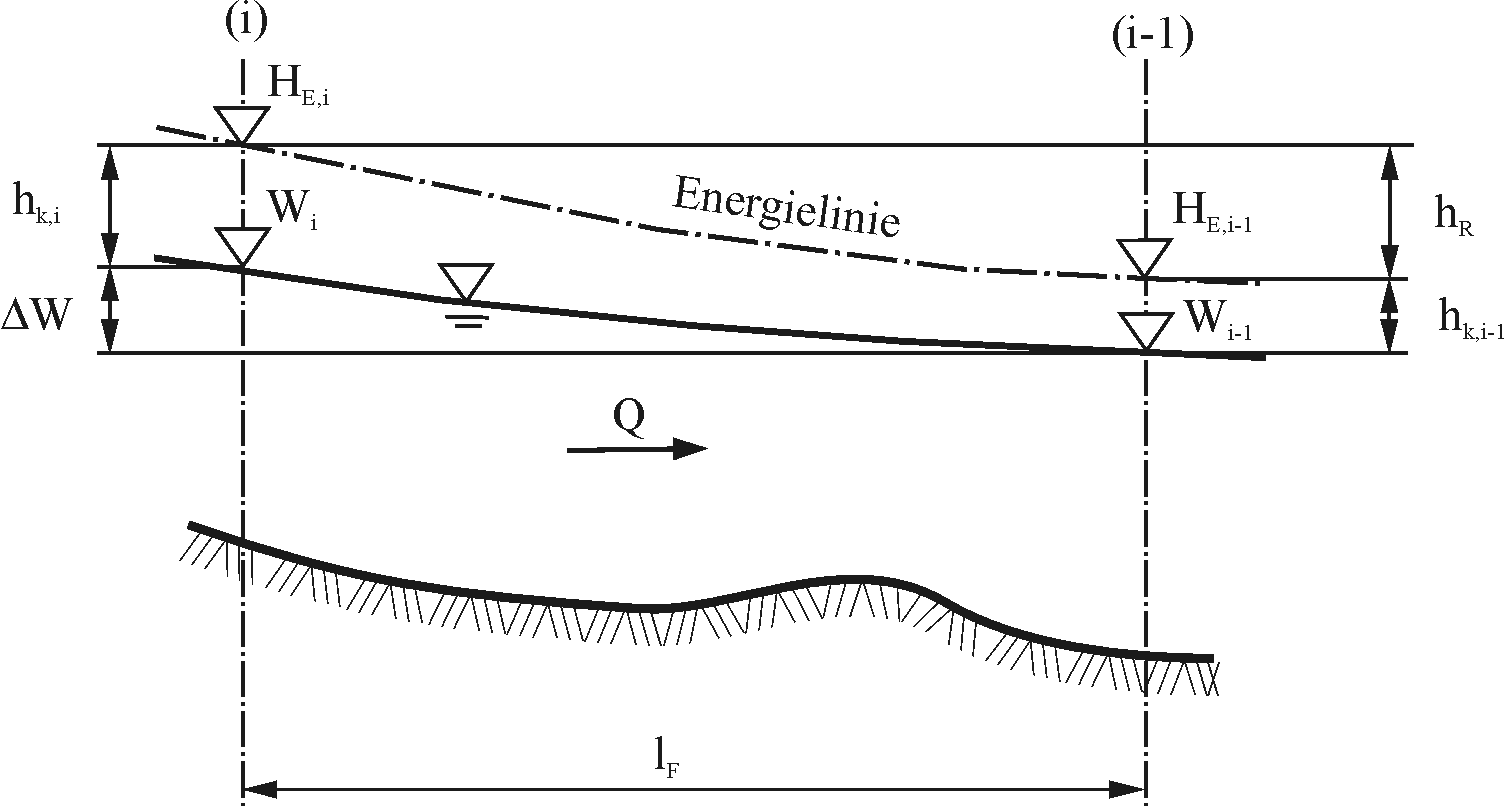
\includegraphics[scale=0.20]{Flussabschnitt}
   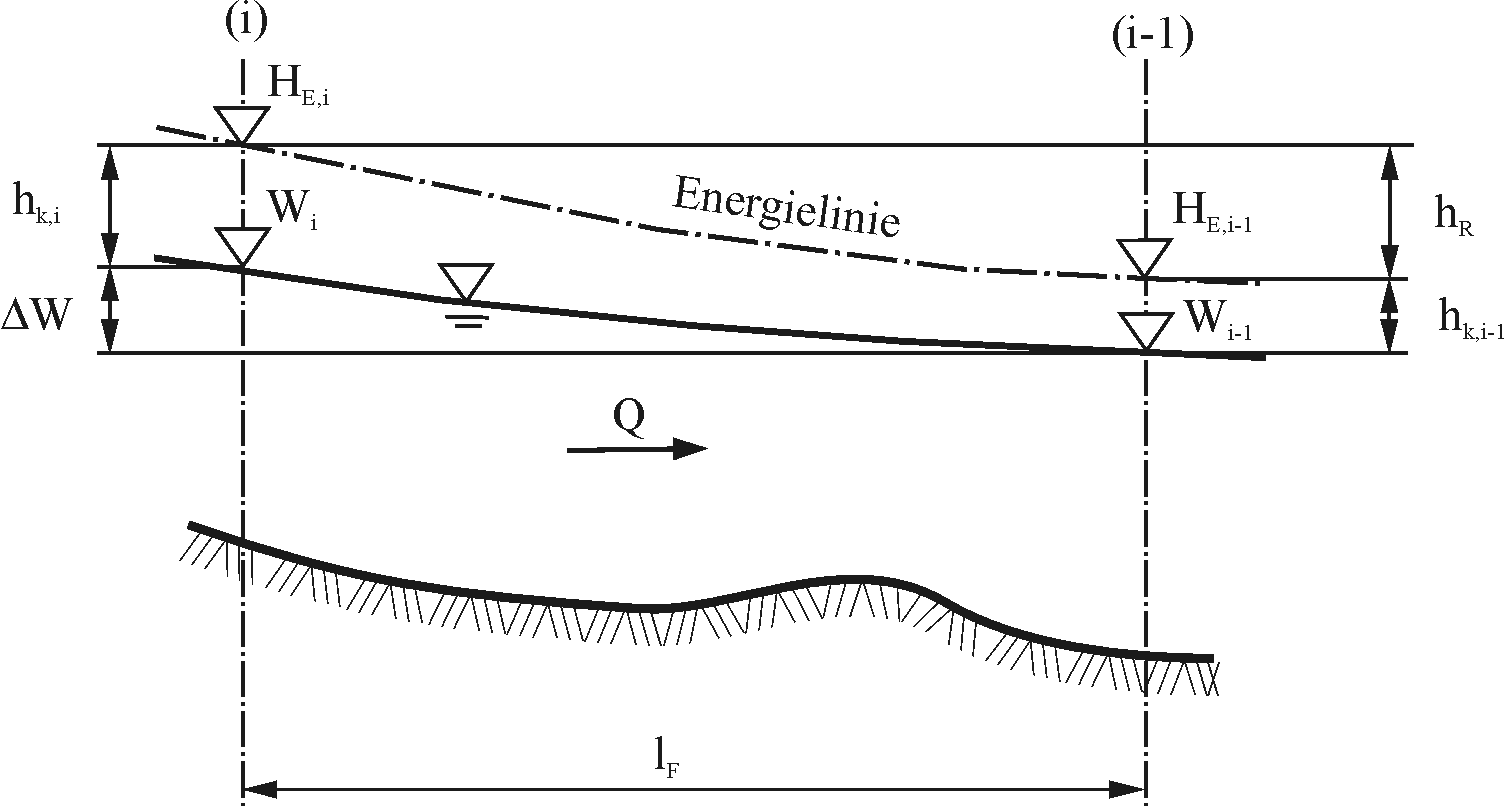
\includegraphics[width=0.8\linewidth]{Flussabschnitt}
   \caption{Flu{\ss}abschnitt $l_F$ mit Wasserspiegel und Energielinie}
   \label{Einfuehrung Abb Flussabschnitt}
\end{figure}
Mit den Bezeichnungen aus Abbildung~\ref{Einfuehrung Abb Flussabschnitt} ist
\begin{equation}
    W_i + h_{k,i}  =  W_{i-1} + h_{k,i-1} + h_R + H_{ZV}
\end{equation}
woraus sich durch einfache Umformung die Arbeitsgleichung ergibt:
\begin{equation}
    \Delta W  =  \Delta h_k + I_{E,m} \cdot l_F + H_{ZV}
\end{equation}
Hierbei bedeuten:
\begin{eqnarray*}
   \begin{tabular}{ll}
      $\Delta W = W_i - W_{i-1}$                               &  Differenz der Wasserst\"{a}nde \\
      $\Delta h_k = h_{k,i} - h_{k,i-1}$                       &  Differenz der Geschwindigkeitsh\"{o}hen \\
      $I_{E,m} = 0,5 \cdot (I_{E,i} + I_{E,i-1}) = h_R/l_F$    &  Mittleres Reibungsgef\"{a}lle \\
      $l_F$ 																									 & Profilabstand \\
      $H_{ZV}$                                                 &  Zus\"{a}tzliche \"{o}rtliche Verlusth\"{o}he
   \end{tabular}
\end{eqnarray*}
Die numerische L\"{o}sung dieser Gleichung erfolgt iterativ. Zun\"{a}chst wird aus dem Profilabstand und dem
Energieliniengef\"{a}lle des Profils~(i-1) der Wasserstandzuwachs $dh$ f\"{u}r das Profil~(i) gesch\"{a}tzt. F\"{u}r die sich dadurch
ergebende Wasserspiegelh\"{o}he $W_i = W_{i-1} + dh$ werden die erforderlichen geometrischen und hydraulischen Werte des
Profils~(i) berechnet. Mit dem daraus resultierenden Energieliniengef\"{a}lle $I_{E,i}$ kann die Verlusth\"{o}he ermittelt
werden, die zusammen mit der errechneten \"{A}nderung der Geschwindigkeitsh\"{o}he $dh_k$ eine neue Wasserspiegel\"{a}nderung $dW$
ergibt. Der Zuwachs $dh$ wird solange verbessert, bis sich dieser von dem errechneten Zuwachs $dW$ h\"{o}chstens um den
Wert der vereinbarten Genauigkeitsschranke $\mathit{EPSH}$ unterscheidet. In der Regel wird $\mathit{EPSH}$ zu
$0,005\unit{m}$ gew\"{a}hlt.

\subsection{Vorarbeiten}
Die zur Nachbildung der nat\"{u}rlichen Verh\"{a}ltnisse erforderlichen Vermessungsaufnahmen sollten bereits auf die
rechentechnischen M\"{o}glichkeiten des eingesetzten Wasserspiegellagenprogramms abgestimmt sein. Wenn eindimensionale
Rechenverfahren eingesetzt werden sollen, ist keine fl\"{a}chendeckende Gel\"{a}ndeaufnahme im Dezimeterbereich erforderlich, es
gen\"{u}gen Gel\"{a}nde-Querprofilaufnahmen in ausreichender Dichte.

Bei der Festlegung der Querprofile im Gel\"{a}nde ist den Besonderheiten, die sich aus der hydraulischen Problemstellung
ergeben, Rechnung zu tragen. Dies sind in erster Linie \"{U}berlegungen bez\"{u}glich des Querprofilabstandes, der Lage der
Profile im Lageplan, sowie der Ber\"{u}cksichtigung von Einbauten und sonstigen nat\"{u}rlichen Gegebenheiten wie z.B. Ufergeb\"{u}sch
oder Baumbewuchs. Wenn der Bewuchszustand einen merkbaren Einflu{\ss} auf das Str\"{o}mungsverhalten erwarten l\"{a}{\ss}t, so sind die
Buschgruppen und Baumreihen im Lageplan f\"{u}r eine Auswertung mit den entsprechenden Berechnungsverfahren mit aufzunehmen
(Abbildung~\ref{Einfuehrung Abb LageplanBewuchs}).

Bei Gerinneformen, die entsprechend einem Regelprofil ausgebaut worden sind, k�nnen gr��ere Profilabst�nde (l = 20 - 30 b) gew�hlt werden, bei sehr unregelm��iger Geometrie mit der M�glichkeit von schie�endem Abflu� k�nnen Profilabst�nde im Bereich der Gerinnebreite notwendig werden.
Grunds�tzlich sollte die Vermessung Querprofile in Flie�richtung gesehen liefern, d.h. in der Darstellung der Querprofile sollte das linke Vorland auch auf der linken Seite dar\-ge\-stellt sein.

\begin{figure}[hbt]
   \centering
   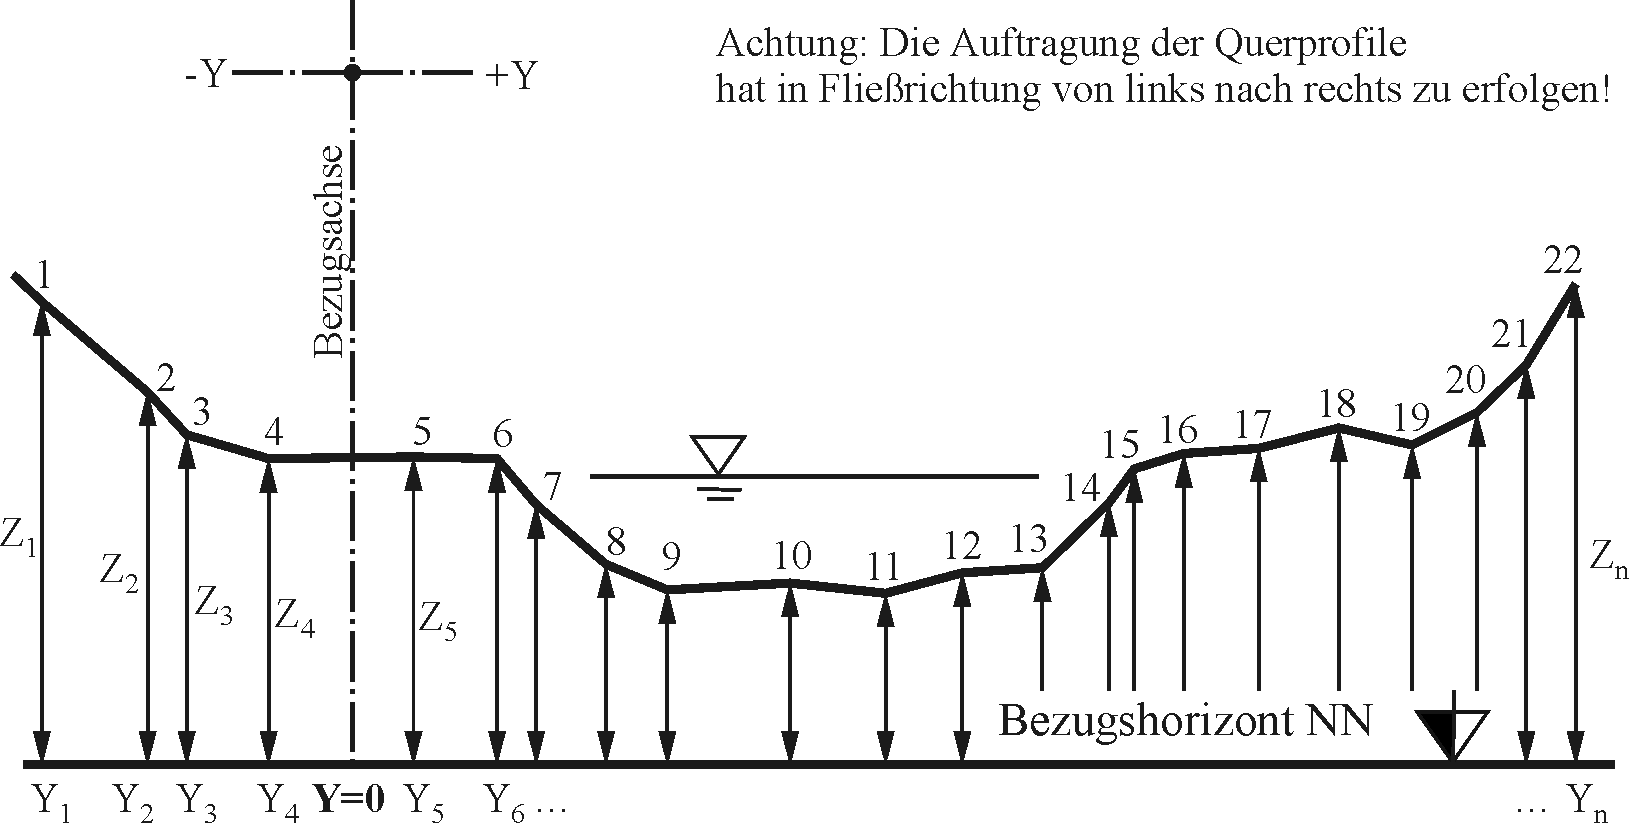
\includegraphics[width=0.8\linewidth]{ProfilaufnahmeKoordinaten}
   \caption{Beispiel einer Querprofilaufnahme (Eingabe in Koordinaten)}
   \label{Einfuehrung Abb Querprofilaufnahme}
\end{figure}
\begin{figure}[hbt]
   \centering
   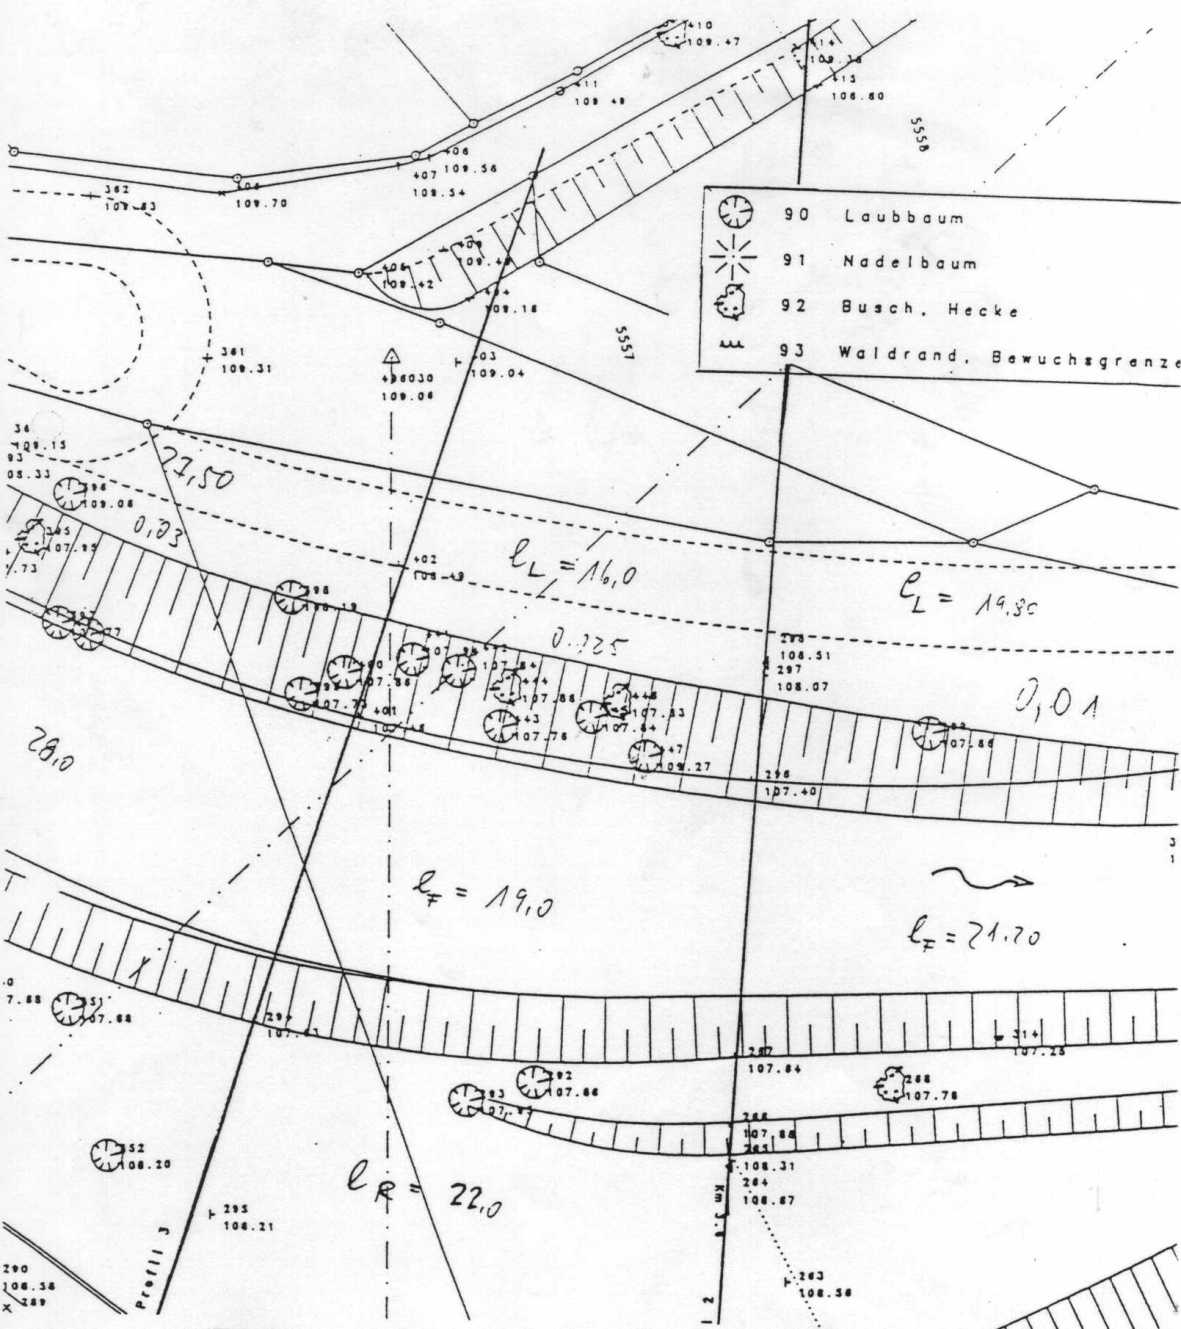
\includegraphics[width=0.8\linewidth]{LageplanBewuchs}
   \caption{Ausschnitt aus einem Lageplan mit eingezeichnetem Bewuchs}
   \label{Einfuehrung Abb LageplanBewuchs}
\end{figure}
Als Querprofildaten werden die Koordinaten des Profilpolygons ben\"{o}tigt:
\begin{itemize}
   \item horizontale Abst\"{a}nde der Profilpunkte ($y$-Werte) in $[\mathrm{m}]$ von einer beliebigen Bezugsachse
         (mit Vorzeichen einzugeben)
   \item H\"{o}he der Profilpunkte ($z$-Werte) in [$\mathrm{NN\!+\!m}$]
\end{itemize}
Liegen die Anfangs- bzw. Endpunkte des Profilpolygons unter dem berechneten Wasserspiegel, wird eine fiktive lotrechte
Begrenzung angenommen. Diese fiktive Begrenzung geht nicht in den benetzten Umfang ein, d.h. sie wird als reibungsfrei
betrachtet. Die Lage der Bezugsachse f\"{u}r die $y$-Werte ist beliebig. Es ist lediglich zu beachten, da{\ss} die Werte auf der
linken Seite der Achse ein negatives Vorzeichen haben m\"{u}ssen. Eine Variante f\"{u}r die Eingabe besteht darin, einen
Teilabflu{\ss}querschnitt des Flu{\ss}schlauchs in integraler Form einzugeben.

W\"{a}hrend f\"{u}r den Flu{\ss}schlauch der Abstand i.a. durch die Stationierung festgelegt ist, k\"{o}nnen bei den Vorlandteilfl\"{a}chen in
Flu{\ss}kr\"{u}mmungen hiervon abweichende Abst\"{a}nde auftreten. Aus diesem Grund ist es m\"{o}glich, die Abst\"{a}nde der Teilabflu{\ss}fl\"{a}chen
(linkes Vorland, Flu{\ss}schlauch, rechtes Vorland) getrennt einzugeben. Der Abstand wird dabei vom betrachteten
Profil~$(i-1)$ zum n\"{a}chsten oberstromigen Profil~$(i)$ gemessen. Als Abstand im Vorland kann die abgewickelte L\"{a}nge der
mittleren Strombahn des Vorlandteilabflusses betrachtet werden. Von besonderer Bedeutung ist hierbei, da{\ss} die
Abflu{\ss}verteilung in einem gegliederten Querschnitt von dem Verh\"{a}ltnis der Abst\"{a}nde zueinander abh\"{a}ngt. Ma{\ss}gebend f\"{u}r die
Abflu{\ss}verteilung im Querschnitt~$(i)$ sind die im Strang Profil~$(i-1)$ bis Profil~$(i)$ in der Strangtabelle angegebenen
Abst\"{a}nde.
         %  Kapitel  2
   \graphicspath{{./Installation/eps/}} 

\cleardoublepage
%%%%%%%%%%%%%%%%%%%%%%%%%%%%%%%%%%%%%%%%%%%%%%%%%%%%%%%%%%%%%%%%%%%%%%%%%%%%%%%%%%%%%%%%%%%%%%%%%%%%%%%%%%%%%%%%%%%%%%%%%%%%

\chapter{Installationshinweise}

\wspwin\ wird f�r die Betriebssysteme Windows NT, 2000 und XP vertrieben.

%%%%%%%%%%%%%%%%%%%%%%%%%%%%%%%%%%%%%%%%%%%%%%%%%%%%%%%%%%%%%%%%%%%%%%%%%%%%%%%%%%%%%%%%%%%%%%%%%%%%%%%%%%%%%%%%%%%%%%%%%%%%

%%%%%%%%%%%%%%%%%%%%%%%%%%%%%%%%%%%%%%%%%%%%%%%%%%%%%%%%%%%%%%%%%%%%%%%%%%%%%%%%%%%%%%%%%%%%%%%%%%%%%%%%%%%%%%%%%%%%%%%%%%%%
\section{Installation}
%%%%%%%%%%%%%%%%%%%%%%%%%%%%%%%%%%%%%%%%%%%%%%%%%%%%%%%%%%%%%%%%%%%%%%%%%%%%%%%%%%%%%%%%%%%%%%%%%%%%%%%%%%%%%%%%%%%%%%%%%%%%

Ab der Version \wspwin{~4.0} werden die Windows-Oberfl\"{a}chen, das Berechnungsprogramm sowie evtl. Zusatzprogramme in einem
Installationsvorgang von CD-ROM auf Ihrem Rechner installiert. Davon ausgenommen sind allerdings \wspwin{}-Plotter und
\wspwin{}-Mapper, die separat installiert werden m\"{u}ssen. Starten Sie \"{u}ber den Windows-Explorer die Datei
\datei{setup.exe}. Der Installationsmanager geleitet Sie nun durch die Programminstallation.
\begin{figure}
   \centering
   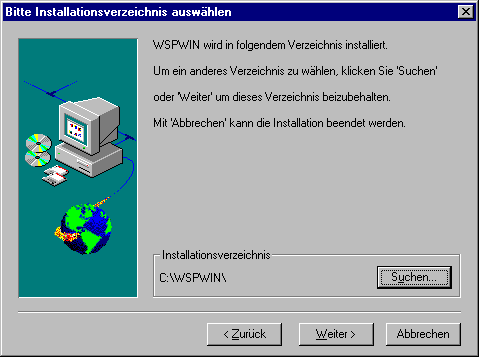
\includegraphics[width=0.9\linewidth]{Installationspfad}
   \caption{Auswahl des Installationspfades}
   \label{Installation Abb Installationspfad}
\end{figure}
Die Installation bietet standardm\"{a}{\ss}ig das Verzeichnis \datei{C:\textbackslash WSPWIN} als Installationsverzeichnis an.
Soll die Installation in einem anderen Verzeichnis erfolgen, dr\"{u}cken sie \schalter{Suchen...} und w\"{a}hlen das neue
Installationsverzeichnis oder geben den Pfad von Hand ein.

Grunds\"{a}tzlich bestehen \"{u}ber das Installationsprogramm die im folgenden beschriebenen vier M\"{o}glichkeiten der Installation:
\begin{figure}
   \centering
   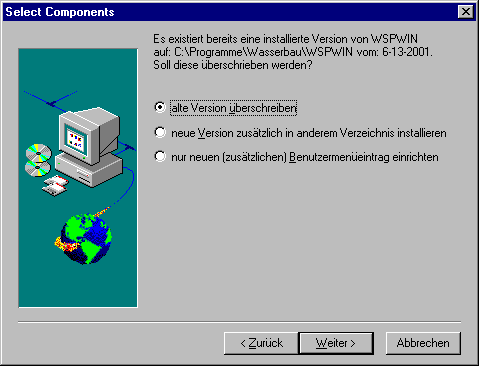
\includegraphics[width=0.9\linewidth]{Optionen}
   \caption{Installationsoptionen}
   \label{Installation Abb Optionen}
\end{figure}

\subsubsection{Erstinstallation} Es wurde keine \wspwin{}-Programmdatei vom Setup-Programm vorgefunden. Sie haben die
M\"{o}glichkeit zu entscheiden, ob nur \wspwin{} oder auch HYDRA-Programme (bei Erwerb) bzw. Demoprojekte installiert werden
sollen.

\subsubsection{Anlegen eines Updates}
Das Setup-Programm \"{u}berschreibt die alten Dateien im selben Verzeichnis. Besser ist es jedoch, das alte Programm zu
deinstallieren (vgl. Abschnitt~\ref{Installation Sec Deinstallation}) und im Anschlu{\ss} daran eine Neuinstallation
durchzuf\"{u}hren.

\subsubsection{Zweitinstallation in einem anderen Verzeichnis}
Beachten Sie bei der Wahl eines Programmgruppensymbols, da{\ss} Sie nach M\"{o}glichkeit kein bereits existierendes Symbol
verwenden. Die Verkn\"{u}pfung bezieht sich sonst nur auf das zuletzt installierte Programm.

\clearpage
Die DOS-Programme f\"{u}r hydraulische Bemessungen werden ab Version~4.0 in dem Unterverzeichnis HYDRA mit
installiert. In der Datei autoexec.bat erfolgt automatisch ein Eintrag mit einer SET-Anweisung, z.B.:
\begin{quote}
   \datei{REM HYDRA-Softwareeintrag 7-24-2001 BEGIN \\
          SET HYDRA = C:\textbackslash WSPWIN \textbackslash HYDRA \\
          REM HYDRA-Softwareeintrag END}
\end{quote}
Nach Beendigung der Installation fordert Sie das Setup-Programm zum Neustart ihres Computers auf. Bei der Erstinstallation
werden standardm\"{a}{\ss}ig alle Programme, die nicht im unmittelbaren Zusammenhang mit dem Wasserspiegellagenprogramm stehen
(z.B. Sonderprogramme \datei{gerinne}, \datei{rohre}, \datei{wehre}), in das Unterverzeichnis \datei{...\textbackslash
Hydra} kopiert. F\"{u}r Programmdateien, Hilfedateien und Daten existieren eigene Unterverzeichnisse. Eigene Daten k\"{o}nnen in
beliebige, vom Nutzer erstellte Verzeichnisse geschrieben werden.

F\"{u}r den Programmzugriff von anderen Unterverzeichnissen (d.h. auch aus \wspwin{}  he\-raus) kann der Path-Befehl in der
\datei{autoexec.bat} durch
\begin{quote}
   \datei{C:\textbackslash WSPWIN\textbackslash HYDRA} \hspace{0.5cm} und \\
   \datei{C:\textbackslash WSPWIN}
\end{quote}
erg\"{a}nzt werden.

Die Verzeichnisstruktur f\"{u}r HYDRA zeigt Tabelle~\ref{Installation Tab VerzeichnisHydra}. Neben dem Standardpaket k\"{o}n\-nen
Zusatzprogramme f\"{u}r Entlastungsbauwerke und Stra{\ss}enbau erworben werden. Diese erhalten dann ebenfalls jeweils ein eigenes
Unterverzeichnis (\datei{...\textbackslash Atv} und \datei{...\textbackslash Stra}) f\"{u}r die Daten.
\begin{table}
   \centering
   \input{Installation/tab/HydraVerzeichnis.tab}
   \caption{Verzeichnisstruktur f\"{u}r HYDRA}
   \label{Installation Tab VerzeichnisHydra}
\end{table}
In den Dateien \datei{Hydra.kdd} und \datei{Kopf.txt} ist die Firmenanschrift festgelegt. Die ersten drei Zeilen d\"{u}rfen
nicht ge\"{a}ndert werden, da die Programmdateien zur jeweiligen \datei{Kopf.txt} passen m\"{u}ssen. F\"{u}r Arbeiten unter DOS kann
in Zeile~5 der gew\"{u}nschte Editor definiert werden, der vom Men\"{u} aus aufgerufen werden soll. Die Zeilen~6 und 7 enthalten
die Bezeichnung der Standardunterverzeichnisse f\"{u}r die Speicherung von Daten der ATV-Programme bzw.
Stra{\ss}enbau-Dialogprogramme.

Einen \"{U}berblick \"{u}ber die Dateien im Installationsverzeichnis (z.B. \datei{C:\textbackslash WSPWIN}) und ihre Funktion gibt
die Tabelle~\ref{Installation Tab Dateien}.
\begin{table}
   \centering
   \input{Installation/tab/Installationsverzeichnis.tab}
   \caption{Dateien im Installationsverzeichnis}
   \label{Installation Tab Dateien}
\end{table}

\begin{table}
   \centering
   \input{Installation/tab/Systemdateien.tab}
   \caption{Dateien im Systemverzeichnis von Windows}
   \label{Installation Tab DateienSystem}
\end{table}

%%%%%%%%%%%%%%%%%%%%%%%%%%%%%%%%%%%%%%%%%%%%%%%%%%%%%%%%%%%%%%%%%%%%%%%%%%%%%%%%%%%%%%%%%%%%%%%%%%%%%%%%%%%%%%%%%%%%%%%%%%%%
\section{Installation im Netz}
%%%%%%%%%%%%%%%%%%%%%%%%%%%%%%%%%%%%%%%%%%%%%%%%%%%%%%%%%%%%%%%%%%%%%%%%%%%%%%%%%%%%%%%%%%%%%%%%%%%%%%%%%%%%%%%%%%%%%%%%%%%%

Bei Erwerb einer Mehrfachlizenz kann \wspwin{} auch im Netz installiert und von verschiedenen Rechnern aus genutzt werden.
Hierf\"{u}r ist allerdings im Windows-Verzeichnis eines jeden PC's, von dem aus auf \wspwin{} zugegriffen werden soll, ein
zus\"{a}tzlicher Eintrag vorzunehmen. Automatisch wird dieser nur auf dem Rechner eingetragen, von dem aus die Installation
durchgef\"{u}hrt wird. Der Eintrag zeigt an, wo sich die Projektverwaltungsdatei \datei{Wsp.prj} befindet, in der s\"{a}mtliche
von \wspwin{} aus angelegten Projekte aufgelistet werden. Der Eintrag lautet:
\begin{quote}
   \datei{[WSPWIN]} \\
   \datei{PRJPATH=C:\textbackslash WSPWIN} (bzw. individueller Pfad, wo \datei{Wsp.prj} steht)
\end{quote}
Der Eintrag befindet sich in einer eigenen Datei \datei{wspwin.ini} im Windows-Verzeichnis. In Abh\"{a}ngigkeit davon, ob
verschiedene Benutzer auf die gleichen Projekte Zugriff haben sollen, oder von jedem Rechner aus unterschiedliche Projekte
bearbeitet werden, kann die \datei{Wsp.prj}-Datei (standardm\"{a}{\ss}ig im \wspwin{}-Verzeichnis) in ein beliebiges Verzeichnis
im Netz oder lokal gelegt werden. Der Eintrag ist dann anzupassen. Es ist allerdings davon abzuraten, da{\ss} mehrere Benutzer
gleichzeitig auf die selben Projekte zugreifen.


%%%%%%%%%%%%%%%%%%%%%%%%%%%%%%%%%%%%%%%%%%%%%%%%%%%%%%%%%%%%%%%%%%%%%%%%%%%%%%%%%%%%%%%%%%%%%%%%%%%%%%%%%%%%%%%%%%%%%%%%%%%%
\section{Benutzerdefinierte Einstellungen}
%%%%%%%%%%%%%%%%%%%%%%%%%%%%%%%%%%%%%%%%%%%%%%%%%%%%%%%%%%%%%%%%%%%%%%%%%%%%%%%%%%%%%%%%%%%%%%%%%%%%%%%%%%%%%%%%%%%%%%%%%%%%

Nach dem ersten Programmstart k\"{o}nnen unter dem Men\"{u}punkt \menu{\marrow E\underline{x}tras \marrow \underline{O}ptionen}
weitere Einstellungen vorgenommen werden.

\begin{figure}
   \centering
   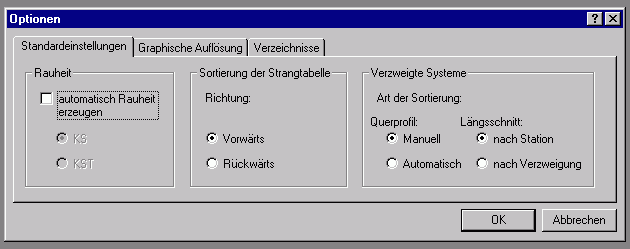
\includegraphics[width=0.9\linewidth]{extras_optionen}
   \caption{Benutzerdefinierte Einstellm�glichkeiten}
   \label{Installation Abb extras_optionen}
\end{figure}

\subsection{Standardeinstellungen}
\label{Installation Subsec Standardeinstellungen}

Beim Erstellen von Querprofilen besteht die M�glichkeit standardm��ig die Datens�tze Gel�ndeh�he, Trennfl�chen, Durchstr�mte Bereiche und Rauheiten automatisch anzulegen. Die Registerkarte Standardeinstellungen bietet Ihnen die M�glichkeit, festzulegen, welche Rauheiten, nach \autor{Darcy-Weisbach} oder \autor{Manning-Strickler}, hierf�r zugrundegelegt werden sollen (siehe auch Abschnitt~\ref{Einstieg Subsec Rauheit}). 

Ferner haben Sie hier die M�glichkeit die Art der Sortierreihenfolge f�r das Neuanlegen und Aufnehmen von Profilen festzulegen. Standardm��ig erfolgt die Sortierung der Strangtabelle von der niedrigsten zu h�chsten Station (Vorw�rts). Da einzelne Gew�sser aber auch von der M�ndung zu Quelle hin stationiert sind, haben Sie an dieser Stelle die M�glichkeit, die automatische Sortierreihenfolge umzukehren.

Weiterhin k�nnen Sie Festlegungen zur Sortierreihenfolge der Querprofile in verzweigten Systemen treffen (siehe hierzu auch Ab\-schnitt~\ref{Sonderprofile Sec VerzweigteSysteme}).


\subsection{Grafische Aufl\"{o}sung}
Hier k\"{o}nnen sie die Aufl\"{o}sung Ihres Bildschirms manuell einstellen. Die Voreinstellung steht auf automatischer Erkennung.
Die Darstellung der Masken ist optimal bei einer Grafikaufl\"{o}sung von $1024\times768~\mathrm{Pixel}$, wobei eine kleine
Schrift mit einer Skalierung von $100\%$ einzustellen ist.

\subsection{Verzeichnisse}
\label{Installation Subsec Verzeichnisse}
\begin{description}
   \item[Hauptverzeichnis:]
      Das Hauptverzeichnis wird immer dann ge\"{o}ffnet, wenn Sie ein neues Projekt anlegen. Geben Sie hier den Pfad zu dem
      Ordner ein, in dem sie normalerweise Ihre Projekte ablegen.
\end{description}
\begin{hinweis}
   Um Probleme beim Erstellen eines Projektes zu vermeiden, verwenden Sie keine langen Verzeichnisnamen mit Umlauten oder
   Sonderzeichen. M\"{o}chten Sie Ihre Projekte z.B. unter \datei{C:\textbackslash Eigene Dateien} ablegen, so verwenden Sie
   den DOS-Namen, beispielsweise \datei{C:\textbackslash Eigene$\sim$1}, des Verzeichnisses.
\end{hinweis}

\wspwin{} bietet die M\"{o}glichkeit, direkt aus der Oberfl\"{a}che heraus externe Programme zu starten. Damit \wspwin{} wei{\ss}, wo
sich Ihr Programm befindet, haben Sie hier die M\"{o}glichkeit, den entsprechenden Pfad anzugeben.
\begin{description}
   \item[Editor:]
      Geben sie hier den Pfad zu einem externen Texteditor ein. Dieser wird \"{u}ber das Men\"{u}
      \menu{\marrow \underline{E}rgebnisse \marrow \underline{E}ditor}
      aufgerufen.
   \item[CAD-Programm:]
      Geben sie hier den Pfad zu einem CAD-Programm an, das sie normalerweise verwenden. \"{U}ber das Men\"{u}
      \menu{\marrow P\underline{l}otten \marrow \underline{C}AD-Programm} k\"{o}nnen Sie das Programm starten und so von
      \wspwin{} erstellte dxf-Dateien bearbeiten.
   \item[Sonderprogramm:]
      Hier haben sie die M\"{o}glichkeit den Pfad f\"{u}r ein beliebiges externes Programm anzugeben, das aus \wspwin{} heraus
      gestartet werden soll. Der Programmaufruf erfolgt \"{u}ber den Men\"{u}punkt \menu{\marrow E\underline{x}tras \marrow
      \underline{S}onderprogramm}.
\end{description}


%%%%%%%%%%%%%%%%%%%%%%%%%%%%%%%%%%%%%%%%%%%%%%%%%%%%%%%%%%%%%%%%%%%%%%%%%%%%%%%%%%%%%%%%%%%%%%%%%%%%%%%%%%%%%%%%%%%%%%%%%%%%
\section{Deinstallation}
\label{Installation Sec Deinstallation}
%%%%%%%%%%%%%%%%%%%%%%%%%%%%%%%%%%%%%%%%%%%%%%%%%%%%%%%%%%%%%%%%%%%%%%%%%%%%%%%%%%%%%%%%%%%%%%%%%%%%%%%%%%%%%%%%%%%%%%%%%%%%

Windows~95/NT bietet die M\"{o}glichkeit der Deinstallation. Nach der Installation erscheinen im Startmen\"{u} unter dem
Programmgruppensymbol Spiegellinienberechnung (vgl. Abbildung~\ref{Einstieg Abb Programmstart}) zwei Eintr\"{a}ge:
\begin{quote}
   \menu{WSPWIN}, \"{u}ber das Sie das Programm starten k\"{o}nnen, und \\[6pt]
   \menu{UnInstallShield}, das es erm\"{o}glicht, die Software wieder zu l\"{o}schen.
\end{quote}
Die Eintr\"{a}ge in der Datei \datei{autoexec.bat} bleiben jedoch auch nach dem Ausf\"{u}hren des Deinstallationsprogramms
bestehen. Um sie zu entfernen, \"{o}ffnen sie die Dateien in einem Editor und entfernen die Eintr\"{a}ge von Hand. Danach m\"{u}ssen
sie den Computer neu starten.
        %  Kapitel  3
   \graphicspath{{Einstieg/eps/}} \cleardoublepage
%%%%%%%%%%%%%%%%%%%%%%%%%%%%%%%%%%%%%%%%%%%%%%%%%%%%%%%%%%%%%%%%%%%%%%%%%%%%%%%%%%%%%%%%%%%%%%%%%%%%%%%%%%%%%%%%%%%%%%%%%%%%

\chapter{Der Einstieg in die Handhabung}
\label{Einstieg}

%%%%%%%%%%%%%%%%%%%%%%%%%%%%%%%%%%%%%%%%%%%%%%%%%%%%%%%%%%%%%%%%%%%%%%%%%%%%%%%%%%%%%%%%%%%%%%%%%%%%%%%%%%%%%%%%%%%%%%%%%%%%

Im folgenden werden die einzelnen Funktionen von \wspwin{} n\"{a}her erl\"{a}utert. Die Ausf\"{u}h\-rungen orientieren sich an der
Men\"{u}struktur des Programms. Diese ist entsprechend der im Rahmen einer Spiegellinienberechnung nacheinander auszuf\"{u}hrenden
Arbeitsschritte aufgebaut. Das bedeutet, da{\ss} das Programm von links nach rechts in der Men\"{u}leiste durchzuarbeiten ist.

So wird zuerst ein Projekt angelegt, danach eine Zustandsdatei und schlie{\ss}lich werden Profile erstellt und bearbeitet.
Anschlie{\ss}end ist eine Abflu{\ss}datei zu erzeugen (Randbedingungen), bevor im letzten Schritt die eigentliche Berechnung
ausgef\"{u}hrt werden kann. Um das Arbeiten mit \wspwin{} zu erlernen, sollten Sie die nachfolgend erl\"{a}uterten
Programmoptionen, wie beschrieben, durcharbeiten. Dabei ist es sinnvoll, zun\"{a}chst alle als Zusatzoptionen in den
nachfolgenden Kapiteln aufgef\"{u}hrten Funktionen auszulassen und diese erst n\"{a}her zu betrachten, nachdem einmal eine
komplette Berechnung durchgespielt wurde.


%%%%%%%%%%%%%%%%%%%%%%%%%%%%%%%%%%%%%%%%%%%%%%%%%%%%%%%%%%%%%%%%%%%%%%%%%%%%%%%%%%%%%%%%%%%%%%%%%%%%%%%%%%%%%%%%%%%%%%%%%%%%
\section{Das Starten des Programms}
%%%%%%%%%%%%%%%%%%%%%%%%%%%%%%%%%%%%%%%%%%%%%%%%%%%%%%%%%%%%%%%%%%%%%%%%%%%%%%%%%%%%%%%%%%%%%%%%%%%%%%%%%%%%%%%%%%%%%%%%%%%%

Nach der Installation kann das Programm durch Aktivierung des Programmsymbols \menu{Spiegellinienberechnung} im Startmen\"{u}
der Task-Leiste aktiviert werden. Hier finden sich zwei Untermen\"{u}punkte \menu{\marrow WSPWIN} zum Starten und
\menu{\marrow UnInstallShield} zum L\"{o}schen des Programms.
\begin{figure}[hbt]
    \centering
    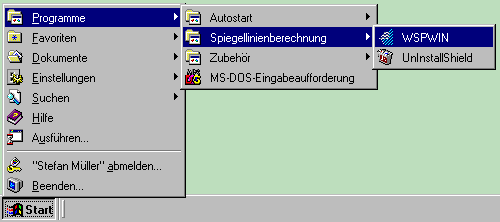
\includegraphics[width=0.8\textwidth]{Windows_Start}
    \caption{Programmstart unter Windows}
    \label{Einstieg Abb Programmstart}
\end{figure}


\clearpage
%%%%%%%%%%%%%%%%%%%%%%%%%%%%%%%%%%%%%%%%%%%%%%%%%%%%%%%%%%%%%%%%%%%%%%%%%%%%%%%%%%%%%%%%%%%%%%%%%%%%%%%%%%%%%%%%%%%%%%%%%%%%
\section{Projekte bearbeiten}
%%%%%%%%%%%%%%%%%%%%%%%%%%%%%%%%%%%%%%%%%%%%%%%%%%%%%%%%%%%%%%%%%%%%%%%%%%%%%%%%%%%%%%%%%%%%%%%%%%%%%%%%%%%%%%%%%%%%%%%%%%%%

\begin{figure}[ht]
   \centering
   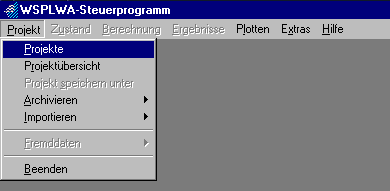
\includegraphics{MenueProjekte}
   \caption{Der Men\"{u}punkt Projekt}
   \label{Einstieg Abb MenueProjekt}
\end{figure}


\subsection{Ein neues Projekt anlegen}

Nach dem Start des Programms gelangen Sie \"{u}ber das Men\"{u} \menu{\marrow \underline{P}rojekt \marrow \underline{P}rojekte} in
die \dialog{Projektauswahlmaske} (Abbildung~\ref{Einstieg Abb Projektauswahlmaske}). Sie m\"{u}ssen nun zun\"{a}chst ein
bestehendes Projekt \"{o}ffnen oder ein neues Projekt, d.h. Verzeichnis, erstellen. In diesem Verzeichnis werden alle
nachfolgenden Arbeiten gespeichert. Bei sp\"{a}teren Arbeiten k\"{o}nnen Sie dann entscheiden, ob diese im selben Verzeichnis
abgelegt werden sollen (dann ist nur das bereits existierende Projekt zu \"{o}ffnen), oder ob sie f\"{u}r die neuen Arbeiten
wieder ein neues Verzeichnis einrichten m\"{o}chten.
\begin{figure}[hbt]
    \centering
    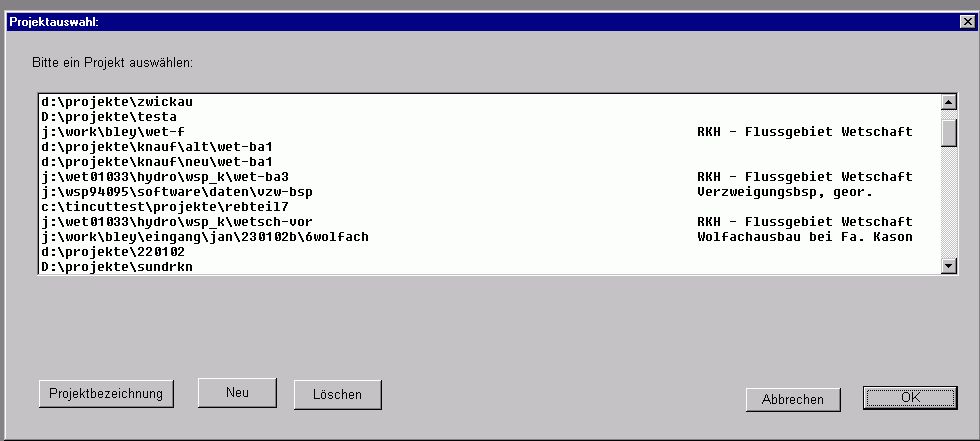
\includegraphics[width=1.0\textwidth]{Projektauswahl}
    \caption{Die Projektauswahlmaske}
    \label{Einstieg Abb Projektauswahlmaske}
\end{figure}

\"{U}ber die Schaltfl\"{a}che \schalter{Neu} gelangen sie in den Dialog zur Erstellung eines neuen Projektes
(Abbildung~\ref{Einstieg Abb ProjektErstellen}). Zu Ihrer Information ist im oberen Teil der Maske der Pfadname des
Verzeichnisses aufgef\"{u}hrt, in dem Sie zuletzt gearbeitet haben. Sie k\"{o}nnen unter dem Men\"{u}punkt \menu{\marrow
E\underline{x}tras \marrow \underline{O}ptionen} ein Hauptverzeichnis angeben, das Ihnen immer als
Standarddatenverzeichnis an dieser Stelle erscheint, um z.B. alle Projekte in einem extra \wspwin{}-Projektordner
abzulegen (siehe auch Abschnitt~\ref{Installation Subsec Verzeichnisse}).
\begin{figure}
    \centering
    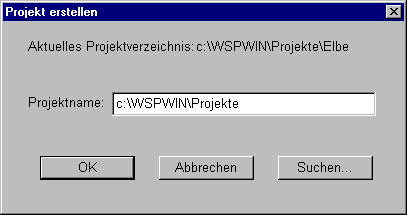
\includegraphics[width=0.6\textwidth]{ProjektErstellen}
    \caption{Anlegen eines neuen Projektes}
    \label{Einstieg Abb ProjektErstellen}
\end{figure}

Zum Anlegen eines neuen Projektordners geben sie den gew\"{u}nschten Pfad in das Eingabefeld ein und best\"{a}tigen die Eingabe
mit \schalter{OK}. Das neu erstellte Projekt erscheint nun in der \dialog{Projektauswahlmaske}. Ein Projekt stellt in
der Hierarchie der Dateiverwaltung die oberste Kategorie dar. S\"{a}mtliche weiteren Bearbeitungsschritte beziehen sich
anschlie{\ss}end auf das neu erstellte (bzw. ausgew\"{a}hlte) Projekt.
\begin{hinweis}
    In der Maske \dialog{Projekt erstellen}, die nach Bet\"{a}tigung der Schaltfl\"{a}che \schalter{Neu} aus der
    \dialog{Projektauswahlmaske} heraus erscheint, haben Sie auch die M\"{o}glichkeit \"{u}ber die Schaltfl\"{a}che \schalter{Suchen...}
    ein Verzeichnis \"{u}ber den Standard-Windows-Dialog im Verzeichnisbaum zu suchen.
    Im Anschlu{\ss} an die Selektion existierender Verzeichnisse k\"{o}nnen Sie im Editierfeld Verzeichnis ein oder mehrere
    Unterverzeichnisse angeben.
\end{hinweis}

\"{U}ber die Schaltfl\"{a}che \schalter{Projektbezeichnung} k\"{o}nnen sie jedem Projekt eine zus\"{a}tzliche Bezeichnung (maximal
60~Zeichen, Leerzeichen sind erlaubt) zuordnen. Diese Projektbezeichnung erscheint sp\"{a}ter auf dem Ausdruck Ihrer
Ergebnisdatei. Die Projektbezeichnung stellt f\"{u}r Sie auch eine M\"{o}glichkeit dar, Ihre Projekte unabh\"{a}ngig vom unter
Umst\"{a}nden nicht eindeutigen Pfadnamen leichter zu identifizieren.


\subsection{Projekt \"{o}ffnen}
\label{Einstieg Subsec ProjektOeffnen}

Wenn Sie den Men\"{u}punkt \menu{\marrow \underline{P}rojekt \marrow \underline{P}rojekte} gew\"{a}hlt haben, gelangen Sie
automatisch in die \dialog{Projektauswahlmaske}, aus der heraus ein Projekt auszuw\"{a}hlen bzw. zu \"{o}ffnen ist.

Wenn noch kein neues Projekt angelegt wurde, ist die Projektauswahlmaske leer, ansonsten werden alle verf\"{u}gbaren
Projekte aufgelistet. \"{U}ber den Schalter \schalter{OK} \"{o}ffnen Sie das markierte Projekt (vgl. Abbildung~\ref{Einstieg
Abb Projektauswahlmaske}). Ohne ein ge\"{o}ffnetes Projekt, k\"{o}nnen keine weiteren Arbeitsschritte ausgef\"{u}hrt werden. Alle
weiteren Arbeiten beziehen sich dann auf das ausgew\"{a}hlte Verzeichnis und werden in diesem abgespeichert. \"{U}ber die
Option \schalter{Projektbezeichnung} haben Sie die M\"{o}glichkeit, die Projektbezeichnung zu modifizieren (siehe auch
Abschnitt~\ref{Einstieg Subsec ProjektOeffnen}).


\subsection{Projekt l\"{o}schen}

Neben dem Anlegen eines neuen Projektes und dem \"{O}ffnen bereits existierender Projekte bietet die
\dialog{Projektauswahlmaske} auch die M\"{o}glichkeit, ein Projekt zu l\"{o}schen. Markieren Sie das zu l\"{o}schende Projekt in der
Auswahlliste und w\"{a}hlen Sie den Schalter \schalter{L\"{o}schen}. Es folgt eine Sicherheitsabfrage ob Sie wirklich das gesamte
Projekt l\"{o}schen m\"{o}chten. An dieser Stelle k\"{o}nnen Sie den L\"{o}schvorgang noch abbrechen.

Bitte beachten Sie, da{\ss} s\"{a}mtliche Dateien in den Unterverzeichnissen \datei{...\textbackslash prof} und
\datei{...\textbackslash dath} des entsprechenden Projekt-Verzeichnisses gel\"{o}scht werden. Existieren in dem
Projektverzeichnis zus\"{a}tzliche Dateien oder Verzeichnisse (z.B. vom Plotprogramm) bleiben diese vom L\"{o}schvorgang
unber\"{u}hrt. Beachten Sie weiterhin, da{\ss} das aktuelle Projektverzeichnis nicht gel\"{o}scht werden kann. Dies kann erst
erfolgen, wenn ein anderes Projekt ge\"{o}ffnet wurde. Sollte ein Verzeichnis nicht mehr existieren, kann nur der
Projekteintrag entfernt werden (vgl. \menu{\marrow \underline{P}rojekt \marrow \underline{I}mportieren \marrow
Projekteintrag \underline{l}\"{o}schen}).


\subsection{Beispiel}

Legen Sie das Projekt \afz{Beispiel} auf Ihrer Festplatte an. \"{O}ffnen Sie dazu zun\"{a}chst die Projektauswahlmaske
(Abbildung~\ref{Einstieg Abb Projektauswahlmaske}) \"{u}ber das Men\"{u} \menu{\marrow \underline{P}rojekt \marrow
\underline{P}rojekte}. Mit Hilfe der Schaltfl\"{a}che \schalter{Neu} gelangen sie in den Dialog zur Erstellung eines neuen
Projektes. Geben Sie hier Pfad und Verzeichnisnamen Ihres Projektes ein, z.B.
\begin{quote}
    \datei{C:\textbackslash WSPWIN \textbackslash Projekte\textbackslash Beispiel}
\end{quote}
und best\"{a}tigen die Eingabe mit \schalter{OK}. Das neu angelegte Projekt erscheint jetzt in der Projektauswahlmaske.
Markieren Sie es und \"{o}ffnen Sie das Verzeichnis mit Hilfe von \schalter{OK}.


\clearpage
%%%%%%%%%%%%%%%%%%%%%%%%%%%%%%%%%%%%%%%%%%%%%%%%%%%%%%%%%%%%%%%%%%%%%%%%%%%%%%%%%%%%%%%%%%%%%%%%%%%%%%%%%%%%%%%%%%%%%%%%%%%%
\section{Zustandsdatei bearbeiten}
%%%%%%%%%%%%%%%%%%%%%%%%%%%%%%%%%%%%%%%%%%%%%%%%%%%%%%%%%%%%%%%%%%%%%%%%%%%%%%%%%%%%%%%%%%%%%%%%%%%%%%%%%%%%%%%%%%%%%%%%%%%%

Sobald Sie ein Projekt ge\"{o}ffnet haben, erreichen Sie automatisch die n\"{a}chste Kategorie der Dateiverwaltung, die Zustands-
oder Vernetzungsdatei.
\begin{figure}[hptb]
    \centering
    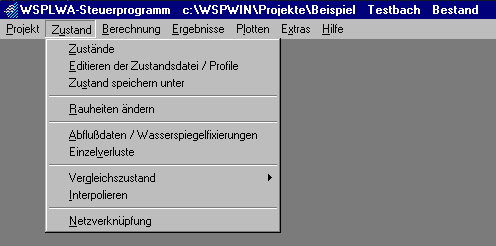
\includegraphics[width=0.7\textwidth]{MenueZustand}
    \caption{Das Men\"{u} Zustand}   \label{Einstieg Abb MenueZustand}
\end{figure}
Eine Zustandsdatei stellt die Verkn\"{u}pfung mehrerer Profildateien dar, die alle demselben geometrischen Zustand zugeh\"{o}rig
sind (z.B. Istzustand, Ausbauzustand, Bestand, Planung). Innerhalb eines Projektes k\"{o}nnen mehrere Zustandsdateien angelegt
werden, die ihrerseits wiederum unterschiedliche, aber auch gleiche Profile verwalten k\"{o}nnen.

\subsection{Eine neue Zustandsdatei anlegen}

Sofern Sie ein neues Projekt eingerichtet haben, sind in der Dialogmaske \dialog{Auswahl der Zustandsdatei} keine
Eintr\"{a}ge vorhanden. Um eine neue Zustandsdatei zu definieren, gelangen Sie \"{u}ber die Schaltfl\"{a}che
\schalter{Neue Zustandsdatei} in den Dialog \dialog{Neue Vernetzungsdatei anlegen}
(Abbildung~\ref{Einstieg Abb ZustandsdateiNeu}). Es erscheint eine Maske, die Sie zur Angabe des Gew\"{a}ssernamens, der Kennung
des Zustands, sowie des zuzuordnenden Datums auffordert.
\begin{hinweis}
   Vermeiden Sie beim Gew\"{a}ssernamen und Zustand Sonderzeichen, wie Punkt, Bindestrich, Unterstrich, Leerzeichen etc.,
   die bei sp\"{a}teren Bearbeitungsschritten zu Problemen f\"{u}hren k\"{o}nnen.
\end{hinweis}
Nachdem Sie eine neue Zustandsdatei erstellt haben, kehren Sie automatisch in die Maske zur\"{u}ck, in der Sie zur Auswahl
einer Vernetzungsdatei aufgefordert werden. Die neu erstellte Zustandsdatei wird nun aufgelistet.


\subsection{Zustandsdatei \"{o}ffnen}

Nach dem \"{O}ffnen eines Projektes werden Sie automatisch in die Dialogmaske gef\"{u}hrt, die Sie zur Auswahl einer Zustandsdatei
auffordert. In dieses Fenster gelangen Sie auch zu jedem anderen Bearbeitungszeitpunkt \"{u}ber den Men\"{u}punkt \menu{\marrow
Z\underline{u}stand \marrow \underline{Z}ust\"{a}nde}. S\"{a}mtliche Verkn\"{u}pfungsdateien innerhalb des Projektes werden
aufgelistet. Durch Markieren der gew\"{u}nschten Zustandsdatei (Mausklick auf den entsprechenden Listeneintrag) und
anschlie{\ss}endem Best\"{a}tigen mit \schalter{OK} w\"{a}hlen Sie eine Verkn\"{u}pfungsdatei aus.
\begin{figure}
   \centering
   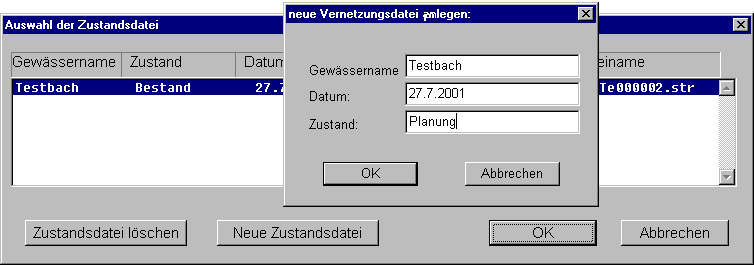
\includegraphics[width=0.9\textwidth]{NeuerZustand}
   \caption{Anlegen und \"{O}ffnen einer neuen Zustandsdatei}
   \label{Einstieg Abb ZustandsdateiNeu}
\end{figure}
S\"{a}mtliche weiteren Arbeiten beziehen sich nun auf die gew\"{a}hlte Zustandsdatei. Bevor weitere Arbeitsschritte ausgef\"{u}hrt
werden k\"{o}nnen, m\"{u}ssen immer zuerst ein Projekt und eine Zustandsdatei ge\"{o}ffnet sein.


\subsection{Zustand l\"{o}schen}

Ebenso wie Sie eine Zustandsdatei \"{o}ffnen k\"{o}nnen, ist es m\"{o}glich in der Maske \dialog{Auswahl der Zustandsdatei} durch
Markieren der entsprechenden Datei und Dr\"{u}cken der Schaltfl\"{a}che \schalter{Zustandsdatei l\"{o}schen} eine Zustandsdatei aus
dem Projektverzeichnis zu entfernen. Es erfolgt eine Abfrage, ob Sie sich sicher sind, da{\ss} die entsprechende Datei zu
l\"{o}schen ist. Ferner werden Sie vor die Frage gestellt, ob Profile, die nur in dieser einen Zustandsdatei referenziert
sind, auch physisch gel\"{o}scht werden sollen.
\begin{hinweis}
   L\"{o}schen Sie Profile, die nicht mehr ben\"{o}tigt werden m\"{o}glichst sofort, um \afz{Dateileichen} auf Ihrem Rechner zu vermeiden.
   Ein sp\"{a}teres L\"{o}schen aus der Oberfl\"{a}che heraus ist nur noch \"{u}ber eine Zustandsdatei m\"{o}glich, d.h. Sie m\"{u}ssen zun\"{a}chst
   eine neue Zustandsdatei erstellen, die Profile aufnehmen und wieder l\"{o}schen. Andererseits haben Sie aber die M\"{o}glichkeit,
   Profile physisch zu erhalten, um sie sp\"{a}ter wieder einer neuen Zustandsdatei zuzuordnen. Wenn die Profile noch in anderen
   Vernetzungsdateien referenziert sind, k\"{o}nnen sie nicht physisch gel\"{o}scht werden.
\end{hinweis}

\subsection{Beispiel Zustandsdatei anlegen}
\label{Einstieg Subsec BeispielZustandsdatei}

Legen Sie innerhalb des Projektes \afz{Beispiel} die Zustandsdatei \afz{Testbach} f\"{u}r die Bestandsplanung an. \"{O}ffnen Sie
dazu zun\"{a}chst das Projekt (siehe Abschnitt~\ref{Einstieg Subsec ProjektOeffnen}). \"{U}ber die Schaltfl\"{a}che \schalter{Neue
Zustandsdatei} in der Maske \dialog{Auswahl der Zustandsdatei} gelangen Sie in den Dialog \dialog{Neue Vernetzungsdatei
anlegen}, hier tragen Sie ein:
\begin{quote}
   \begin{tabular}{ll}
      Gew\"{a}ssername:  &  \beisp{Testbach} \\
      Datum:         &  \beisp{24.07.2001} \\
      Zustand:       &  \beisp{Bestand}
   \end{tabular}
\end{quote}
Nach der Best\"{a}tigung \schalter{OK} erscheint die neue Zustandsdatei in der in der Maske \dialog{Auswahl der
Zustandsdatei}.


\clearpage
%%%%%%%%%%%%%%%%%%%%%%%%%%%%%%%%%%%%%%%%%%%%%%%%%%%%%%%%%%%%%%%%%%%%%%%%%%%%%%%%%%%%%%%%%%%%%%%%%%%%%%%%%%%%%%%%%%%%%%%%%%%%
\section{Profildateien bearbeiten}
%%%%%%%%%%%%%%%%%%%%%%%%%%%%%%%%%%%%%%%%%%%%%%%%%%%%%%%%%%%%%%%%%%%%%%%%%%%%%%%%%%%%%%%%%%%%%%%%%%%%%%%%%%%%%%%%%%%%%%%%%%%%
Nachdem Sie eine Zustandsdatei ge\"{o}ffnet haben, gelangen Sie automatisch in eine Maske \dialog{Erfas\-sung/Edi\-tierung der
Zustandsdatei}, was alternativ auch \"{u}ber den Men\"{u}punkt \menu{\marrow Z\underline{u}\-stand \marrow \underline{E}ditieren
der Zustandsdatei/Profile} m\"{o}glich ist. Mit Hilfe dieser Maske k\"{o}nnen Sie:
\begin{itemize}
   \item Neue Profile anlegen
   \item Profile aus einer anderen Zustandsdatei aufnehmen
   \item Profile l\"{o}schen
\end{itemize}
Zur Bearbeitung der Profile stehen Ihnen ein alphanumerischer und ein grafisch-interaktiver Editor zur Verf\"{u}gung.
\begin{figure}[hpt]
   \centering
   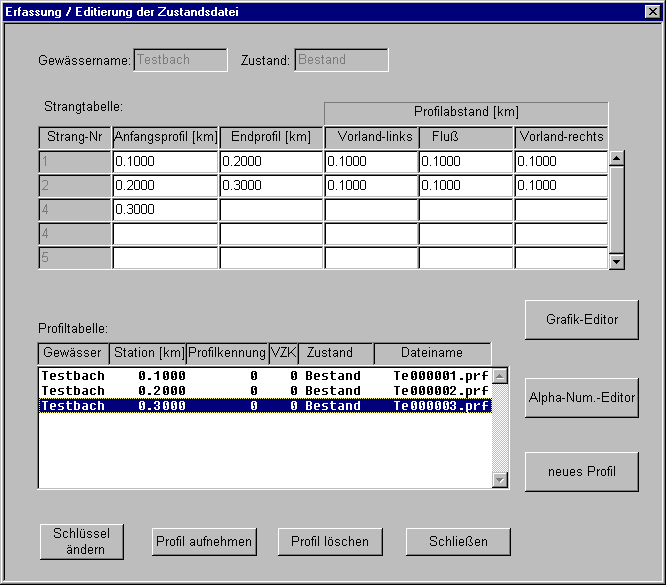
\includegraphics[width=1.0\textwidth]{ErfassungEditierungZustandsdatei}
   \caption{Die Maske zum Erfassen und Editieren der Zustandsdatei}
   \label{Einstieg Abb ErfassungEditierungZustandsdatei}
\end{figure}


\subsection{Ein neues Profil anlegen}
\label{Einstieg Subsec ProfilAnlegen}

Sofern Sie eine neue Zustandsdatei angelegt haben, enth\"{a}lt der Dialog \dialog{Erfas\-sung/Edi\-tierung der Zustandsdatei}
keine Eintr\"{a}ge. Die Strangtabelle im oberen Teil der Dialogmaske und die Profiltabelle im unteren Teil, die automatisch
beim Anlegen eines Profils ausgef\"{u}llt werden, sind leer. In diesem Fall k\"{o}nnen Sie entweder \"{u}ber die Option
\schalter{Profil aufnehmen} bereits existierende Profile (im BCE-Format) in den Zustand \"{u}bernehmen, oder aber ein neues
Profil anlegen. In letzterem Fall w\"{a}hlen Sie die Schaltfl\"{a}che \schalter{Neues Profil}. Es erscheint eine Maske, die Sie
zur Angabe des Profilschl\"{u}ssels auffordert, \"{u}ber den die neue Profildatei referenziert werden soll
(Abbildung~\ref{Einstieg Abb Profilschluessel}).
\begin{figure}[ht]
   \centering
   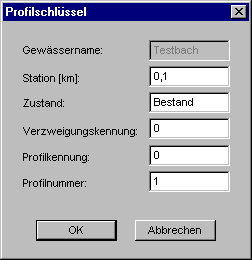
\includegraphics[width=0.4\textwidth]{Profilschluessel}
   \caption{Eingabemaske f\"{u}r den Profilschl\"{u}ssel}
   \label{Einstieg Abb Profilschluessel}
\end{figure}

Der Profilschl\"{u}ssel setzt sich aus dem Gew\"{a}ssernamen (es wird der Name \"{u}bernommen, den Sie der entsprechenden
Zustandsdatei zugeordnet haben), der Stationsangabe (in $\mathrm{km}$), dem Profilzustand (es wird der Zustand der
Verkn\"{u}pfungsdatei vorgeschlagen) sowie der Verzweigungs- und Profilkennung zusammen. Innerhalb eines Projektes darf ein
Profilschl\"{u}ssel nur einmal vorkommen, d.h. es k\"{o}nnen keine Profile mit identischem Gew\"{a}ssernamen, Profilzustand, sowie
der gleichen Verzweigungs- und Profilkennung an einer Station existieren.

Standardm\"{a}{\ss}ig werden Ihnen bei der Verzweigungs- und Profilkennung die Werte $0$ vorgeschlagen (keine Verzweigung,
keine Mehrfeldbr\"{u}cke). Zus\"{a}tzlich k\"{o}nnen sie in dem Feld \dialog{Profilnummer} eine pers\"{o}nliche Identifikation f\"{u}r das
Profil eingeben, die Ihnen z.B. die Zuordnung zum entsprechenden Aufma{\ss} erleichtert. Die Stationierungsrichtung ist
nicht festgelegt. Es wird jedoch empfohlen, im Sinne des Gew\"{a}sserverzeichnisses~NRW grunds\"{a}tzlich von der M\"{u}ndung
($\mathrm{km}~0$) in Richtung Quelle aufsteigend zu stationieren.

Die Profile k�nnen in beliebiger Reihenfolge eingegeben werden. Die Sortierung erfolgt au\-to\-ma\-tisch anhand der Stationierung in aufsteigender Reihenfolge. Soll umgekehrt sta\-tio\-niert wer\-den, ist unter \menu{\marrow Extras \marrow Optionen} bei der Sortierung der Strangtabelle \schalter{r�ckw�rts} zu w�h\-len. Nach der Eingabe des Profilschl�ssels und Best�tigung mit \schalter{OK} gelangen Sie auto\-ma\-tisch in den alpha\-nu\-me\-ri\-schen Editor (Abbildung~\ref{Einstieg Abb AlphanumerischerEditor}).

\subsection{Dateneingabe im alphanumerischen Editor}

Aus dem Dialog \dialog{Erfassung/Editierung der Zustandsdatei} gelangen Sie \"{u}ber die Schaltfl\"{a}che
\schalter{Alpha-Num.-Editor} in den alphanumerischen Editor (Abbildung~\ref{Einstieg Abb AlphanumerischerEditor}). Beim
Anlegen eines neuen Profilschl\"{u}ssels wird dieser automatisch ge\"{o}ffnet. Mit seiner Hilfe lassen sich profilbezogene Daten
eingeben und ver\"{a}ndern.

In der rechten oberen Ecke werden Ihnen die wichtigsten Schl\"{u}sseldaten des Profils, wie z.B. Gew\"{a}ssername und
Stationswert angezeigt. Darunter finden Sie ein Editierfeld, in dem Sie einen Kommentar speziell zu dem aktuellen
Profil eingeben k\"{o}nnen. In der linken Bildh\"{a}lfte befindet sich eine Tabelle, in der die Werte f\"{u}r den jeweils in dem
Listenfeld der rechten Bildh\"{a}lfte (unter dem Kommentar) angezeigten Datensatz eingegeben werden k\"{o}nnen. Wenn Sie noch
keine anderen sogenannten Datenblocktypen (siehe Abschnitt~\ref{Einstieg Subsec Grafikeditor}) angelegt haben,
erscheint beim Klicken auf den Pfeil des Listenfeldes nur die Gel\"{a}ndeh\"{o}he.
\begin{figure}[hbt]
   \centering
   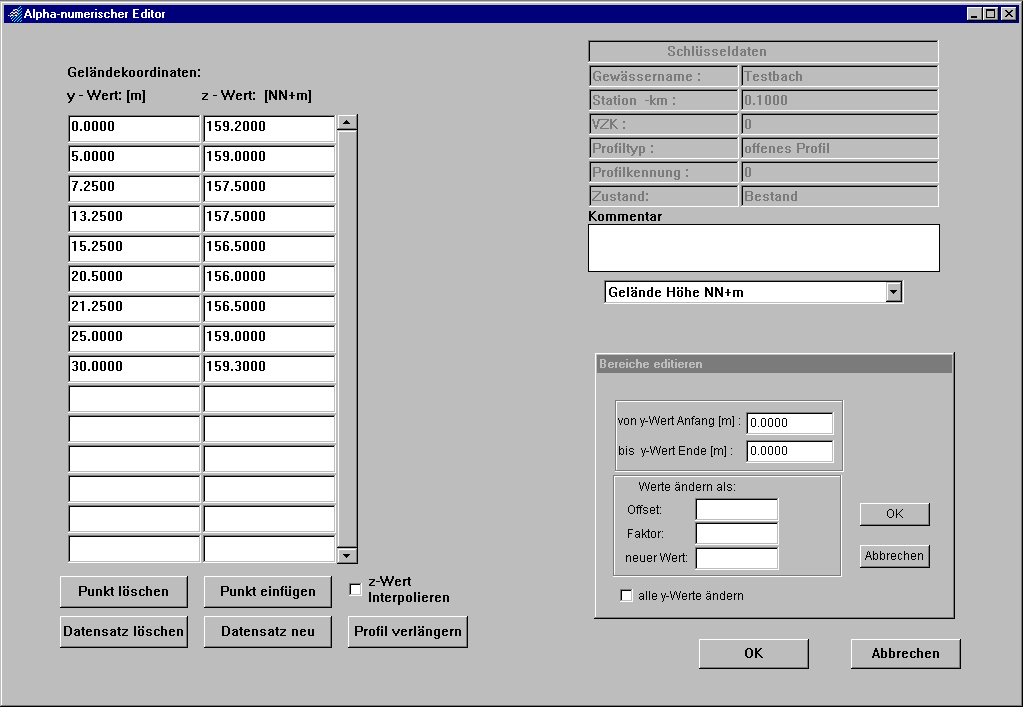
\includegraphics[width=1.0\textwidth]{AlphanumerischerEditor}
   \caption{Der alphanumerische Editor}
   \label{Einstieg Abb AlphanumerischerEditor}
\end{figure}

Bei Aufruf des alphanumerischen Editors wird standardm\"{a}{\ss}ig zun\"{a}chst der Datensatz Gel\"{a}ndeh\"{o}he angezeigt. Die
Gel\"{a}ndeh\"{o}he mu{\ss} in jedem Fall (auch bei Sonderprofilen wie z.B. Durchl\"{a}ssen) eingeben werden und stellt den Bezug f\"{u}r
alle weiteren Datens\"{a}tze dar. Bei dem Datensatz Gel\"{a}ndeh\"{o}he besteht das Spreadsheet aus zwei Spalten f\"{u}r die
Gel\"{a}ndekoordinaten des Profils.

Die $y$-Werte bezeichnen die Distanz der Me{\ss}- bzw. Profilpunkte zu einem Referenzpunkt im Querprofil. Negative Werte sind
m\"{o}glich. Zur Vermeidung von falschen Zuordnungen sollten die Querprofile grunds\"{a}tzlich in Flie{\ss}richtung gesehen
aufgetragen werden. Der allgemein \"{u}blichen Konvention entsprechend erfolgt die Zuordnung von links nach rechts in
Flie{\ss}richtung. Die $z$-Werte geben die Gel\"{a}ndeh\"{o}he in [NN+m] an den jeweiligen Profilpunkten wieder.

Maximal k\"{o}nnen bis zu 500~Profilpunkte in einem Querprofil angelegt werden. Bei \"{a}lteren Versionen des Berechnungsprogramms
kann die Anzahl von Profilpunkten aus Speicherplatzgr\"{u}nden noch auf 50 beschr\"{a}nkt sein. Eine Profildatei besteht aus
mindestens zwei Gel\"{a}ndekoordinaten.
\begin{hinweis}
   Anstelle der Gel\"{a}ndeh\"{o}he in [NN+m] kann auch ein anderes H\"{o}henbezugssystem gew\"{a}hlt werden, z.B.
   [m+HN]. Ist ein Anschlu{\ss} an ein H\"{o}henbezugssystem nicht vorhanden, so w\"{a}hlen Sie sich einen Referenzpunkt und
   weisen ihm eine fiktive H\"{o}henangabe zu.
\end{hinweis}

Die Tabellenwerte im Spreadsheet des alphanumerischen Editors k\"{o}nnen vom Benutzer direkt editiert werden. Indem der
Mauszeiger auf das entsprechende Editierfeld bewegt und ein neuer Wert eingegeben wird, k\"{o}nnen die angezeigten Daten
ge\"{a}ndert bzw. neue Daten eingegeben werden. \"{U}ber die Tabulator- und Entertaste ist ein Springen zwischen den Editierfeldern
m\"{o}glich. Punkt oder Komma machen bei der Dateneingabe keinen Unterschied.

Die $y$- und zugeh\"{o}rigen $z$-Werte werden in der Reihenfolge gespeichert, wie Sie sie im Spreadsheet eingegeben haben.
Bei Normalprofilen ist eine Sortierung der $y$-Werte in aufsteigender Reihenfolge zu gew\"{a}hrleisten. Lediglich bei
Profilen mit R\"{u}ckspr\"{u}ngen kann davon abgewichen werden\footnote{Zur besseren Kontrolle werden Profilpunkte an R�ckspr�ngen und senkrechten W�nden im Textfeld rot markiert.}. \"{U}ber die Schaltfl\"{a}chen \schalter{Punkt einf\"{u}gen} und
\schalter{Punkt l\"{o}schen} wird vor dem Wert, auf dem sich der Cursor befindet, ein Punkt eingef\"{u}gt, bzw. der Wert des
aktuellen Editierfeldes gel\"{o}scht.

Es ist auch m\"{o}glich einen Punkt interpolieren zu lassen. Dazu f\"{u}gen Sie zun\"{a}chst einen Punkt ein, markieren dann die
Checkbox \checkbox{z-Wert interpolieren}, geben den $y$-Wert ein und klicken in das Feld f\"{u}r die $z$-Werte. Es erscheint
die linear interpolierte Gel\"{a}ndeh\"{o}he an der Stelle des $y$-Wertes.
\begin{hinweis}
   Vermeiden Sie die Eingabe von genau vertikalen W\"{a}nden, da sich dort in der Regel auch die Trennfl\"{a}chen befinden. Diese
   werden dann unter Umst\"{a}nden vom Programm nicht eindeutig zugeordnet.
\end{hinweis}

Um neue Datenblocktypen f\"{u}r das Profil anzulegen, w\"{a}hlen Sie den Schalter \schalter{Datensatz neu}. Zu empfehlen ist es,
die Gel\"{a}ndeh\"{o}he im alphanumerischen Editor einzugeben, diesen mit \schalter{OK} (Speichern) zu verlassen und anschlie{\ss}end
in den Grafik\-editor zu wechseln, um dort weitere Datens\"{a}tze anzulegen. Sie k\"{o}nnen aber auch alle Eingaben im
alphanumerischen Editor vornehmen.
\begin{hinweis}
   Kontrollieren Sie die Profilform indem Sie nach der Dateneingabe in den Grafikeditor wechseln.
   Sie beugen damit Tippfehlern als auch Fehler in der Eingabereihenfolge der Punkte vor.
\end{hinweis}
Haben Sie vor dem Verlassen des Editors die Datens\"{a}tze \afz{Rauheit}, \afz{Trennfl\"{a}chen} und \afz{durchstr\"{o}mte Bereiche}
nicht angelegt, so werden Sie vor die Frage gestellt, ob \wspwin{} diese automatisch f\"{u}r Sie erstellen soll. Die
Trennfl\"{a}chen und die Grenzen des durchstr\"{o}mten Bereiches werden bei der automatischen Generierung am \"{a}u{\ss}eren Rand Ihres
Profils eingef\"{u}gt. Die Rauheit kann nur automatisch erstellt werden, wenn zuvor unter dem Men\"{u} \menu{\marrow
E\underline{x}tras \marrow \underline{O}ptionen} eine automatische Generierung der Rauheit vereinbart wurde (siehe hierzu Abschnitt~\ref{Installation Subsec Standardeinstellungen}).


\subsection{Dateneingabe im Grafikeditor}
\label{Einstieg Subsec Grafikeditor}

Neben dem Editieren der Profildateien im alphanumerischen Editor existiert in \wspwin{} auch eine wesentlich einfachere
und anschaulichere M\"{o}glichkeit Eingabewerte zu editieren, n\"{a}mlich der Grafikeditor. Der grafische Editor wird wie der
alphanumerische Editor aus dem Dialogfenster \dialog{Erfassung/Editierung der Zustandsdatei} heraus aufgerufen.

Sobald Sie den grafischen Editor aufgerufen haben, erhalten Sie eine grafische Darstellung der Gel\"{a}ndeh\"{o}he f\"{u}r Ihr zuvor
markiertes Profil. Daneben finden Sie in der linken Bildmitte noch einmal die wichtigsten Schl\"{u}sseldaten ihres Profils und
ein Editierfeld f\"{u}r einen beliebigen Kommentartext, sowie in der rechten oberen Ecke, entsprechend des alphanumerischen
Editors, eine editierbare Tabelle der $y$- und $z$-Werte. Wie beim alphanumerischen Editor k\"{o}nnen Sie auch hier \"{u}ber ein
Listenfeld unterschiedliche Datenblocktypen darstellen lassen und zwar sowohl in der Tabelle wie auch in der Grafik.
Standardm\"{a}{\ss}ig wird zun\"{a}chst nur die Gel\"{a}ndeh\"{o}he angezeigt.

Der grafisch-interaktive Editor setzt sich dementsprechend aus einem alphanumerischen Editor und einem grafischen Editor
zusammen, wobei \"{A}nderungen in einem der beiden Editoren eine direkte Aktualisierung des jeweils anderen Editors zur Folge
haben. Sobald Sie einen Zahlenwert im alphanumerischen Editor \"{a}ndern und das Editierfeld verlassen, wird die Grafik
aktualisiert und Sie k\"{o}nnen das Resultat anschaulich bewerten. Umgekehrt k\"{o}nnen Sie direkt in der Grafik f\"{u}r jeden
Profilpunkt, der durch eine senkrechte Linie gekennzeichnet ist, \"{A}nderungen vornehmen.
\begin{figure}
   \centering
   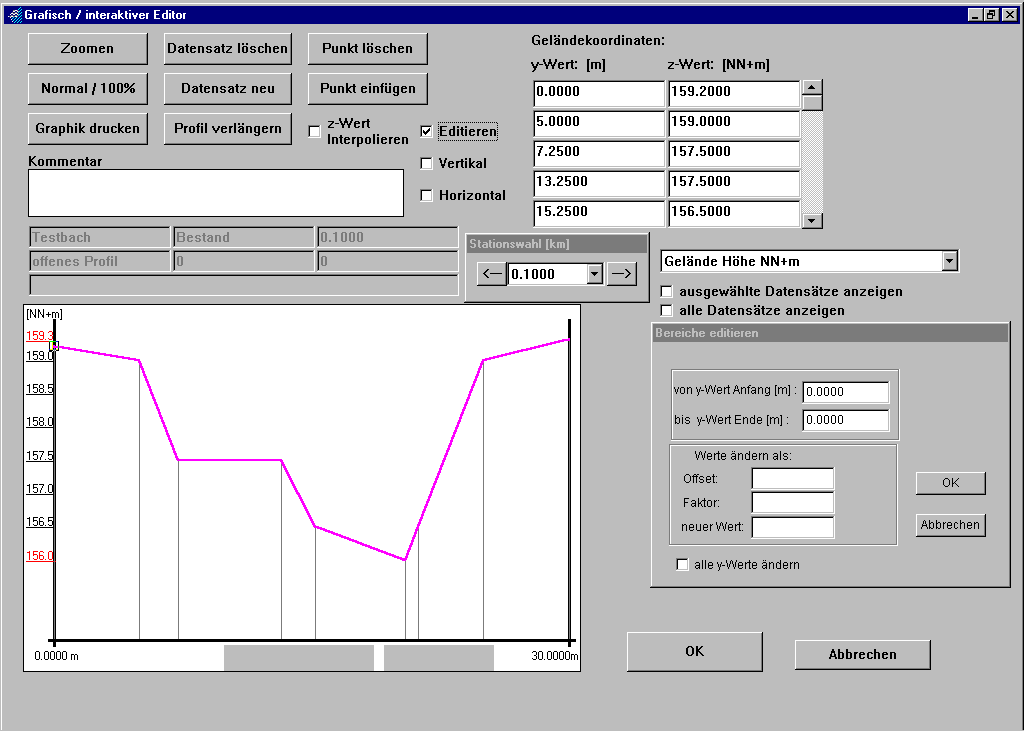
\includegraphics[width=1.0\textwidth]{Grafikeditor}
   \caption{Der Grafikeditor}
   \label{Einstieg Abb Grafikeditor}
\end{figure}

Sobald Sie die Maus in die Grafik bewegen, wandelt sich der Mauszeiger in ein Fadenkreuz um. Unter der Grafik erscheinen
die $y$- und $z$-Koordinaten f\"{u}r den Punkt, an dem sich das Fadenkreuz gerade befindet. Ein K\"{a}stchen \"{u}ber dem Profilpunkt
in der Grafik zeigt Ihnen gleichzeitig Ihre aktuelle Position im alphanumerischen Editor. Sobald Sie sich im
alphanumerischen Editor bewegen, wandert auch das K\"{a}stchen. Damit behalten Sie den \"{U}berblick \"{u}ber beide Editoren und
k\"{o}nnen Ver\"{a}nderungen im jeweils anderen Editor unmittelbar wahrnehmen. Die Schaltfl\"{a}chen \schalter{Punkt einf\"{u}gen},
\schalter{Punkt l\"{o}schen}, \schalter{Datensatz neu}, \schalter{Datensatz l\"{o}schen} sowie \schalter{Profil verl\"{a}ngern}
entsprechen denen des alphanumerischen Editors. Daneben finden Sie ganz links die Funktionen \schalter{Zoomen},
\schalter{Normal/100\%} und \schalter{Grafik drucken}.

Um einen Ausschnitt des Profils vergr\"{o}{\ss}ert darzustellen w\"{a}hlen sie \schalter{Zoomen} und markieren mit gedr\"{u}ckter linker
Maustaste den Grafikausschnitt, den sie vergr\"{o}{\ss}ert betrachten m\"{o}chten. Mit \schalter{Normal/100\%} stellen Sie den
urspr\"{u}nglichen Zustand wieder her. Neben der Gel\"{a}ndeh\"{o}he sind weitere Datenblocktypen in \wspwin{} verf\"{u}gbar.
Tabelle~\ref{Einstieg Tab GrafischeDatenblocktypen} gibt einen \"{U}berblick, welche Datenblocktypen grafisch dargestellt und
welche zus\"{a}tzlich grafisch-interaktiv bearbeitet werden k\"{o}nnen. Um sich mehrere Datenblocktypen in der Grafik anzeigen zu
lassen markieren Sie die Option \checkbox{ausgew\"{a}hlte Datens\"{a}tze anzeigen} und w\"{a}hlen daraufhin die gew\"{u}nschten Datens\"{a}tze
aus dem Listenfeld aus. Die Option \checkbox{alle Datens\"{a}tze anzeigen} f\"{u}gt alle darstellbaren Datenbl\"{o}cke in die Grafik
ein.
\begin{table}
   \centering
   \input{Einstieg/tab/Datenblocktypen.tab}
   \caption{Grafische Bearbeitung der Datenblocktypen}
   \label{Einstieg Tab GrafischeDatenblocktypen}
\end{table}

\"{A}nderungen der Gel\"{a}ndeh\"{o}he k\"{o}nnen in der Grafik schnell und unkompliziert dadurch vorgenommen werden, da{\ss} Sie sich,
nachdem Sie die Kontrollk\"{a}stchen \checkbox{Editieren} und \checkbox{Horizontal} oder \checkbox{Vertikal} aktiviert haben,
mit der Maus an den gew\"{u}nschten Profilpunkt bewegen und bei gedr\"{u}ckter linker Maustaste die Gel\"{a}ndekontur verziehen. Der
alphanumerische Editor wird sodann aktualisiert. Beachten Sie, da{\ss} die grafische Darstellung grunds\"{a}tzlich an den h\"{o}chsten
und niedrigsten Gel\"{a}ndeh\"{o}hen orientiert ist, was zu einer starken \"{U}berh\"{o}hung und nicht ma{\ss}st\"{a}blichen Darstellungen f\"{u}hrt.
Zwischen einzelnen Profilen k\"{o}nnen Sie ohne den Grafik-Editor zu verlassen durch Klicken der Pfeiltasten auf dem
Listenfeld \dialog{Stationswahl} und Auswahl des entsprechenden Profils springen.


\subsection{Bereiche editieren}
\label{Einstieg Subsec BereicheEditieren}

Eine weitere Hilfe f\"{u}r die Dateneingabe der Gel\"{a}ndeh\"{o}hen im alphanumerischen und im grafischen Editor bietet der Dialog
\dialog{Bereiche editieren}. Hier k\"{o}nnen mehrere Werte gleichzeitig ge\"{a}ndert werden. Besonders vorteilhaft ist dies bei
regelm\"{a}{\ss}igen Gerinnen in denen sich nur die Gel\"{a}ndeh\"{o}he \"{a}ndert.
\begin{figure}[hbt]
   \centering
   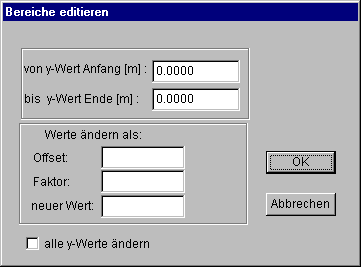
\includegraphics[width=0.5\textwidth]{BereicheEditieren}
   \caption{Dialogfenster zum Editieren von Bereichen}
   \label{Einstieg Abb BereicheEditieren}
\end{figure}

Legen Sie dazu zun\"{a}chst den zu editierenden Bereich mit Hilfe der Felder $y$-Wert Anfang und Ende fest oder aktivieren Sie
das Kontrollfeld \checkbox{alle y-Werte \"{a}ndern}. Im Grafikeditor kann der zu \"{a}ndernde Bereich auch durch verschieben der
Maus \"{u}ber der Grafik bei gedr\"{u}ckter linker Maustaste festgelegt werden. Die Felder Offset, Faktor und neuer Wert bewirken
folgendes:
\begin{description}
   \item[Offset:]
      Der hier eingegebene Wert wird zu den Gel\"{a}ndeh\"{o}hen des ausgew\"{a}hlten Bereiches abh\"{a}ngig vom Vorzeichen addiert oder
      subtrahiert.
   \item[Faktor:]
      Es erfolgt eine Multiplikation aller Gel\"{a}ndeh\"{o}hen im ausgew\"{a}hlten Bereich mit dem angegebenen Wert.
   \item[Neuer Wert:]
      Alle Gel\"{a}ndeh\"{o}hen des ausgew\"{a}hlten Bereichs werden auf den hier eingegebenen Zahlenwert ge\"{a}ndert.
\end{description}
Bitte beachten Sie, da{\ss} die Funktionen nur einzeln ausgef\"{u}hrt werden k\"{o}nnen.


\subsection{Neue Datens\"{a}tze anlegen}

Mit dem Schalter \schalter{Datensatz neu} aus dem alphanumerischen oder Grafikeditor heraus haben Sie die M\"{o}glichkeit,
neben der Gel\"{a}ndeh\"{o}he auch andere Datenblocktypen in das Profil aufzunehmen. Ein Normalprofil besteht immer mindestens
aus den Datens\"{a}tzen
\begin{itemize}
   \item Gel\"{a}ndeh\"{o}he
   \item Rauheit
   \item Trennfl\"{a}chen
   \item Durchstr\"{o}mte Bereiche
\end{itemize}
die mit Hilfe von \wspwin{} beim Verlassen des Editors auch automatisch generiert werden k\"{o}nnen.

Beim Neuanlegen eines Datensatzes erscheint zun\"{a}chst wiederum ein Listenfeld, aus dem Sie einen Datenblock w\"{a}hlen k\"{o}nnen.
Anschlie{\ss}end sind Werte (in Abh\"{a}ngigkeit vom Typ) zum neu eingef\"{u}gten Datenblock einzugeben. Eine \"{U}bersicht \"{u}ber die
vorhandenen Datensatztypen gibt Tabelle~\ref{Einstieg Tab GrafischeDatenblocktypen} in Abschnitt~\ref{Einstieg Subsec
Grafikeditor}.

Ein Datensatz kann inklusive seiner Werte \"{u}ber den Schalter \schalter{Datensatz l\"{o}schen} wieder aus der Profildatei
entfernt werden. Die Dateneingabe f\"{u}r die einzelnen Datens\"{a}tze sind in den nachfolgenden Kapiteln n\"{a}her erl\"{a}utert.


\subsection{Rauheit eingeben}
\label{Einstieg Subsec Rauheit}

Rauheiten k\"{o}nnen in \wspwin{} wahlweise als \autor{Darcy-Weisbach}-Rauheiten ($k_S$-Werte in [$\mathrm{m}$]) oder
\autor{Manning-Strickler}-Rauheiten ($k_{ST}$-Werte in [$\mathrm{m^{1/3}/s}$]) eingegeben werden. Sobald Sie \"{u}ber den
Schalter \schalter{Datensatz neu} den Datenblocktyp Rauheit eingef\"{u}gt haben (entweder als $k_S$- oder $k_{ST}$-Werte --
die Datens\"{a}tze schlie{\ss}en sich gegenseitig aus), \"{o}ffnet sich im Spreadsheet des alphanumerischen oder grafischen Editors
neben den $y$-und $z$-Werten der Gel\"{a}ndeh\"{o}he eine 3.~Spalte, in der Sie den einzelnen Profilpunkten Rauheiten zuordnen
k\"{o}nnen.
\begin{hinweis}
   Beachten Sie bei der Festlegung des Datenblocktyps f\"{u}r die Rauheit, da{\ss} dieser die Grundlage f\"{u}r die Auswahl der
   Berechnungsmethode darstellt. Es ist z.B. nicht m\"{o}glich die Berechnung nach dem Flie{\ss}gesetz von \autor{Manning-Strickler}
   auf Basis der \autor{Darcy-Weisbach}'schen Rauheiten durchzuf\"{u}hren.
\end{hinweis}

Haben Sie den Datensatz Rauheit eben erst neu angelegt, brauchen nur die Profilpunkte besetzt werden, an denen eine
\"{A}nderung der Rauheit gegen\"{u}ber den vorherigen Profilpunkten stattfindet. Alle nachfolgenden Profilpunkte werden beim
Speichern der Datei \"{u}ber \schalter{OK} mit dem jeweils davor besetzten Wert aufgef\"{u}llt. Sind die Rauheiten im
Spread\-sheet bereits durch den Wert $0,00$ vorbelegt (z.B. bei einer automatischen Generierung der Rauheiten nach
Abschnitt~\ref{Installation Subsec Standardeinstellungen}), so m\"{u}ssen sie alle Werte neu angeben.

Neben der alphanumerischen Eingabe k\"{o}nnen die Rauheiten auch grafisch-interaktiv ver\"{a}ndert werden. W\"{a}hlen Sie
dazu zun\"{a}chst den Datenblocktyp Rauheit aus dem Listenfeld. Markieren Sie nun mit gedr\"{u}ckter linker Maustaste den
Bereich in der Grafik, den Sie ver\"{a}ndern m\"{o}chten. Es erscheint ein Dialogfenster mit dem Sie wiederum Bereiche im
Querprofil anpassen k\"{o}nnen. Zus\"{a}tzlich zu den in Abschnitt~\ref{Einstieg Subsec BereicheEditieren} angegebenen
Funktionen enth\"{a}lt der Dialog eine Schaltfl\"{a}che \schalter{Datenbank}. Der Umgang mit der Rauheitsdatenbank wird in
Abschnitt~\ref{Fortgeschrittene Subsec Rauheitsdatenbank} n\"{a}her erl\"{a}utert.

Beachten Sie, dass eine Ver�nderung der Trennfl�chen eine �nderung der Rauheitswerte nach sich ziehen kann 	(siehe Abschnitt~\ref{sec:einstieg:profildaten:trennflaechen}).

\begin{table}[hbtp]
   \centering
   \input{Einstieg/tab/Einzelrauheiten.tab}
   \caption{Typische Einzelrauheiten}
   \label{Einstieg Tab Einzelrauheiten}
\end{table}

\subsection{Trennfl\"{a}chen definieren}
\label{sec:einstieg:profildaten:trennflaechen}

Die verwendeten Bestimmungsgleichungen f\"{u}r die Querschnittswerte und die hydraulischen Kenngr\"{o}{\ss}en sind auf dreifach
gegliederte Querschnitte (Abbildung~\ref{Einstieg Abb Teilabflussflaechen}) abgestimmt (linkes Vorland, Flu{\ss}schlauch,
rechtes Vorland). Die Teilabflu{\ss}fl\"{a}chen werden als Stromr\"{o}hren mit horizontalem Wasserspiegel gleicher H\"{o}he aufgefa{\ss}t.
\begin{figure}[hbt]
   \begin{minipage}{1.0\textwidth}
      \centering
      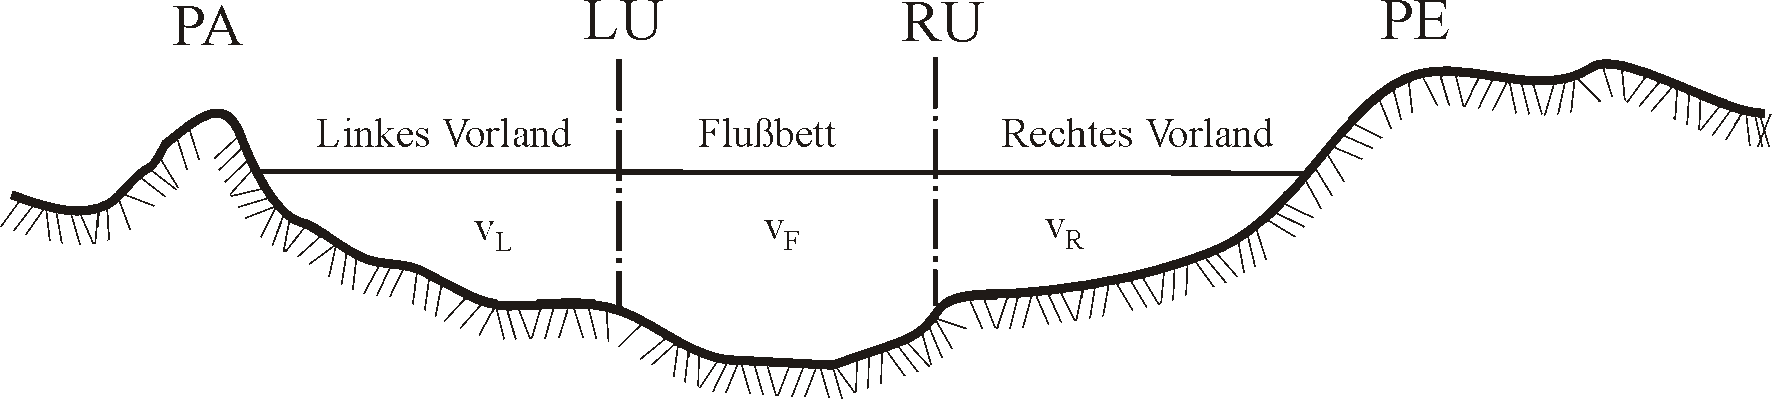
\includegraphics[width=1.0\textwidth]{Trennflaechen}
      \caption{Teilabflu{\ss}fl\"{a}chen eines Flie{\ss}querschnitts}
      \label{Einstieg Abb Teilabflussflaechen}
      \vspace{12pt}
   \end{minipage}
   \begin{minipage}{1.0\textwidth}
      \centering
      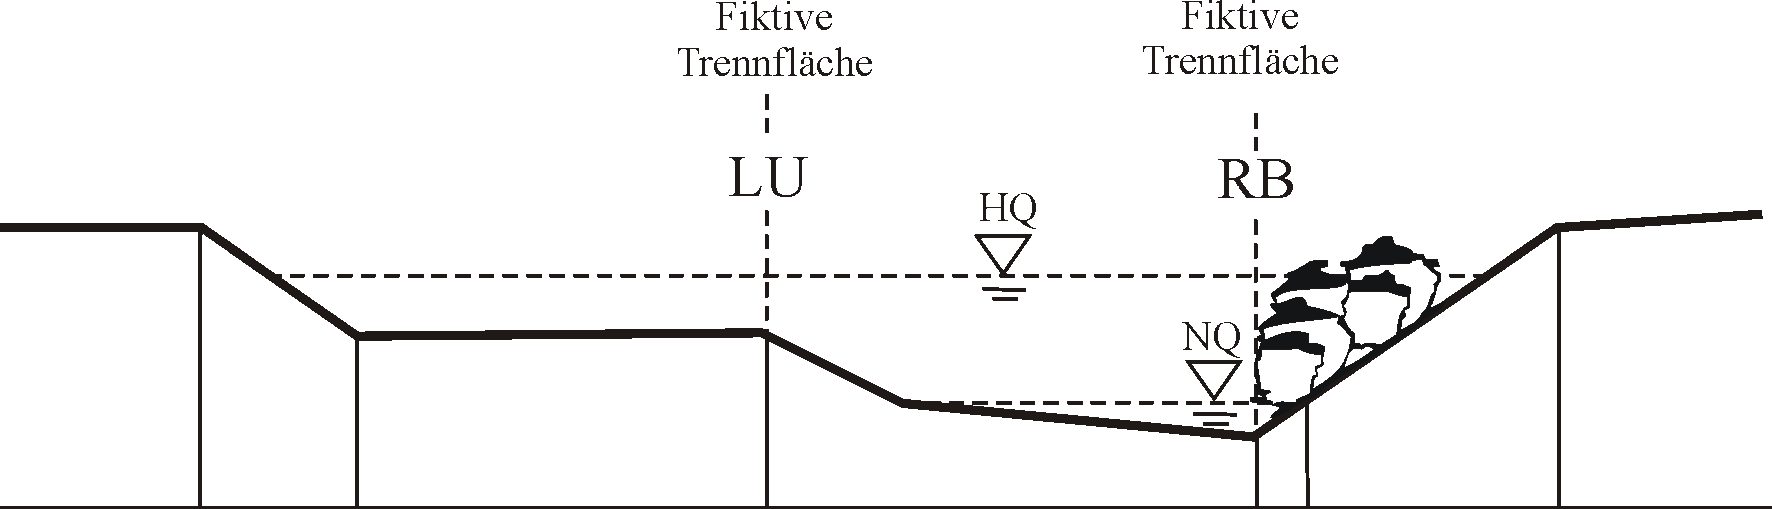
\includegraphics[width=1.0\textwidth]{TrennflaechenBewuchs}
      \caption{Lage der Trennfl\"{a}che bei B\"{o}schungsbewuchs}
      \label{Einstieg Abb Boeschungsbewuchs}
   \end{minipage}
\end{figure}
Die Gliederung des Querschnitts in Teilabflu{\ss}fl\"{a}chen wird durch die Definition der Lage fiktiver Trennfl\"{a}chen festgelegt.
\begin{quote}
   \begin{labeling}[:]{RU (Rechtes Ufer)}
      \item[PA (Profilanfang)]  Anfang des abflu{\ss}wirksamen Querschnitts \newline (linke Grenze des durchstr\"{o}mten Bereichs)
      \item[LU (Linkes Ufer) ]  Grenzpunkt zwischen linkem Vorland und Flu{\ss}schlauch (linke Trennfl\"{a}che)
      \item[RU (Rechtes Ufer)]  Grenzpunkt zwischen Flu{\ss}schlauch und rechtem Vorland (rechte Trennfl\"{a}che)
      \item[PE (Profilende)  ]  Ende des abflu{\ss}wirksamen Querschnitts \newline (rechte Grenze des durchstr\"{o}mten Bereichs)
   \end{labeling}
\end{quote}
Bei Profilen mit Bewuchs ist zu beachten, da{\ss} bei bepflanzten B\"{o}schungen jeweils der B\"{o}schungsfu{\ss}punkt als Grenzpunkt
zwischen Flu{\ss}schlauch und Vorland zu definieren ist (Abbildung~\ref{Einstieg Abb Boeschungsbewuchs}).
\begin{figure}[hbt]
   \centering
   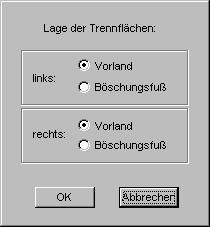
\includegraphics[width=0.35\textwidth]{LageTrennflaechen}
   \caption{Festlegen der Lage der Trennfl\"{a}chen}
   \label{Einstieg Abb LageTrennflaechen}
\end{figure}

Nachdem Sie einen neuen Datensatz \afz{Trennfl\"{a}chen} \"{u}ber den Schalter \schalter{Datensatz neu} angelegt haben, erscheint
ein Sonderdialog, in dem zun\"{a}chst als linker und rechter Profilpunkt f\"{u}r die Trennfl\"{a}chen die beiden \"{a}u{\ss}ersten
Profilpunkte angegeben sind. Diese Werte k\"{o}nnen Sie, je nachdem wo die Trennfl\"{a}chen positioniert werden sollen, mit
anderen $y$-Werten \"{u}berschreiben. Auch beim automatischen Anlegen der Trennfl\"{a}chen werden diese immer nach au{\ss}en gesetzt.

Per Voreinstellung markieren die Trennfl\"{a}chen den \"{U}bergang von der B\"{o}schung auf das Vorland. \"{U}ber den Schalter
\schalter{Lage...} haben Sie aber auch die M\"{o}glichkeit die Lage bei Bewuchs (Abbildung~\ref{Einstieg Abb
Boeschungsbewuchs}) rechts oder links an den B\"{o}schungsfu{\ss} zu legen.
\begin{figure}[hbt]
   \centering
   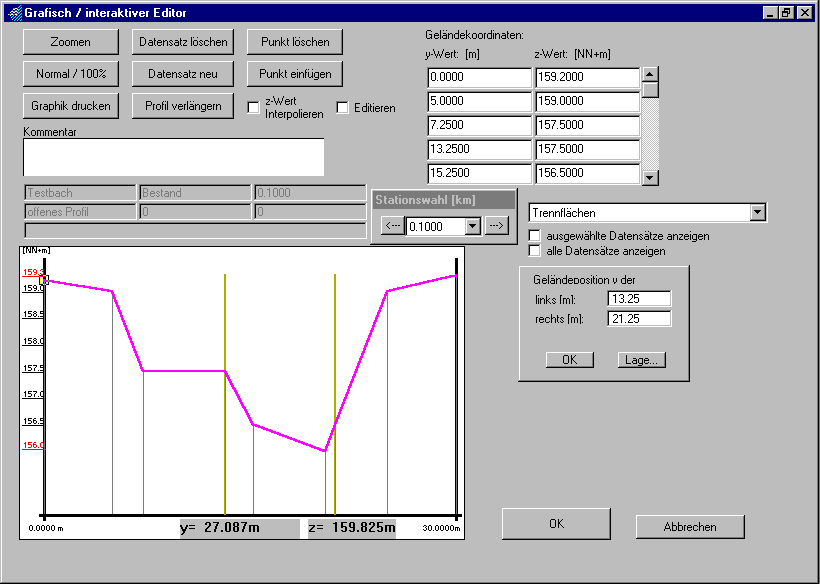
\includegraphics[width=1.0\textwidth]{PositionierungTrennflaechen}
   \caption{Positionierung der Trennfl\"{a}chen}
   \label{Einstieg Abb PositionierungTrennflaechen}
\end{figure}

Sobald Sie Werte eingegeben haben, erscheinen die Trennfl\"{a}chen in der Grafik als gelbe senkrechte Linien. Die gelben Linien k\"{o}nnen in der grafischen Darstellung bei gedr\"{u}ckter linker Maustaste an die gew\"{u}nschte Position im Querprofil verschoben werden. Parallel dazu  werden die entsprechenden aktualisierten Werte im Sonderdialog angezeigt. Wenn Sie den Sonderdialog geschlossen haben, k\"{o}nnen Sie diesen jederzeit durch Klick in der Grafik oder auf das Listenfeld wieder aktivieren. 

Wurde, wie im vorhergehenden Abschnitt beschrieben, bereits ein Datensatz Rauheiten angelegt, so bewirkt jedes Ver�ndern der Trennfl�chen eine automatische Anpassung der Rauheiten, sofern sich allen drei Fliesszonen (links Vorland, Haupt�ffnung und rechtes Vorland) ein eindeutiger Rauheitswert zuordnen l�sst. Ist letzteres nicht der Fall, d.h. wenn innerhalb einer Fliesszone verschiedene Rauheitswerte definiert sind, werden die Rauheiten beibehalten.

Die Position der Trennfl\"{a}chen sollte in jedem Fall festgelegt werden, auch wenn es sich um einen einteiligen
Querschnitt handelt (die Trennfl\"{a}chen w\"{a}ren dann nach au{\ss}en zu legen), da sich andere Programmfunktionen (z.B.
Interpolation, Rauheiten global \"{a}ndern) an den Trennfl\"{a}chen orientieren.




\subsection{Durchstr\"{o}mte Bereiche festlegen}

Neben der Lage der Trennfl\"{a}chen sind in jedem Fall auch stets die linke und rechte Grenze des abflu{\ss}wirksamen Querschnitts
einzugeben. Das hei{\ss}t Totwasserzonen bzw. nicht am Abflu{\ss}geschehen beteiligte Bereiche sind abzugrenzen. Die
Verbindungslinie der Abflu{\ss}-Grenzpunkte ist dar\"{u}ber hinaus im Lageplan einzutragen. Nur die gleichzeitige Betrachtung von
Querprofil und Lageplan kann hier zu einer nachvollziehbaren Festlegung f\"{u}hren. Eine willk\"{u}rliche Verschiebung der
Grenzpunkte allein im Querprofil ist unzul\"{a}ssig.

Die Dateneingabe erfolgt \"{a}hnlich wie bei der Festlegung der Lage der Trennfl\"{a}chen. Allerdings sind in dem hier
erscheinenden Sonderdialog links und rechts sowohl $y$- wie auch $z$-Werte einzugeben. Die Plausibilit\"{a}t wird \"{u}berpr\"{u}ft.
Die Darstellung in der Grafik erfolgt durch senkrechte blaue Linien, die am oberen Bildrand unabh\"{a}ngig von der H\"{o}he der
Werte miteinander verbunden und bei gedr\"{u}ckter linker Maustaste verschiebbar sind.
\begin{figure}[hpbt]
   \centering
   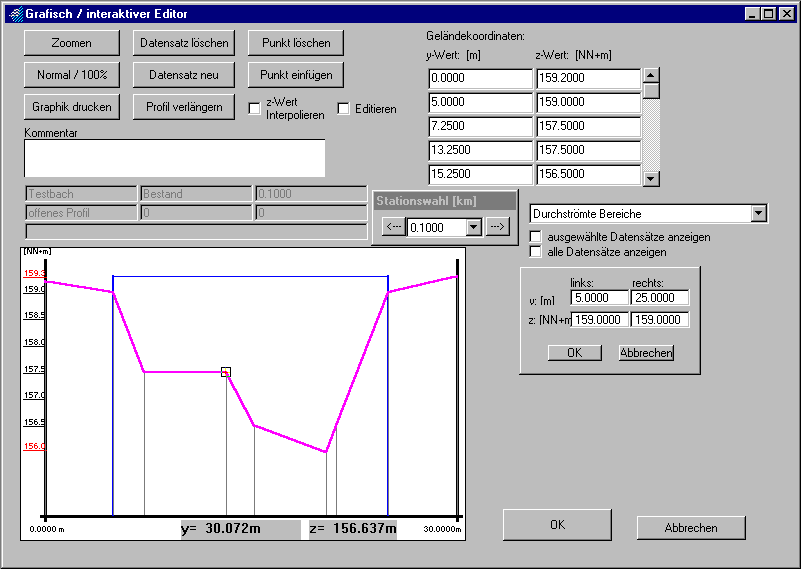
\includegraphics[width=1.0\textwidth]{DurchstroemteBereiche}
   \caption{Abgrenzung der durchstr\"{o}mten Bereiche von Totwasserzonen}
   \label{Einstieg Abb Totwasserzonen}
\end{figure}


\subsection{Georeferenzierung}

Um �berschwemmungsgebiete auszuweisen und zu visualisieren, bzw. auch um mit \wspwin{}-Mapper arbeiten zu k�nnen, m�ssen f�r jedes Profil und jeden Profilpunkt Gauss-Kr�ger-Koordinaten vorliegen. Hierzu m�ssen zun�chst die Datens�tze ''Rechtswert'' und ''Hochwert'' neu angelegt werden. In der Regel ist es ausreichend, wenn f�r den Anfangs- und Endpunkt Koordinaten eingef�gt werden. �ber das Interpolationssymbol rechts neben dem Listknopf k�nnen die fehlenden Werte automatisch zwischen geschaltet werden.
 
\begin{figure}[hpbt]
   \centering
   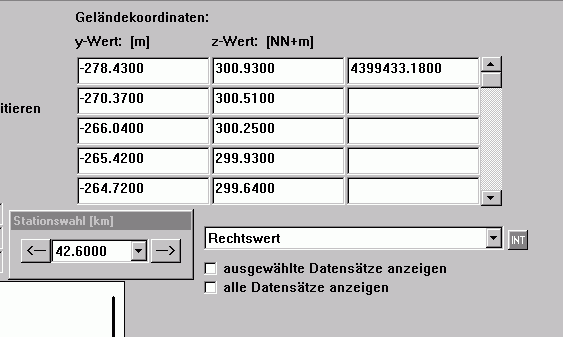
\includegraphics[width=1.0\textwidth]{gauss_krueger}
   \caption{Interpolation fehlender Gauss-Kr�ger-Koordinaten}
   \label{Einstieg Abb Interpolation}
\end{figure}


\subsection{Beispiel Profilbearbeitung}

Erzeugen sie jetzt f\"{u}r den Zustand \afz{Bestand} (siehe Abschnitt~\ref{Einstieg Subsec BeispielZustandsdatei}) drei
Profile im Abstand von jeweils $0,10\unit{km}$.

\subsubsection{Profilschl\"{u}ssel anlegen}
\"{U}ber die Schaltfl\"{a}che \schalter{Neues Profil} in der Maske \dialog{Erfassung/Editierung der Zustandsdatei} gelangen Sie in
den Profilschl\"{u}ssel-Dialog. Geben Sie hier folgendes ein:
\begin{quote}
   \begin{tabular}{ll}
      Gew\"{a}ssername:    &  \beisp{Testbach} \\
      Station:             &  \beisp{0,1} \\
      Zustand:             &  \beisp{Bestand} \\
      Verzweigungskennung: &  \beisp{0} \\
      Profilkennung:       &  \beisp{0} \\
      Profilnummer:        &  \beisp{1} \\
   \end{tabular}
\end{quote}
Mit \schalter{OK} gelangen Sie automatisch in den alphanumerischen Editor.

\subsubsection{Gel\"{a}ndeh\"{o}he eingeben}
Im alphanumerischen Editor finden Sie nun eine Tabelle, in die die folgenden Gel\"{a}ndekoordinaten eingegeben werden m\"{u}ssen.
\begin{quote}
   \begin{tabular}{ccccc}
      $y$-Wert $\mathrm{[m]}$ & $z$-Wert $\mathrm{[NN\!+\!m]}$ & \hspace{1cm} &
      $y$-Wert $\mathrm{[m]}$ & $z$-Wert $\mathrm{[NN\!+\!m]}$ \\[6pt]
      \beisp{~0,00}  & \beisp{159,20}  &  & \beisp{20,50} & \beisp{156,00} \\
      \beisp{~5,00}  & \beisp{159,00}  &  & \beisp{21,25} & \beisp{156,50} \\
      \beisp{~7,25}  & \beisp{157,50}  &  & \beisp{25,00} & \beisp{159,00} \\
      \beisp{13,25}  & \beisp{157,50}  &  & \beisp{30,00} & \beisp{159,30} \\
      \beisp{15,25}  & \beisp{156,50}
   \end{tabular}
\end{quote}

Speichern Sie nun die Eingabe indem sie mit \schalter{OK} den Editor verlassen. Sie erhalten eine Meldung, da{\ss} mindestens
Gel\"{a}ndeh\"{o}he, Trennfl\"{a}chen, durchstr\"{o}mte Bereiche und Rauheiten angegeben werden m\"{u}ssen und Sie werden gefragt, ob
\wspwin{} diese Datens\"{a}tze automatisch anlegen soll. Best\"{a}tigen Sie die automatische Generierung. Haben Sie im Vorfeld
keine Festlegung zur automatischen Generierung der Rauheiten getroffen (vgl. Abschnitt~\ref{Installation Subsec
Standardeinstellungen}), so erhalten Sie die Meldung, da{\ss} der Datensatz \afz{Rauheit} noch nicht erstellt wurde.

In der Profiltabelle erscheint nun Ihre neu angelegte Profildatei. Markieren Sie diese und wechseln Sie in den
grafisch-interaktiven Editor.

\subsubsection{Rauheiten festlegen}
Legen Sie nun f\"{u}r das Profil die Rauheiten an. Wenn Sie unter \menu{\marrow E\underline{x}tras \marrow
\underline{O}ptionen} eine automatische Generierung (Abschnitt~\ref{Installation Subsec Standardeinstellungen}) aktiviert
haben, wurde der Datensatz Rauheit (je nach Einstellung $k_S$- oder $k_{ST}$-Wert) bereits angelegt und die Werte mit null
vorbesetzt. Falls nicht, m\"{u}ssen Sie zun\"{a}chst einen neuen Datensatz erstellen. Mit \schalter{Datensatz neu} \"{o}ffnet sich
eine Auswahlliste, aus der Sie bitte \afz{Rauheit-ks} ausw\"{a}hlen.

Wurden bei der automatischen Generierung \autor{Manning-Strickler}-Rauheiten angelegt, so m\"{u}ssen Sie zun\"{a}chst diesen
Datensatz l\"{o}schen und k\"{o}nnen erst im Anschlu{\ss} daran den Datensatz \afz{Rauheit-ks} erstellen. Bei einer automatischen
Generierung des Rauheitsdatensatzes nach \autor{Darcy-Weisbach} sind diese Ma{\ss}nahmen nicht erforderlich.

In der Eingabemaske rechts oben erscheint jetzt eine zus\"{a}tzliche Spalte mit der Bezeichnung \afz{Rauheit~ks~[m]}. Geben
Sie hier die folgenden Werte ein:
\begin{quote}
   \begin{tabular}{ccccc}
      $\mathbf{y}$-\textbf{Wert} $\mathbf{\mathrm[m]}$   & $\mathbf{k_S~\mathrm{[m]}}$ & \qquad &
      $\mathbf{y}$-\textbf{Wert} $\mathbf{\mathrm[m]}$   & $\mathbf{k_S~\mathrm{[m]}}$ \\[6pt]
      \beisp{~0,00}  &  \beisp{0,20}   && \beisp{20,50} &   \beisp{0,03} \\
      \beisp{~5,00}  &  \beisp{0,20}   && \beisp{21,25} &   \beisp{0,02} \\
      \beisp{~7,25}  &  \beisp{0,05}   && \beisp{25,00} &   \beisp{0,02} \\
      \beisp{13,25}  &  \beisp{0,03}   && \beisp{30,00} &   \beisp{0,02} \\
      \beisp{15,25}  &  \beisp{0,03}
   \end{tabular}
\end{quote}
Ist die Spalte f\"{u}r die Rauheiten im Spreadsheet leer, so werden die Zwischenwerte von \wspwin{} automatisch aufgef\"{u}llt.
Sind jedoch die Rauheiten mit $0,00$ vorbelegt (z.B. durch zwischenzeitliches Speichern der Profildaten), so m\"{u}ssen Sie
auch die Zwischenwerte \"{u}berschreiben.

Markieren Sie dazu beispielsweise in der Grafik den Bereich $0,00\unit{m}$ bis $7,25\unit{m}$ mit gedr\"{u}ckter Maustaste. In
dem Dialog \dialog{Bereiche editieren} wird der markierte Bereich angezeigt. Geben Sie die Rauheit f\"{u}r diesen Bereich in
das Feld
\begin{quote}
   neuer Wert: \quad \beisp{0,2}
\end{quote}
ein und best\"{a}tigen Sie mit \schalter{OK}. In gleicher Weise verfahren Sie mit den \"{u}brigen Bereichen. Um die Werte zu
speichern, verlassen Sie den Editor mit \schalter{OK}.

\subsubsection{Definition der Trennfl\"{a}chen}
Im n\"{a}chsten Schritt erfolgt die Festlegung der Trennfl\"{a}chen. Sofern nicht automatisch generiert, legen Sie mit
\schalter{Datensatz neu} zun\"{a}chst den Datensatz \afz{Trennfl\"{a}chen} an. Der Sonderdialog \dialog{Trennfl\"{a}chen} zeigt Ihnen
nun zun\"{a}chst die Lage der Trennfl\"{a}chen am Rand Ihres Profils.

Verschieben Sie die linke Trennfl\"{a}che (gelbe Linie) mit gedr\"{u}ckter linker Maustaste an die Position $13,25\mathrm{m}$.
Verfahren Sie analog mit der rechten Trennfl\"{a}che bis zur Position $21,25\mathrm{m}$. \"{O}ffnen Sie mit \schalter{Lage...}
den Dialog zur Lagebeschreibung der Trennfl\"{a}che und \"{a}ndern sie diese auf der rechten Profilseite in \afz{B\"{o}schungsfu{\ss}}.
Best\"{a}tigen Sie die Eingabe der Lagebeschreibung und der Trennfl\"{a}chen mit \schalter{OK}.

\subsubsection{Beschr\"{a}nkung des durchstr\"{o}mten Bereichs}
Analog zur Festlegung der Trennfl\"{a}chen erfolgt die Abgrenzung der Totwasserbereiche. Legen Sie dazu ggf. den Datensatz
\afz{Durchstr\"{o}mte Bereiche} neu an. Der Sonderdialog enth\"{a}lt folgende Angaben:
\begin{quote}
   \begin{tabular}{lrr}
      links:   &  $y =\:\:0,00\unit{m}$    &  $z = 159,20\unit{NN\!+\!m}$  \\
      rechts:  &  $y = 30,00\unit{m}$      &  $z = 159,30\unit{NN\!+\!m}$
   \end{tabular}
\end{quote}
Verschieben Sie nun wieder mit der Maus die blaue Begrenzungslinie auf
\begin{quote}
   \begin{tabular}{lrr}
      links:   &  $y =\:\:5,00\unit{m}$    &  $z = 159,00\unit{NN\!+\!m}$  \\
      rechts:  &  $y = 25,00\unit{m}$      &  $z = 159,00\unit{NN\!+\!m}$
   \end{tabular}
\end{quote}
Best\"{a}tigen Sie die Eingabe mit \schalter{OK}.

\subsubsection{Profil kopieren}
Sie k\"{o}nnen nun, um weitere Profile zu erstellen, die Eingabe f\"{u}r die nachfolgenden Profile ebenfalls von Hand vornehmen.
Mit der Funktion \schalter{Profil aufnehmen} aus der Maske \dialog{Erfassung/Editierung der Zustandsdatei} kann aber auch
eine komplette Kopie des Profils erstellt werden. Sie m\"{u}ssen dann lediglich den Profilschl\"{u}ssel \"{a}ndern.

Mit dem Schalter \schalter{Profil aufnehmen} gelangen sie in einen  Dateiauswahldialog. Markieren Sie hier Ihre eben
erstellte Profildatei. Die Frage, ob das Profil kopiert werden soll, beantworten Sie mit \schalter{ja} und gelangen so in
das Dialogfenster zur Eingabe des Profilschl\"{u}ssels. \"{A}ndern sie die Werte
\begin{quote}
   \begin{tabular}{ll}
      Station:       &  \beisp{0,2} \\
      Profilnummer:  &  \beisp{2}
   \end{tabular}
\end{quote}
Das kopierte Profil erscheint in der Profiltabelle. Wiederholen Sie diesen Vorgang zur Erstellung des Querprofils~3,
mit der Station $0,3\unit{km}$.

\subsubsection{Bereiche editieren}
Die Profile~2 und 3 liegen jeweils $0,5\unit{m}$ \"{u}ber dem vorhergehenden Querschnitt. Sie k\"{o}nnen dazu die jeweiligen
Koordinaten der Gel\"{a}ndeh\"{o}he von Hand mit Hilfe der Editoren \"{a}ndern. Mit dem Dialog \dialog{Bereiche editieren} bietet
sich Ihnen jedoch noch eine andere M\"{o}glichkeit. \"{O}ffnen Sie dazu zun\"{a}chst Profil~2 im grafisch-interaktiven Editor.
W\"{a}hlen sie aus dem Auswahlfeld die Gel\"{a}ndeh\"{o}he. Es erscheint der Dialog \dialog{Bereiche editieren}. Geben Sie ein:
\begin{quote}
   Offset:  \quad \beisp{0,05}
\end{quote}
Markieren Sie die Checkbox \checkbox{alle y-Werte \"{a}ndern} und best\"{a}tigen sie mit \schalter{OK}. Alle Gel\"{a}ndeh\"{o}henpunkte
sind jetzt um $0,05\unit{m}$ erh\"{o}ht. Verfahren Sie auf gleiche Weise mit dem Querprofil~3. Die H\"{o}hendifferenz von Profil~1
zu 3 betr\"{a}gt $0,10\unit{m}$.


\clearpage
%%%%%%%%%%%%%%%%%%%%%%%%%%%%%%%%%%%%%%%%%%%%%%%%%%%%%%%%%%%%%%%%%%%%%%%%%%%%%%%%%%%%%%%%%%%%%%%%%%%%%%%%%%%%%%%%%%%%%%%%%%%%
\section{Randbedingungen}
%%%%%%%%%%%%%%%%%%%%%%%%%%%%%%%%%%%%%%%%%%%%%%%%%%%%%%%%%%%%%%%%%%%%%%%%%%%%%%%%%%%%%%%%%%%%%%%%%%%%%%%%%%%%%%%%%%%%%%%%%%%%

\subsection{Die Abflussdatei}
\label{Einstieg Subsec Abflussdatei}

F\"{u}r die hydraulische Berechnung der Wasserspiegellagen sind Randbedingungen, wie zum Beispiel der Abflu{\ss} erforderlich. Der
Abflu{\ss} kann in jedem Profil einen anderen Wert annehmen. Damit besteht die M\"{o}glichkeit, in Ann\"{a}herung an die nat\"{u}rlichen
Gegebenheiten l\"{a}ngerer Berechnungsabschnitte seitliche Zufl\"{u}sse oder Ausleitungen zu ber\"{u}cksichtigen.

Der ma{\ss}gebende Reibungsverlust zwischen den Profilen $(i-1)$ und $(i)$ wird aus dem arithmetischen Mittel der
querschnittsspezifischen mit $Q_{i-1}$ bzw. $Q_i$ gebildeten Energielinienneigungen ermittelt (vergleiche
Abschnitt~\ref{Einfuehrung Subsec TheoretischeGrundlagen}). Hieraus folgt, da{\ss} die Querprofile so zu w\"{a}hlen sind, da{\ss}
bei einer Wassermengen\"{a}nderung zwischen $(i-1)$ und $(i)$ eine Mittelung zul\"{a}ssig erscheint. Eine Verzweigungsstelle
sollte etwa in der Mitte zwischen zwei Querprofilen liegen.

Vor jeder Spiegellinienberechnung ist eine Abflu{\ss}datei zu erstellen. Eine Abflu{\ss}datei ist jeweils immer einer
Verkn\"{u}pfungsdatei (einem Zustand) zugeordnet. Wenn Sie bereits eine Zustandsdatei gew\"{a}hlt haben, bezieht sich das
Dialogfenster zur Erstellung einer Abflu{\ss}datei (Abbildung~\ref{Einstieg Abb AbflussdateiEditieren}), das unter dem
Men\"{u}punkt \menu{\marrow Z\underline{u}stand \marrow \underline{A}bflu{\ss}daten/Wasser\-spie\-gel\-fixierungen} erscheint, auf
diese Zustandsdatei. Haben Sie noch keine Verkn\"{u}pfungsdatei gew\"{a}hlt, erscheint zun\"{a}chst das Dialogfenster zur Auswahl
einer Vernetzungsdatei aus dem aktuellen Projekt. Der Men\"{u}punkt zur Eingabe der Abflu{\ss}datei ist nur aktiv, wenn vorher
alle anderen Fenster (z.B. \dialog{Grafik-Editor}, \dialog{Editieren der Zustandsdatei} usw.) geschlossen sind.
\begin{figure}[hbt]
   \centering
   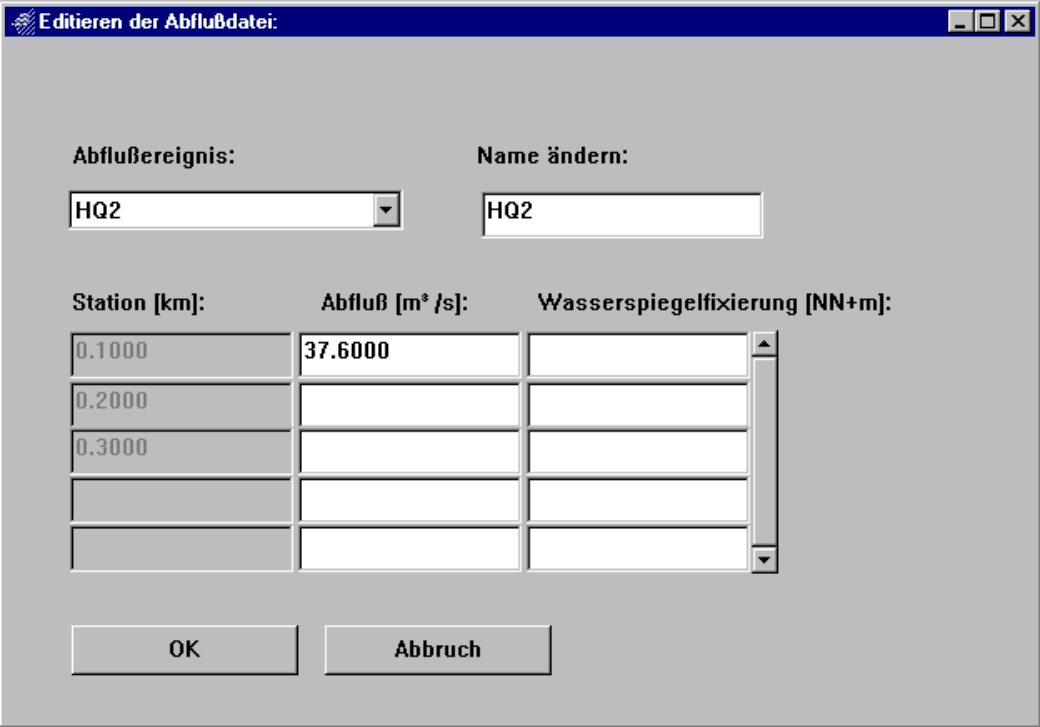
\includegraphics[width=0.7\textwidth]{AbflussdateiEditieren}
   \caption{Der Dialog zum Editieren der Abflu{\ss}datei}
   \label{Einstieg Abb AbflussdateiEditieren}
\end{figure}

Das Dialogfenster \dialog{Editieren der Abflu{\ss}datei} ist wie folgt aufgebaut: Links oben befindet sich ein Listenfeld
mit allen definierten Abflu{\ss}zust\"{a}nden. Solange Sie noch keine Abflu{\ss}datei erstellt haben, finden sich hier lediglich
die Eintr\"{a}ge \afz{neu}. Neben dem Listenfeld ist ein Editierfeld eingef\"{u}gt, in dem Sie die Bezeichnung f\"{u}r den jeweils
im Listenfeld angezeigten Abflu{\ss}zustand neu definieren k\"{o}nnen. Hier vergeben Sie also f\"{u}r den bislang unbenannten
Abflu{\ss}zustand einen neuen Namen (z.B. HQ5), indem Sie diesen \"{u}berschreiben. Der Name mu{\ss} mindestens zwei Zeichen
umfassen. In der Abflu{\ss}tabelle der unteren Bildh\"{a}lfte k\"{o}nnen Sie schlie{\ss}lich Abflu{\ss}werte f\"{u}r dieses Abflu{\ss}ereignis an
s\"{a}mtlichen Stationen, die in Ihrer Strangtabelle definiert wurden, eingeben. Es m\"{u}ssen mindestens zwei Stationen
definiert sein.

Geben Sie bitte nur an den Stationen Werte ein, an denen sich der Abflu{\ss} gegen\"{u}ber der vorherigen Station \"{a}ndert. Die
Abflu{\ss}-Felder von Stationen, an denen sich der Abflu{\ss} nicht \"{a}ndert, k\"{o}nnen leer bleiben. Allerdings mu{\ss} insgesamt an
mindestens einer (der kleinsten) Station ein Abflu{\ss} eingegeben werden.

Falls Sie mehrere Abflu{\ss}ereignisse f\"{u}r einen Zustand definieren m\"{o}chten, w\"{a}hlen Sie aus dem Listenfeld
\feld{Abflu{\ss}ereignis} \afz{neu}. Anschlie{\ss}end erhalten Sie wieder eine neue, zun\"{a}chst noch leere Tabelle, in die Sie
wiederum Abflu{\ss}werte eingeben k\"{o}nnen. Dieser Vorgang ist so oft zu wiederholen, wie Abflu{\ss}zust\"{a}nde definiert werden
sollen. S\"{a}mtliche definierten Abflu{\ss}ereignisse werden schlie{\ss}lich im Listenfeld angezeigt. Die angezeigte Tabelle bezieht
sich auf das jeweils im Listenfeld angezeigte Abflu{\ss}ereignis. Bei der Eingabe der Steuerdaten f\"{u}r die
Spiegellinienberechnung k\"{o}nnen Sie sp\"{a}ter eines dieser Ereignisse ausw\"{a}hlen.

Neben den Abfl\"{u}ssen k\"{o}nnen an den einzelnen Stationen auch Wasserspiegelfixierungen (gemessene Wasserspiegelh\"{o}hen)
eingegeben werden. Die eingegebenen Werte werden im Rahmen der Spiegellinienberechnung sp\"{a}ter sowohl in die L\"{a}ngs- wie
auch in die Querprofildatei eingetragen und k\"{o}nnen so mit den berechneten Werten verglichen werden.

\subsubsection{Beispiel}
Legen sie nun f\"{u}r die in der folgenden Tabelle angegebenen Abflu{\ss}ereignisse eine Abflu{\ss}datei an. Schlie{\ss}en Sie dazu
zun\"{a}chst alle noch ge\"{o}ffneten Dialogfenster.
\begin{quote}
   \begin{tabular}{p{4cm}p{1.5cm}p{1.5cm}p{1.5cm}p{1.5cm}p{1.5cm}}
      Abflu{\ss}ereignis:                & HQ1    & HQ2    &  HQ3   &  HQ4   &  HQ5   \\
      Abflu{\ss} in $\mathrm{[m^3/s]}$:  & $36,6$ & $37,6$ & $38,6$ & $39,6$ & $40,6$
   \end{tabular}
\end{quote}
W\"{a}hlen Sie aus dem Men\"{u} \menu{\marrow Zustand} das Untermen\"{u} \menu{\marrow Abflu{\ss}daten/Wasserspiegelfixie\-rungen}. In den
aufgerufenen Dialog geben Sie im Feld \feld{Name \"{a}ndern} die Bezeichnung f\"{u}r das Abflu{\ss}ereignis \afz{HQ1} ein. Der Wert
f\"{u}r den Abflu{\ss} an der Station $0,10\unit{km}$ betr\"{a}gt $36,6\unit{m^3/s}$.
\begin{quote}
   \begin{tabular}{ll}
      Name \"{a}ndern:                       &  \beisp{HQ1} \\
      Abflu{\ss} an Station $0,10\unit{km}$: &  36,6
   \end{tabular}
\end{quote}
\"{O}ffnen Sie, nachdem Sie den Wert eingetragen haben, das Listenfeld und w\"{a}hlen Sie \afz{neu}. Sie erhalten eine neue
Abflu{\ss}tabelle in der Sie mit der Eingabe fortfahren.

\subsection{Die Verlustdatei}
Zu den Randbedingungen einer Wasserspiegellagenberechnung geh\"{o}ren auch lokale Verluste. Diese k\"{o}nnen unter anderem durch
pl\"{o}tzliche Querschnitts\"{a}nderungen hervorgerufen werden. Diese Verluste werden in einer eigenen Verlustdatei gespeichert.
N\"{a}here Erl\"{a}uterungen zum Umgang mit Einzelverlusten enthalten die Abschnitte~\ref{Fortgeschrittene Subsec Einzelverluste}
und~\ref{Fortgeschrittene Subsec Einstellungen}.


\clearpage
%%%%%%%%%%%%%%%%%%%%%%%%%%%%%%%%%%%%%%%%%%%%%%%%%%%%%%%%%%%%%%%%%%%%%%%%%%%%%%%%%%%%%%%%%%%%%%%%%%%%%%%%%%%%%%%%%%%%%%%%%%%%
\section{Berechnen}
%%%%%%%%%%%%%%%%%%%%%%%%%%%%%%%%%%%%%%%%%%%%%%%%%%%%%%%%%%%%%%%%%%%%%%%%%%%%%%%%%%%%%%%%%%%%%%%%%%%%%%%%%%%%%%%%%%%%%%%%%%%%

\subsection{Fliessgesetze}
\label{Einstieg Subsec Fliessgesetze}

Das grundlegende Verfahren zur Berechnung des Wasserspiegels mit dem \autor{Bernoulli}'schen Energieh\"{o}henvergleich ist in
Abschnitt~\ref{Einfuehrung Subsec TheoretischeGrundlagen} beschrieben. Zur Ermittlung des Energieliniengef\"{a}lles bietet
\wspwin{} dem Anwender sieben Berechnungsmethoden, die alle auf den Flie{\ss}gesetzen von \autor{Manning-Strickler} bzw.
\autor{Prandtl-Colebrook} beruhen.

\subsubsection{Die Theorie nach Manning-Strickler}
Wird die Berechnung der Reibungsverluste nach \autor{Manning-Strickler} durchgef\"{u}hrt, so werden die folgenden
Berechnungsans\"{a}tze nach \cite{FelkelCanisius} verwendet. Ber\"{u}cksichtigt wird jeweils nur eine Rauheit f\"{u}r linkes Vorland,
Flu{\ss}bett und rechtes Vorland. Sind mehr als drei Rauheiten im Profil angegeben, so erfolgen Mittelungen f�r die Werte in den jeweiligen Teilabflu{\ss}querschnitten.
\begin{equation}
   v = k_{ST} \cdot r_{hy}^{2/3} \cdot I_E^{1/2}
\end{equation}
Hydraulische Radien $r_{hy,j}$:
\begin{equation}
   \label{Einstieg Gl HydraulRadius}
   r_{hy,L} = A_L / U_L  \qquad  r_{hy,F} = A_F / U_F  \qquad  r_{hy,R} = A_R / U_R
\end{equation}
Die spezifischen Geschwindigkeiten $w_j$ in $\mathrm{[m/s]}$ betragen:
\begin{equation}
   \label{Einstieg Gl SpezifGeschwindigkeit}
   \begin{split}
      w_L &= k_{ST} \cdot r_{hy}^{2/3} \cdot (l_F/l_L)^{1/2} \\
      w_F &= k_{ST} \cdot r_{hy}^{2/3} \\
      w_R &= k_{ST} \cdot r_{hy}^{2/3} \cdot (l_F/l_R)^{1/2}
   \end{split}
\end{equation}
Hydraulische Leitwerte $C_j$ in $\mathrm{[m^3/s]}$:
\begin{equation}
   C_L = A_L \cdot w_L  \qquad  C_F = A_F \cdot w_F  \qquad  C_R = A_R \cdot w_R
\end{equation}
Gesamtabflu{\ss} $Q$ in $\mathrm{[m^3/s]}$:
\begin{equation}
   Q = \sum C_j \cdot I_E^{1/2}
      \label{Einstieg Gl Gesamtabfluss}
\end{equation}
Teilgeschwindigkeiten $v_j$ in $\mathrm{[m/s]}$:
\begin{equation}
   v_L = w_L \cdot I_E^{1/2}  \qquad  v_F = w_F \cdot I_E^{1/2}  \qquad  v_R = w_R \cdot I_E^{1/2}
\end{equation}
Teilabfl\"{u}sse $Q_j$ in $\mathrm{[m^3/s]}$:
\begin{equation}
   Q_L = v_L \cdot A_L  \qquad  Q_F = v_F \cdot A_F  \qquad  Q_R = v_R \cdot A_R
\end{equation}
Geschwindigkeitsverteilungsbeiwert  $\alpha$ (\autor{Coriolis}-Beiwert):
\begin{equation}
   \label{Einstieg Gl Geschwindigkeitsverteilung}
   \alpha = \frac{1}{A_{ges}} \cdot \sum \left( \frac{v_j^3 \cdot A_j}{v_m^3} \right)
\end{equation}
Impulsstromverteilungsbeiwert $\alpha'$ (\autor{Boussinesq}-Beiwert):
\begin{equation}
   \label{Einstieg Gl Impulsstromverteilung}
   \alpha' = \frac{1}{A_{ges}} \cdot \sum \left( \frac{v_j^2 \cdot A_j}{v_m^2} \right)
\end{equation}
Geschwindigkeitsh\"{o}he $h_k$ in $\mathrm{[m]}$:
\begin{equation}   h_k = \alpha \cdot \frac{v_m^2}{2g}
\end{equation}
\autor{Froud}'sche Zahl $Fr$:
\begin{equation}
   \label{Einstieg Gl Froudezahl}
   Fr = \frac{\sqrt{\alpha} \cdot v_{ges}}{\sqrt{g \cdot A_{ges}/b_{ges}}}
\end{equation}


\subsubsection{Die Theorie nach Prandtl-Colebrook}
Im Falle der Anwendung des allgemeinen Flie{\ss}gesetzes nach
\autor{Prandtl-Colebrook} \cite{DVWK1991} gilt f\"{u}r den vollkommen rauhen Bereich:
\begin{equation}
   v = \sqrt{\frac{8g \cdot r_{hy} \cdot I_E}{\lambda}}
\end{equation}
mit
\begin{equation}
   \frac{1}{\lambda} = 2\lg \left( \frac{14,84 \cdot r_{hy}}{k_S} \right)
      \label{Einstieg Gl LambdaBeiwert}
\end{equation}
ach entsprechender Umformung der Gleichung f\"{u}r den Reibungswert ergeben sich folgende Berechnungsans\"{a}tze f\"{u}r die
Hilfsgr\"{o}{\ss}en wobei die Rauheiten $k_{S,j}$  in $\mathrm{m}$ einzusetzen sind:
\begin{equation}
  \begin{split}
      w_L &= 2\sqrt{8g} \cdot \lg(14,84 \cdot r_{hy,L}/k_{S,L}) \cdot (r_{hy,L} \cdot l_F/l_L)^{1/2} \\
      w_F &= 2\sqrt{8g} \cdot \lg(14,84 \cdot r_{hy,F}/k_{S,F}) \cdot r_{hy,L}^{1/2} \\
      w_R &= 2\sqrt{8g} \cdot \lg(14,84 \cdot r_{hy,R}/k_{S,R}) \cdot (r_{hy,R} \cdot l_F/l_R)^{1/2}
   \end{split}
\end{equation}
Wie schon bei dem Flie{\ss}gesetz nach \autor{Manning-Strickler} rechnet auch der Ansatz nach \autor{Prandtl-Colebrook} mit
nur drei Rauheiten. Alle \"{u}brigen Berechnungsans\"{a}tze zur Bestimmung der hydraulischen Kennwerte eines Profils sind
dieselben wie vorher. F\"{u}r den Abflu{\ss} im geschlossenen Profil (Durchla{\ss}) wird das vollst\"{a}ndige Widerstandsgesetz von
\autor{Prandtl-Colebrook} \cite{PressSchroeder}, das auch im \"{U}bergangsbereich gilt, angewendet. Die L\"{o}sung des
impliziten Widerstandsgesetzes erfolgt durch \autor{Newton}-Iteration.

\subsubsection{Theorie nach Einstein (Manning-Strickler)}
Die Berechnung basiert auf dem Flie{\ss}gesetz von \autor{Manning-Strickler}. Nach \autor{Einstein} kann bei Anwendung dieses
Flie{\ss}gesetzes eine durchschnittliche Rauheit im Profil ohne Iteration berechnet werden.
\begin{equation}
   k_{ST,ges} = \left( \frac{U_{ges}}{\sum \left(U_i/k_{ST,i}^{3/2} \right)}\right)^{2/3}
\end{equation}
Dieser Ansatz f\"{u}r geometrisch einheitliche Profile wird hier sinngem\"{a}{\ss} auf die Teilabflu{\ss}querschnitte des gegliederten
Querschnitts \"{u}bertragen, d.h. die Durchschnittsrauheiten werden getrennt f\"{u}r Vorl\"{a}nder und Flu{\ss}bett berechnet.

\subsubsection{Theorie nach Prandtl-Colebrook + Bewuchs nach Kaiser}
Basierend auf dem Flie{\ss}gesetz von \autor{Prandtl-Colebrook} hat \autor{Kaiser} eine Theorie entwickelt, die mit Hilfe der
spezifischen Vegetationsanstr\"{o}mfl\"{a}che $\omega_P \mathrm{[m]}$  Bewuchs be\-r\"{u}ck\-sich\-tigt (siehe
Abschnitt~\ref{Sonderprofile Subsec Kaiser}). Unabh\"{a}ngig davon k\"{o}nnen mehrere Einzelrauheiten $k_S \mathrm{[m]}$ pro
Teilabflu{\ss}querschnitt angegeben werden.

Die Berechnung der Durchschnittsrauheiten bzw. mittleren Rauheitsbeiwerten gestaltet sich bei der Anwendung der
Flie{\ss}gesetze nach \autor{Prandtl-Colebrook} etwas aufwendiger. Da die Widerstandsbeiwerte $\lambda_i$ von den
hydraulischen Radien abh\"{a}ngen, die zugeordneten Teilfl\"{a}chen jedoch nicht bekannt sind, ist nur eine iterative Berechnung
des Gesamtwiderstandsbeiwertes m\"{o}glich. Der mittlere Rauheitsbeiwert kann nach~\cite{SchroederW} wie folgt ermittelt
werden:
\begin{equation}
   \lambda_{ges} = \frac{ \sum \left(U_i \cdot \lambda_i \right)}{U_{ges}}
      \label{Einstieg Gl LambdaKaiser}
\end{equation}
In einem ersten Schritt werden die Widerstandsbeiwerte $\lambda_i$ mit dem hydraulischen Radius des gesamten
Profilabschnittes bestimmt. So lassen sich nach Gleichung~\ref{Einstieg Gl LambdaKaiser} die hydraulischen Teilradien
berechnen. Werden diese in Gleichung~\ref{Einstieg Gl LambdaBeiwert} eingesetzt, ergeben sich die einzelnen
Widerstandsbeiwerte $\lambda_i$. Die Berechnung wird dann abgebrochen, wenn sich der Gesamtwiderstandsbeiwert nach
Gleichung~\ref{Einstieg Gl LambdaKaiser} nicht mehr \"{a}ndert.


\subsubsection{Theorie nach Prandtl-Colebrook + Bewuchs nach Nuding}
Die Theorie nach \autor{Nuding} ber\"{u}cksichtigt ebenfalls den Bewuchs. Hierf\"{u}r m\"{u}ssen die Bewuchsdurchmesser $D_P$ sowie
die Bewuchsabst\"{a}nde $a_x$ in und $a_y$ quer zur Flie{\ss}richtung angegeben werden (siehe Abschnitt~\ref{Sonderprofile Subsec
Nuding}). Unterschiedliche Einzelrauheiten werden ber\"{u}cksichtigt.

\subsubsection{Theorie nach Prandtl-Colebrook + Bewuchs nach Mertens}
Neben unterschiedlichen Einzelrauheiten werden auch Bewuchsabst\"{a}nde und Bewuchsdurchmesser ber\"{u}cksichtigt (siehe
Abschnitt~\ref{Sonderprofile Subsec Mertens}).

\subsubsection{Theorie nach Prandtl-Colebrook + Bewuchs nach Pasche}
Wie schon bei der Theorie nach \autor{Mertens} werden unterschiedlichen Einzelrauheiten, Bewuchsabst\"{a}nde und
Bewuchsdurchmesser ber\"{u}cksichtigt (siehe Abschnitt~\ref{Sonderprofile Subsec Pasche}).


\subsection{Eingabe der Steuerdaten}

Um die Steuerdaten f\"{u}r die Spiegellinienberechnung anzugeben, w\"{a}hlen Sie aus dem Men\"{u} \menu{\marrow \underline{B}erechnung
\marrow \underline{S}piegellinienberechnung}. Beachten Sie, da{\ss} zuvor eine Zustandsdatei ausgew\"{a}hlt sein mu{\ss}. Sofern sie
nicht schon einmal Daten f\"{u}r die Berechnung angegeben haben, erscheint die Meldung, da{\ss} noch keine Steuerdaten vorhanden
sind.
\begin{figure}[hbt]
   \centering
   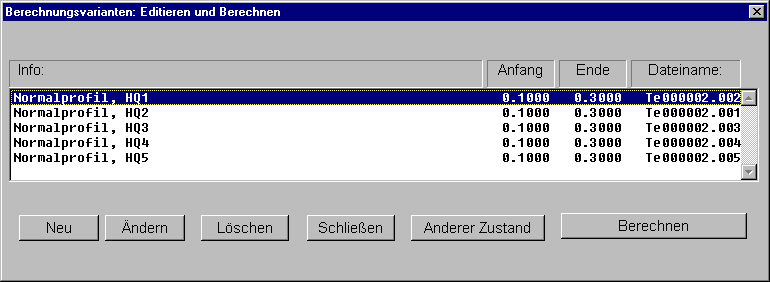
\includegraphics[width=1.0\textwidth]{AuswahlBerechnungsvarianten}
   \caption{Dialogmaske zur Auswahl und zum \"{A}ndern der Berechnungsvarianten}
   \label{Einstieg Subsec AuswahlBerechnungsvarianten}
\end{figure}

Mit Hilfe der Schaltfl\"{a}che \schalter{Neu} gelangen Sie in die Maske \dialog{Steuerdaten}. Hier finden Sie vier
Registerkarten in denen Sie Einstellungen zur Art und Weise der Berechnung, zu Randbedingungen und zur Ausgabeform treffen
k\"{o}nnen. \"{U}ber die Schaltfl\"{a}che \schalter{andere Wahl} k\"{o}nnen sie die Zustandsdatei wechseln, f\"{u}r die die Steuerdaten
vereinbart werden sollen.

Wurde bereits im Vorfeld eine Berechnung durchgef\"{u}hrt, gelangen sie in das Dialogfenster \dialog{Berechnungsvarianten:
Editieren und Berechnen} (Abbildung~\ref{Einstieg Subsec AuswahlBerechnungsvarianten}). Hier haben sie die M\"{o}glichkeit
vorhandene Berechnungsvarianten auszuw\"{a}hlen, zu \"{a}ndern oder neue Berechnungsvarianten zu erstellen. Die Zustandsdatei kann
hier \"{u}ber die Schaltfl\"{a}che \schalter{anderer Zustand} gewechselt werden.

F\"{u}r eine Berechnungsvariante m\"{u}ssen zun\"{a}chst die Basisdaten vereinbart werden. Ganz oben auf der entsprechenden
Registerkarte (Abbildung~\ref{Einstieg Subsubsec Basisdaten}) erscheint ein Feld in dem Sie einen Text mit bis zu
60~Zeichen zu Ihrer Berechnungsvariante eingeben k\"{o}nnen. Darunter l\"{a}{\ss}t sich der Berechnungsabschnitt einschr\"{a}nken. Die
Listenfelder enthalten alle von Ihnen bei der Profileingabe angegebenen Stationen. Voreingestellt sind zun\"{a}chst das
Anfangs- und Endprofil Ihrer bei der Profileingabe festgelegten Kilometrierung. Beachten Sie bei der Eingabe bitte, da{\ss}
das Anfangsprofil stets flu{\ss}ab liegt.

Liegt bezogen auf den Anfangswasserspiegel schie{\ss}ender Abflu{\ss} vor, so mu{\ss} dies \"{u}ber die Checkbox \checkbox{schie{\ss}ender
Abflu{\ss}} angegeben werden. Die Berechnung beginnt dann am OW-Profil.

Um eine Wasserspiegellagenberechnung durchf\"{u}hren zu k\"{o}nnen, mu{\ss} der Wasserspiegel im Anfangsprofil entweder zahlenm\"{a}{\ss}ig
bekannt sein, oder sich aus einer vorgegebenen hydraulischen Randbedingung berechnen lassen. Das Anfangsprofil ist je nach
Flie{\ss}zustand das unterste Profil f\"{u}r den str\"{o}menden bzw. das oberste f\"{u}r den schie{\ss}enden Abflu{\ss}. F\"{u}r die Anfangsbedingung
kann demnach gew\"{a}hlt werden:
\begin{description}
   \item [Bekannte Wasserstand-Abflu{\ss}-Beziehung:]
      Die Wasserspiegellage kann direkt in das Feld \feld{Anfangswasserspiegel} eingegeben werden. Dies trifft kann
      beispielsweise auf bewegliche Wehre mit einem fest vorgegebenen Stauziel zu. In diesem Fall legen Sie das
      Anfangsprofil direkt oberhalb des Wehres. Der Anfangswasserstand entspricht dann dem Stauziel.
   \item [Querschnitt oberhalb eines Flie{\ss}wechsels:]
      An einem Flie{\ss}wechsel tritt zwangsl\"{a}ufig die Grenztiefe (\"{U}bergang Str\"{o}men - Schie{\ss}en) auf. Diese kann mit Hilfe des
      Extremalprinzips im Anfangsprofil des Berechnungsabschnitts iterativ berechnet werden. Markieren Sie dazu
      \checkbox{Grenztiefe}.
   \item[Querschnitt mit ann\"{a}hernd gleichf\"{o}rmigem Abflu{\ss}:]
      Aktivieren Sie den Punkt \checkbox{sta\-tio\-n\"{a}r gleichf\"{o}rmig}, wird die Normalwassertiefe iterativ aus dem
      angegebenen Energieliniengef\"{a}l\-le (absolut) im ersten Profil berechnet.
   \item[Querschnitt oberhalb eines festen Wehres mit vollkommenem \"{U}berfall:]
      Der An\-fangs\-wasserstand wird hier mit Hilfe der \autor{Poleni}-Formel aus der Kronenh\"{o}he des Wehres und der
      \"{U}berfallh\"{o}he berechnet. Markieren Sie die Checkbox \checkbox{Wehr am Anfang}.
\end{description}

F\"{u}r den Fall, da{\ss} keine der beschriebenen hydraulischen Randbedingungen zutreffen, ist die Berechnungsstrecke flu{\ss}abw\"{a}rts
zu verl\"{a}ngern. Man sch\"{a}tzt einen Anfangswasserstand und f\"{u}hrt eine Wasserspiegellagenberechnung durch. Der bei der
Sch\"{a}tzung gemachte Fehler wirkt sich nach oberstrom von Profil zu Profil (abh\"{a}ngig von Gef\"{a}lle und Flie{\ss}geschwindigkeit)
immer weniger aus, so das bei entsprechender Verl\"{a}ngerung der vorangestellten Berechnungsstrecke der Einflu{\ss} auf den
Anfangswasserstand des eigentlich betrachteten Flu{\ss}abschnitts vernachl\"{a}ssigbar gering ist.
\begin{figure}[bth]
   \centering
   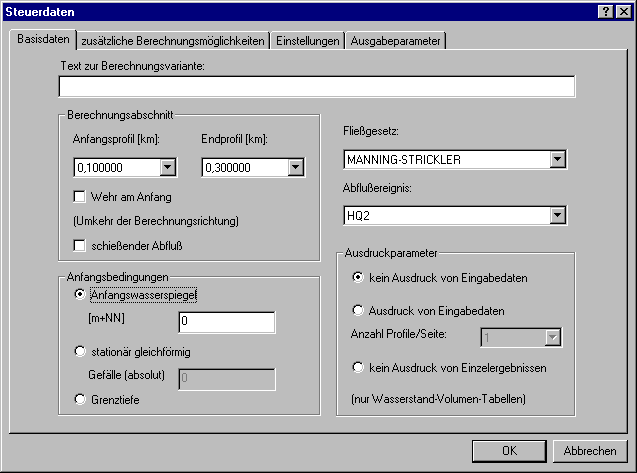
\includegraphics[width=1.0\textwidth]{Basisdaten}
   \caption{Dialog zum Festlegen der Basisdaten f\"{u}r die Spiegellinienberechnung}
   \label{Einstieg Subsubsec Basisdaten}
\end{figure}

Voraussetzung f\"{u}r diese Vorgehensweise ist jedoch, da{\ss} der neue Ausgangswasserstand nicht im Staubereich einer noch weiter
unterhalb gelegenen St\"{o}rung liegt. Zur Probe f\"{u}r die richtige \"{U}berl\"{a}nge wird die Berechnung mit einem anderen
Anfangswasserstand wiederholt, wobei sich angen\"{a}hert derselbe Wert f\"{u}r den Wasserspiegel des eigentlichen Anfangsprofils
ergeben mu{\ss}.

Auf der rechten Seite der Registerkarte \dialog{Basisdaten} finden sie ein Listenfeld zur Auswahl der in
Abschnitt~\ref{Einstieg Subsec Fliessgesetze} n\"{a}her beschriebenen Flie{\ss}gesetze. Darunter k\"{o}nnen sie ein Abflu{\ss}ereignis
aus Ihrer Abflu{\ss}datei (Abschnitt~\ref{Einstieg Subsec Abflussdatei}) ausw\"{a}hlen, f\"{u}r das die Berechnung durchgef\"{u}hrt
werden soll. Beachten Sie bei der Auswahl des Flie{\ss}gesetzes, da{\ss} im Vorfeld die f\"{u}r die Berechnung zugeh\"{o}rigen
Rauheiten nach Abschnitt~\ref{Einstieg Subsec Rauheit} definiert sind. Es kann z.B. keine Berechnung nach der
Flie{\ss}theorie von \autor{Manning-Strickler} auf Grundlage der \autor{Darcy-Weisbach}'schen Rauheiten erfolgen.

Bez\"{u}glich der Darstellung der Ergebnistabelle k\"{o}nnen hier weiterhin folgende Einstellungen getroffen werden:
\begin{description}
   \item [Kein Ausdruck von Eingabedaten:]
      Es werden nur die Berechnungsergebnisse ausgegeben.
   \item [Ausdruck von Eingabedaten:]
      Dem Ergebnisausdruck werden die Eingabedaten vorangestellt. Die Anzahl der Profile pro Seite kann zus\"{a}tzlich
      festgelegt werden.
   \item [Kein Ausdruck von Einzelergebnissen:]
      Sofern Sie neben der normalen Berechnung die Ausgabe der Abflu{\ss}-Wasserstand-Volumen-Tabellen gew\"{a}hlt haben, haben
      Sie hier die M\"{o}glichkeit nur die Ergebnisse der Tabellen ohne die normale Wasserspiegellagenberechnung auszugeben.
\end{description}

Die Funktionen auf den Registerkarten \dialog{zus\"{a}tzliche Berechnungsm\"{o}glichkeiten}, \dialog{Einstellungen} und
\dialog{Ausgabeparameter} werden im Kapitel~\ref{Fortgeschrittene} erl\"{a}utert.


\subsubsection{Beispiel Steuerdaten}

Legen Sie im folgenden f\"{u}r den \afz{Testbach} eine Berechnungsvariante an. Schlie{\ss}en Sie dazu zun\"{a}chst alle noch
ge\"{o}ffneten Dialogfenster. W\"{a}hlen Sie aus dem Men\"{u} \menu{\marrow \underline{B}erechnen \marrow
\underline{S}piegellinienberechnung}.

Da im Vorfeld noch keine Steuerdaten vereinbart wurden, f\"{u}hrt man sie zun\"{a}chst in den Dialog zur Erstellung einer neuen
Berechnungsvariante. In die Registerkarte \dialog{Basisdaten} tragen Sie bitte ein:
\begin{quote}
   \begin{tabular}{ll}
      Text zur Berechnungsvariante:       &  \beisp{Normalprofil, HQ1} \\
      Anfangsprofil:                      &  \beisp{0,1} \\
      Endprofil:                          &  \beisp{0,3} \\
      Flie{\ss}gesetz:                        &  \beisp{Prandtl-Colebrook} \\
      Abflu{\ss}ereignis:                     &  \beisp{HQ1} \\
      Anfangswasserspiegel:               &  \beisp{158,0} \\
   \end{tabular}
\end{quote}
F\"{u}r die Ausdrucksparameter geben Sie \afz{kein Ausdruck von Eingabedaten} an. Speichern Sie die Eingaben mit
\schalter{OK}.


\subsection{Die Berechnung starten}

Nachdem Sie die Dialogmaske zum Editieren der Steuerdaten mit \schalter{OK} verlassen und damit alle Eingabedaten
gespeichert haben, gelangen Sie automatisch in ein Fenster, in dem s\"{a}mtliche bereits angelegten Berechnungsvarianten
mit ihrer Kennzeichnung, dem Anfangs- und Endprofil des Berechnungsabschnitts und dem Dateinamen aufgelistet sind
(Abbildung~\ref{Einstieg Subsec AuswahlBerechnungsvarianten}). Diese \"{U}bersicht wird an sp\"{a}teren Stellen (z.B. Auswahl
des L\"{a}ngsschnitts zum Plotten) noch mehrfach erscheinen. Aus dieser \"{U}bersichtsmaske heraus k\"{o}nnen sie bereits angelegte
Berechnungsvarianten jederzeit wieder \"{a}ndern, bearbeiten, l\"{o}schen oder neue Varianten anlegen.

Diese Berechnungsvariantenverkn\"{u}pfungsdatei ist stets einer Zustandsdatei zugeordnet. \"{U}ber die Schaltfl\"{a}che
\schalter{Anderer Zustand} k\"{o}nnen Sie auch Varianten aus anderen Zust\"{a}nden bearbeiten. \"{U}ber \schalter{Schlie{\ss}en}
verlassen Sie die Maske.

Den eigentlichen Berechnungsvorgang starten Sie \"{u}ber den Schalter \schalter{Berechnen}. Sie k\"{o}nnen eine oder mehrere
Varianten zur Berechnung markieren (STRG + Mausklick bzw. STRG + Pfeiltaste) und ausw\"{a}hlen.

Beim Berechnungsvorgang wird ein externes Programm gestartet. Nach Abschlu{\ss} der Berechnung erhalten Sie eine R\"{u}ckmeldung.
Der Benutzer kann nach erfolgreicher Berechnung die Ergebnisdateien im Unterverzeichnis
\datei{\textbackslash dath} einsehen.

Im Rahmen der Berechnung werden in den L\"{a}ngs- und Querprofilen automatisch alte berechnete Wasserspiegellagen gel\"{o}scht und
die aktuellen Werte eingetragen. Bei Markierung und Berechnung mehrerer Varianten werden auch mehrere Wasserspiegel
grafisch dargestellt.


\subsubsection{Beispiel Berechnung starten}

Legen Sie zun\"{a}chst vier weitere Berechnungsvarianten f\"{u}r die Abflu{\ss}ereignisse HQ2, HQ3, HQ4 und HQ5 an. Markieren Sie
diese im Anschlu{\ss}, indem sie die STRG-Taste gedr\"{u}ckt halten und die Varianten anklicken. Starten Sie die Berechnung
\"{u}ber den Schalter \schalter{Berechnen}.


\clearpage
%%%%%%%%%%%%%%%%%%%%%%%%%%%%%%%%%%%%%%%%%%%%%%%%%%%%%%%%%%%%%%%%%%%%%%%%%%%%%%%%%%%%%%%%%%%%%%%%%%%%%%%%%%%%%%%%%%%%%%%%%%%%
\section{Berechnungsergebnisse einsehen}
%%%%%%%%%%%%%%%%%%%%%%%%%%%%%%%%%%%%%%%%%%%%%%%%%%%%%%%%%%%%%%%%%%%%%%%%%%%%%%%%%%%%%%%%%%%%%%%%%%%%%%%%%%%%%%%%%%%%%%%%%%%%

\subsection{Der WspWin-Editor}

Der Untermen\"{u}punkt \menu{\marrow Tabelle} des Men\"{u}s \menu{\marrow Ergebnisse} erm\"{o}glicht es Ihnen, jederzeit die
tabellarischen Ergebnisse der Spiegellinienberechnung (aber auch Auswertungsergebnisse, Fehlermeldungen und beliebige
Textdateien im ASCII-Format (s.u.)) einzusehen, zu formatieren und zu drucken.

Nachdem Sie den Men\"{u}punkt gew\"{a}hlt haben, erscheint zun\"{a}chst die Maske zur Auswahl der Berechnungsvariante. Es wird ein
neues Programm, n\"{a}mlich der \wspwin{}-Editor gestartet und Ihr Berechnungsergebnis angezeigt. Der Editor ist den \"{u}blichen
Win\-dows-Konventionen entsprechend aufgebaut (vgl. z.B. Wordpad.exe).
\begin{hinweis}
   Wenn Sie im Men\"{u} \menu{\marrow E\underline{x}tras \marrow \underline{O}ptionen} in der Registerkarte
   \dialog{Verzeichnisse} den Pfad der \datei{Editor.exe} angeben, k\"{o}nnen Sie den \wspwin{}Editor auch direkt \"{u}ber das
   Men\"{u} \menu{\marrow \underline{E}rgebnisse \marrow \underline{E}ditor} starten. Sie finden die Datei im
   \wspwin{}-Installationsverzeichnis. In gleicher Weise kann aber auch ein weiterer Editor integriert werden.
\end{hinweis}

M\"{o}chten Sie eine andere Ergebnis- oder Protokolldatei im Editor einsehen (\menu{\marrow \underline{D}atei \marrow
\underline{\"{O}}ffnen...}), erscheint die in Abbildung~\ref{Einstieg Abb EditorDateiOeffnen} dargestellte Maske, die zun\"{a}chst
s\"{a}mtliche Gew\"{a}sser des aktuellen Projektes auflistet. Durch Klicken auf das +-K\"{a}stchen werden s\"{a}mtliche Zust\"{a}nde
dargestellt, die ihrerseits wieder aufgeklappt werden k\"{o}nnen, um zu entscheiden, ob Berechnungsergebnisse oder Ergebnisse
der Auswerteprogramme dargestellt werden sollen. Hat man sich f\"{u}r eine der beiden Varianten entschieden, werden rechter
Hand s\"{a}mtliche vorhandenen Berechnungsvarianten aufgelistet und man kann durch Markierung und Best\"{a}tigung mit
\schalter{OK} eine Variante einsehen. Zus\"{a}tzlich zu den Berechnungsergebnissen werden auch die Fehlerdateien aufgelistet.
Sie k\"{o}nnen ebenfalls mit Hilfe des Editors eingesehen werden.
\begin{figure}[htp]
   \centering
   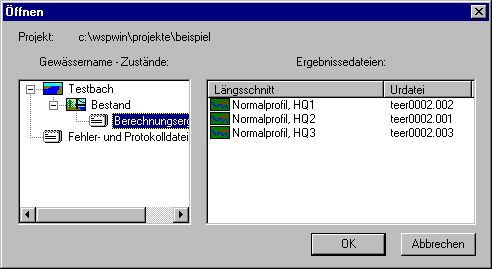
\includegraphics[width=0.8\textwidth]{EditorDateiOeffnen}
   \caption{Datei im Editor \"{o}ffnen}
   \label{Einstieg Abb EditorDateiOeffnen}
\end{figure}

Will man davon abweichend eine beliebige Textdatei \"{u}ber den Standard-Windows-Dialog zur Dateiauswahl \"{o}ffnen, hat man unter
dem Men\"{u}punkt \menu{\marrow \datei{D}atei} zun\"{a}chst das Untermen\"{u} \menu{\marrow Projekt s\underline{c}hlie{\ss}en} zu w\"{a}hlen.
Danach kann man \"{u}ber \menu{\marrow Datei \underline{\"{o}}ffnen} eine beliebige Textdatei \"{o}ffnen und editieren. Ebenso ist es
m\"{o}glich ein anderes Projekt mit Hilfe der Men\"{u}option \menu{\marrow \"{O}ffnen \underline{P}rojekt} auszuw\"{a}hlen.

Der Texteditor stellt bei Ergebnisdateien im ANSI-Format Seitenumbr\"{u}che durch K\"{a}stchen dar. \"{U}ber den Men\"{u}punkt
\menu{\marrow For\-ma\underline{t} \marrow Seitenwechsel} kann an der Stelle, an der sich der Cursor momentan befindet,
ein weiterer Seitenwechsel eingef\"{u}gt werden. Zum L\"{o}schen des Seitenumbruchs entfernen Sie das K\"{a}stchen wieder.
\begin{figure}
   \centering
   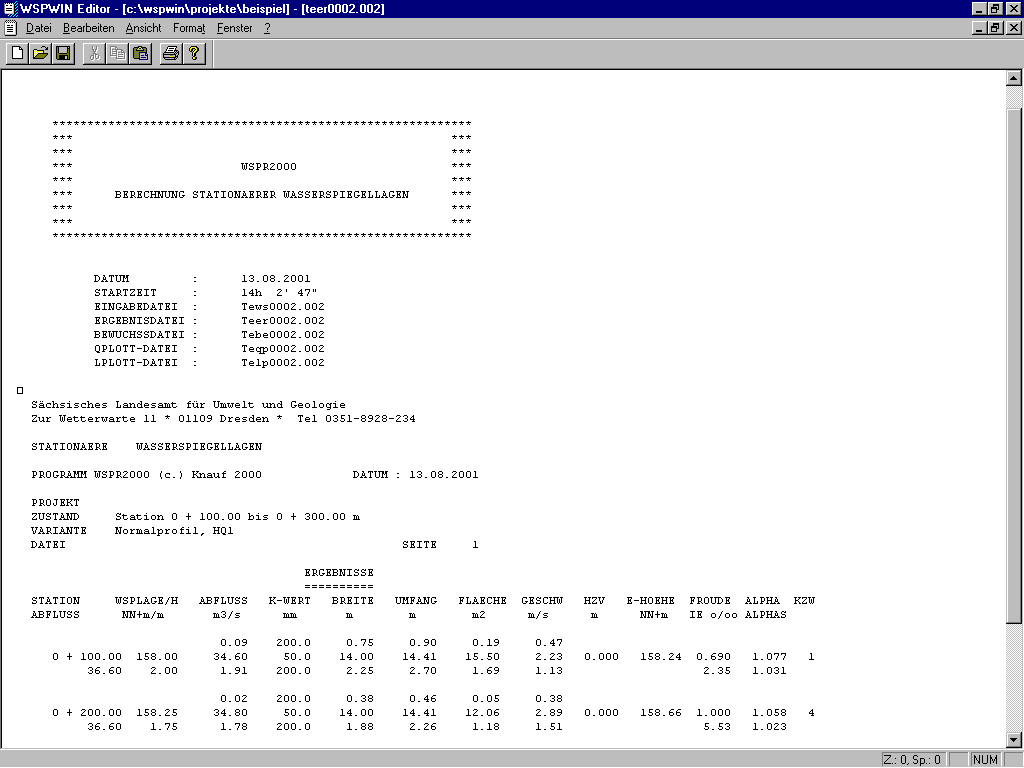
\includegraphics[width=1.0\textwidth]{Editor}
   \caption{Einsehen einer Datei im Texteditor}
   \label{Einstieg Abb Editor}
\end{figure}

Das Men\"{u} \menu{\marrow Forma\underline{t}} bietet weiterhin die M\"{o}glichkeit die Einstellungen f\"{u}r die Schriftart und das
Absatzlayout zu ver\"{a}ndern. Mit Hilfe der Funktion \menu{\marrow OEM$\leftrightarrow$ANSI} kann das Aussehen der Umlaute
und Sonderzeichen, falls erforderlich, ver\"{a}ndert werden.

Die Ergebnisse Ihrer Berechnung k\"{o}nnen auch aus dem Editor heraus gedruckt werden. Nachdem Sie die Men\"{u}folge \menu{\marrow
\underline{D}atei \marrow \underline{D}rucken...} gew\"{a}hlt haben, erscheint der Ihnen aus anderen Windows-Anwendungen
bekannte Dialog in dem Sie Seitenformat, Druckertreiber etc. ausw\"{a}hlen k\"{o}nnen. Standardm\"{a}{\ss}ig werden Ihnen die Optionen der
Systemdruckereinstellung angezeigt. Mit \schalter{OK} starten sie den Druckvorgang, \"{u}ber \schalter{Eigenschaften} nehmen
Sie ggf. weiter Druckereinstellungen vor.


\subsubsection{Beispiel - Einsehen der Berechnungsergebnisse}

Sehen Sie die Berechnungsergebnisse Ihrer ersten Berechnungsvariante ein. W\"{a}hlen Sie dazu aus dem Men\"{u} \menu{\marrow
\underline{E}rgebnisse} den Punkt \menu{\marrow \underline{T}abelle}. Es erscheint die Dialogmaske zur Auswahl einer
Berechnungsvariante. Markieren Sie die Variante \afz{Normalprofil, HQ1} und best\"{a}tigen Sie mit \schalter{OK}.

\begin{hinweis}
   Der \wspwin{}-Editor stellt ein eigenst\"{a}ndiges Programm dar, das auch ohne das Berechnungsprogramm genutzt werden kann.
   Wenn Sie auf Ihrem Desktop eine Verkn\"{u}pfung zu der Datei \datei{Editor.exe} im Installationsverzeichnis vom \wspwin{}
   erstellen, k\"{o}nnen Sie das Programm aus Windows heraus direkt starten. Es ist so m\"{o}glich Dateien und Berechnungsergebnisse
   einzusehen, ohne da{\ss} dazu \wspwin{} aufgerufen werden mu{\ss}.
\end{hinweis}


\subsection{Erl\"{a}uterung der Abk\"{u}rzungen im Ergebnisausdruck}
\label{Einstieg Subsec Ergebnisausdruck}

Der Ergebnisausdruck in der Standardeinstellung zeigt zun\"{a}chst in der ersten Spalte der Tabelle die Stationierung des
Profils. Darunter wird der Gesamtabflu{\ss} in $\unit{[m^3/s]}$ ausgegeben. Die zweite Spalte enth\"{a}lt in der ersten Zeile die
Wasserspiegellage $W$ in $\unit{[NN\!+\!m]}$ bzw. $\unit{[HN\!+\!m]}$. Darunter steht die Wassertiefe in $\unit{[m]}$.

Die darauffolgenden Spalten gliedern sich jeweils in drei Zeilen (vgl. Abbildung~\ref{Einstieg Abb Editor}). In der
ersten Zeile stehen die Werte f\"{u}r das linke Vorland, in der dritten die des rechten Teilabflu{\ss}querschnitts. Die
mittlere Zeile gibt die Werte f\"{u}r den Flu{\ss}schlauch an.
\begin{quote}
   \begin{tabular}{p{0.15\linewidth}p{0.8\linewidth}}
      ABFLUSS \newline  m3\slash s
            &  Teilabflu{\ss} $Q_L$, $Q_F$, $Q_R$ in $\unit{[m^3/s]}$ im Flu{\ss}bett und Vorland, \\[18pt]
      K-WERT \newline m\^{}.33/s
            &  Rauheit $k_{ST,j}~\unit{[m^{1/3}/s]}$ nach \autor{Manning-Strickler} im Teilabflu{\ss}querschnitt oder \\[6pt]
      K-WERT \newline m
            &  Rauheit $k_{S,j} \unit{[m]}$ nach \autor{Darcy-Weisbach} im Teilabflu{\ss}querschnitt \\[6pt]
      BREITE \newline m
            &  Breite des Wasserspiegels in den Vorl\"{a}ndern und im Flu{\ss}schlauch \\[6pt]
      UMFANG \newline m
            &  Benetzer Umfang $U_L$, $U_F$, $U_R$ des jeweiligen Teilabflu{\ss}querschnitts in $\unit{[m]}$, \\[6pt]
      FL\"{A}CHE \newline m2
            &  Flie{\ss}querschnitte $A_L$, $A_F$, $A_R$ der jeweiligen Teilabflu{\ss}querschnitte in $\unit{[m^2]}$, \\[6pt]
      GESCHW \newline m\slash s
            &  Mittlere Flie{\ss}geschwindigkeiten $v_L$, $v_F$, $v_R$ im jeweiligen Teilabflu{\ss}querschnitt in $\unit{[m/s]}$
   \end{tabular}
\end{quote}
Im Anschlu{\ss} an die getrennte Darstellung der Flie{\ss}parameter f\"{u}r Vorl\"{a}nder und Hauptgerinne werden noch verschiedene
Kenngr\"{o}{\ss}en die den gesamten Flie{\ss}querschnitt betreffen ausgegeben.
\begin{quote}
   \begin{tabular}{p{0.15\linewidth}p{0.8\linewidth}}
      HZV \newline m
            &  Errechnete Verlusth\"{o}he $H_{ZV}~\unit{[m]}$ aus den Einzelverlusten an der Station. \\[6pt]
      E-HOEHE \newline NN + m
            &  Die berechnete H\"{o}he $H_E$ der Energielinie in $\unit{[NN\!+\!m]}$ bzw. $\unit{[HN\!+\!m]}$ f\"{u}r den
               Profilquerschnitt wird wiedergegeben \\[6pt]
      FROUDE \newline IE o\slash oo
            &  Die erste Zeile gibt die \autor{Froude}-Zahl zur Kennzeichnung des Flie{\ss}zustandes wieder (s.u.).
               Darunter wird das querschnittsspezifische Energieliniengef\"{a}lle unter Einschlu{\ss} der
               Geschwindigkeitsverteilung (Gleichung~\ref{Einstieg Gl Gesamtabfluss}) ausgegeben. \\[6pt]
      ALPHA \newline ALPHAS
            &  Geschwindigkeitsverteilungsbeiwert $\alpha$ und Impulsstromverteilungsbeiwert $\alpha'$.
   \end{tabular}
\end{quote}

Zur schnellen Orientierung und zur Kontrolle der Berechnungsart wird am rechten Rand der Ergebnislisten f\"{u}r jedes
berechnete Querprofil ein Kennungsparameter $KZW$ ausgegeben, der angibt, mit welchem Unterprogramm gerechnet wurde. In
Normalprofilen kann $KZW$ folgende Werte erhalten.
\begin{quote}
   \begin{tabular}{lp{0.8\linewidth}}
      $KZW =  0$  &  Spiegelh\"{o}he aus Spiegellinieniteration \\
      $KZW =  1$  &  Wasserstand vorgegeben \\
      $KZW =  2$  &  $k$-Wert Berechnung Flu{\ss}bett \\
      $KZW =  3$  &  $k$-Wert Berechnung Vorl\"{a}nder \\
      $KZW =  4$  &  Spiegellage ist gleich der Grenztiefe \\
      $KZW =  5$  &  Spiegellage ist gleich der Normalwassertiefe \\
      $KZW =  6$  &  Wasserstand oberhalb eines vollkommenen \"{U}berfalls \\
      $KZW =  7$  &  Spiegellage aus vorhergehendem Berechnungsabschnitt \\
      $KZW =  8$  &  Pfeilerstau nach \autor{Rehbock} \\
      $KZW =  9$  &  Wasserstand ergibt sich aus erforderlicher Mindestenergie\-h\"{o}he im Durchla{\ss}
   \end{tabular}
\end{quote}
Bei Aufstau in geschlossenen Profilen ohne \"{U}berflutung werden die Kennziffern~10 bis 19 f\"{u}r die Berechnung nach der
Flie{\ss}theorie von \autor{Manning-Strickler} und die Kennziffern~20 bis 29 f\"{u}r die Berechnung nach \autor{Prandtl-Colebrook}
vergeben.
\begin{quote}
   \begin{tabular}{lcc}
      Durchla{\ss}typ                            &  \autor{Strickler} &  \autor{Prandtl-Colebrook} \\[6pt]
      Kreisprofil                            &  $KZW = 10$        &  $KZW = 20$ \\
      Durchla{\ss} mit horizontaler Decke        &  $KZW = 11$        &  $KZW = 21$ \\
      Halbkreis oder Kreissegment            &  $KZW = 12$        &  $KZW = 22$ \\
      Maulprofil DIN~4263                    &  $KZW = 13$        &  $KZW = 23$ \\
      Maulprofil ARMCO Fibel~71              &  $KZW = 14$        &  $KZW = 24$ \\
      Wertetabelle f\"{u}r lineare Interpolation &  $KZW = 15$        &  $KZW = 25$ \\
      Eiprofil DIN~4263                      &  $KZW = 16$        &  $KZW = 26$ \\
      Maulprofil ARMCO Fibel~84              &  $KZW = 17$        &  $KZW = 27$ \\
      Ellipsenprofil ARMCO Fibel~84          &  $KZW = 18$        &  $KZW = 28$ \\
      Super-Span ARMCO Fibel~84              &  $KZW = 19$        &  $KZW = 29$
   \end{tabular}
\end{quote}
Tritt dagegen ein Aufstau mit \"{U}berflutung auf, so nimmt der $KZW$-Wert in Abh\"{a}ngigkeit vom Flie{\ss}gesetz Werte zwischen
30 und 49 an.
\begin{quote}
   \begin{tabular}{lcc}
      Durchla{\ss}typ                            &  \autor{Strickler} &  \autor{Prandtl-Colebrook} \\[6pt]
      Kreisprofil                            &  $KZW = 30$        &  $KZW = 40$ \\
      Durchla{\ss} mit horizontaler Decke        &  $KZW = 31$        &  $KZW = 41$ \\
      Halbkreis oder Kreissegment            &  $KZW = 32$        &  $KZW = 42$ \\
      Maulprofil DIN~4263                    &  $KZW = 33$        &  $KZW = 43$ \\
      Maulprofil ARMCO Fibel~71              &  $KZW = 34$        &  $KZW = 44$ \\
      Wertetabelle f\"{u}r lineare Interpolation &  $KZW = 35$        &  $KZW = 45$ \\
      Eiprofil DIN~4263                      &  $KZW = 36$        &  $KZW = 46$ \\
      Maulprofil ARMCO Fibel~84              &  $KZW = 37$        &  $KZW = 47$ \\
      Ellipsenprofil ARMCO Fibel~84          &  $KZW = 38$        &  $KZW = 48$ \\
      Super-Span ARMCO Fibel~84              &  $KZW = 39$        &  $KZW = 49$
   \end{tabular}
\end{quote}
Die folgenden Kennziffern geben Auskunft \"{u}ber weitere spezielle Berechnungsvarianten
\begin{quote}
   \begin{tabular}{lp{0.8\linewidth}}
   		$KZW =  55$  &  Normalwassertiefe f�r alle Profile \\
      $KZW =  61$  &  \"{U}berfallbeiwert wurde nach \autor{Kandaswany\slash Rouse} berechnet \\
      $KZW =  65$  &  Fl\"{a}chenberechnung nach \autor{Gauss} (Manning-Strickler) \\
      $KZW =  66$  &  Fl\"{a}chenberechnung nach \autor{Gauss} (Prandtl-Colebrook) \\
      $KZW =  70$  &  Streichwehr \\
      $KZW =  71$  &  breitkroniges Wehr \\
      $KZW =  72$  &  dachf\"{o}rmiges Wehr \\
      $KZW =  73$  &  rundkroniges Wehr \\
      $KZW =  74$  &  scharfkantiges Wehr \\
      $KZW =  77$  &  Wehr mit unterschiedlichen Kronenh\"{o}hen
   \end{tabular}
\end{quote}
Bei Teilstrecken von Verzweigungen steht vor der $KZW$-Kennziffer die jeweilige Teilstreckennummer.
\begin{quote}
   $KZW = \mathit{IVZ}*100 + KZW$
\end{quote}
Entspricht die Berechnungsrichtung der Flie{\ss}richtung (schie{\ss}ender Abflu{\ss}), so werden negative Kennziffern vergeben.
\begin{quote}
   \begin{tabular}{lp{0.8\linewidth}}
      $KZW = -1$  &  Wasserstand vorgegeben f\"{u}r schie{\ss}enden Abflu{\ss}, Anfangswasserstand im oberwasserseitigen
                     Anfangsprofil \\
      $KZW = -4$  &  Anfangswasserstand ist gleich der Grenztiefe (schie{\ss}ender Abflu{\ss}) \\
      $KZW = -5$  &  Anfangswasserstand ist gleich der Normalwassertiefe
   \end{tabular}
\end{quote}
Hinter Zahlenwerten k\"{o}nnen zus\"{a}tzliche Kennzeichen auftreten, wie z.B:
\begin{quote}
   \begin{tabular}{ll}
      *  (hinter Fl\"{a}chenwert) &  Inselbildung, Gel\"{a}nde teilweise \"{u}ber WSP \\
      DH (neben WSP-Lage)     &  Druckh\"{o}he, kein freier Wasserspiegel \\
      UE (neben WSP-Lage)     &  Durchla{\ss} wird \"{u}berstr\"{o}mt \\
      ***                     &  Energieh\"{o}he steigt nicht an
   \end{tabular}
\end{quote}
Die \autor{Froude}'sche Zahl gibt den Flie{\ss}zustand im Gerinne wieder. Es bedeuten:
\begin{quote}
   \begin{tabular}{ll}
      $Fr > 1$ &  Schie{\ss}ender Abflu{\ss} \\
      $Fr = 1$ &  Kritischer Abflu{\ss} (Flie{\ss}wechsel) \\
      $Fr < 1$ &  Str\"{o}mender Abflu{\ss} \\
      $Fr = 0$ &  Str\"{o}mung ohne freien Wasserspiegel (Druckabflu{\ss})
   \end{tabular}
\end{quote}

Die Durchstr�mungsart wird durch die Kennziffer KZD gekennzeichnet.

\begin{tabular}{ll}
	\\
	\underline{- mit Einstau der Br�ckenunterkante DKUK, keine �berstr�mung} \\
	Standardberechnung mit Verlustbeiwerte  & 0 \\
	Sch�tzstr�mung nach \autor{Schmidt}			& 1 \\
	Sch�tzstr�mung nach \autor{Knapp}				& 2 \\
	eintauchende Br�ckenplatten nach Naudascher-Medlarz	& 3 \\
	\\
	\underline{- mit �berstr�mung der Br�ckenoberkante DKOK} \\
	Standardberechnung mit Verlustbeiwerte		& 5 \\
	Sch�tzstr�mung nach \autor{Schmidt}	 			&	6 \\
	Sch�tzstr�mung nach \autor{Knapp}					&	7 \\
\end{tabular}

\subsection{Der L\"{a}ngsschnitteditor}
\label{Einstieg Subsec Laengsschnitteditor}

Nachdem Sie eine Spiegellinienberechnung erfolgreich durchgef\"{u}hrt haben, haben Sie unter dem Men\"{u}punkt \menu{\marrow
\underline{E}rgebnisse \marrow \underline{L}\"{a}ngsschnitt einsehen} die M\"{o}glichkeit, das Ergebnis der Berechnung in einer
Grafik einzusehen.
\begin{figure}[hbt]
   \centering
   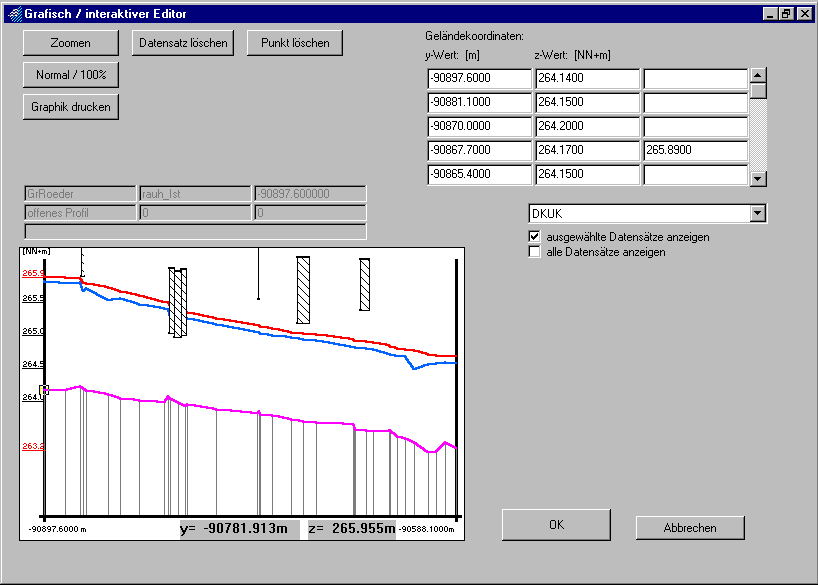
\includegraphics[width=1.0\textwidth]{Laengsschnitteditor}
      \caption{L\"{a}ngsschnitteditor}
      \label{Einstieg Abb Laengsschnitteditor}
\end{figure}

Wenn die Option gew\"{a}hlt wird erscheint, falls noch keine Vernetzungsdatei gew\"{a}hlt wurde, zun\"{a}chst wiederum die
Dialogmaske zur \dialog{Auswahl einer Zustandsdatei}. Anschlie{\ss}end werden Sie zur Auswahl einer Berechnungsvariante
aufgefordert.

W\"{a}hrend der Berechnung wird automatisch eine L\"{a}ngsschnittdatei im BCE-Format erzeugt, die im Grafik-Editor f\"{u}r
L\"{a}ngsschnitte eingesehen und sp\"{a}ter auch geplottet werden kann. Der L\"{a}ngsschnitteditor ist analog zum Grafik-Editor f\"{u}r
Querprofile aufgebaut. Der einzige Unterschied besteht darin, da{\ss} keine neuen Datens\"{a}tze angelegt werden k\"{o}nnen.
Folgende Datens\"{a}tze werden bei L\"{a}ngsschnitten automatisch erzeugt:
\begin{quote}
   \begin{labeling}[~]{Schleppspannung {[N/m2]}}
      \item[Sohlh\"{o}he]                  Lage der Sohle, grafische und alphanumerische Darstellung (magenta Linie)
      \item[B\"{o}schung li.]              Linke B\"{o}schungsoberkante, grafische und alphanumerische Darstellung (gelbe Linie)
      \item[B\"{o}schung re.]              Rechte B\"{o}schungsoberkante, grafische und alphanumerische Darstellung (orange Linie)
      \item[Ausuferung li.]            grafische und alphanumerische Darstellung (hellgr\"{u}ne Linie)
      \item[Ausuferung re.]            grafische und alphanumerische Darstellung (graue Linie)
      \item[Wasserspiegel]             Lage des Wasserspiegels, grafische und alphanumerische Darstellung (blaue Linie)
      \item[Abflu{\ss}]                    Abflu{\ss}, alphanumerisch
      \item[Schleppspannung {[N/m2]}]  Sohlschubspannung, alphanumerisch
      \item[WSP-Breite]                Wasserspiegelbreite, alphanumerisch
      \item[Energieh\"{o}he {[NN+m]}]      Energieh\"{o}he, grafische und alphanumerische Darstellung (rote Linie)
      \item[DKUK]                      Deckenunterkante (nur bei Sonderprofilen), grafische und alphanumerische
                                       Darstellung (schwarz schraffierter Kasten)
      \item[DKOK]                      Deckenoberkante (nur bei Sonderprofilen), grafische und alphanumerische Darstellung
                                       (schwarz schraffierter Kasten)
      \item[Profilart]                 Nummern analog $KZW$ (Abschnitt~\ref{Einstieg Subsec Ergebnisausdruck}, alphanumerisch
      \item[Profilkennung]             Profilkennung, alphanumerisch, 1=LL, 2=FF, 3=RR
      \item[Verzweigung]               Verzweigungskennung, alphanumerisch
      \item[Wasserspiegelfixierung]    grafische und alphanumerische Darstellung (nur wenn in Steuerdaten aktiviert und
                                       unter \menu{\marrow Zustand\marrow Abflu{\ss}daten/Wasserspiegelfixierungen} eingegeben)
      \item[Wasserspiegeldifferenz]    Differenz zwischen gemessenem und berechneten Wasserspiegel.
   \end{labeling}
\end{quote}

Die Datens\"{a}tze \afz{Sohlh\"{o}he}, \afz{B\"{o}schung li.}, \afz{B\"{o}schung re.}, die errechnete Wasserspiegelh\"{o}he sowie bei
entsprechenden Profilen ggf. die H\"{o}he der Deckenoberkante und -unterkante werden grafisch dargestellt. Sofern Sie die
Datens\"{a}tze nicht nur einzeln darstellen m\"{o}chten, haben Sie \"{u}ber das K\"{a}stchen \checkbox{alle Datens\"{a}tze anzeigen} die
M\"{o}glichkeit, sich alle angelegten Datens\"{a}tze parallel anzeigen zu lassen. Sollen nur bestimmte Datens\"{a}tze in der Grafik
angezeigt werden, so ist dies \"{u}ber die Checkbox \checkbox{ausgew\"{a}hlte Datens\"{a}tze anzeigen} m\"{o}glich.  W\"{a}hlen Sie hierzu,
jeden der darzustellenden Parameter explizit nacheinander aus dem Listenfeld mit allen Datens\"{a}tzen an. Diese werden dann
nacheinander in die Grafik \"{u}bernommen.

Die Datens\"{a}tze \afz{Wasserspiegelbreite} und \afz{Abflu{\ss}} werden Ihnen alphanumerisch in der dritten Spalte des
Spreadsheets angezeigt. Anhand der Nummer der Profilart in der dritten Spalte des Spreadsheets k\"{o}nnen Sie erkennen, ob es
sich um ein Normal- oder Sonderprofil handelt. Die Nummern entsprechen den $KZW$-Parametern im Ergebnisausdruck (siehe
Abschnitt~\ref{Einstieg Subsec Ergebnisausdruck}). Wenn Sie im Spreadsheet mit dem Cursor durch die Stationen wandern,
zeigt Ihnen ein K\"{a}stchen in der Grafik die entsprechende Position an. Automatisch erscheinen die Schl\"{u}sseldaten des
jeweiligen Profiles in der linken oberen Ecke des Fensters.

Sofern Sie das Ergebnis in Form des L\"{a}ngsschnitts nicht nur am Bildschirm einsehen, sondern auch auf Papier festhalten
m\"{o}chten, k\"{o}nnen Sie die Grafik, wie auf dem Bildschirm dargestellt, \"{u}ber die Schaltfl\"{a}che \schalter{Grafik drucken} direkt
aus dem Grafik-Editor heraus drucken. Es folgt der Standard-Windows-Dialog zur Druckereinrichtung. Bitte beachten Sie, da{\ss}
keine ma{\ss}st\"{a}bliche Darstellung mit vielen Details erstellt wird. Dies wiederum ist \"{u}ber die Eingabe von Plotoptionen f\"{u}r
die Erstellung des eigentlichen Ergebnisl\"{a}ngsschnitts m\"{o}glich. \"{U}ber die Option \schalter{Grafik drucken}, die im \"{u}brigen
auch bei Querprofilen verf\"{u}gbar ist, kann man sich aber zur schnellen \"{U}bersicht einen einfach zu erstellenden
Ergebnisausdruck anfertigen.


\subsubsection{Beispiel}
Nachdem Sie den Editor zur Einsicht der tabellarischen Ergebnisse \"{u}ber \menu{\marrow Datei~\underline{b}eenden} wieder
verlassen haben, k\"{o}nnen Sie die Berechnungsergebnisse des Beispiels auch anschaulich im L\"{a}ngsschnitt einsehen und
ausdrucken. W\"{a}hlen sie dazu aus dem Men\"{u} \menu{\marrow \underline{E}r\-geb\-nisse \marrow \underline{L}\"{a}ngsschnitt
einsehen} aus. Setzen Sie einen Haken vor das K\"{a}stchen \checkbox{alle Datens\"{a}tze anzeigen}. Die Grafik wird nun mit allen
berechneten Datens\"{a}tzen dargestellt. Um die Darstellung zu drucken verwenden Sie die Schaltfl\"{a}che \schalter{Grafik
drucken} und folgen den Anweisungen des Windows-Dialogs zur Druckereinstellung.


%%%%%%%%%%%%%%%%%%%%%%%%%%%%%%%%%%%%%%%%%%%%%%%%%%%%%%%%%%%%%%%%%%%%%%%%%%%%%%%%%%%%%%%%%%%%%%%%%%%%%%%%%%%%%%%%%%%%%%%%%%%%
\section{Programm beenden}
%%%%%%%%%%%%%%%%%%%%%%%%%%%%%%%%%%%%%%%%%%%%%%%%%%%%%%%%%%%%%%%%%%%%%%%%%%%%%%%%%%%%%%%%%%%%%%%%%%%%%%%%%%%%%%%%%%%%%%%%%%%%

\"{U}ber den Men\"{u}punkt \menu{\marrow \underline{P}rojekt \marrow \underline{B}eenden} beenden Sie Ihre Arbeit mit \wspwin{}.
            %  Kapitel  4
   \graphicspath{{Fortgeschrittene/eps/}} \cleardoublepage
%%%%%%%%%%%%%%%%%%%%%%%%%%%%%%%%%%%%%%%%%%%%%%%%%%%%%%%%%%%%%%%%%%%%%%%%%%%%%%%%%%%%%%%%%%%%%%%%%%%%%%%%%%%%%%%%%%%%%%%%%%%%

\chapter{Fortgeschrittene Handhabung}
\label{Fortgeschrittene}

%%%%%%%%%%%%%%%%%%%%%%%%%%%%%%%%%%%%%%%%%%%%%%%%%%%%%%%%%%%%%%%%%%%%%%%%%%%%%%%%%%%%%%%%%%%%%%%%%%%%%%%%%%%%%%%%%%%%%%%%%%%%

%%%%%%%%%%%%%%%%%%%%%%%%%%%%%%%%%%%%%%%%%%%%%%%%%%%%%%%%%%%%%%%%%%%%%%%%%%%%%%%%%%%%%%%%%%%%%%%%%%%%%%%%%%%%%%%%%%%%%%%%%%%%
\section{Projekte organisieren}
%%%%%%%%%%%%%%%%%%%%%%%%%%%%%%%%%%%%%%%%%%%%%%%%%%%%%%%%%%%%%%%%%%%%%%%%%%%%%%%%%%%%%%%%%%%%%%%%%%%%%%%%%%%%%%%%%%%%%%%%%%%%

\subsection{Die Projekt\"{u}bersicht}

In der Projekt\"{u}bersicht werden alle in der Projektauswahlmaske aufgelisteten Projekte mit ihren Zust\"{a}n\-den und den
zugeh\"{o}rigen Daten aufgelistet. Sie k\"{o}nnen so den Aufbau Ihres Projektes und seine Organisation jederzeit nachvollziehen.
\begin{figure}[hbt]
   \centering
   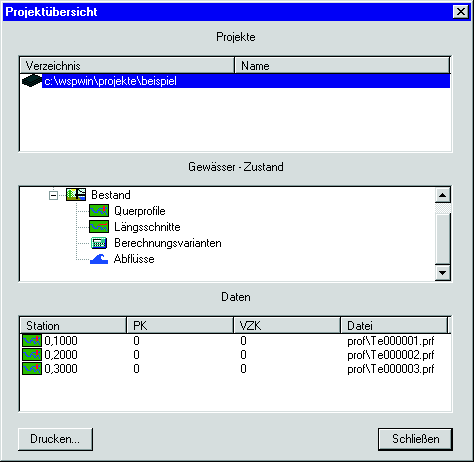
\includegraphics[width=0.8\textwidth]{Projektuebersicht}
   \caption{Dialogfenster \dialog{Projekt\"{u}bersicht}}
   \label{Fortgeschrittene Abb Projektuebersicht}
\end{figure}

In dem mittleren Fenster werden die einzelnen Komponenten des ausgew\"{a}hlten Projektes dargestellt. Ausgehend von
Gew\"{a}ssernamen sind dies zun\"{a}chst die einzelnen Zu\-st\"{a}n\-de des Gew\"{a}ssers. Innerhalb der Zust\"{a}nde sind die zugeh\"{o}rigen
Querprofile, L\"{a}ngsschnitte, Berechnungsvarianten und Abfl\"{u}sse aufgelistet. Das untere Fenster zeigt die vorhandenen Daten
(Profildateien, L\"{a}ngsschnittdateien, Berechnungsvariantendateien und Abflu{\ss}dateien).


\subsection{Projekte kopieren}

\"{U}ber die Men\"{u}folge \menu{\marrow \underline{P}rojekt \marrow Projekt \underline{s}peichern unter} haben Sie die
M\"{o}glichkeit, da{\ss} gerade ge\"{o}ffnete Projekt in ein anderes Verzeichnis zu kopieren, um dort z.B. zu Testzwecken
Einstellungen zu modifizieren. Es erscheint ein Dialog, der Sie zur Eingabe des neuen Projektverzeichnisses auffordert.
Wenn das angegebene Verzeichnis noch nicht existiert, wird es automatisch neu angelegt. \"{U}ber den Schalter
\schalter{Suchen...} haben Sie aus der Standard-Windows-Maske heraus auch die M\"{o}glichkeit, einen Pfad zu suchen, der dann
im Editierfeld \feld{Verzeichnis} angezeigt wird und hier oder in dem Dialog \dialog{Projekt speichern unter} erg\"{a}nzt
werden kann.


\subsection{Projekte archivieren}

Projekte, die momentan nicht mehr gebraucht werden, k\"{o}nnen \"{u}ber \wspwin{} archiviert werden. W\"{a}hlen Sie hierzu die
Men\"{u}folge \menu{\marrow \underline{P}rojekt \marrow \underline{A}rchivieren \marrow archivieren} und selektieren Sie
anschlie{\ss}end das zu archivierende Projekt. Sie werden aufgefordert, da{\ss} Verzeichnis einzugeben, in dem Sie Ihr Projekt
archivieren m\"{o}chten. Sie k\"{o}nnen in diesem Arbeitsschritt einen neuen Namen f\"{u}r Ihr Verzeichnis vergeben und auch mehrere
Unterverzeichnisse anlegen. Das entsprechende Projekt wird anschlie{\ss}end aus der Projekt\"{u}bersichtsliste entfernt.

Mittels \menu{\marrow \underline{P}rojekt \marrow \underline{A}rchivieren \marrow zur\"{u}ckladen} kann es jederzeit wieder
aufgenommen werden. Eine Liste der archivierten Projekte befindet sich in der Datei \datei{wspwin.arh}, die sich im
Verzeichnis der Datei \datei{wspwin.prj} befindet und nicht ver\"{a}ndert werden sollte. Die Projektarchivierung beinhaltet
keine Datenkomprimierung.


\subsection{Projekte importieren}

\"{U}ber den Men\"{u}punkt \menu{\marrow \underline{P}rojekt \marrow \underline{I}mportieren \marrow Projekt
auf\underline{n}ehmen} k\"{o}nnen Projekte, die nicht im Projektvereichnis aufgelistet sind, importiert werden. Dies macht
beispielsweise Sinn, wenn sie Projektdaten von anderen Anwendern geschickt bekommen und weiterverarbeiten m\"{o}chten. Im
gleichen Men\"{u}punkt finden Sie auch das Untermen\"{u} \menu{ \marrow Projekteintrag \underline{l}\"{o}schen}. Im Gegensatz zu der
Funktion \schalter{L\"{o}schen} aus der Projektauswahlmaske heraus wird hier nur der Projekteintrag entfernt, das Verzeichnis
mit seinen Daten bleibt bestehen.


\subsection{Fremddaten}

\subsubsection{HYDRA-WSP}
\wspwin{} erm\"{o}glicht Ihnen die Konvertierung von bereits existierenden \"{a}lteren Datens\"{a}t\-zen im Format von HYDRAWSP
(LWA-Format) in ein Format, das von \wspwin{} sowohl rechnerisch wie auch grafisch verarbeitet werden kann.

Nach Aufruf des Men\"{u}punktes \menu{ \marrow \underline{P}rojekt \marrow \underline{F}remddaten  \marrow
\underline{H}YDRAWSP} erscheint ein Dialogfenster, das Sie zur Auswahl einer oder mehrerer zu konvertierender Dateien
auffordert.  Die Dateien m\"{u}ssen \"{u}ber die Endung \datei{*.wsp} verf\"{u}gen (ggf. umbenennen). Die konvertierten Dateien werden
alle in ihrem aktuellen Projekt abgelegt, das Ihnen in einer Sicherheitsabfrage nochmals angezeigt wird.

F\"{u}r jede konvertierte Datei wird eine neue Vernetzungsdatei eingerichtet. Dazu sind jeweils die Schl\"{u}sseldaten
Gew\"{a}ssername, Datum und Zustand von Ihnen zu definieren. Hierbei erscheint zun\"{a}chst noch einmal der Name der zu
konvertierenden Datei, den Sie mit \schalter{OK} best\"{a}tigen, gefolgt von dem bekannten Dialogfenster zur Definition der
Schl\"{u}sseldaten. Dieser Vorgang wird so oft wiederholt, wie Sie zu konvertierende Dateien ausgew\"{a}hlt haben. Nach der
letzten Datei wird schlie{\ss}lich ein Konvertierungsprogramm gestartet, das die neuen Vernetzungs- und Profildateien f\"{u}r Sie
anlegt. Die Dateien k\"{o}nnen dann wie gewohnt von Ihnen weiter bearbeitet werden. Auch die Steuerdaten f\"{u}r die Berechnung
werden \"{u}bernommen. Beachten Sie aber, da{\ss} jeweils nur der erste Abflu{\ss}zustand in das \wspwin{}-Format \"{u}berf\"{u}hrt wird.

Nach Abschlu{\ss} der Konvertierung wird eine Meldung ausgegeben. Meldungen \"{u}ber aufgetretene Fehler k\"{o}nnen in der Datei
\datei{\mbox{error.log}} eingesehen werden. Ein Protokoll der Umwandlung findet sich in der Datei \datei{lwa2b.log}.

\subsubsection{DA66}
\wspwin{} kann mit einem Zusatzmodul zur Konvertierung von Vermessungsdaten im Format DA66 ins \wspwin{}-Format geliefert
werden. Die Option ist dann unter dem Men\"{u}punkt \menu{ \marrow \underline{P}rojekt  \marrow \underline{F}remddaten \marrow
\underline{D}A66} verf\"{u}gbar. Nach diesem Aufruf werden Sie in einem Standard-Windows-Dialog zur Auswahl der DA66-Datei
aufgefordert. Sobald Sie die Datei ausgew\"{a}hlt haben, m\"{u}ssen Sie die Schl\"{u}sseldaten f\"{u}r eine neue Vernetzungsdatei angeben.
Im Anschlu{\ss} daran wird die Datei konvertiert.

\begin{figure}[hbt]
   \centering
   \input{Fortgeschrittene/tab/FormatDA66.tab}
   \caption{Ausschnitt aus einer Datei im DA66-Format}
   \label{Fortgeschrittene Abb FormatDA66}
\end{figure}

Nach erfolgreicher Umwandlung erhalten Sie eine Meldung \"{u}ber die Anzahl angelegter Profile. Wenn Sie nun Ihre neu
angelegte Zustandsdatei \"{o}ffnen, sind hier ihre neuen Profile noch nicht eingetragen. Sie m\"{u}ssen die konvertierten
Profildateien \"{u}ber die Schaltfl\"{a}che \schalter{Profile aufnehmen} aus der Maske zur \dialog{Erfassung/Editierung der
Zustandsdatei} heraus in den Zustand eingliedern. Die neuen Profildateien sind im Unterverzeichnis \datei{\textbackslash
prof} Ihres aktuellen Projektes abgelegt. Ihre Endung lautet nicht wie gewohnt \datei{*.prf}, sondern zur leichteren
Identifikation \datei{*.dat}. Sie brauchen die Profile beim Aufnehmen nicht zu kopieren.

\subsubsection{Waspila}
Unter \menu{ \marrow Fremddaten \marrow WSPWIN $\rightarrow$ Waspila} im Men� \menu{\marrow Projekt} haben Sie die M�glichkeit Daten, die im Format des Programms WASPILA abgelegt wurden, in \wspwin{} zu importieren. Sie werden zun�chst dazu aufgefordert, die Start-Datei auszuw�hlen, in der das Arbeitsverzeichnis (z.B. \datei{C:/projekt/}), sowie die Dateinamen der Dateien hinterlegt sind, die die Profilgeometrie, die Rauheiten und sonstige Charakteristika enthalten. 

\begin{figure}[hbt]
   \centering
   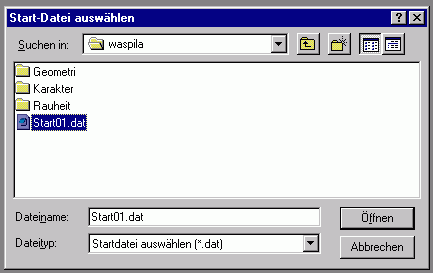
\includegraphics[width=0.8\textwidth]{waspila}
   \caption{Auswahl der Startdatei aus einem WASPILA-Projekt}
   \label{Fortgeschrittene Abb Waspila}
\end{figure}

Ausgehend von dieser Start-Datei werden in den Unterverzeichnissen GEOMETRI, KARAKTER und RAUHEIT die entsprechenden Dateien eingelesen. Der Benutzer wird dazu aufgefordert, Gew�ssername und Zustandsbezeichnung f�r eine neu anzulegende Zustandsdatei anzugeben. Sodann werden automatisch eine Zustandsdatei, sowie die Profile mit den entsprechenden Datens�tzen angelegt.

\subsubsection{Jabron}
Profildaten, die mit \wspwin{} im BCE-Format erstellt wurden, k\"{o}nnen \"{u}ber die Schnittstelle \menu{ \marrow
\underline{F}remddaten \marrow \underline{W}SPWIN--$>$JABRON} im Men\"{u} \menu{ \marrow \underline{P}rojekt} ins Datenformat
des Programms JABRON umgewandelt werden. Die Umwandlung erfolgt immer f\"{u}r eine komplette Zustandsdatei, die Sie aus Ihrem
aktuellen Projekt ausw\"{a}hlen.

Die konvertierten Daten werden im Unterverzeichnis \datei{\textbackslash prof} Ihres ge\"{o}ffneten Projektes unter dem Namen
\datei{jabron.pro} abgespeichert. Die Datei wird bei wiederholtem Aufruf des Konvertierungsprogramms stets \"{u}berschrieben.
Konvertiert werden die Datens\"{a}tze \afz{Gel\"{a}ndeh\"{o}he}, \afz{Rauheit} (unabh\"{a}ngig davon, ob es sich um $k_S$- oder
$k_{ST}$-Werte handelt), \afz{Trennfl\"{a}chen} und \afz{Durchstr\"{o}mte Bereiche}. Ebenso k\"{o}nnen Dateien im Format von JABRON
ins \wspwin{}-Format konvertiert werden.


\subsubsection{CADDY}
\wspwin{} bietet die M\"{o}glichkeit, Profilgeometrien aus dem Vermessungsprogramm CADDY zu \"{u}bernehmen. Der Import der
\datei{*.que}-Dateien erfolgt \"{u}ber den Men\"{u}punkt \menu{\marrow \underline{F}remd\-da\-ten \marrow \underline{C}ADDY}. Es
k\"{o}nnen mehrere Profile gleichzeitig in ein existierendes Projekt aufgenommen werden. Daf\"{u}r sind lediglich Zustand und
Gew\"{a}ssername anzugeben.


\subsubsection{Access}
Sie haben die M�glichkeit in \wspwin Vermessungsdaten zu importieren, die in einer ACCESS-Datenbank abgelegt wurden. Die Daten m�ssen hierzu aus ACCESS heraus als TXT-Datei exportiert werden und in folgendem Format vorliegen.

\begin{verbatim}
Datei STATION.TXT:
NR	; STATION;	GEW�SSERNAME

176,00;"53+173";"Gr. Hase"
177,00;"53+257";"Gr. Hase"
178,00;"53+332";"Gr. Hase"
179,00;"53+424";"Gr. Hase"
180,00;"53+518";"Gr. Hase"
181,00;"53+563";"Gr. Hase"
182,00;"53+611";"Gr. Hase"
183,00;"53+656";"Gr. Hase"
184,00;"53+701";"Gr. Hase"
185,00;"53+736";"Gr. Hase"
186,00;"53+807";"Gr. Hase"
187,00;"53+864";"Gr. Hase"
1,00;"00+174";"Fladderkanal"
2,00;"00+328";"Fladderkanal"
3,00;"00+530";"Fladderkanal"
4,00;"00+625";"Fladderkanal"
5,00;"00+839";"Fladderkanal"
6,00;"01+109";"Fladderkanal"
7,00;"01+369";"Fladderkanal"
8,00;"01+599";"Fladderkanal"
9,00;"01+822";"Fladderkanal"
10,00;"01+982";"Fladderkanal"
11,00;"02+063";"Fladderkanal"
\end{verbatim}

\begin{verbatim}
Datei: PROFILE.TXT
NR;	Z-Wert;	Rechtswert;	Hochwert;

1,00;24,01;3433992,90;5841859,90
1,00;23,96;3433991,30;5841862,10
1,00;24,09;3433990,50;5841863,10
1,00;23,93;3433989,40;5841864,80
1,00;23,63;3433988,40;5841865,90
1,00;22,73;3433986,90;5841868,30
1,00;22,15;3433985,50;5841870,10
1,00;21,91;3433984,80;5841871,10
1,00;21,13;3433984,40;5841871,70
1,00;20,65;3433984,10;5841872,40
2,00;24,41;3434123,70;5841941,00
2,00;24,41;3434121,60;5841944,20
2,00;24,46;3434120,30;5841946,30
2,00;24,33;3434118,60;5841948,90
2,00;24,27;3434117,60;5841950,30
\end{verbatim}

Die Daten sind wie folgt zu importieren.
W�hlen Sie aus einem ge�ffneten Projekt heraus die Men�folge: PROJEKT- FREMDDATEN- ACCESS. W�hlen Sie anschlie�end den Pfad, in dem sich die PROFILE.txt-Datei befindet und unmittelbar danach das Verzeichnis f�r Ihre STATIONEN.txt-Datei. Unter Dateiname erscheint jeweils PROFILE oder STATIONEN. Es wird f�r jedes Gew�sser eine separate Zustandsdatei angelegt, in die die Profile konvertiert werden.

\begin{figure}[hbt]
   \centering
   \includegraphics[width=0.8\textwidth]{access}
   \caption{Vermessungsdaten in einer ACCESS-Datenbank}
   \label{Fortgeschrittene Abb ACCESS Daten}
\end{figure}

\begin{figure}[hbt]
   \centering
   \includegraphics[width=0.8\textwidth]{access2}
   \caption{W�hlen der Stationen-Datei}
   \label{Fortgeschrittene Abb ACCESS Datei}
\end{figure}


\clearpage
%%%%%%%%%%%%%%%%%%%%%%%%%%%%%%%%%%%%%%%%%%%%%%%%%%%%%%%%%%%%%%%%%%%%%%%%%%%%%%%%%%%%%%%%%%%%%%%%%%%%%%%%%%%%%%%%%%%%%%%%%%%%
\section{Zust\"{a}nde bearbeiten}
%%%%%%%%%%%%%%%%%%%%%%%%%%%%%%%%%%%%%%%%%%%%%%%%%%%%%%%%%%%%%%%%%%%%%%%%%%%%%%%%%%%%%%%%%%%%%%%%%%%%%%%%%%%%%%%%%%%%%%%%%%%%

\subsection{Zust\"{a}nde kopieren}

Wenn Sie eine neue Vernetzungsdatei anlegen und einen Gew\"{a}ssernamen angeben, f\"{u}r den bereits eine Zustandsdatei existiert,
erscheint ein neuer Dialog, der Ihnen s\"{a}mtliche im Projekt vorhandenen Profildateien dieses Gew\"{a}ssers auflistet. Sie
k\"{o}nnen diese dann markieren und mit \schalter{OK} dem neuen Zustand zuordnen. Dies ist z.B. dann von Vorteil, wenn Sie
einen Istzustand und einen Planungsfall bearbeiten und bei letzterem streckenweise Profile nicht ver\"{a}ndert werden. Im
Gegensatz zu der Option \schalter{Profile aufnehmen} aus der Dialogmaske \dialog{Erfassung/Editierung der Zustandsdatei}
k\"{o}nnen hier Profile anhand ihrer Schl\"{u}sseldaten ausgew\"{a}hlt werden.

Sollten Sie keine Profile aufnehmen m\"{o}chten, so w\"{a}hlen Sie die Schaltfl\"{a}che \schalter{Abbruch}. Die Anzahl der auf diese
Weise aufnehmbaren Profile ist auf $25$ begrenzt. Sollen weitere Profile aufgenommen werden, hat dies \"{u}ber die Option
\afz{Profile aufnehmen} aus der Maske \dialog{Erfassung/Editierung der Zustandsdatei} heraus zu erfolgen (siehe
Abschnitt~\ref{Einstieg Subsec ProfilAnlegen}).

Besteht der zu kopierende Zustand aus mehr als 25~Profildateien und sind f\"{u}r den neuen Zustand nur geringe \"{A}nderungen an
den Profilen erforderlich, so kann es von Vorteil sein, zun\"{a}chst den gesamten Zustand zu kopieren. Dies geschieht mit
Hilfe des Men\"{u}s \menu{ \marrow Z\underline{u}stand \marrow Zu\underline{s}tand speichern unter}. Es erscheint die in
Abschnitt~\ref{Einstieg Subsec ProfilAnlegen} beschriebene Maske \dialog{neue Vernetzungsdatei anlegen}, in die sie den
Gew\"{a}ssernamen und den Namen des neuen Zustands eintragen m\"{u}ssen. Kopiert werden unter neuen Dateinamen alle Profile, die
Abflu{\ss}- und Verlustdatei sowie die Berechnungsvarianten.
\begin{hinweis}
   Beachten Sie, da{\ss} beim Aufnehmen von Profilen ohne Kopieren (d.h. lediglich Erstellen eines Verweises) die
   Profildateien in den beiden Zust\"{a}nden identisch sind. \"{A}nderungen am Profil im Planungsfall haben beispielsweise daher
   auch \"{A}nderungen im Istzustand zur Folge.
\end{hinweis}


\subsubsection{Beispiel - Zust�nde kopieren}

Legen Sie eine zweite Zustandsdatei f\"{u}r das Beispielgew\"{a}sser \afz{Testbach} an. Geben Sie als Gew\"{a}ssernamen \afz{Testbach}
und als Zustand \afz{Planung} an. Dazu w\"{a}hlen Sie zun\"{a}chst aus dem Dialog \dialog{Auswahl der Zustandsdatei} die
Schaltfl\"{a}che \schalter{Neue Zustandsdatei}. In den nun folgenden Dialog geben Sie ein:
\begin{quote}
   \begin{tabular}{ll}
      Gew\"{a}ssername:  &  \beisp{Testbach} \\
      Zustand:       &  \beisp{Planung}
   \end{tabular}
\end{quote}
Nach der Best\"{a}tigung der Eingabe mit \schalter{OK} \"{o}ffnet sich der Dialog, mit dessen Hilfe Sie Profildateien in den neuen
Zustand \"{u}bernehmen k\"{o}nnen. W\"{a}hlen Sie hier die erste und dritte Profildatei aus und best\"{a}tigen Sie mit \schalter{OK}. Nur
das Profil an Station $0,2~\unit{km}$ soll baulich ver\"{a}ndert werden und wird daher sp\"{a}ter kopiert oder neu erstellt.


\subsection{Strangtabelle}

Standardm\"{a}{\ss}ig wird die Strangtabelle mit einer sortierten Liste der Stationswerte aus s\"{a}mtlichen zum Zustand geh\"{o}rigen
Profilen vorbesetzt und zwar sowohl beim Neuanlegen, wie auch beim Aufnehmen oder Konvertieren von Profilen. Die
Profilabst\"{a}nde werden aus diesen Stationswerten zun\"{a}chst f\"{u}r die Vorl\"{a}nder und den Flu{\ss}schlauch einheitlich besetzt. Die
Stationwerte nehmen dabei von der M\"{u}ndung zur Quelle hin zu. \"{U}ber die Editierfelder der Strangtabelle wird die M\"{o}glichkeit
geboten, die vorgegebenen Werte zu \"{a}ndern. So k\"{o}nnen z.B. unterschiedliche Abst\"{a}nde zwischen den Profilen f\"{u}r Vorl\"{a}nder
und Flu{\ss}schlauch (z.B. bei stark m\"{a}andrierenden Gew\"{a}ssern) eingegeben werden. Die eingegebenen Werte werden auf
Plausibilit\"{a}t gepr\"{u}ft.

Die Auswahl der Profile in der Strangtabelle ist entscheidend f\"{u}r die sp\"{a}tere Wasserspiegellagenberechnung, die nur
Profile ber\"{u}cksichtigt, die durch eine Strangtabelle verkn\"{u}pft wurden. Die Strangtabelle besteht aus mehreren
Gew\"{a}sserstr\"{a}ngen, d.h. jeweils aus einem Anfangs- und einem Endprofil, wobei das Endprofil des vorherigen Stranges
zugleich das Anfangsprofil des nachfolgenden Gerinneabschnittes darstellt. Beim Eingeben der Steuerdaten f\"{u}r die
Wasserspiegellagenberechnung k\"{o}nnen hieraus eine Anfangs- und Endstation f\"{u}r die Berechnung ausgew\"{a}hlt werden. Wenn die
Strangtabelle ge\"{a}ndert wird, aber bereits Randbedingungen (Abflu{\ss}- oder Verlustdatei) und Berechnungsvarianten existieren,
werden die betroffenen Werte gel\"{o}scht.

Bei verzweigten Gerinneabschnitten und bei mehrgliedrigen Profilen kann die Strangtabelle nicht mehr automatisch
vorbesetzt werden. In diesem Fall erh\"{a}lt der Benutzer die M\"{o}glichkeit selbst festzulegen, an welcher Position der
Strangtabelle ein neues Profil einzuf\"{u}gen ist (siehe Abschnitte~\ref{Sonderprofile Subsec Mehrfeldbruecken} und
\ref{Sonderprofile Sec VerzweigteSysteme}). Beachten Sie bitte, da{\ss} beim automatischen Vorbesetzen der Strangtabelle die
Profilabst\"{a}nde aus der Differenz der Stationsangaben errechnet werden. Bei verzweigten Systemen oder starker Kr\"{u}mmung des
Flu{\ss}laufs kann daher eine Korrektur der Werte bez\"{u}glich der Profilabst\"{a}nde erforderlich sein.


\subsection{Der Umgang mit der Rauheits- und Bewuchsdatenbank}
\label{Fortgeschrittene Subsec Rauheitsdatenbank}

In \wspwin{} steht Ihnen im Grafikeditor bzw. alphanumerischen Editor f\"{u}r die Datens\"{a}tze \afz{Rauheit ks}, \afz{Rauheit
KST}, \afz{Bewuchsabst. AX in Flie{\ss}r.}, \afz{Bewuchsabst. AY quer Flie{\ss}r.}, \afz{Bewuchsdurchmesser DP} die M\"{o}glichkeit
zur Verf\"{u}gung, eine Datenbank anzulegen. Dies ist nach Wahl des entsprechenden Datensatzes \"{u}ber die Schaltfl\"{a}che
\schalter{Datenbank} im Dialogfenster \dialog{Bereiche editieren} m\"{o}glich. Die drei Datenbanken werden im Startverzeichnis
von \wspwin{} gespeichert und sind somit aus jedem Projekt heraus verf\"{u}gbar.
\begin{figure}
   \centering
   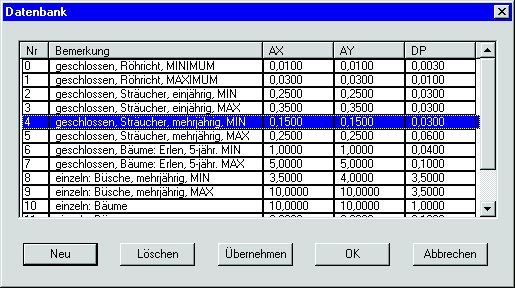
\includegraphics[width=0.9\textwidth]{DialogDatenbank}
   \caption{Bewuchsdatenbank}
   \label{Fortgeschrittene Abb Datenbank}
\end{figure}

Sollen neue Werte in die Datenbank aufgenommen werden, ist die Option \schalter{Neu} zu w\"{a}hlen. Daraufhin erhalten Sie
eine neue Zeile. Geben Sie einen Text f\"{u}r Bemerkung (maximal 40~Zeichen) ein und wechseln Sie dann per Tabulatortaste oder
Maus auf das Feld f\"{u}r die zugeh\"{o}rigen Werte.

Datenbankeintr\"{a}ge k\"{o}nnen durch Selektion des entsprechenden Listeneintrages und Bet\"{a}tigen der Schaltfl\"{a}che
\schalter{L\"{o}schen} jederzeit wieder aus der Datenbank entfernt werden. Ebenso kann der Eintrag durch Markieren und
\"{U}berschreiben der Editierfelder ge\-\"{a}n\-dert werden. Die Eintragungen werden beim Verlassen der Datenbank mit
\schalter{OK} gespeichert. \schalter{Abbruch} bewirkt ein Verlassen der Datenbank ohne Speicherung der vorgenommenen
\"{A}nderungen.

Neben dem Anlegen der Rauheitsdatenbank haben Sie auch die M\"{o}glichkeit, Werte aus der Datenbank auszuw\"{a}hlen und \"{u}ber die
Schaltfl\"{a}che \schalter{\"{U}bernehmen} direkt in eine Profildatei zu \"{u}bertragen. Nachdem Sie \schalter{\"{U}bernehmen} gew\"{a}hlt
haben, erscheint wieder die Dialogmaske \dialog{Bereiche editieren} zur Angabe des Anfangs- und Endprofilpunktes, sowie
eines Offset-, Faktor- oder neuen Wertes. Im Falle einer \"{U}bernahme von Datens\"{a}tzen aus der Datenbank ist der entsprechende
neue Wert schon eingetragen, so da{\ss} der Benutzer nur noch den Bereich einzugeben und mit \schalter{OK} zu best\"{a}tigen hat.
Bei der \"{U}bernahme von Bewuchsparametern erfolgt zus\"{a}tzlich eine Abfrage, ob alle drei Bewuchsparameter \"{u}bernommen werden
sollen. Sollte dies nicht gew\"{u}nscht sein, kann auch nur ein einzelner Parameter als aktueller Datensatz im Grafik-Editor
gew\"{a}hlt und die Frage mit \schalter{Nein} beantwortet werden. Beachten Sie, da{\ss} bei der Bewuchsdatenbank zur \"{U}bernahme von
Datens\"{a}tzen in die Profildatei die Datenblocktypen bereits angelegt sein m\"{u}ssen.




\subsection{Rauheiten global \"{a}ndern}

Die Rauheiten der einzelnen Profile k\"{o}nnen direkt im grafischen bzw. alphanumerischen Editor den einzelnen Profilen
zugeordnet werden. \wspwin{} bietet dar\"{u}ber hinaus jedoch auch noch die M\"{o}glichkeit, die Rauheiten in mehreren Profilen
gleichzeitig zu \"{a}ndern. Bedingung daf\"{u}r ist jedoch, da{\ss} der Datensatz \afz{Rauheit} bereits in den Profilen vorhanden ist.

Mit Hilfe des Men\"{u}punktes \menu{ \marrow Z\underline{u}stand \marrow \underline{R}auheiten \"{a}ndern} gelangen Sie in einen
Dialog (Abbildung~\ref{Fortgeschrittene Abb DialogRauheitenAendern}), in dem sie jedem Profil eine neue Rauheit f\"{u}r das
linkes Vorland, den Flu{\ss}schlauch und das rechte Vorland zuweisen k\"{o}nnen.
\begin{figure}
   \centering
   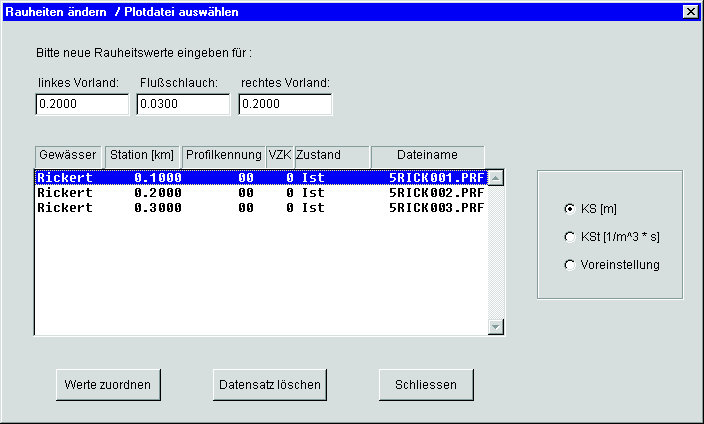
\includegraphics[width=1.0\textwidth]{DialogRauheitenAendern}
   \caption{Dialogfenster Rauheiten \"{a}ndern}
   \label{Fortgeschrittene Abb DialogRauheitenAendern}
\end{figure}
Durch Festhalten der \schalter{Strg}-Taste k\"{o}nnen mehrere Profile gleichzeitig mit der Maus ausgew\"{a}hlt werden. Die Eingabe
der neuen Rauheiten erfolgt in die daf\"{u}r vorgesehenen Felder oberhalb der Profilauswahltabelle. \"{U}ber die Schaltfl\"{a}che
\schalter{Werte zuordnen} werden die neuen Rauheiten in die Profildateien \"{u}bernommen. Es erfolgt eine Abfrage, ob sie
weitere Profile bearbeiten m\"{o}chten. Sie k\"{o}nnen auch das Protokoll zur Bearbeitung der Profildateien einsehen.

Die Schaltfl\"{a}che \schalter{Datensatz l\"{o}schen} hat die gleiche Funktion wie im alphanumerischen und im grafischen Editor.
Der Datensatz \afz{Rauheit} kann hier in den ausgew\"{a}hlten Profilen komplett gel\"{o}scht werden. Das Auswahlfeld auf der
rechten Seite erlaubt Ihnen einen anderen Rauheitsdatensatz auszuw\"{a}hlen.



\subsection{Die Eingabe von Einzelverlusten}
\label{Fortgeschrittene Subsec Einzelverluste}

Der Ber\"{u}cksichtigung von Str\"{o}mungsverlusten kommt bei der Berechnung von Wasserspiegellagen eine erhebliche Bedeutung zu.
Prinzipiell wird zwischen kontinuierlich zunehmenden (Wandreibungsverlust) und \"{o}rtlich konzentrierten Verlusten
unterschieden. Der Wandreibungsverlust wird \"{u}ber entsprechende Reibungsans\"{a}tze im Flie{\ss}gesetz be\-r\"{u}ck\-sichtigt. Die
Einzelverluste lassen sich durch den allgemeinen Verlustansatz in der Hydraulik erfassen:
\begin{equation}
   H_{ZV} = \zeta \cdot \frac{v_{i-1}^2}{2g}
      \label{Fortgeschrittene Gl Einzelverluste}
\end{equation}
Der Verlustbeiwert $\zeta$ ist abh\"{a}ngig von der Art und der Form der St\"{o}rstelle.

\subsubsection{Ber\"{u}cksichtigung der Erweiterungsverluste nach dem Ansatz von \autor{Borda-Carnot}}
Die Verlusth\"{o}he infolge einer Aufweitung des Querschnitts kann nach \autor{Borda-Carnot} wie folgt bestimmt werden:
\begin{equation}
   H_{ZV} = c_i \cdot \frac{(v_i - v_{i-1})^2}{2g}
      \label{Fortgeschrittene Gl VerlustBordaCarnot}
\end{equation}
Dabei stellen $v_i$ und $v_{i-1}$ jeweils die mittleren Geschwindigkeiten im Gesamtquerschnitt dar. Der Faktor $c_i$ ist
ein frei zu w\"{a}hlender Abminderungsfaktor.

\subsubsection{Verengungsverluste}
Der Verlustbeiwert bei Verengungen kann f\"{u}r Kompaktquerschnitte in erster N\"{a}herung aus dem Fl\"{a}chenverh\"{a}ltnis abgesch\"{a}tzt
werden:
\begin{equation}
   \zeta_E = c_i \cdot \left(\frac{A_{i-1}}{A_i} - 1 \right)^2
      \label{Fortgeschrittene Gl Verengungsverluste}
\end{equation}
Die Verlusth\"{o}he erh\"{a}lt man dann mit Hilfe von Gleichung~\ref{Fortgeschrittene Gl Einzelverluste}.

\subsubsection{Dateneingabe in der Verlustdatei}
Die Verlustbeiwerte werden (wie auch die Abflu{\ss}daten) in einer separaten Verlustdatei gespeichert. \"{U}ber das Men\"{u}
\menu{\marrow Z\underline{u}stand \marrow Einzel\underline{v}erluste} \"{o}ffnen Sie den Dialog zur Eingabe der erforderlichen
Beiwerte.
\begin{figure}[hbt]
   \centering
   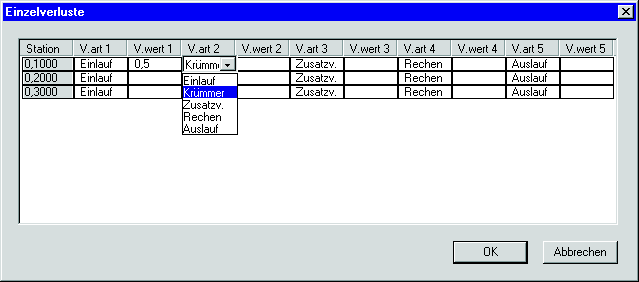
\includegraphics[width=1.0\textwidth]{Verlustdatei}
      \caption{Dialogfenster zur Eingabe der Parameter in die Verlustdatei}
      \label{Fortgeschrittene Abb Verlustdatei}
\end{figure}

An jeder Station k\"{o}nnen bis zu f\"{u}nf verschiedene Beiwerte eingegeben werden. Neben jedem Wertefeld finden Sie eine Liste
aus der sie die entsprechende Verlustart ausw\"{a}hlen k\"{o}nnen. Die Eingabe der Verlustart hat keinen Einflu{\ss} auf die
Berechnung, Sie dient lediglich Ihrer Information.

Die Interpretation der eingegebenen Werte vom Programm ist abh\"{a}ngig von den Festlegungen bei der Eingabe der
Steuerparameter f\"{u}r die Berechnung. Weitere Informationen hierzu finden Sie in Abschnitt~\ref{Fortgeschrittene Subsec
Einstellungen} dieses Handbuchs.

Prinzipiell sind die \"{o}rtlichen Verlustbeiwerte $\zeta$ jeweils im oberstromigen Profil einzugeben. Dies gilt auch f\"{u}r
Verluste an Verengungen im Br\"{u}ckenbereich. Soll der Verengungsverlust nach Gleichung~\ref{Fortgeschrittene Gl
Verengungsverluste} automatisch berechnet werden, so ist dies durch die Eingabe eines negativen Wertes an der betreffenden
Station zu kennzeichen. Der negative Wert wird dann bei entsprechender Vereinbarung in den Steuerdaten der Berechnung als
Abminderungsfaktor $c_i$ interpretiert. Die Eingabe eines positiven Wertes kann in Abh\"{a}ngigkeit von den in
Abschnitt~\ref{Fortgeschrittene Subsec Einstellungen} zu treffenden Vereinbarungen f\"{u}r die Berechnung sowohl als \"{o}rtlicher
Verlustbeiwert $\zeta$ nach Gleichung~\ref{Fortgeschrittene Gl Einzelverluste} (keine automatische Berechnung von
Einzelverlusten) als auch als Abminderungsfaktor $c_i$ f\"{u}r die automatische Ber\"{u}cksichtigung der Erweiterungsverluste nach
Gleichung~\ref{Fortgeschrittene Gl VerlustBordaCarnot} gedeutet werden.



\subsection{Vergleich von Zust\"{a}nden und Profilen}
\label{Fortgeschrittene Subsec Vergleichszustaende}

Sie k\"{o}nnen mit Hilfe von \wspwin{} Vergleiche zwischen einzelnen Zust\"{a}nden hinsichtlich Fl\"{a}chen- und Massenberechnung
vornehmen. Voraussetzung daf\"{u}r ist, da{\ss} bei den zu vergleichenden Profilen neben dem Gew\"{a}ssernamen und der Station auch
jeweils erste und letzte Profilpunkt (Gel\"{a}ndekoordinaten) \"{u}bereinstimmt.

\subsubsection{Vergleich der Gel\"{a}ndekontur}
Ihr aktueller Zustand bildet f\"{u}r den Vergleich den Referenzzustand. F\"{u}r den Vergleich des kompletten Zustandes mu{\ss} die
Dialogmaske \dialog{Erfassung/Editierung der Zustandsdatei} ge\"{o}ffnet sein. \"{U}ber das Men\"{u} \menu{\marrow Z\underline{u}stand
\marrow Ver\underline{g}leichszutand \marrow \underline{G}el\"{a}nde \marrow \underline{n}eu} k\"{o}nnen sie Ihren
Vergleichszustand ausw\"{a}hlen. In den Profildateien Ihres Referenzzustandes wird nun der Datensatz \afz{2. Gel\"{a}nde H\"{o}he} mit
den Gel\"{a}ndedaten aus dem Vergleichszustand angelegt.

Bei der Auswahl des Datensatzes im Grafikeditor werden nun sowohl die Gel\"{a}ndekontur des Referenzzustandes, als auch die
Gel\"{a}ndekontur des Vergleichszustandes angezeigt. Der Datensatz \afz{2.Gel\"{a}nde H\"{o}he} kann \"{u}ber das Untermen\"{u} \menu{\marrow
\underline{G}el\"{a}nde \marrow \underline{l}\"{o}schen} wieder aus allen Profilen des Referenzzustandes entfernt werden.

\subsubsection{Fl\"{a}chenberechnung}
Neben dem reinen Verkn\"{u}pfen der Profile aus zwei geometrischen Zust\"{a}nden (d.h. der parallelen Darstellung von zwei
Gel\"{a}ndeh\"{o}hen in den Profilen) kann auch eine Fl\"{a}chenberechnung des Auf- und Abtrags zwischen den Profilen zweier zu
vergleichender Zust\"{a}nde durchgef\"{u}hrt werden.

Die zustandsbezogene Fl\"{a}chenberechnung erfolgt analog der Gel\"{a}ndeverkn\"{u}pfung \"{u}ber die Men\"{u}folge \menu{\marrow
Z\underline{u}stand \marrow Ver\underline{g}leichszustand \marrow \underline{F}l\"{a}che \marrow \underline{n}eu}. F\"{u}r alle
Profile, deren Stationen im Referenz- und Vergleichszustand identisch sind und bei denen der erste und letzte Profilpunkt
\"{u}bereinstimmen, werden die Datens\"{a}tze \afz{2.Gel\"{a}nde H\"{o}he} und \afz{Fl\"{a}che} angelegt, nachdem \"{u}ber die bekannte
Dialogmaske ein Vergleichszustand ausgew\"{a}hlt wurde. Sollte bereits eine Gel\"{a}ndeverkn\"{u}pfung oder Fl\"{a}chenberechnung
existieren, erscheint zun\"{a}chst die Abfrage, ob die alte Verkn\"{u}pfung zu l\"{o}schen ist, oder ob die bereits existierende
Gel\"{a}ndeverkn\"{u}pfung der Fl\"{a}chenberechnung zugrundegelegt werden soll. Falls Sie sich unschl\"{u}ssig sind, k\"{o}nnen Sie den
Vorgang auch \"{u}ber die Option \schalter{Abbrechen} beenden.

Nachdem Sie eine Fl\"{a}chenberechnung erfolgreich durchgef\"{u}hrt haben, k\"{o}nnen Sie den berechneten Auf- und Abtrag f\"{u}r jedes
Profil im alphanumerischen bzw. grafischen Editor betrachten. Der Datensatz \afz{Fl\"{a}che} enth\"{a}lt die einzelnen
Fl\"{a}chenwerte. Diese beziehen sich jeweils auf den Bereich rechts vom zugeh\"{o}rigen $y$-Wert. Positive Werte charakterisieren
dabei Auftrags- und negative Abtragsfl\"{a}chen. Neben den Einzelwerten werden in einem zus\"{a}tzlichen Fenster jeweils die
Summen des Auf- und Abtragsfl\"{a}chen, sowie die Gesamtsumme der Fl\"{a}chendifferenz ausgegeben. Der in allen Profilen
eingef\"{u}gte Datensatz \afz{Fl\"{a}che} kann wiederum \"{u}ber das Untermen\"{u} \menu{ \marrow \underline{F}l\"{a}che \marrow
\underline{l}\"{o}schen} aus allen Profildateien des Referenzzustandes entfernt werden.

\subsubsection{Vergleich einzelner Profile}
In gleicher Weise wie der Vergleich der Gel\"{a}ndekontur und die Fl\"{a}chenberechnung f\"{u}r komplette Zust\"{a}nde erfolgen kann, ist
es auch m\"{o}glich nur einzelne Profildateien verschiedener Zust\"{a}nde zu vergleichen. Auch hier m\"{u}ssen Anfangs- und Endpunkt
der Gel\"{a}n\-dekoordinaten, sowie die Station und der Gew\"{a}ssername \"{u}bereinstimmen. Der Aufruf erfolgt hierbei \"{u}ber das Men\"{u}
\menu{ \marrow Z\underline{u}stand \marrow Ver\underline{g}leichszutand} aus dem grafischen oder alphanumerischen Editor
heraus. Die weitere Vorgehensweise entspricht dem Vergleich zweier kompletter Zust\"{a}nde.


\subsection{Profile verl\"{a}ngern}
\wspwin{} ist in der Lage, bereits existierende Profile mit weiteren Profilen zu verl\"{a}ngern, d.h. diese links oder rechts
an das aktuelle Profil anzuh\"{a}ngen. Die Option kann dann von Interesse sein, wenn Profile oder Vorl\"{a}nder nachvermessen
werden oder weitere Daten z.B. aus einem digitalen H\"{o}henmodell vorliegen, die an das bereits existierende Profil
angebunden werden sollen.

W\"{a}hlen Sie hierzu aus dem alphanumerischen oder grafischen Editor heraus die Option \schalter{Profil verl\"{a}ngern}. Sie
werden dazu aufgefordert eine Profildatei im \wspwin{}- oder BCE-Format (\datei{*.prf} / \datei{*.dat}) auszuw\"{a}hlen, mit
der ihre aktuelle gerade dargestellte Profildatei zu verl\"{a}ngern ist. Anschlie{\ss}end m\"{u}ssen Sie noch angeben, ob das
ausgew\"{a}hlte Profil links oder rechts angef\"{u}gt werden soll.


\subsection{Profile interpolieren}

Bei zu gro{\ss} gew\"{a}hlten Profilabst\"{a}nden, insbesondere bei einem Flie{\ss}wechsel, k\"{o}nnen Zwischenprofile erforderlich werden.
Daf\"{u}r bietet \wspwin{} die M\"{o}glichkeit der Profilinterpolation. In dem Men\"{u} \menu{\marrow Z\underline{u}stand} finden sie
den Unterpunkt \menu{ \marrow \underline{I}nterpolieren}.
\begin{figure}[hbt]
   \centering
   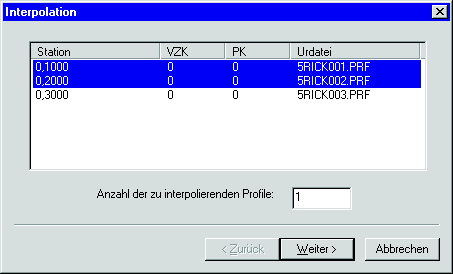
\includegraphics[width=0.8\textwidth]{Profilinterpolation1}
   \\[12pt]
   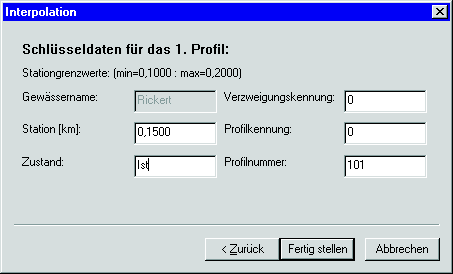
\includegraphics[width=0.8\textwidth]{Profilinterpolation2}
   \caption{Assistent zur Durchf\"{u}hrung von Profilinterpolationen}
   \label{Fortgeschrittene Abb Profilinterpolation}
\end{figure}

Mit seiner Hilfe gelangen sie in das Dialogfenster Abbildung~\ref{Fortgeschrittene Abb Profilinterpolation} oben. Hier
werden Sie zur Auswahl der Profile aufgefordert, zwischen denen interpoliert werden soll. Die Anzahl der einzuf\"{u}genden
Profile mu{\ss} in dem Feld \feld{Anzahl der zu interpolierenden Profile} eingegeben werden. Die Schaltfl\"{a}che
\schalter{Weiter} f\"{u}hrt sie in das nachfolgende Dialogfenster (Abbildung~\ref{Fortgeschrittene Abb Profilinterpolation},
unten), in dem Sie zur Festlegung der Schl\"{u}sseldaten entsprechend Abschnitt~\ref{Einstieg Subsec ProfilAnlegen} f\"{u}r das zu
interpolierende Profil aufgefordert werden. Entsprechend ihrer vorher gew\"{a}hlten Anzahl einzuf\"{u}gender Profile wiederholt
sich dieser Dialog. Die Profilinterpolation kann nicht bei Profilen mit R\"{u}ckspr\"{u}ngen (\autor{Gauss}-Profile) angewendet
werden.



\clearpage
%%%%%%%%%%%%%%%%%%%%%%%%%%%%%%%%%%%%%%%%%%%%%%%%%%%%%%%%%%%%%%%%%%%%%%%%%%%%%%%%%%%%%%%%%%%%%%%%%%%%%%%%%%%%%%%%%%%%%%%%%%%%
\section{Weitere Berechnungsoptionen}
%%%%%%%%%%%%%%%%%%%%%%%%%%%%%%%%%%%%%%%%%%%%%%%%%%%%%%%%%%%%%%%%%%%%%%%%%%%%%%%%%%%%%%%%%%%%%%%%%%%%%%%%%%%%%%%%%%%%%%%%%%%%

\subsection{Zus\"{a}tzliche Berechnungsm\"{o}glichkeiten}

\begin{figure}[hbt]
   \centering
   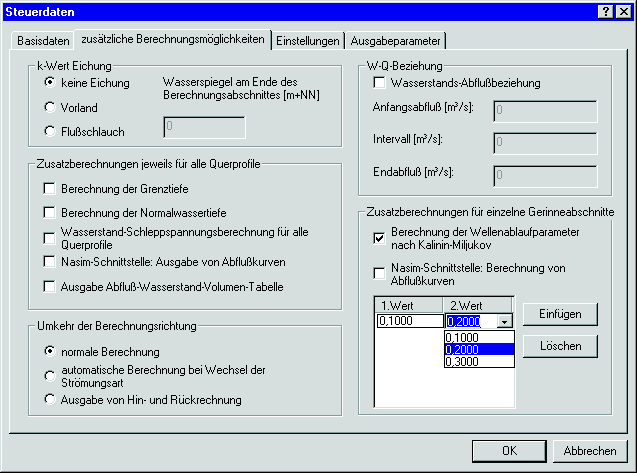
\includegraphics[width=1.0\textwidth]{ZusaetzlicheBerechnungsmoeglichkeiten}
   \caption{Registerkarte \dialog{Zus\"{a}tzliche Berechnungsm\"{o}glichkeiten}}
   \label{Fortgeschrittene Abb ZusaetzlicheBerechnungsmoeglichkeiten}
\end{figure}


\subsubsection{Eichung von Rauheitswerten}
Zur Bestimmung eines mittleren Rauheitsbeiwertes aus Me{\ss}werten (Kalibrierung) ist im Rechenprogramm folgendes
Verfahren~\cite{FelkelCanisius} zugrundegelegt:

Ausgehend von einer bekannten hydraulischen Randbedingung (Anfangswasserstand) wird die Wasserspiegellinie zun\"{a}chst mit
einem gesch\"{a}tzten Rauheitsbeiwert berechnet. Anschlie{\ss}end wird verglichen, ob der berechnete Endwasserspiegel mit dem
beobachteten \"{u}bereinstimmt. Ist dies nicht der Fall, so wird die Spiegellinienberechnung mit einem verbesserten
Rauheitsbeiwert wiederholt. Dieser Iterationsvorgang wird abgebrochen, wenn die Differenz zwischen vorgegebenem und
berechnetem Endwasserstand die gew\"{u}nschte Genauigkeitsschranke unterschreitet. Das Ergebnis ist ein mittlerer
Rauheitsbeiwert f\"{u}r den gew\"{a}hlten Abschnitt.

Im Falle gegliederter Querschnitte ist zun\"{a}chst der Rauheitsbeiwert des Flu{\ss}schlauchs f\"{u}r ein etwa bordvolles Hochwasser
zu bestimmen. Erst dann kann f\"{u}r ein ausuferndes Hochwasser der mittlere Rauheitsbeiwert der Vorlandfl\"{a}chen berechnet
werden.

Zur Eichung einer Flu{\ss}strecke kann jeder Flu{\ss}abschnitt gew\"{a}hlt werden, in dem \emph{kein} Flie{\ss}wechsel auftritt und in dem
gleichbleibende Rauheitsstrukturen vorliegen. F\"{u}r Strecken mit durchstr\"{o}mtem Bewuchs liegen noch keine brauchbaren
Kalibrierungsalgorithmen vor, d.h. eine Kalibrierung ist nur durch gezielte Vorgabe einzelner Rauheitsparameter m\"{o}glich.

Die berechneten Wasserspiegelh\"{o}hen der Kalibrierungsrechnung sind mit den gemessenen Wasserst\"{a}nden der Gesamtstrecke zu
vergleichen. Sollte keine befriedigende \"{U}bereinstimmung \"{u}ber den gesamten Bereich vorhanden sein, so ist eine Aufteilung
in mehrere Berechnungsabschnitte erforderlich. Die Rauheitsbeiwerte k\"{o}nnen im Extremfall in jedem Querprofil andere Werte
annehmen. (In derartigen F\"{a}llen ist eine Optimierung der Rauheitsbeiwerte nach \cite{SeusUslu} zu empfehlen.)

Die Dateneingabe bei der Eichung von Rauheitsbeiwerten erfolgt genauso wie bei einer normalen
Wasserspiegellagenberechnung. Die (notwendigen) Anfangswerte der $k_S$- bzw. $k_{ST}$-Werte sind als Startwerte zu
sch\"{a}tzen und werden in den Profildateien eingegeben. Beim Editieren der Steuerdaten f\"{u}r die Berechnung wird zus\"{a}tzlich zum
gemessenen Anfangswasserstand (mu{\ss} als Direkteingabe erfolgen) der ebenfalls gemessene Wasserstand des Zielprofils als
Wasserspiegel am Ende des Berechnungsabschnittes eingetragen. Weiterhin mu{\ss} angegeben werden, ob die Eichung im Flu{\ss}bett
oder f\"{u}r die Vorl\"{a}nder erfolgen soll.

Bei Wahl der Flie{\ss}gesetze nach \autor{Manning-Strickler} und \autor{Prandtl-Colebrook} werden einheitliche $k$-Werte,
getrennt f\"{u}r den Flu{\ss}schlauch und die Vorl\"{a}nder berechnet, g\"{u}ltig f\"{u}r den gesamten Berechnungsabschnitt vom
Anfangswasserspiegel bis zum Endwasserspiegel. Bei unterschiedlichen Rauheitswerten im Querprofil lassen sich einzelne
Werte in den Profildateien durch ein Minuszeichen von der Eichung ausnehmen. Ansonsten erfolgt die Kalibrierung unter
Beibehaltung der eingegebenen Rauheitsbeiwertabstufung, d.h. alle Ausgangswerte werden mit dem gleichen Korrekturfaktor
ver\"{a}ndert. Auch hier ist eine Differenzierung erforderlich: Zuerst sollte der $k$-Wert des bordvollen Abflusses f\"{u}r den
Flu{\ss}schlauch geeicht werden, danach ist ggf. eine Eichung f\"{u}r $k$-Werte der Vorl\"{a}nder sinnvoll.

Bei Auswahl von Berechnungsans\"{a}tzen, die unterschiedliche Rauheiten im Teilabflu{\ss}querschnitt ber\"{u}cksichtigen, werden die
neuen $k$-Werte nicht in den Ergebnislisten (dort erscheinen nur die Widerstandsbeiwerte $\lambda_j$) gespeichert. Die
Speicherung erfolgt in neuen \datei{*.WSP}-Dateien, die zur anschlie{\ss}enden Weiterverarbeitung als neue Eingabedateien
verwendet werden k\"{o}nnen. Das hei{\ss}t, die Dateien k\"{o}nnen \"{u}ber die Option \menu{\marrow \underline{P}rojekt \marrow
\underline{F}remddaten \marrow \underline{H}YDRAWSP} ins \wspwin{}-Format zur\"{u}ckkonvertiert werden. Der Dateiname
entspricht dem Namen der zugrunde gelegten Berechnungsvariante, wobei die 3., 4. und 5. Buchstaben \datei{*wkw*.*} lauten.
\begin{quote}
   \begin{tabular}{lll}
         Beispiel:   &  Ursprungsdatei:      &  \datei{ri000001.001} \\
                     &  neue $k$-Werte in:   &  \datei{riwkw001.001}
   \end{tabular}
\end{quote}
\begin{hinweis}
   Legen Sie nach M\"{o}glichkeit f\"{u}r die Rauheitseichung eine extra Berechnungsvariante an, in der keine zus\"{a}tzlichen
   Steueroptionen au{\ss}er den zwingend n\"{o}tigen angegeben sind. Bei der Wahl zu vieler verschiedener Steueroptionen in einer
   Variante k\"{o}nnen u.U. Probleme auftreten.
\end{hinweis}


\subsubsection{Schiessender Abflu{\ss}}
Die \autor{Froude}'sche Zahl $\mathit{Fr}$ ist ein Kriterium daf\"{u}r, ob ein Abflu{\ss} str\"{o}mend, mit kritischer Tiefe oder
schie{\ss}end erfolgt. W\"{a}hrend der Berechnung der Wasserspiegellinie wird die zu jeder diskreten Wasserspiegellage geh\"{o}rende
\autor{Froude}'sche Zahl ermittelt. Wenn sich zwischen zwei Querprofilen der Flie{\ss}zustand \"{a}ndert, wird dies durch die
\autor{Froude}'sche Zahl angezeigt. Hierbei sind zwei F\"{a}lle zu unterscheiden:
\begin{enumerate}
   \item Der Flie{\ss}wechsel wird durch eine \"{o}rtlich begrenzte Engstelle erzwungen, der Flie{\ss}zustand oberhalb ist
         wieder str\"{o}mend. Hierbei ist von Bedeutung, da{\ss} der Abflu{\ss} bei $\mathit{Fr} = 1,0$ mit minimaler Energie erfolgt.
         Bei einem verbauten Querschnitt oder einer \"{o}rtlich begrenzten Unstetigkeit im Flu{\ss}lauf mu{\ss} in jedem Fall die
         Grenztiefe durchlaufen werden, wenn ein Flie{\ss}wechsel erzwungen wird. Die Berechnung des Wasserspiegels f\"{u}r das
         Profil oberhalb der Engstelle erfolgt dann mit Hilfe des Extremalprinzips von \autor{B\"{o}ss-Belanger}
         (\cite{PressSchroeder}, S.~239). Das Prinzip besteht in einer speziellen Anwendung der \autor{Bernoulli}'schen
         Gleichung, wobei (wie im str\"{o}menden Zustand) ein Energieh\"{o}henvergleich zwischen zwei Querschnitten vorgenommen
         wird, von denen der eine durch den Sonderfall des Energieminimums ausgezeichnet ist.

         Die Reibungsverluste f\"{u}r die Flie{\ss}strecke zwischen den beiden Querschnitten werden abweichend von der sonst
         \"{u}blichen Regel nicht durch Mittelung der Reibungsgef\"{a}lle berechnet, da eine \"{U}bertragung der Engstellengeometrie
         auf die oberwasserseitige Flie{\ss}strecke meist unzutreffend ist. Bei einer \"{o}rtlichen Engstelle beschreibt das
         oberwasserseitige Energieliniengef\"{a}lle die Verh\"{a}ltnisse zutreffender, deshalb wird im Programm nur mit dem
         oberwasserseitigen Energieliniengef\"{a}lle gerechnet. Zur Vermeidung von Fehlern darf im kritischen Abflu{\ss}bereich
         in keinem Fall mit zu gro{\ss}en Abst\"{a}nden der Querprofile gerechnet werden. Der zus\"{a}tzliche Energieverlust durch
         die Einschn\"{u}rung der Stromlinien im Einlauf zur Engstelle kann als \"{o}rtlicher Verlust entsprechend
         Abschnitt~\ref{Fortgeschrittene Subsec Einzelverluste} erfa{\ss}t werden. Ein Flie{\ss}wechsel in der Engstelle liegt
         vor, wenn die Energieh\"{o}he im Profil~($i$) bei $\mathit{Fr} = 1,0$ gr\"{o}{\ss}er ist als die im Unterwasser vorhandene
         Energieh\"{o}he.
         \begin{equation}
            \mathit{min}H_{E,i} > H_{E,i-1} + h_R
         \end{equation}

   \item Es findet ein \"{U}bergang zu einem schie{\ss}enden Normalabflu{\ss} statt, d. h. der Flie{\ss}zustand bleibt auch in den
         nachfolgenden Profilen im schie{\ss}enden Bereich. Ob dieser Fall vorliegt, kann durch eine \"{U}berpr\"{u}fung der
         \autor{Froude}-Zahl im Oberwasserbereich festgestellt werden.

         Wenn mindestens zwei aufeinanderfolgende
         Querschnitte im schie{\ss}enden Bereich liegen, werden f\"{u}r die flu{\ss}aufw\"{a}rts liegenden Querprofile solange die
         querschnittsspezifischen kritischen Wassertiefen berechnet und ausgedruckt, bis sich wieder ein str\"{o}mender
         Flie{\ss}zustand ergibt.
\end{enumerate}

\newpage
\begin{hinweis}
   Die bei einem Wechsel in den anderen Flie{\ss}zustand ausgegeben kritischen Wasserspiegellagen sind nur als obere
   Grenzwerte des schie{\ss}enden Str\"{o}mungsabschnittes  anzusehen. Zur Berechnung der genauen Spiegellagen im schie{\ss}enden
   Bereich ist ein gesonderter Berechnungslauf mit Angabe der oberwasserseitigen hydraulischen Randbedingung oder einem
   automatischen Wechsel der Berechnungsrichtung erforderlich.
\end{hinweis}

Eine automatische Berechnung der richtigen (schie{\ss}enden) Wasserspiegellagen setzt nicht nur eine Umkehrung der
Berechnungsrichtung, sondern in den meisten F\"{a}llen auch wesentlich kleinere Profilabst\"{a}nde voraus. Oft ist beim
nat\"{u}rlichen Abflu{\ss} im schie{\ss}enden Bereich kein Energiegleichgewicht zwischen den willk\"{u}rlich gew\"{a}hlten Profilstationen
vorhanden. Hier reicht zumeist die Absch\"{a}tzung der schie{\ss}enden Normalwassertiefen aus, die einen guten Anhalt f\"{u}r die
voraussichtlichen Wasserst\"{a}nde liefern. F\"{u}r eine erste Absch\"{a}tzung der Wasserst\"{a}nde bei wechselnden Flie{\ss}zust\"{a}nden ist
eine automatische Umkehrung der Berechnungsrichtung f\"{u}r Teilstrecken im schie{\ss}enden Bereich im Programm vorgesehen. Bei
der Dateneingabe kann der schie{\ss}ende Abflu{\ss} mit einer Umkehr der Str\"{o}mungsrichtung an folgenden Stellen optional
ber\"{u}cksichtigt werden:
\begin{itemize}
   \item bezogen auf den Anfangswasserspiegel
   \begin{itemize}
      \item Ber\"{u}cksichtigung des schie{\ss}enden Abflusses beim Anfangswasserspiegel,
      \item Umkehr der Berechnungsrichtung, das Startprofil f\"{u}r die Berechnung ist das Profil am Ende der
            Berechnungsstrecke (Oberwasser).
   \end{itemize}
   \item Bezogen auf den gesamten Berechnungsabschnitt
   \begin{itemize}
      \item normale Berechnung, Standardeinstellung,
      \item keine automatische Umkehr der Berechnungsrichtung bei Wechsel der Str\"{o}\-mungs\-art
      \item automatische Umkehr der Berechnungsrichtung bei Wechsel der Str\"{o}mungsart
      \item Ausgabe von Hin- und R\"{u}ckrechnung
   \end{itemize}
\end{itemize}


\subsubsection{Berechnung der Grenztiefe f\"{u}r alle Profile}
Wenn Sie zus\"{a}tzlich zu Ausgabe der Wasserspiegellagen und den hydraulischen Parametern in der Ergebnisdatei eine Ausgabe
der kritischen Wassertiefe w\"{u}nschen, k\"{o}nnen Sie das optional zu bet\"{a}tigende Kontrollk\"{a}stchen \checkbox{Berechnung der
Grenztiefe f\"{u}r alle Profile} markieren. Es werden dann zwei Berechnungen durchgef\"{u}hrt, deren Ergebnisse in der
Ergebnisdatei hintereinander dargestellt sind. Die erste Berechnung enth\"{a}lt die Ergebnisse Ihrer Berechnungsvariante, die
zweite gibt die Grenztiefen, mit den zugeh\"{o}rigen hydraulischen Parametern wieder.

\subsubsection{Berechnung der Normalwassertiefe f\"{u}r alle Profile}
In gleicher Weise wie f\"{u}r die Grenztiefe kann auch eine Berechnung der Normalwassertiefen in allen Profilen durchgef\"{u}hrt
werden. Dabei werden ebenfalls zwei Berechnungen ausgef\"{u}hrt. Die Ergebnisse der zweiten Berechnungsvariante spiegeln jetzt
jedoch den station\"{a}r gleichf\"{o}rmigen Abflu{\ss} mit den Normalwassertiefen wieder.

\subsubsection{Wasserstand-Schleppspannungsberechnung in allen Profilen}
Die Schleppspannungen $\tau$~[$\unit{N/m^2}$] werden nach \cite{PressSchroeder, DtForschungsgem} als Sohlschubspannung f\"{u}r
jeden Teilabflu{\ss}querschnitt getrennt berechnet.
\begin{equation}
   \tau = \gamma \cdot r_{hy} \cdot I_E
\end{equation}
Der hydraulische Radius $r_{hy}$ ergibt sich nach Gleichung~\ref{Einstieg Gl HydraulRadius}. Das spezifische Gewicht
$\gamma$ von Wasser betr\"{a}gt $10\unit{kN/m^3}$. Zur Kontrolle der Schleppspannungen im Flu{\ss}lauf werden in der Ergebnisdatei
untereinander zwei Tabellen erzeugt:
\begin{itemize}
   \item Geschwindigkeiten und Schleppspannungen in den Profilen
   \item Abschnittsweise Schleppspannungen
\end{itemize}
Die abschnittsweisen Schleppspannungen ergeben sich als Mittelwerte aus den profilweise berechneten Werten. Hierbei sind
kontinuierliche \"{U}berg\"{a}nge zwischen den Querschnittsabmessungen vorausgesetzt. W\"{a}hlt man die Option
\checkbox{Wasserstand-Schleppspan\-nungberechnung f\"{u}r alle Profile}, wird f\"{u}r jedes Querprofil und jeden Strang eine
Tabelle mit Abflu{\ss}, Wasserstand sowie Geschwindigkeiten und Schleppspannungen in den Teilabflu{\ss}querschnitten ausgegeben.

\subsubsection{Nasim-Schnittstelle: Ausgabe von Abflu{\ss}kurven}
Bei der hydrologischen Langzeitsimulation nach NASIM oder LWANAS (SMO-Konzept in NRW) besteht die M\"{o}glichkeit, statt mit
repr\"{a}sentativen Querprofilen, mit sogenannten Abflu{\ss}kurven zu rechnen. Von Bedeutung ist hierbei, da{\ss} nicht nur Rechenzeit
zur Aufstellung der Abflu{\ss}kurven f\"{u}r die Ersatzprofile eingespart wird, sondern die hydraulisch berechneten
\afz{Abflu{\ss}kurven} werden aus dem Retentionsvolumen berechnet, d.h. eigentlich handelt es sich um Volumenkurven, die durch
Vorgabe einer fiktiven Abflu{\ss}breite zu Abflu{\ss}kurven transformiert werden.

Die Option \checkbox{Nasim-Schnittstelle: Ausgabe von Abflu{\ss}kurven} gibt die Abflu{\ss}kurven aller Querprofile f\"{u}r die
Weiterverwendung in hydrologischen Simulationsprogrammen (z.B. NASIM) aus. Es ist auch m\"{o}glich nur bestimmte Abschnitte
der Berechnungsstrecke auszugeben. In diesem Falle ist die Checkbox \checkbox{Nasim-Schnittstelle: Ausgabe von
Abflu{\ss}kurven} im Bereich \dialog{Zusatzberechnungen f\"{u}r einzelne Gerinneabschnitte} zu markieren. In der kleinen Tabelle
darunter (Abbildung~\ref{Fortgeschrittene Abb ZusaetzlicheBerechnungsmoeglichkeiten} unten rechts) k\"{o}nnen dann die Str\"{a}nge
definiert werden, f\"{u}r die die Abflu{\ss}kurven ausgegeben werden sollen. Mit Hilfe der Schaltfl\"{a}che \schalter{Einf\"{u}gen}
erstellen sie einen neuen Strang. Beim Klick in die Tabelle erscheint ein Listenfeld mit allen Stationsangaben. W\"{a}hlen Sie
hier den Strang aus und verfahren Sie analog mit den restlichen Str\"{a}ngen des Berechnungsabschnitts. Durch
\schalter{L\"{o}schen} lassen sich Str\"{a}nge wieder aus der Tabelle entfernen.

Die Ergebnisse werden im Projektunterverzeichnis~\datei{...\textbackslash dath} in eine Datei geschrieben. Der dritte und
vierte Buchstabe des Dateinamens lautet bei der Ausgabe einzelner Str\"{a}nge \datei{*n5*.*}, ansonsten \datei{*n6*.*}. Als
Beispiel sind hier die Dateinamen der Schnittstellendateien einer Berechnung an der Fulda dargestellt:
\begin{quote}
   \datei{fun50001.001} \quad einzelne Abschnitte \\
   \datei{fun60001.001} \quad alle Profile
\end{quote}
Der Datei \datei{*n5*.*}liegt folgendes Format zugrunde (s. NASIM-Dokumentation Jan. 1988, Seite C-28):
\begin{center}
   \begin{tabular}{p{1.2cm}p{1.2cm}p{1.2cm}p{1.5cm}p{5cm}}
         Zeile    &  Spalte   &  Format   &  Dim   &  Eintragung \\
      \hline
         1...2  &  1..21  &  A10   &  -              &  Text, Datum der Berechnung \\
                &  1..80  &  A80   &  -              &  \"{U}berschrift aus Satzart 10 \\
         3      &  1...5  &  5x    &  -              &  Name der Transportstrecke \\
                &  6..10  &  I5    &  -              &  Anzahl der St\"{u}tzstellen \\
         4..24  &  1..10  &  10X   &  -              &  frei \\
                &  11..20 &  F10.2 &  $\unit{m}$     &  Flie{\ss}tiefe \\
                &  21..30 &  F10.2 &  $\unit{m}$     &  Profilbreite \\
                &  31..40 &  F10.2 &  $\unit{m^3/s}$ &  Abflu{\ss} $Q$
   \end{tabular}
\end{center}
Wird die Berechnung f\"{u}r alle Profile durchgef\"{u}hrt, so sieht das Format der entsprechenden Datei
\datei{*n6*.*} folgenderma{\ss}en aus:
\begin{center}
   \begin{tabular}{p{1.2cm}p{1.2cm}p{1.2cm}p{1.5cm}p{5cm}}
         Zeile    &  Spalte   &  Format   &  Dim   &  Eintragung \\
      \hline
         1...3  &  \multicolumn{4}{c}{ -- entspricht Datei \datei{*n5*.*} -- } \\
         4..24 &  1..10  &  10X   &  -                 &  frei \\
               &  11..20 &  F10.2 &  $\unit{NN\!+\!m}$ &  Wasserspiegelh\"{o}he \\
               &  21..30 &  F10.2 &  $\unit{m}$        &  Profilbreite \\
               &  31..40 &  F10.2 &  $\unit{m^3/s}$    &  Abflu{\ss} $Q$
   \end{tabular}
\end{center}


\subsubsection{Ausgabe Wasserstand-Abflu{\ss}-Volumen-Tabelle}
\"{U}ber diese Option k\"{o}nnen Sie sich f\"{u}r jeden Strang eine Tabelle ausgeben lassen, die neben dem Abflu{\ss} und den
Wasserspiegellagen auch das zwischen den zwei den Strang begrenzenden Profilen eingeschlossene Wasservolumen enth\"{a}lt.
Dieses wird nach Vorl\"{a}ndern und Flu{\ss}bett aufgeschl\"{u}sselt ausgegeben. Die Tabellen werden unter der normalen
Abflu{\ss}berechnung dargestellt.


\subsubsection{Kalinin-Miljukov}
Wegen der M\"{o}glichkeit der Parameterherleitung ohne Kenntnis abgelaufener Hochwasserwellen eignet sich das
\autor{Kalinin-Miljukov}-Verfahren zur Wellenablaufberechnung in Flu{\ss}strecken ohne Pegel bzw. f\"{u}r geplante Ausbauzust\"{a}nde.
Dabei wird vereinfacht folgende Annahme f\"{u}r den R\"{u}ckhalt $S(t)$ im Berechnungsabschnitt mit der L\"{a}nge $L'$ getroffen:
\begin{equation}
   S(t) = K_\tau \cdot Q_A(t)
\end{equation}
F\"{u}r l\"{a}ngere Berechnungsstrecken lassen  sich die einzelnen Berechnungsabschnitte zu einer Linearspeicherkaskade
zusammenfassen~\cite{SchroederW2}. Die Retentionsparameter $K_\tau$ und $L'$ k\"{o}nnen mit Hilfe station\"{a}rer
Wasserspiegellagenberechnungen ohne Eichung ermittelt werden.

Der physikalische Vorgang des Wellenablaufes in einem nat\"{u}rlichen Gerinne l\"{a}{\ss}t sich in guter N\"{a}herung durch dieses
Verfahren beschreiben. Diejenigen Eigenschaften der betrachteten Gerinnestrecke, die f\"{u}r die Form der Hochwasserwelle
ausschlaggebend sind, resultieren aus der Geometrie, den Rauheitseigenschaften und den hydraulischen Randbedingungen. Alle
diese Einfl\"{u}sse k\"{o}nnen durch Ansatz einer eindeutigen Volumen-Abflu{\ss}-Beziehung f\"{u}r rechnerisch festgelegte
Gerinneabschnitte der L\"{a}nge $L'$ erfa{\ss}t werden.

Die betrachtete Gerinnestrecke ist derart in Teilabschnitte der L\"{a}nge $L'$ aufzuteilen, da{\ss} f\"{u}r jeden Teilabschnitt eine
lineare Beziehung zwischen dem instation\"{a}ren Mehrabflu{\ss} $dQ$ und der daraus resultierenden Wasserspiegelgef\"{a}lle\"{a}nderung
angenommen werden kann. Aus der Annahme eines linearen Wasserspiegelverlaufs l\"{a}{\ss}t sich die Bestimmungsgleichung f\"{u}r die
charakteristische L\"{a}nge $L'$ ableiten~\cite{SchroederRCM1, EulerKoussis}:
\begin{equation}
   L' = \frac{Q_S \cdot \Delta h}{J_S \cdot \Delta Q}
\end{equation}

Die charakteristische L\"{a}nge $L'$ ist damit vom Durchflu{\ss} $Q_S$ und der 1.~Ableitung der Abflu{\ss}kurve $dQ/dh$ abh\"{a}ngig. F\"{u}r
die Durchf\"{u}hrung von Wellenablaufberechnungen kann die L\"{a}nge $L'$ n\"{a}herungsweise konstant angesetzt werden, wenn der
Retentionsparameter $K_\tau$ aus der zugeh\"{o}rigen Volumenkennlinie $V(Q,L')$ ermittelt wird. Zur Bestimmung der
Volumenkennlinie mu{\ss} $L'$ vorher festgelegt worden sein. N\"{a}herungsweise kann hierzu der bordvolle Abflu{\ss} $Q_o$ verwendet
werden~\cite{EulerWackermann}:
\begin{equation}
   \label{Fortgeschrittene Gl CharaktLaenge}
   L' \approx 0,4 \cdot \frac{h_o}{I_W}
\end{equation}
\begin{quote}
   \begin{tabular}{lll}
      mit   &  $Q_o$      &  bordvoller Abflu{\ss} im Flu{\ss}schlauch in $\unit[m^3/s]$ \\
            &  $h_o$      &  Wassertiefe bei $Q_o$ in [$\unit{m}$]\\
            &  $I_W$      &  Wasserspiegelgef\"{a}lle bei $Q_o$ (bzw. mittleres Sohlgef\"{a}lle $J_S$) \\
   \end{tabular}
\end{quote}
Die betrachtete Gerinnestrecke ist unter Beachtung der \"{o}rtlichen Gegebenheiten (Zwangspunkte durch Lage der Querprofile,
Wehre, Einleitungsstellen oder Kontroll-Pegel) entsprechend $L'$ einzuteilen. Die Anfangs- bzw. Endpunkte der so
festgelegten Teilabschnitte f\"{u}r die Wellenablaufberechnung werden durch Markierung der jeweiligen Querprofile als
Kontrollquerschnitte gekennzeichnet.

Zur Berechnung der Volumenkennlinie $V(Q,L')$ sind f\"{u}r verschiedene Wasserf\"{u}hrungen station\"{a}re Wasserspiegelberechnungen
\"{u}ber die gesamte L\"{a}nge des Berechnungsabschnitts durchzuf\"{u}hren. Die zugeh\"{o}rigen Retentionsparameter $K_\tau$ werden
anschlie{\ss}end aus
\begin{equation}
   K_\tau (Q) = \frac{\Delta V}{\Delta Q}
\end{equation}
berechnet. Nach~\cite{SchroederRCM1} wird die Wellenablaufberechnung wesentlich genauer, wenn dabei $K_\tau$ nicht
konstant, sondern als Funktion $K_\tau(Q)$ eingesetzt wird. Dies gilt umso mehr, je st\"{a}rker ein Flu{\ss}querschnitt gegliedert
ist, d.h. insbesondere f\"{u}r Fl\"{u}sse mit deutlich abgesetzten Vorl\"{a}ndern. Die eigentliche Arbeitsgleichung f\"{u}r die
Wellenablaufberechnung lautet \cite{EulerKoussis}:
\begin{equation}
   Q_{A,2} = \left[ Q_{A,1} \cdot e^{\frac{-dt}{K_\tau}} + Q_{Z,1} + (Q_{Z,2} - Q_{Z,1})
             \cdot \left(1 - \frac{K_\tau}{dt} \right) \right] \cdot \left(1 - e^{\frac{-dt}{K_\tau}} \right)
\end{equation}
Diese Gleichung erm\"{o}glicht die Berechnung des Abflusses $Q_{A,2}$ aus einer Teilstrecke am Ende eines Zeitintervalls $dt$
aus dem Abflu{\ss} $Q_{A,1}$ und dem Zuflu{\ss} $Q_{Z,1}$ zu Beginn von $dt$ und aus der Differenz $Q_{Z,2}-Q_{Z,1}$ der Zufl\"{u}sse
am Ende von $dt$.

Die Retentionswirkung der Volumen\"{a}nderung bei Ausuferung sowie die R\"{u}ckstauwirkung unterhalb liegender Gerinneabschnitte
geht \"{u}ber die Berechnung der station\"{a}ren Abflu{\ss}zust\"{a}nde und der daraus abgeleiteten Retentionsparameter in die
Wellenablaufberechnung ein.

Die Dateneingabe bei der Berechnung von $K_\tau$-Parametern nach \autor{Kalinin-Miljukov} sieht wie folgt aus: Zun\"{a}chst
ist das entsprechende Kontrollk\"{a}stchen auf der Registerkarte \dialog{Zus\"{a}tzliche Berechnungsm\"{o}glichkeiten} bei der Eingabe
der Steuerdaten zu aktivieren. F\"{u}r jeden Berechnungsabschnitt sind die charakteristischen Abschnittsl\"{a}ngen $L'$ mit Hilfe
Gleichung~\ref{Fortgeschrittene Gl CharaktLaenge} zu sch\"{a}tzen. Als Abschnittsgrenzen sind zu diesen L\"{a}ngen passende
Querprofile auszuw\"{a}hlen und als Kontrollquerschnitte zu kennzeichnen. Die Querprofile m\"{u}ssen in Form von Str\"{a}ngen (Anfang-
und Endprofil) markiert werden. Hierzu dient wieder die kleine Tabelle unterhalb des Kontrollk\"{a}stchens.

F\"{u}r die als Kontrollstellen markierten Querprofile werden die $K_\tau$-Parameter zur Wellenablaufberechnung nach
\autor{Kalinin-Miljukov} berechnet. Die Ausgabe erfolgt als Tabelle, in der neben dem Retentionsparameter auch der Abflu{\ss},
der Wasserstand und das Volumen angegeben sind. Die Volumenwerte entsprechen der zwischen zwei Kontrollstellen
gespeicherten Wassermenge in [$\unit{m^3}$]. Bei vom Abflu{\ss} abh\"{a}ngig gemachter Vorgabe der $k$- und
\mbox{$K_\tau$-Parameter} k\"{o}nnen die Retentionseinfl\"{u}sse von beliebigen Vorl\"{a}ndern sehr genau berechnet werden, da die
hydrologischen Parameter direkt aus der \"{A}nderung des Retentionsvolumens berechnet werden. Eine Linearisierung von
\afz{repr\"{a}sentativen} Abflu{\ss}kurven findet nicht statt.

\subsubsection{Wasserstands-Abflu{\ss}-Beziehung}
Wenn Sie eine Wasserstand-Abflu{\ss}-Beziehung aufstellen m\"{o}chten, so kann die Berechnung in einem Arbeitsschritt auch direkt
f\"{u}r mehrere Abfl\"{u}sse durchgef\"{u}hrt werden. Einzugeben sind der Anfangsabflu{\ss}, ein Intervall und der Endabflu{\ss} in der Gruppe
\dialog{W-Q-Beziehung} (vgl. Abbildung~\ref{Fortgeschrittene Abb ZusaetzlicheBerechnungsmoeglichkeiten}, oben rechts). Die
Berechnung wird dann mit s\"{a}mtlichen Ausgabewerten unter den gleichen hydraulischen Voraussetzungen (z.B.
Anfangswasserstand) f\"{u}r alle angegebenen Abfl\"{u}sse durchgef\"{u}hrt.


\clearpage
\subsection{Einstellungen}
\label{Fortgeschrittene Subsec Einstellungen}

\begin{figure}[hbt]
   \centering
   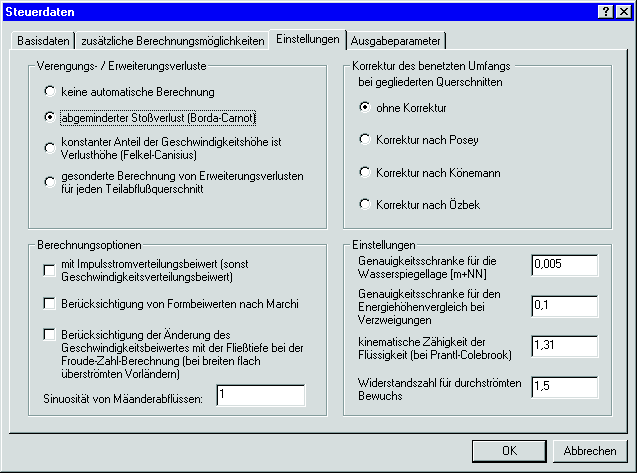
\includegraphics[width=1.0\textwidth]{Einstellungen}
   \caption{Registerkarte \dialog{Einstellungen} in der Dialogmaske \dialog{Steuerdaten}}
   \label{Fortgeschrittene Abb Einstellungen}
\end{figure}

\subsubsection{Verengungs-/Erweiterungsverluste}
Bez\"{u}glich der Ber\"{u}cksichtigung von Verengungs-/Erweiterungsverlusten stehen im Programm vier verschiedene M\"{o}glichkeiten
zur Verf\"{u}gung (vgl. auch Abschnitt~\ref{Fortgeschrittene Subsec Einzelverluste}):
\begin{description}
   \item[Keine automatische Berechnung:] Alle positiv in die Verlustdatei eingegebenen Werte werden als
      Verlustbeiwerte $\zeta$ im Sinne von Gleichung~\ref{Fortgeschrittene Gl Einzelverluste} interpretiert.
   \item[Abgeminderter Sto{\ss}verlust (\autor{Borda-Carnot}):] Die \"{o}rtlichen Verluste werden in Ab\-h\"{a}n\-gigkeit von der
      Geschwindigkeitsh\"{o}hendifferenz $dh_k$ folgenderma{\ss}en berechnet:
      \begin{description}
         \item [Erweiterung, $dh_k < 0$:]
            Die Verluste werden nach dem Ansatz von \autor{Borda-Car\-not}
            (Gleichung~\ref{Fortgeschrittene Gl VerlustBordaCarnot}) f\"{u}r eine Querschnittsaufweitung berechnet. Ein
            positiv in die Verlustdatei eingegebener Wert fungiert dabei als Abminderungsfaktor $c_i$ f\"{u}r den Sto{\ss}verlust.
         \item [Verengung, $dh_k \geq 0$:]
            Die Verluste an Stellen, an denen der Querschnitt eingeengt wird, werden nicht ber\"{u}cksichtigt, solange in der
            Verlustdatei an dieser Stelle kein Wert steht. Ein positiver Wert in der Verlustdatei am stromauf gelegenen
            Profil wird vom Programm als Verlustbeiwert $\zeta$ interpretiert und die Verlusth\"{o}he nach
            Gleichung~\ref{Fortgeschrittene Gl Einzelverluste} berechnet.
      \end{description}

      Soll der \"{o}rtliche Verlust \"{u}ber das Fl\"{a}chenverh\"{a}ltnis abgesch\"{a}tzt werden, so mu{\ss} in der Verlustdatei an dieser Stelle ein negativer Wert stehen. Der Betrag dieses Wertes wird dann als Abminderungsfaktor $c_i$ im Sinne von Gleichung~\ref{Fortgeschrittene Gl Verengungsverluste} gedeutet.

   \item [Konstanter Anteil der Geschwindigkeitsh\"{o}he ist Verlusth\"{o}he (\autor{Felkel-Canisius}):]
         Im Programm WSPLWA wird in Anlehnung an \cite{FelkelCanisius} die
         Geschwindigkeitsverteilung bei der Berechnung der Geschwindigkeitsh\"{o}he ber\"{u}cksichtigt. Der
         Geschwindigkeitsverteilungsbeiwert $\alpha$ wird n\"{a}herungsweise entsprechend Gleichung~\ref{Einstieg Gl
         Geschwindigkeitsverteilung} aus den mittleren Geschwindigkeiten im Flu{\ss}bett und den Vorl\"{a}ndern berechnet, wobei
         die Geschwindigkeitsverteilung in den Teilstromr\"{o}hren selbst durch Ansatz von $\alpha_j = 1$ vernachl\"{a}ssigt wird.
         Der kinetische Energieanteil bzw. die Geschwindigkeitsh\"{o}he wird damit n\"{a}herungsweise aus
         \begin{equation}
            h_k = \frac{\sum \left( v_j^3 \cdot A_j \right)}{2g \cdot Q}
         \end{equation}
         berechnet. Bei Wahl des Ansatzes nach \autor{Felkel-Canisius} wird bei geringeren Flie{\ss}geschwindigkeiten
         ein konstanter Anteil der Geschwindigkeitsh\"{o}hendifferenz als Verlusth\"{o}he angenommen. %Dieser betr\"{a}gt:
%         \begin{equation}
%            H_{ZV} = 2/3 \cdot h_k
%         \end{equation}
         Nimmt die Flie{\ss}geschwindigkeit im Unterwasser zu, so errechnen sich die Verluste im jeweiligen Profil mit Hilfe der
         in der Verlustdatei angegeben Werte nach Gleichung~\ref{Fortgeschrittene Gl Einzelverluste}.
   \item [Gesonderte Berechnung von Erweiterungsverlusten f\"{u}r jeden Teilabflu{\ss}querschnitt:] Bei der gesonderten Berechnung
         der Erweiterungsverluste nach~\cite{KnaufKoennemann} werden f\"{u}r jeden Teilabflu{\ss}querschnitt die Verlusth\"{o}hen mit
         Hilfe der mittleren lokalen Geschwindigkeit im Teilabflu{\ss}querschnitt ermittelt.
\end{description}

\begin{hinweis}
Da die Interpretation der Werte aus der Verlustdatei sowohl von den eingestellten Berechnungsoptionen, als 	auch von den berechneten Geschwindigkeitsh�hen ab\-h�n\-gig ist, sollte immer zun�chst ein erster Berechnungslauf ohne Angabe zu\-s�tz\-li\-cher �rtlicher Verluste mit den voreingestellten Optionen erfolgen.Auf der Grundlage der so erhaltenen Geschwindigkeitsh�hen k�nnen dann gezielt Verlustbeiwerte in die Verlustdatei eingegeben werden.
\end{hinweis}

\subsubsection{Froudezahlberechnung}
Bei praktischen Anwendungen des Rechenprogrammes hat sich gezeigt, da{\ss} die aus
\begin{equation}
   \frac{d H_E}{d h} = \frac{d(W + v_m^2/2g)}{dh}
\end{equation}
mit der N\"{a}herung $\alpha=\mathrm{konstant}$ abgeleitete Gleichung~\ref{Einstieg Gl Froudezahl} f\"{u}r die \autor{Froude}-Zahl
bei sehr breiten Vorl\"{a}ndern und kleinen Flie{\ss}tiefen unrealistisch hohe Werte liefert. Die \"{A}nderung des
Geschwindigkeitsh\"{o}henbeiwertes mit der Flie{\ss}tiefe kann nicht mehr vernachl\"{a}ssigt werden, wenn sich die Abflu{\ss}verteilung im
Flie{\ss}querschnitt mit der Flie{\ss}tiefe sehr stark \"{a}ndert. Dies ist bei breiten, nur flach \"{u}berstr\"{o}mten Vorl\"{a}ndern der Fall.
Ber\"{u}cksichtigt man den Einflu{\ss} der Flie{\ss}tiefenabh\"{a}ngigkeit von $\alpha$, so kommt man nach~\cite{KnaufKoennemann} zu
folgender Absch\"{a}tzung f\"{u}r die \autor{Froude}-Zahl:
\begin{equation}
   \label{Fortgeschrittene Gl Froudezahl}
   Fr = Q \cdot \sqrt{\frac{3 \cdot Z_E \cdot N_E' - N_E \cdot Z_E'}{N_E^4 \cdot 2g}}
\end{equation}
\begin{eqnarray*}
   \textrm{mit} \quad Z_E &=& A_L \cdot v_L^3 + A_F \cdot v_F^3 + A_R \cdot v_R^3 \\
                      Z_E'&=& c_E \cdot (b_L \cdot v_L^3 + b_F \cdot v_F^3 + b_R \cdot v_R^3) \\
                      N_E &=& v_L \cdot A_L + v_F \cdot A_F + v_R \cdot A_R \\
                      N_E'&=& c_N \cdot (v_L \cdot b_L + v_F \cdot b_F + v_R \cdot b_R)
\end{eqnarray*}
\begin{quote}
   Entsprechend dem jeweiligen Flie{\ss}gesetz sind f\"{u}r die Ableitungskonstanten $c_E$ und $c_N$ folgende Werte einzusetzen:
   \begin{quote}
      \begin{tabular}{lcc}
         \autor{Manning-Strickler}  &  $\quad c_E = 3,0$   &  $\quad c_N = 1,66$  \\
         \autor{Prandtl-Colebrook}  &  $\quad c_E = 2,5$   &  $\quad c_N = 1,50$
      \end{tabular}
   \end{quote}
\end{quote}
Eine generelle Anwendung von Gleichung~\ref{Fortgeschrittene Gl Froudezahl} zur Berechnung der \autor{Froude}-Zahl ist
m\"{o}g\-lich. Da in der Praxis bisher meist nur Gleichung~\ref{Einstieg Gl Froudezahl} verwendet wird, wird die aufwendigere
Gleichung~\ref{Fortgeschrittene Gl Froudezahl} im Rechenprogramm nur bei Eingabe eines entsprechenden Steuerparameters
\checkbox{Ber\"{u}cksichtigung der \"{A}nderung des Geschwindigkeitsbeiwertes mit der Flie{\ss}tiefe bei der Froude-Zahl-Berechnung}
verwendet. Die \autor{Froude}-Zahl geht nicht direkt in die Berechnung der Wasserspiegellagen ein, sie dient lediglich zur
Ermittlung und Kennzeichnung des Flie{\ss}zustandes.


\subsubsection{Zusatzparameter}
Unter der Registerkarte \dialog{Einstellungen}, k\"{o}nnen verschiedene f\"{u}r die Berechnung relevante Parameter, die
standardm\"{a}{\ss}ig vorbesetzt sind, editiert werden. Eine \"{A}nderung der voreingestellten Werte ist im allgemeinen nicht
erforderlich.
\begin{description}
   \item[Genauigkeitsschranke f\"{u}r die Wasserspiegellage:] ~\newline
      Die Genauigkeitsschranke f\"{u}r die Wasserspiegellagenberechnung ist im Programm auf
      \mbox{$\mathit{EPSH} = 0,005\unit{m}$} voreingestellt.
   \item[Genauigkeitsschranke f\"{u}r den Energieh\"{o}henvergleich bei Verzweigungen:] ~\newline
      Der Ab\-bruch der iterativen Berechnungen an Verzweigungen erfolgt bei Unterschreitung der Genauigkeitsschranke
      $\mathit{EPSV}$f\"{u}r den Energieh\"{o}henvergleich an der Verzweigungsstelle. Diese ist auf $0,10\unit{m}$ voreingestellt.
%      Die Ge\-nauig\-keitsschranke f\"{u}r den Abbruch der iterativen Berechnung bei Verzweigungen ist mit \mbox{$\mathit{EPSV} =
%      0,01\unit{m}$} vorbelegt.
   \item[kinematische Z\"{a}higkeit der Fl\"{u}ssigkeit:] ~\newline
      Die kinematische Z\"{a}higkeit einer Fl\"{u}ssigkeit ist von der Temperatur der Fl\"{u}ssigkeit abh\"{a}ngig. Voreingestellt ist die
      kinematischen Z\"{a}higkeit von Wasser bei einer Temperatur von 10\grad C:
      \begin{equation*}
         \nu = 1,31 \cdot 10^{-6}\unit{m^2/s}
      \end{equation*}
      Der Wert der kinematische Z\"{a}higkeit wird programmintern mit $10^{-6}$ multipliziert.
   \item[Widerstandszahl f\"{u}r durchstr\"{o}mten Bewuchs:] ~\newline
      In der Standardeinstellung betr\"{a}gt die Widerstandszahl f\"{u}r
      durchstr\"{o}mten Bewuchs $c_{WR} = 1,5$. Der Zahlenbereich f\"{u}r die Eingabe ist auf $1.0 < c_{WR} < 1.6$ eingeschr\"{a}nkt.
\end{description}

\subsubsection{Sinuosit\"{a}t}
\autor{Chow}~\cite{Chow} empfiehlt den \autor{Manning-Strickler}-Beiwert bei M\"{a}andrierung eines Gew\"{a}s\-sers zu erh\"{o}hen.
Kennzeichnende Gr\"{o}{\ss}e ist hierbei die Sinousit\"{a}t $S_M$ eines M\"{a}anders:
\begin{eqnarray*}
   \begin{minipage}{0.40\textwidth}
      \hspace{0.5cm}
      
\includegraphics{Maeander}
   \end{minipage}
   \begin{minipage}{0.6\textwidth}
      \begin{equation}
         S_M = \frac{\textrm{Talweg des M"aanders}}{\textrm{Wellenl"ange des M"aanders}}
      \end{equation}
      \\ \\
   \end{minipage}
\end{eqnarray*}
Nach~\cite{BWK1999} kann die Empfehlung von~\autor{Chow} in einen Korrekturfaktor zum Widerstandsbeiwert $\lambda$ bei
Kompaktquerschnitten wie folgt umgesetzt werden:
\begin{equation}
   \lambda_{ges,M} = c_{M,K} \cdot \lambda_{ges}
\end{equation}
\begin{quote}
   \textrm{mit} \qquad
   \begin{tabular}{lll}
      $c_{M,K} = 6,40 \cdot S_M - 5,40$   &  f\"{u}r   &  $1,00 < S_M \leq 1,05$ \\
      $c_{M,K} = 0,822 \cdot S_M + 0,45$  &  f\"{u}r   &  $1,05 < S_M \leq 1,50$ \\
      $c_{M,K} = 1,69$                    &  f\"{u}r   &  $1,50 < S_M$
   \end{tabular}
\end{quote}
Bei gegliederten Querschnitten erh\"{o}ht sich der Korrekturfaktor nach~\cite{BWK1999} entsprechend
\begin{equation}
   c_{M,G} = 1,0 + (2,5 \cdot c_{M,K} - 1,0)
\end{equation}
Die Verwendung von pauschalen Faktoren zur Erh\"{o}hung der Reibungsbeiwerte k\"{o}nnen dem tats\"{a}chlichen Einflu{\ss} einer
M\"{a}andrierung nur n\"{a}herungsweise Rechnung tragen. Bei starker M\"{a}andrierung oder besonderen Genauigkeitsanforderungen ist
der Anwendungsbereich einer eindimensionalen Str\"{o}mungsberechnung nicht mehr gegeben.

\subsubsection{Formbeiwert nach Marchi}
Das Widerstandsgesetz von \autor{Prandtl-Colebrook} wurde f\"{u}r Rohrstr\"{o}mungen mit \"{u}ber den benetzten Umfang gleichm\"{a}{\ss}ig
verteilten Wandschubspannungen entwickelt. Bei Gerinnestr\"{o}mungen mit freiem Wasserspiegel ist diese Voraussetzung nicht
gegeben.

Bei Kompaktquerschnitten entstehen Sekund\"{a}rstr\"{o}mungen, die eine ungleichm\"{a}{\ss}ige Geschwindigkeitsverteilung und eine
ungleichm\"{a}{\ss}ige Wandschubspannungsverteilung verursachen. Zum Ausgleich dieser Abweichungen ist das einparametrige
Formbeiwertkonzept von \autor{Marchi} \cite{SchroederRCM2} bei einer eindimensionalen Str\"{o}mungsberechnung zu empfehlen.
Bei diesem Konzept wird mit einer Korrektur des f\"{u}r die Wandschubspannung repr\"{a}sentierenden hydraulischen Radius
gearbeitet:
\begin{equation}
   d_{\mathit{eff}} = f \cdot d = f \cdot 4 \cdot r_{hy}
\end{equation}
Diese Korrektur ver\"{a}ndert die Konstanten der \autor{Prandtl-Colebrook}-Formel:
\begin{equation*}
   C_1 = 2,51 / f    \quad  \textrm{und}  \quad C_2 = 3,71 \cdot f
\end{equation*}

Nat\"{u}rliche Flie{\ss}querschnitte k\"{o}nnen am einfachsten durch hydraulisch gleichwertige Rechteckquerschnitte angen\"{a}hert werden.
F\"{u}r rechteckige Querschnitte ergibt sich ein Formbeiwert zwischen $f = 0,52$ (sehr breite Querschnitte $h/b \Rightarrow
0$) und $f = 0,9$ (Quadrat). Durch die Formbeiwerte ver\"{a}ndern sich die Zahlenwerte der Prandtl-Colebrook-Formel wie in
Tabelle~\ref{Fortgeschrittene Tab FormbeiwertMarchi} angegeben.

\begin{table}[hbt]
   \centering
   \input{Fortgeschrittene/tab/FormbeiwertMarchi.tab}
   \caption{Formbeiwerte nach Marchi}
   \label{Fortgeschrittene Tab FormbeiwertMarchi}
\end{table}

Als Bestimmungsgleichung f\"{u}r den Formbeiwert beliebiger Rechtecke ist in \cite{SchroederRCM2} folgende Sch\"{a}tzformel
angegeben:
\begin{equation}
   f = 0,09 - 0,38 \cdot e^{-5h/b}
\end{equation}
F\"{u}r teilgef\"{u}llte Kreisquerschnitte hat \autor{Bock} Formbeiwerte zwischen 0,4 und 1,0 gemessen. Eine polynomische
Anpassung der Me{\ss}werte f\"{u}hrt auf folgende Bestimmungsgleichung f\"{u}r Formbeiwerte beim teilgef\"{u}llten Kreisquerschnitt:
\begin{equation}
   f = 0,3458 + 2,2026 \cdot \frac{h}{d} - 2,4566 \cdot \left( \frac{h}{d} \right)^2
       + 0,9084 \cdot \left( \frac{h}{d} \right)^3
\end{equation}

\subsubsection{Korrektur des benetzten Umfangs}
Eine ungleichm\"{a}{\ss}ige Geschwindigkeitsverteilung in einem Flie{\ss}querschnitt vermindert die hydraulische Leistungsf\"{a}higkeit,
da das Reibungsgef\"{a}lle linear mit dem Geschwindigkeitsverteilungsbeiwert zunimmt. Bei gegliederten Querschnitten
vergr\"{o}{\ss}ert sich das Energieliniengef\"{a}lle weiterhin durch zus\"{a}tzliche Interaktionswiderst\"{a}nde an den Trennfl\"{a}chen zwischen
den Vorl\"{a}ndern mit kleiner Flie{\ss}geschwindigkeit und dem Flu{\ss}schlauch mit gr\"{o}{\ss}erer Flie{\ss}geschwindigkeit.

Zum Ausgleich dieser zus\"{a}tzlichen Flie{\ss}widerst\"{a}nde wird in der Fachliteratur eine Vergr\"{o}{\ss}erung des benetzten Umfanges im
Flu{\ss}schlauch unter Beibehaltung der hydraulischen Radien im Vorland empfohlen. Nach Untersuchungen von
\autor{Kradolfer}~\cite{Kradolfer} und \autor{Knauf}~\cite{Knauf1} kann diese Korrektur zu unsinnigen Ergebnissen f\"{u}hren,
wenn sie ohne Beachtung der zul\"{a}ssigen Anwendungsgrenzen angewendet wird. Im Programmsystem stehen drei verschiedene
Korrekturm\"{o}glichkeiten zur Verf\"{u}gung:
\begin{description}
   \item[Korrektur nach Posey:] Nach Untersuchungen von \autor{Posey} im Jahre 1967 \cite{Kradolfer} nimmt der
      Korrekturbedarf mit zunehmender Flie{\ss}tiefe im Vorland ab. Bei Verh\"{a}ltnissen \mbox{$h_V > 0,5 h_F$} sollten auch
      gegliederte Flie{\ss}querschnitte ohne Bewuchs wie Kompaktquerschnitte berechnet werden \cite{Knauf1, ATV111}.
      Der abnehmende Einflu{\ss} des Zusatzwiderstandes kann entsprechend~\cite{ATV111} durch folgende Korrekturgr\"{o}{\ss}e zum
      benetzten Umfang des Flu{\ss}schlauchs n\"{a}herungsweise automatisch ber\"{u}cksichtigt werden:
      \begin{equation}
         \begin{split}
            U_{F,cal} &= U_F + U_{T,L} + U_{T,R} \\
            U_{F,cal} &= U_F + h_{V,L} \cdot \left( 1 - \frac{2h_{V,L}}{h_F} \right)
                         + h_{V,R} \cdot \left( 1 - \frac{2h_{V,R}}{h_F} \right)
         \end{split}
      \end{equation}
   \item[Korrektur nach K\"{o}nemann:]
      Meist wird die von \autor{K\"{o}nemann} vorgeschlagene Korrektur empfohlen~\cite{SchroederW, DVWK1991}, ohne auf die
      Anwendungsgrenzen besonders hinzuweisen. Die Korrektur besteht in der Vergr\"{o}{\ss}erung des benetzten
      Flu{\ss}schlauch-Umfanges durch die vollen Trennfl\"{a}chenh\"{o}hen, wobei die Trennfl\"{a}chenrauheit selbst in erster N\"{a}herung
      gleich der angrenzenden Wandfl\"{a}chenrauheit des Flu{\ss}schlauchs gesetzt wird.
      \begin{equation}
         U_{F,cal} = U_F + U_{T,L} + U_{T,R}  \qquad   \textrm{mit}   \qquad   k_T = k_W
      \end{equation}
      Diese Korrektur ist nur f\"{u}r kleine Vorlandflie{\ss}tiefen \mbox{$h_V < h_F/3$} zu empfehlen und nur bei gegliederten
      Gerinnen \emph{ohne} Bewuchs anwendbar.
   \item[Korrektur nach \"{O}zbek:]
      Bei kleinen Flie{\ss}tiefen im Vorland \mbox{($h_V < h_F/3$)} wird in~\cite{DVWK1991} ein Sicherheitsfaktor von mind. 3
      zur Vergr\"{o}{\ss}erung der Trennfl\"{a}chenrauheit empfohlen. Zur Verbesserung dieser unbefriedigenden Situation haben
      \autor{Bretschneider} und \autor{\"{O}zbek} (1997) anhand von Modellversuchen (SERC, Wallingford, UK) eine Sch\"{a}tzformel
      zur Ermittlung der Trennfl\"{a}chenrauheit $\lambda_T$ bei kleinen Vorland\-\"{u}berstr\"{o}mungen abgeleitet :
      \begin{equation}
         \lambda_T = 0,71 \cdot \left(\frac{b_V}{b_F} \right)^{0,48}
                     \cdot \left(\frac{h_F}{h_V} \right)^{1,05} \cdot \lambda_W
      \end{equation}
      Entsprechend den Modellversuchen werden die G\"{u}ltigkeitsgrenzen wie folgt angegeben:
      \begin{quote}
         Tiefenverh\"{a}ltnis:    \quad    $h_F/h_V > 2$, \\
         Breitenverh\"{a}ltnis:   \quad    $b_V/b_F \leq 4,56$
      \end{quote}
      Diese Korrektur ist nur bei gegliederten Gerinnen und einer Berechnung mit dem Flie{\ss}gesetz von
      \autor{Prandtl-Colebrook} \emph{ohne} Bewuchs anwendbar.
\end{description}


\subsubsection{Impulsstromverteilungsbeiwert}
In~\cite{BWK1999} wird empfohlen bei konstanten Abfl\"{u}ssen die ma{\ss}gebende Energieh\"{o}he mit Hilfe des
Geschwindigkeitsverteilungsbeiwertes zu ermitteln und bei diskontinuierlichen Abfl\"{u}ssen den Impulsstromverteilungsbeiwert
zu verwenden. Die Berechnung der ma{\ss}gebenden Energieh\"{o}he kann von \wspwin{} wahlweise mit dem
Geschwindigkeitsverteilungsbeiwert $\alpha$ nach Gleichung~\ref{Einstieg Gl Geschwindigkeitsverteilung}
(Standardeinstellung) oder, falls das entsprechende Kontrollk\"{a}stchen bet\"{a}tigt wurde, mit dem Impulsstromverteilungsbeiwert
$\alpha'$ nach Gleichung~\ref{Einstieg Gl Impulsstromverteilung} berechnet werden.

\clearpage
\subsection{Ausgabeparameter}

\begin{figure}[hbt]
   \centering
   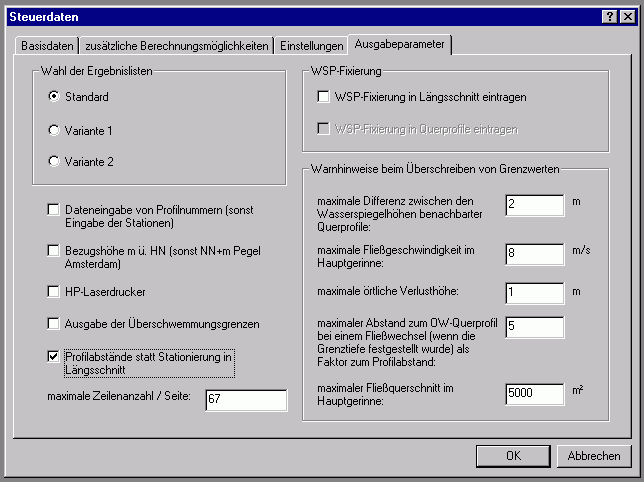
\includegraphics[width=1.0\textwidth]{Ausgabeparameter}
   \caption{Registerkarte \dialog{Ausgabeparameter} in der Dialogmaske \dialog{Steuerdaten}}
   \label{Fortgeschrittene Abb Ausgabeparameter}
\end{figure}


\subsubsection{Wahl der Ergebnislisten}
Bez\"{u}glich des Darstellungformates der Ergebnisdateien kann zwischen drei unterschiedlichen Ausgabevarianten gew\"{a}hlt
werden. Die Ausgabe der einzelnen hydraulischen Parameter, Wasserspiegellagen etc. erfolgt in Form einer Tabelle. Wenn Sie
die Voreinstellung nicht \"{a}ndern, wird das Standardformat (Abbildung~\ref{Fortgeschrittene Abb Standardausgabe}) f\"{u}r die
Ausgabe verwendet.

Die Ausgabe der Variante~1 (vgl. Abbildung~\ref{Fortgeschrittene Abb AusgabeVariante1}) enth\"{a}lt zus\"{a}tzlich zu den
Parametern der Standardausgabe die berechneten Schleppspannungen auf den Vorl\"{a}ndern und im Flu{\ss}schlauch sowie die
Verlustbeiwerte $\zeta$. Daf\"{u}r sind Geschwindigkeits-, Impulsstromverteilungsbeiwerte und Flie{\ss}fl\"{a}chen nicht in der
Ergebnisdarstellung enthalten.

Variante~2 (vgl. Abbildung~\ref{Fortgeschrittene Abb AusgabeVariante2}) stellt die Ergebnisse der Berechnung in zwei
Tabellen untereinander dar. Die erste Tabelle gibt dabei nur die Wasserspiegellage und die Energieh\"{o}he an der Station
wieder. In der zweiten Tabelle sind die hydraulischen Parameter zusammengefa{\ss}t.

%Sollten Sie \"{u}ber einen HP-Laserdrucker verf\"{u}gen, kann es vorteilhaft sein, die Zusatzoption \checkbox{HP-Laserdrucker}
%aktivieren.

\begin{sidewaysfigure}[hbt]
   \centering
   \input{Fortgeschrittene/tab/Standardausgabe.tab}
   \caption{Ergebnisdarstellung bei der Standardausgabe}
   \label{Fortgeschrittene Abb Standardausgabe}
\end{sidewaysfigure}
\begin{sidewaysfigure}[hbt]
   \centering
   \input{Fortgeschrittene/tab/AusgabeVariante1.tab}
   \caption{Ergebnisdarstellung der Variante~1}
   \label{Fortgeschrittene Abb AusgabeVariante1}
\end{sidewaysfigure}
\begin{sidewaysfigure}[hbt]
   \centering
   \input{Fortgeschrittene/tab/AusgabeVariante2.tab}
   \caption{Ergebnisdarstellung der Variante~2}
   \label{Fortgeschrittene Abb AusgabeVariante2}
\end{sidewaysfigure}

\clearpage
\subsubsection{Profilnummern}
Anstelle der Stationierung konnten in der ehemaligen DOS-Version die Profilnummern ausgedruckt werden. Es war dann die
entsprechende Option einzugeben, die in der Windows-Version keine Bedeutung mehr besitzt.

\subsubsection{Bezugsh\"{o}he}
Als Bezugsh\"{o}he f\"{u}r den tabellarischen Ergebnisausdruck kann wahlweise der Pegel Amsterdam  oder der Pegel Kronstadt
gew\"{a}hlt werden. In letzterem Fall ist das K\"{a}stchen \checkbox{Bezugsh\"{o}he m \"{u}. HN} auf der Registerkarte
\dialog{Ausgabeparameter} zu markieren.
\begin{quote}
   \begin{tabular}{lll}
      \textbf{Pegel}    &  \textbf{H\"{o}henangabe} \\[3pt]
      Amsterdam: \qquad  &  NN+m \\
      Kronstadt:        &  m \"{u} HN
   \end{tabular}
\end{quote}
Die Berechnung ist nicht an die Wahl eines der beiden H\"{o}henbezugssysteme gebunden. Sie k\"{o}nnen bei der Eingabe der Daten
jede beliebige Referenzh\"{o}he verwenden. Die Einheiten sind dann ggf. im Ergebnisausdruck von Hand anzupassen.


\subsubsection{Ausgabe von \"{U}berschwemmungsgrenzen}
%Scheint nicht zu funktionieren.
Durch Aktivieren der Option \checkbox{Ausgabe der \"{U}berschwemmungsgrenzen} werden diese in einer eigenen Datei im
Projektunterverzeichnis \datei{...\textbackslash dath} ihres aktuelles Projektes gepeichert. Der vierte und f\"{u}nfte
Buchstabe des Dateinamens lautet \datei{*ug*.*}, beispielsweise enth\"{a}lt die Datei \datei{fuug0001.001} die
\"{U}berschwemmungsgrenzen einer Berechnung an der Fulda.

\subsubsection{HP-Laserdrucker}
Verwenden Sie einen HP-Laserdrucker zur Ausgabe der Berechnungsergebnisse, so kann es von Vorteil sein, wenn diese Option
markiert wird.

\subsubsection{Zeilenanzahl}
\"{U}ber ein Editierfeld kann die vorgegebene Zeilenanzahl im Resultatausdruck ge\"{a}ndert werden. Standardm\"{a}{\ss}ig werden in der
Ergebnisdatei 67~Zeilen/Seite dargestellt. Sollten Sie mehr oder weniger Zeilen darstellen m\"{o}chten, k\"{o}nnen Sie die
entsprechende \"{A}nderung hier vornehmen.


\subsubsection{Wasserspiegelfixierungen}
Unter dem Men\"{u}punkt Zustand (vgl. Abschnitt~\ref{Einstieg Subsec Abflussdatei}) haben Sie die M\"{o}glichkeit, f\"{u}r einzelne
Abflu{\ss}ereignisse gemessene Wasserspiegellagen an den jeweiligen Stationen einzutragen. Wenn Sie m\"{o}chten, da{\ss} diese
Wasserspiegelfixierungen im Rahmen der Berechnung automatisch in die Querprofile und L\"{a}ngsschnitte mit eingetragen werden,
so markieren Sie \checkbox{WSP-Fixierung in L\"{a}ngsschnitt eintragen}. Der Eintrag in die Querprofile kann erst vorgenommen
werden, wenn der Eintrag in den L\"{a}ngsschnitt aktiviert ist.

\clearpage
\subsubsection{Warnhinweise beim \"{U}berschreiten von Grenzwerten}
\wspwin{} gibt bei der \"{U}berschreitung von Grenzwerten Warnungen im Ergebnisausdruck aus. Im Fall der Standardeinstellungen
erfolgt eine Warnung, wenn
\begin{itemize}
   \item die Differenz der Wasserspiegelh\"{o}hen in benachbarten Querprofilen $2,0\unit{m}$ \"{u}berschreitet,
   \item die maximale Flie{\ss}geschwindigkeit im Hauptgerinne gr\"{o}{\ss}er als $8,0\unit{m/s}$ ist,
   \item die \"{o}rtliche Verlusth\"{o}he den Wert von $1,0\unit{m}$ erreicht,
   \item der Abstand des oberwasserseitigen Querprofils bei einem Flie{\ss}wechsel gr\"{o}{\ss}er als der f\"{u}nffache Profilabstand wird,
   \item der Flie{\ss}querschnitt die Grenze von $5000\unit{m^2}$ \"{u}berschreitet.
\end{itemize}


\subsection{Massenberechnung}

\wspwin{} kann mit einem Zusatzmodul zur Massenberechnung geliefert werden. Berechnet werden im einzelnen:
\begin{itemize}
   \item Auf- und Abtragsfl\"{a}che sowie die daraus resultierende Fl\"{a}chendifferenz f\"{u}r alle Stationen, differenziert nach
       linkem/rechtem Vorland und Hauptgerinne. Die Differenzierung in Vorl\"{a}nder und Flu{\ss}schlauch erfolgt anhand der
       Trennfl\"{a}chen bzw. B\"{o}schungsoberkanten des Referenzzustandes.
   \item Massenberechnung f\"{u}r einzelne Berechnungsabschnitte unterteilt f\"{u}r Vorl\"{a}nder und Flu{\ss}schlauch. Positive Werte
      kennzeichnen Auf-, negative Abtrag. Das Volumen ergibt sich aus Multiplikation der Fl\"{a}chendifferenz mit der L\"{a}nge des
      Berechnungsabschnitts.
      \begin{equation}
         \begin{minipage}{0.45\linewidth}
            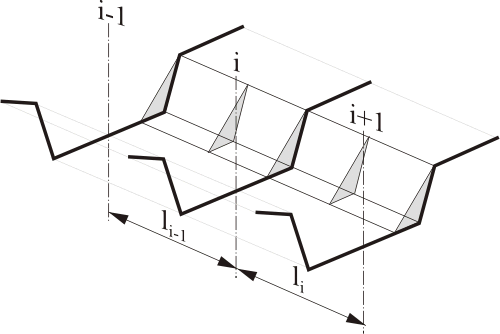
\includegraphics[width=1.0\linewidth]{Massenberechnung}
         \end{minipage}
         \qquad \Delta V_i = \Delta A_i \cdot \frac{l_{i-1} + l_i}{2}
      \end{equation}
   \item Masse der Einzelabschnitte
   \item resultierende Gesamtmasse
\end{itemize}
Voraussetzungen f\"{u}r die Durchf\"{u}hrung einer Massenberechnung zwischen zwei Zust\"{a}n\-den sind der gleiche Gew\"{a}ssername im
Referenz- und Vergleichszustand und Profile mit gleichen Stationsangaben sowie identischen Gel\"{a}ndekoordinaten am jeweils
ersten und letzten Profilpunkt. Parallel zur Massenberechnung kann auch  eine Gel\"{a}ndeverkn\"{u}pfung bzw. Fl\"{a}chenberechnung
nach Abschnitt~\ref{Fortgeschrittene Subsec Vergleichszustaende} durchgef\"{u}hrt werden. Dies erm\"{o}glicht es, die Gel\"{a}ndeh\"{o}hen
der einzelnen Profile im Referenz- und Vergleichszustand direkt (auch optisch) zu vergleichen.
\begin{sidewaysfigure}[hbt]
   \centering
   \input{Fortgeschrittene/tab/Massenberechnung.tab}
   \caption{Ergebnis der Massenberechnung}
   \label{Fortgeschrittene Abb Massenberechnung}
\end{sidewaysfigure}

Um den Massenunterschied zwischen zwei unterschiedlichen Ausbauzust\"{a}nden eines Gew\"{a}ssers zu ermitteln, w\"{a}hlen Sie die
Men\"{u}folge \menu{\marrow \underline{B}erechnung \marrow \underline{M}assenberechnung}. Sie m\"{u}ssen nun zun\"{a}chst den
Referenzzustand und den Vergleichszustand ausw\"{a}hlen. Danach wird die Massenberechnung gestartet. Die Ergebnisse werden in
im Unterverzeichnis \datei{...\textbackslash dath} Ihres Projektverzeichnisses unter dem Dateinamen \datei{masse.txt}
abgelegt. Dabei wird eine bereits bestehende Ergebnisdatei \"{u}berschrieben. Die Datei kann im Editor eingesehen werden. Der
Aufruf erfolgt \"{u}ber das Men\"{u} \menu{\marrow \underline{E}rgebnisse \marrow Ergebnisse der \underline{M}assenberech\-nung}.
\begin{hinweis}
   M\"{o}chten sie die Ergebnisse einer fr\"{u}heren Massenberechnung im gleichen Projekt nicht \"{u}berschreiben, so speichern sie
   die Datei \datei{masse.txt} vor einer erneuten Berechnung unter einem anderen Namen.
\end{hinweis}


\subsection{Sonderprogramme station\"{a}r gleichf\"{o}rmig}

Aus \wspwin{} heraus k\"{o}nnen Sonderprogramme des Programmsystems HYDRA u.a. zu station\"{a}r gleichf\"{o}rmigen Berechnungen
aufgerufen werden. Es handelt sich hierbei um DOS-Programme, die in einem DOS-Fenster ablaufen. Folgende Programme sind
(sofern erworben) verf\"{u}gbar:
\begin{itemize}
   \item Wehre
   \item Rohre
   \item Gerinne
   \item Stra{\ss}enbau
   \item Entlastungsbauwerke
\end{itemize}
Weitere Angaben hierzu finden Sie im Kapitel~\ref{Dialogprogramme}.




\clearpage
%%%%%%%%%%%%%%%%%%%%%%%%%%%%%%%%%%%%%%%%%%%%%%%%%%%%%%%%%%%%%%%%%%%%%%%%%%%%%%%%%%%%%%%%%%%%%%%%%%%%%%%%%%%%%%%%%%%%%%%%%%%%
\section{Ergebnisse einsehen}
%%%%%%%%%%%%%%%%%%%%%%%%%%%%%%%%%%%%%%%%%%%%%%%%%%%%%%%%%%%%%%%%%%%%%%%%%%%%%%%%%%%%%%%%%%%%%%%%%%%%%%%%%%%%%%%%%%%%%%%%%%%%

Im Rahmen der Bearbeitung mit \wspwin{} werden die nachfolgend aufgef\"{u}hrten Ergebnisdateien im Projektunterverzeichnis
\datei{...\textbackslash dath} erstellt. Der Dateiname leitet sich im allgemeinen aus dem Namen der zugrunde gelegten
Berechnungsvariante ab, wobei lediglich die dritten und vierten Buchstaben modifiziert werden. F\"{u}r eine
Berechnungsvariante an der Fulda \datei{fu000001.001} erg\"{a}ben sich folgende Ergebnisdateien: \\ ~ \\

\input{Fortgeschrittene/tab/Ergebnisdateien.tab}


\subsection{L\"{a}ngsschnitte einsehen und vergleichen}

Nach der Berechnung k\"{o}nnen die Ergebnisse in einer L\"{a}ngsschnittgrafik eingesehen werden (Abschnitt~\ref{Einstieg Subsec
Laengsschnitteditor}). Die Darstellung l\"{a}{\ss}t sich bearbeiten. So macht es beispielsweise Sinn, bei verzweigten Systemen
einzelne Profilpunkte zu l\"{o}schen, um eine eindeutige Darstellung zu erhalten. Sie entfernen nicht mehr ben\"{o}tigte Stationen
aus der Grafik, indem sie die zugeh\"{o}rigen $y$-Werte l\"{o}schen. Sowohl die Profildatei als auch die Grafik werden dann
aktualisiert.

Die Datens\"{a}tze \afz{Text} und \afz{Bauwerk} k\"{o}nnen nicht \"{u}ber \wspwin{} editiert werden. Das L\"{o}schen der kompletten
Datens\"{a}tze ist allerdings m\"{o}glich. Diese Datenblocktypen sind lediglich f\"{u}r das sp\"{a}tere Plotten relevant.

Beim Einsehen des L\"{a}ngsschnitts besteht ferner die M\"{o}glichkeit, verschiedene Berechnungsvarianten zu vergleichen. W\"{a}hlen
Sie hierzu aus dem L\"{a}ngsschnitteditor heraus die Men\"{u}folge \menu{ \marrow Ergebnisse \marrow L\"{a}ngsschnitt vergleichen}.
Sie werden dazu aufgefordert, eine weitere Berechnungsvariante auszuw\"{a}hlen. Sobald Sie eine Variante ausgew\"{a}hlt haben,
werden aus dieser Datei die Datens\"{a}tze \afz{Sohlh\"{o}he}, \afz{B\"{o}schung li.} , \afz{B\"{o}schung re.} und der \afz{Wasserspiegel}
als \afz{2.~Sohlh\"{o}he}, \afz{2.~Wasserspiegel} etc. in ihre aktuelle L\"{a}ngsschnittdatei eingef\"{u}gt.

Bei jedem Aufruf des L\"{a}ngsschnitteditors erscheint die Meldung \afz{Es existiert bereits eine L\"{a}ngsschnittdatei.
\"{U}berschreiben?}. Ein \"{U}berschreiben der L\"{a}ngsschnittdatei ist dann sinnvoll, wenn Sie die Datei komplett neu aus den
Berechnungsergebnissen erstellen lassen wollen. Haben Sie hingegen bereits in der Datei gespeicherte Stempeldaten und
Plotinformationen eingegeben, so kann die alte L\"{a}ngsschnittdatei erhalten bleiben.


\clearpage
\subsection{Berechnungsergebnisse auswerten}
\wspwin{} verf\"{u}gt \"{u}ber drei Auswerteprogramme, mit denen es m\"{o}glich ist, sich Listen von Auswertungen der
Berechnungsergebnisse erstellen zu lassen.

\subsubsection{Listenauswertung}
Das Modul WSPLIST wertet \"{U}berflutung und Vollf\"{u}llung der Gew\"{a}sser aus. Hierzu mu{\ss} die automatische Berechnung einer
Abflu{\ss}kurve mit fester Schrittweite vorliegen. Die Definition des bordvollen Abflusses orientiert sich dabei an folgenden
Gr\"{o}{\ss}en:
\begin{itemize}
   \item erster und letzter Profilpunkt
   \item Grenzen der durchstr\"{o}mten Bereiche
   \item bei geschlossenen Durchl\"{a}ssen der h\"{o}chste Punkt
   \item bei \"{u}berstr\"{o}mten Durchl\"{a}ssen die \"{U}berstr\"{o}mungsh\"{o}he
   \item bei offenen Profilen die Lage der Trennfl\"{a}chen (hierdurch k\"{o}nnen wahlweise bordvolle Abfl\"{u}sse des Flu{\ss}schlauchs
      oder des Gesamtquerschnitts mit Vorl\"{a}ndern definiert werden)
\end{itemize}
Im Men\"{u} \menu{\marrow \underline{E}rgebnisse} finden Sie das Untermen\"{u} \menu{\marrow Auswer\underline{t}en \marrow
Beispie\underline{l}listen}. Nach dessen Aufruf erscheint zun\"{a}chst der Dialog zur Auswahl von Berechnungsvarianten. Mit
\schalter{Berechnung} wird das Auswerteprogramm gestartet. Nach der Auswertung werden Ihnen automatisch die Ergebnisse im
\wspwin{}-Editor angezeigt. Sie k\"{o}nnen die Ergebnisse auch sp\"{a}ter jederzeit \"{u}ber den Editor einsehen. \newline Folgende
Ergebnisdateien werden erstellt:
\begin{description}
   \item[\datei{*wk*.*}:] Enth\"{a}lt eine Liste aller Profile geordnet nach Abfl\"{u}ssen, mit Wassertiefe und
            Wasserspiegelbreite (Abbildung~\ref{Fortgeschrittene Abb DateiWK}).
   \item[\datei{*ue*.*}:]  Enth\"{a}lt eine Liste aller Abfl\"{u}sse geordnet nach Stationen mit \"{U}berlastungen links und rechts
            (Abbildung~\ref{Fortgeschrittene Abb DateiUE}).
   \item[\datei{*ma*.*}:] Wertet die Ergebnisdateien soweit aus, da{\ss} nur der bordvolle Abflu{\ss} $Q_{voll}$ im Profil in der
      Liste steht (Abbildung~\ref{Fortgeschrittene Abb DateiMA}).
   \item[\datei{*ex*.*}:] Ausgabe von L\"{a}ngsschnittdaten f\"{u}r einen Import in Excel. Die erste Zeile enth\"{a}lt die
      Abflu{\ss}ereignisse, in der ersten Spalte sind die Stationen verzeichnet.
\end{description}
\begin{figure}[hbtp]
   \centering
   \input{Fortgeschrittene/tab/DateiWK.tab}
      \caption{Datei \datei{*wk*.*} des Beispiels \afz{Testbach}}
      \label{Fortgeschrittene Abb DateiWK}
   \input{Fortgeschrittene/tab/DateiUE.tab}
      \caption{Datei \datei{*ue*.*} des Beispiels \afz{Testbach}}
      \label{Fortgeschrittene Abb DateiUE}
   \input{Fortgeschrittene/tab/DateiMA.tab}
      \caption{Datei \datei{*ma*.*} des Beispiels \afz{Testbach}}
      \label{Fortgeschrittene Abb DateiMA}
\end{figure}
Die Ergebnisse werden im Unterverzeichnis \datei{\textbackslash dath} abgelegt. Der Dateiname orientiert sich am Namen der
ersten ausgew\"{a}hlten Berechnungsvariante, deren 3. und 4. Buchstabe variiert.


\subsubsection{Vergleichslisten}
Neben dem Listenprogramm zur Auswertung von \"{U}berflutungen kann ein weiteres Zusatzmodul genutzt werden, das verschiedene
hydraulische Parameter aus bis zu drei Berechnungsvarianten miteinander vergleicht. Der Vergleich wird \"{u}ber das Men\"{u}
\menu{\marrow \underline{E}rgebnis\-se \marrow Auswer\underline{t}en \marrow \underline{V}ergleichen} initialisiert. Die
Auswahl der Berechnungsvarianten erfolgt in gleicher Weise wie beim Listenprogramm. Zus\"{a}tzlich erscheint jedoch ein
weiterer Dialog in dem sie einen oder mehrere zu vergleichenden Parameter ausw\"{a}hlen m\"{u}ssen
(Abbildung~\ref{Fortgeschrittene Abb AuswahlVergeleichswerte}). Die Ausgabe (vgl. Abbildung~\ref{Fortgeschrittene Abb
Vergleichsliste}) enth\"{a}lt neben den einzelnen Parametern an der Station auch die jeweilige Differenz zum Referenzzustand.
\begin{figure}[hbt]
   \centering
   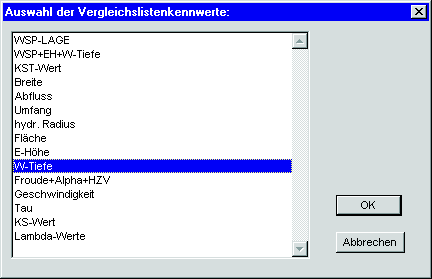
\includegraphics[width=0.8\textwidth]{AuswahlVergleichswerte}
      \caption{Dialogmaske zur Auswahl der zu vergleichenden Parameter}
      \label{Fortgeschrittene Abb AuswahlVergeleichswerte}
\end{figure}

\begin{figure}
   \centering
   \input{Fortgeschrittene/tab/Vergleichsliste.tab}
      \caption{Auszug aus einer Vergleichsliste}
      \label{Fortgeschrittene Abb Vergleichsliste}
\end{figure}

\subsubsection{Pr\"{u}flisten}
Neben der Listenauswertung und der Erstellung von Vergleichslisten existiert drittes Programm, mit dessen Hilfe aus einer
Berechnungsvariante eine Liste mit ausgew\"{a}hlten Parametern dargestellt werden kann. Nach dem Aufruf des Men\"{u}s
\menu{\marrow \underline{E}rgebnisse  \marrow Auswer\-\underline{t}en  \marrow \underline{P}r\"{u}fen  \marrow
Pr\"{u}f\underline{p}rogramm} und der Auswahl einer Berechnungsvariante wird das Pr\"{u}fprogramm gestartet. Es erscheint zun\"{a}chst
ein Dialogfenster (Abbildung~\ref{Fortgeschrittene Abb Prueflistenkennwerte}), das Sie zur Auswahl der darzustellenden
Gr\"{o}{\ss}en auffordert. Im Untermen\"{u} \menu{\marrow Voreinstellung} k\"{o}nnen Sie diese Parameter auch als Standardeinstellung
definieren. Sie werden dann bei jedem Aufruf des Pr\"{u}fprogramms als Vorauswahl angeboten.
\begin{figure}[ht]
   \centering
   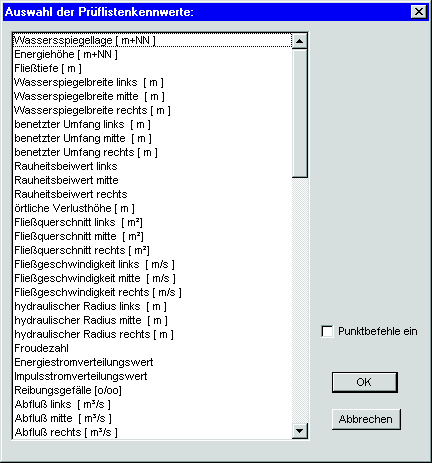
\includegraphics[width=0.8\textwidth]{Prueflistenkennwerte}
   \caption{Auswahl der Pr\"{u}flistenkennwerte}
   \label{Fortgeschrittene Abb Prueflistenkennwerte}
\end{figure}


\subsection{Wasserspiegel einf\"{u}gen}

Bei jeder Berechnung erfolgt, sofern in den Steueroptionen der Berechnung angegeben, ein Eintrag der errechneten
Wasserspiegellagen in die Querprofile. Dabei werden die bereits vorhandenen Wasserspiegellagen fr\"{u}herer Berechnungen
gel\"{o}scht.

Die Eintr\"{a}ge k\"{o}nnen auch einzeln \"{u}ber das Men\"{u} \menu{\marrow \underline{E}rgebnisse \marrow \underline{W}asserspiegel...
\marrow \underline{L}\"{o}\-schen in allen Querprofilen} aus den Querprofilen entfernt werden. In gleicher Weise lassen sich
\"{u}ber das Men\"{u} \menu{\marrow \underline{E}inf\"{u}gen in Querprofil} die Wasserspiegellagen von Berechnungsvarianten auch von
Hand in die Querprofile eingetragen. Dies ist sinnvoll, wenn kein automatischer Eintrag bei der Berechnung vereinbart
wurde, oder die Wasserspiegellagen verschiedener Varianten im Profil verglichen werden sollen.


\clearpage
%%%%%%%%%%%%%%%%%%%%%%%%%%%%%%%%%%%%%%%%%%%%%%%%%%%%%%%%%%%%%%%%%%%%%%%%%%%%%%%%%%%%%%%%%%%%%%%%%%%%%%%%%%%%%%%%%%%%%%%%%%%%
\section{Plotten}
%%%%%%%%%%%%%%%%%%%%%%%%%%%%%%%%%%%%%%%%%%%%%%%%%%%%%%%%%%%%%%%%%%%%%%%%%%%%%%%%%%%%%%%%%%%%%%%%%%%%%%%%%%%%%%%%%%%%%%%%%%%%
\begin{figure}[hbt]
   \centering
   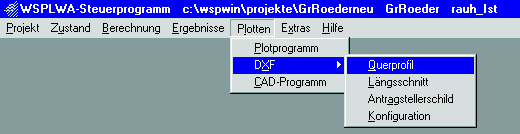
\includegraphics[width=0.8\textwidth]{MenuePlotten}
   \caption{Der Men\"{u}punkt \menu{\marrow P\underline{l}otten}}
   \label{Fortgeschrittene Abb MenuePlotten}
\end{figure}


\subsection{Plotprogramm}

Zu \wspwin{} gibt es seit 1999 ein eigenst\"{a}ndiges Plotprogramm \afz{\wspwin{}-Plotter}, \"{u}ber das Sie in einer
Windowsoberfl\"{a}che L\"{a}ngs- und Querprofile direkt formatieren und plotten k\"{o}nnen. Der Umweg \"{u}ber die Erzeugung von
\datei{*.dxf}-Dateien und ein zus\"{a}tzliches CAD-Programm entf\"{a}llt hierdurch.
Eine ausf�hrliche Beschreibung finden Sie im Handbuch des Plotprogramms.


\subsection{DXF-Dateien erzeugen}

Mit Hilfe von \wspwin{} k\"{o}nnen sowohl f\"{u}r die L\"{a}ngsschnitte, als auch f\"{u}r die Querprofile \datei{*.dxf}-Dateien erstellt
werden, die sich in einem CAD-Programm bearbeiten und plotten lassen. Vor dem Erstellen der Dateien lassen sich
verschiedene Voreinstellungen zur Art und Weise der Darstellung in der CAD-Datei vornehmen. F\"{u}r L\"{a}ngsschnitte existieren
im allgemeinen bereits Voreinstellungen aus den L\"{a}ngsschnittdateien. Bei Querprofilen sind diese komplett neu zu
erstellen.

\"{U}ber die Men\"{u}punkte \menu{\marrow P\underline{l}otten \marrow D\underline{X}F \marrow \underline{Q}uerprofil} bzw.
\menu{\marrow \underline{L}\"{a}ngsschnitt} gelangen Sie in einen Dialog zur Auswahl des Querprofils oder der
L\"{a}ngsschnittdatei. \"{U}ber die Schalter \schalter{Plotten} bzw. \schalter{OK} wird ein Programm gestartet, das die
\datei{*.dxf}-Datei aus dem markierten Profil erzeugt. Zum besseren Verst\"{a}ndnis der Eingabeparameter werden zun\"{a}chst
einige Begriffe erl\"{a}utert:
\begin{description}
   \item[Profillinie:] Sie ergibt sich aus den $(y,z)$-Koordinaten eines Datensatzes der Profildatei.
   \item[Stationslinie:] Senkrechte Linie von der Profillinie zum Schriftfeld
   \item[Schriftfeld:] Im Schriftfeld werden die Daten und Ergebnisse eingetragen. Sie dienen zur Erl\"{a}uterung der
      grafischen Darstellung
   \item[Symbole:] Alle Zeichnungseintr\"{a}ge, die durch einen Datensatz erfolgen und keine Profillinie sind, werden als
      Symbole bezeichnet.
\end{description}
Der zu erstellende Plot besteht aus drei Elementen, dem Stempel, dem Schriftfeld und der eigentlichen Zeichnung.
\begin{figure}[hbt]
   \centering
   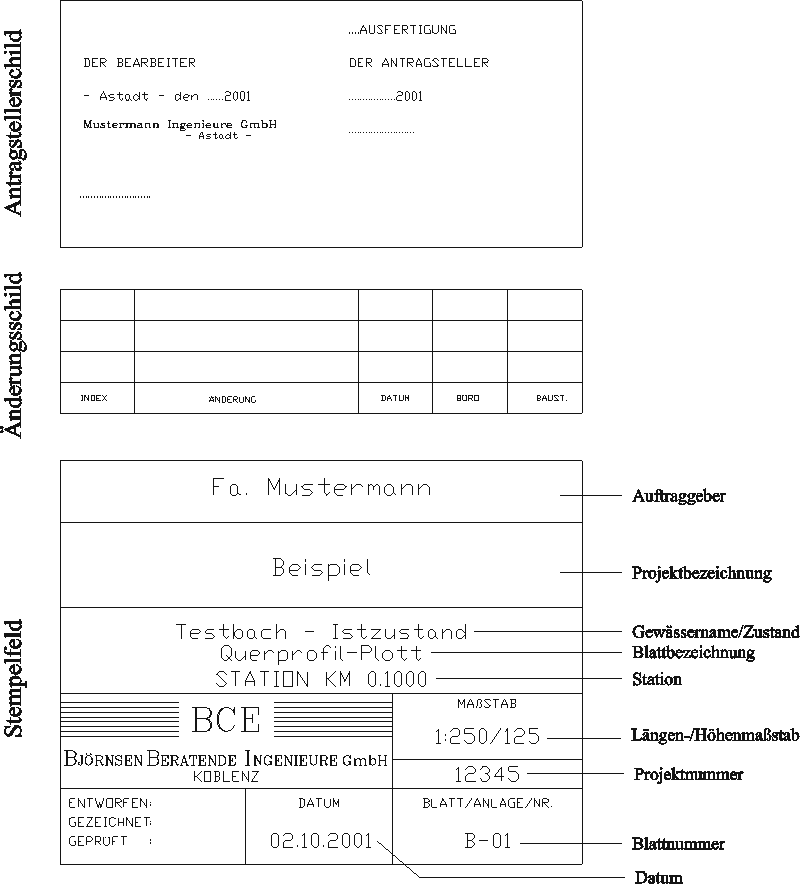
\includegraphics[width=0.9\textwidth]{Stempelfeld}
   \caption{Stempelfeld mit optionalem \"{A}nderungs- und Antragstellerschild. Zus\"{a}tzlich kann noch eine Legende dargestellt
            werden.}
   \label{Fortgeschrittene Abb Stempelfeld}
\end{figure}

\subsubsection{Stempelfeld}
In die Zeichnung wird grunds\"{a}tzlich ein Stempel (Abbildung~\ref{Fortgeschrittene Abb Stempelfeld} unten)
eingetragen. Zus\"{a}tzlich kann wahlweise ein \"{A}nderungsschild, ein Antragstellerschild oder eine Legende in die Zeichnung
aufgenommen werden. Die Definitionen der Eintragungen im Antragstellerschild sind unter dem Men\"{u}punkt \menu{ \marrow
P\underline{l}otten \marrow D\underline{X}F \marrow Antr\underline{a}gstellerschild} vorzunehmen.

Im Auswahldialog f\"{u}r den zu plottenden L\"{a}ngs- oder Querschnitt k\"{o}nnen Sie \"{u}ber die Schaltfl\"{a}che \schalter{Plotoptionen}
Einstellung zur Darstellung in der Zeichnungsdatei vornehmen. Sie werden zun\"{a}chst in den Dialog \dialog{Bearbeiten der
Stempeldaten} (vgl. Abbildung~\ref{Fortgeschrittene Abb PlottenStempeldaten}) gef\"{u}hrt. Hier sind die Daten f\"{u}r das
Stempelfeld gem\"{a}{\ss} Abbildung~\ref{Fortgeschrittene Abb Stempelfeld} zu vereinbaren. Weiterhin kann eine
Zeichnungs\"{u}berschrift angegeben werden, die sp\"{a}ter \"{u}ber der Schnittdarstellung auf Ihrer Zeichnung erscheint.

\begin{figure}[hbt]
   \centering
   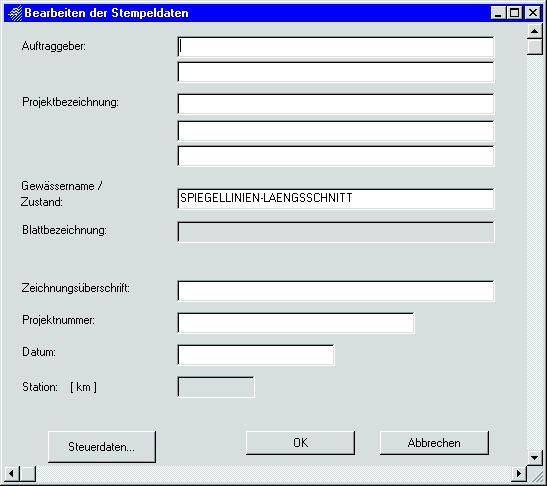
\includegraphics[width=0.9\textwidth]{PlottenStempeldaten}
   \caption{Eingabe der Stempeldaten}
   \label{Fortgeschrittene Abb PlottenStempeldaten}
\end{figure}

\"{U}ber die Schaltfl\"{a}che \schalter{Steuerdaten...} werden die Dialogmasken zur Festlegung Art und Weise der
Stationsbeschriftung aufgerufen (Abbildungen~\ref{Fortgeschrittene Abb Stationsbeschriftung_I} und \ref{Fortgeschrittene Abb Stationsbeschriftung_II}).

\subsubsection{Schriftfeld}
Die Darstellung im Schriftfeld beinhaltet die tabellarische Auflistung der berechneten oder eingegebenen Daten. Das
Schriftfeld besteht aus mindestens zwei Zeilen. Eine Zeile ist jeweils in einen Block f\"{u}r die Bezeichnung und einen f\"{u}r
die dazugeh\"{o}rigen Daten unterteilt. Der erste Datensatz der Profildatei (Gel\"{a}ndeh\"{o}he) wird dabei stets durch zwei
Schriftfeldzeilen, der Stationierungszeile und der Datenzeile, dargestellt. F\"{u}r alle weiteren Datens\"{a}tze ist die
M\"{o}glichkeit gegeben, Stations- und H\"{o}henwerte in dieselbe Schriftfeldzeile einzutragen. Dabei werden Stationswerte stets
links und H\"{o}henwerte stets rechts vom Bezugspunkt eingetragen.
\begin{figure}
   \centering
      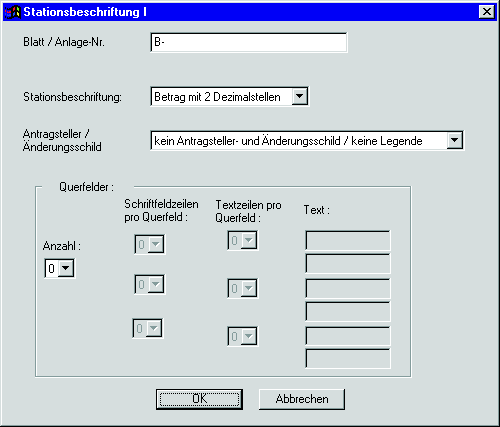
\includegraphics[width=0.75\textwidth]{PlottenStationsbeschriftung_I}
      \caption{Erstes Dialogfenster zur Stationsbeschriftung}
      \label{Fortgeschrittene Abb Stationsbeschriftung_I}
\end{figure}

\begin{figure}
    \centering
      \includegraphics[width=0.75\textwidth]{PlottenStationsbeschriftung_II}
      \caption{Zweites Dialogfenster zur Stationsbeschriftung}
      \label{Fortgeschrittene Abb Stationsbeschriftung_II}
\end{figure}

\begin{sidewaysfigure}
   \centering
   \includegraphics[width=0.9\textwidth]{Laengsschnittplott}
   \caption{L\"{a}ngsschnittplott mit verschiedenen Schriftfelddarstellungen}
   \label{Fortgeschrittene Abb Laengsschnittplott}
\end{sidewaysfigure}

Die Schaltfl\"{a}che \schalter{Steuerdaten} im Dialog \dialog{Bearbeiten der Stempeldaten} f\"{u}hrt sie in die Umgebung zur
Festlegung der Darstellungsform des Schriftfeldes. Mehreren Schriftfeldzeilen kann mit Hilfe von Querfeldern eine
Beschriftung voran gestellt werden. Neben der Anzahl der Querfelder, mu{\ss} dazu auch die Anzahl der Schriftfeldzeilen
angegeben werden, die das Querfeld verbinden soll. Jedem Querfeld k\"{o}nnen ein oder zwei Textzeilen zugeordnet werden.

Die Bezeichnung einer Schriftfeldzeile (d.h. eines Datensatzes) kann bis zu zwei Textzeilen lang sein. F\"{u}r eine schmale
Schriftfeldzeile wird der Text, wenn er aus zwei Textzeilen besteht, verkleinert. Manche Schriftfeldzeilen bestehen nur
aus Erl\"{a}uterungstext, andere haben in der Regel auch eine Ma{\ss}einheit. Daher kann dieses Feld weiter unterteilt werden. Auf
der linken Seite steht dann die Bezeichnung, auf der rechten Seite die Ma{\ss}einheit und der Linientyp, wenn die Werte
grafisch dargestellt werden. Damit ergeben sich folgende Darstellungsformen einer Schriftfeldzeile:
\begin{itemize}
   \item keine Schriftfeldzeile
   \item schmale Schriftfeldzeile ohne Unterteilung (vgl. Datensatz \afz{Schleppspannung} in
         Abbildung~\ref{Fortgeschrittene Abb Laengsschnittplott})
   \item schmale Schriftfeldzeile mit Unterteilung (vgl. Datensatz~\afz{Wasserspiegel} in
         Abbildung~\ref{Fortgeschrittene Abb Laengsschnittplott})
   \item breite Schriftfeldzeile ohne Unterteilung (vgl. Datens\"{a}tze~\afz{B\"{o}\-schung li.} und \afz{B\"{o}\-schung re.} in
         Abbildung~\ref{Fortgeschrittene Abb Laengsschnittplott}
   \item breite Schriftfeldzeile mit Unterteilung (vgl.
         Ab\-bil\-dung~\ref{Fortgeschrittene Abb Laengsschnittplott}, Datensatz~\afz{Sohlh\"{o}he})
\end{itemize}

Blattgr\"{o}{\ss}e, Ma{\ss}stab und Schriftfeldabstand zum Zeichnungsrand werden im Dialog \dialog{Stationsbeschriftung II}
festgelegt. Weiterhin ist die Bezugsh\"{o}he einzugeben, \"{u}ber der der Auftrag der Profile erfolgen soll. Eine Beschriftung der
Bezugsh\"{o}he kann mit Hilfe von \checkbox{Unterdr\"{u}cken der Bezugsh\"{o}he} unterbunden werden. Zus\"{a}tzlich zu dem Voranstellen
einer Beschriftung in einem Querfeld vor mehrere Schriftfeldzeilen kann die Zusammengeh\"{o}rigkeit von Daten auch durch
Rahmen kenntlich gemacht werden. Dazu ist im unteren Teil der Dialogmaske die Anzahl der Unterteilungen des Schriftfeldes
anzugeben. Maximal sind f\"{u}nf Unterteilungen m\"{o}glich. Jeder Unterteilung ist danach die gew\"{u}nschte Anzahl der
Schriftfeldzeilen zuzuordnen. Wird die Option \checkbox{Unterdr\"{u}cken von Werten} aktiviert, so werden nur die Daten
dargestellt, f\"{u}r deren Beschriftung ausreichend Platz vorhanden ist.
\begin{figure}[hbt]
   \centering
   \includegraphics[width=1.0\textwidth]{PlottenOptionenDatensatz}
   \caption{Dialog zur Darstellung der Datens\"{a}tze}
   \label{Fortgeschrittene Abb OptionenDatensatz}
\end{figure}





\subsubsection{Darstellung der Daten}
Der letzte Dialog (Abbildung~\ref{Fortgeschrittene Abb OptionenDatensatz}) betrifft die Darstellung der einzelnen
Datens\"{a}tze auf der Zeichnung. Die Darstellung der Daten im Schriftfeld kann auf verschiedene Art und Weise erfolgen. Dies
betrifft sowohl das Zahlenformat, die Ausrichtung als auch die Datenmenge. Im Dialogfenster \dialog{Optionen Datensatz}
(Abbildung~\ref{Fortgeschrittene Abb OptionenDatensatz}) werden dazu zun\"{a}chst alle vorhandenen Datens\"{a}tze in einer Liste
links oben angezeigt. Durch Auswahl eines Datensatzes kann ihm das entsprechende Datenformat zugewiesen werden. Soll der
komplette Datensatz im Schriftfeld nicht dargestellt werden, so ist aus der Liste \feld{Schriftfeldzeilen} \afz{keine
Schriftfeldzeile} auszuw\"{a}hlen.

Unter dem Listenfeld mit den Datens\"{a}tzen finden Sie eine Auswahlm\"{o}glichkeit f\"{u}r das Darstellungsformat Ihrer Profillinien.
Die $y$- und $z$-Werte k\"{o}nnen jeweils alle, gar nicht oder als Auswahl dargestellt werden. Die Auswahl einzelner Werte
erfolgt ein einem gesonderten Dialog. In gleicher Weise l\"{a}{\ss}t sich auch die Darstellung der H\"{o}henlinien beeinflussen.

Darunter finden Sie das Listenfeld zur Darstellungsform der Schriftfeldzeilen. Der Text kann waagerecht und senkrecht in
verschiedenen Schriftgr\"{o}{\ss}en eingetragen werden.
\begin{quote}
   \begin{tabular}{ll}
      kleine Schrift:          &    $1,0\unit{mm}$ \\
      normale Schrift: \qquad  &    $2,0\unit{mm}$ \\
      Gro{\ss}e Schrift:           &    $3,0\unit{mm}$
   \end{tabular}
\end{quote}
Werden sowohl $y$- als auch $z$-Werte an einer Station angezeigt, so erfolgt die Darstellung der Daten \"{u}bereinander (vgl.
Abbildung~\ref{Fortgeschrittene Abb Laengsschnittplott} \afz{Energieh\"{o}he}). Es ist jedoch auch eine Ausgabe der $z$-Werte
auf der H\"{o}he der Station m\"{o}glich. Die Daten werden im Normalfall an senkrechten Linien im Schriftfeld ausgerichtet. Sie
lassen sich so einer exakten Position zuordnen. Besonders bei einer H\"{a}ufung von Daten in bestimmten Bereichen kann es
sinnvoll sein, nicht alle Linien darstellen zu lassen, da es hier u.U. zu einer \"{U}berschneidung in der Darstellung kommt.
Haben sie zur Darstellung der Linien im Datensatz \afz{Sohlh\"{o}he} bereits eine Auswahl getroffen, so kann diese Auswahl in
den anderen Datens\"{a}tzen \"{u}bernommen werden. Nach dem Best\"{a}tigen der Eingabe mit \schalter{OK} gelangen Sie zur\"{u}ck in das
Dialogfenster \dialog{Bearbeiten der Stempeldaten}.


\subsubsection{Plotten Konfiguration}
\wspwin{} wird mit einer Plotterkonfigurationsdatei geliefert. Die Konfigurationsdatei dient dazu, einzelnen Layern Stifte
unterschiedlicher Strichst\"{a}rke oder Farbe zuzuordnen. Dabei werden den einzelnen Layern (z.B. Gel\"{a}ndelinie, Text) die
Nummern der Stifte des Plotters zugewiesen. Die mitgelieferte Plotterkonfigurationsdatei \datei{plotter.cfg} ist auf einen
speziellen Farbplotter angepa{\ss}t, bei dem Sie unter dem Men\"{u} \menu{\marrow P\underline{l}otten \marrow D\underline{X}F
\marrow \underline{K}onfiguration} den einzelnen Layern verschiedene Farben (z.B. Sohlh\"{o}he blau) zuweisen k\"{o}nnen. Eine
\"{U}bersicht welche Linientypen in welchen Layern repr\"{a}sentiert werden, findet sich in Abbildung~\ref{Fortgeschrittene Abb
LinienLayer}.
\begin{figure}[hbt]
   \centering
   \includegraphics[width=0.7\textwidth]{LinienLayer}
   \caption{Linientypen und zugeordnete Layer}
   \label{Fortgeschrittene Abb LinienLayer}
\end{figure}


\subsection{CAD-Programm}

Zur Einsicht und zum Bearbeiten der erstellten \datei{*.dxf}-Dateien kann \"{u}ber diesen Men\"{u}punkt ein externes CAD-Programm
gestartet werden. Im Men\"{u} \menu{\marrow E\underline{x},0tras} sind dazu die entsprechenden Einstellungen gem\"{a}{\ss}
Abschnitt~\ref{Installation Subsec Verzeichnisse} vorzunehmen.
    %  Kapitel  5
   \graphicspath{{Sonderprofile/eps/}} \cleardoublepage
%%%%%%%%%%%%%%%%%%%%%%%%%%%%%%%%%%%%%%%%%%%%%%%%%%%%%%%%%%%%%%%%%%%%%%%%%%%%%%%%%%%%%%%%%%%%%%%%%%%%%%%%%%%%%%%%%%%%%%%%%%%%

\chapter{Sonderprofile}

%%%%%%%%%%%%%%%%%%%%%%%%%%%%%%%%%%%%%%%%%%%%%%%%%%%%%%%%%%%%%%%%%%%%%%%%%%%%%%%%%%%%%%%%%%%%%%%%%%%%%%%%%%%%%%%%%%%%%%%%%%%%

%%%%%%%%%%%%%%%%%%%%%%%%%%%%%%%%%%%%%%%%%%%%%%%%%%%%%%%%%%%%%%%%%%%%%%%%%%%%%%%%%%%%%%%%%%%%%%%%%%%%%%%%%%%%%%%%%%%%%%%%%%%%
\section{Profile mit R\"{u}ckspr\"{u}ngen}
%%%%%%%%%%%%%%%%%%%%%%%%%%%%%%%%%%%%%%%%%%%%%%%%%%%%%%%%%%%%%%%%%%%%%%%%%%%%%%%%%%%%%%%%%%%%%%%%%%%%%%%%%%%%%%%%%%%%%%%%%%%%

Profile mit R\"{u}ckspr\"{u}ngen k\"{o}nnen wie Normalprofile eingegeben werden. Die Berechnung erfolgt mit Hilfe des
\autor{Gauss}'schen Algorithmus f\"{u}r die Fl\"{a}chenberechnung. Hierbei werden die Schnittpunkte zwischen horizontaler
Wasserspiegellage und Profilpolygon ermittelt und der Fl\"{a}cheninhalt berechnet.
\begin{figure}[htpb]
   \centering
   \includegraphics[width=0.8\textwidth]{Gaussprofil}
   \caption{Profil mit auskragender Fahrbahnplatte}
   \label{Sonderprofile Abb Fahrbahnplatte}
\end{figure}
Die Eingabereihenfolge der Profilpunkte wird aus Abbildung~\ref{Sonderprofile Abb Fahrbahnplatte} ersichtlich. Eine
Unterteilung des Abflu{\ss}querschnitts in Vorl\"{a}nder und Flu{\ss}bett wird nicht ber\"{u}cksichtigt. Die Berechnung erfolgt f\"{u}r die im
Flu{\ss}schlauch angegebenen Rauheiten.

Im Profileditor (alphanumerisch und grafisch) werden Profile mit R�ckspr�ngen in den Schl�sseldaten mit 'GaussR�cksprung' gekennzeichnet. Dar�berhinaus sind alle Profilpunkte, welche an einer senkrechten Wand oder einem R�cksprung liegen, im Textfeld rot markiert.

\clearpage
%%%%%%%%%%%%%%%%%%%%%%%%%%%%%%%%%%%%%%%%%%%%%%%%%%%%%%%%%%%%%%%%%%%%%%%%%%%%%%%%%%%%%%%%%%%%%%%%%%%%%%%%%%%%%%%%%%%%%%%%%%%%
\section{Niedrigwasserrinnen}
%%%%%%%%%%%%%%%%%%%%%%%%%%%%%%%%%%%%%%%%%%%%%%%%%%%%%%%%%%%%%%%%%%%%%%%%%%%%%%%%%%%%%%%%%%%%%%%%%%%%%%%%%%%%%%%%%%%%%%%%%%%%
Eine Variante f\"{u}r die Eingabe besteht darin, einen Teilabflu{\ss}querschnitt des Flu{\ss}schlauchs in integraler Form einzugeben
(Abbildung~\ref{Sonderprofile Abb integraleProfileingabe}). Von dem Teilabflu{\ss}querschnitt werden die planimetrierte Fl\"{a}che (FP), der Umfang (UP) und die Wasserspiegelbreite (BP) ben\"{o}tigt. Der linke und rechte Uferanschnittpunkt des zum
Teilabflu{\ss}querschnitt geh\"{o}renden Wasserspiegels sind dabei als Profilpunkte durch Koordinatenangabe festzulegen. Die f\"{u}r
diese Berechnungsart erforderlichen zus\"{a}tzlichen Daten sind im Datensatz \afz{Niedrigwasserrinne} einzutragen.
\begin{figure}[hbt]
   \centering
   \includegraphics[width=0.9\textwidth]{ProfilaufnahmeIntegral}
   \caption{Querprofildaten - Eingabe teilweise in Koordinaten, teilweise in integraler Form}
   \label{Sonderprofile Abb integraleProfileingabe}
\end{figure}


\clearpage
%%%%%%%%%%%%%%%%%%%%%%%%%%%%%%%%%%%%%%%%%%%%%%%%%%%%%%%%%%%%%%%%%%%%%%%%%%%%%%%%%%%%%%%%%%%%%%%%%%%%%%%%%%%%%%%%%%%%%%%%%%%
\section{Br\"{u}cken}
%%%%%%%%%%%%%%%%%%%%%%%%%%%%%%%%%%%%%%%%%%%%%%%%%%%%%%%%%%%%%%%%%%%%%%%%%%%%%%%%%%%%%%%%%%%%%%%%%%%%%%%%%%%%%%%%%%%%%%%%%%%

An Br\"{u}cken werden nach~\cite{BWK1999} folgende Abflu{\ss}zust\"{a}nde unterschieden:
\begin{quote}
   \begin{itemize}
      \item Freier Abflu{\ss}
      \item R\"{u}ckgestaute Br\"{u}cke mit freiem Abflu{\ss} unter der Br\"{u}cke
      \item R\"{u}ckgestaute Br\"{u}cke und Druckabflu{\ss}
      \item Vollkommener \"{U}berfall und Druckabflu{\ss} unter der Br\"{u}cke
      \item \"{U}berstr\"{o}men und Druckabflu{\ss} unter der Br\"{u}cke
   \end{itemize}
\end{quote}


\subsection{Freier Abfluss}

Liegt der Wasserspiegel sowohl vor, als auch hinter der Br\"{u}cke unterhalb deren Konstruktionsunterkante, so spricht man von
einem freien Abflu{\ss}. Durch Einbauten im Flie{\ss}querschnitt in Form von Br\"{u}ckenpfeilern kann hier eine Wasserspiegelanhebung
entstehen. Diese l\"{a}{\ss}t sich mit Hilfe der Pfeilerstauformeln nach \autor{Rehbock} oder \autor{Yarnell} berechnen.
\begin{figure}[hbt]
   \centering
   \includegraphics[width=0.8\textwidth]{Pfeilerstau}
   \caption{Pfeilerstau bei str\"{o}mendem Abflu{\ss}}
   \label{Sonderprofile Abb Pfeilerstau}
\end{figure}

Durch \"{U}berspringen des Br\"{u}ckenprofils~$(i-1)$ wird zun\"{a}chst die \afz{ungest\"{o}rte} Wasserspiegelh\"{o}he im Profil~$(i)$ und
durch Interpolation zwischen den Profilen~$(i-2)$ und $(i)$ eine fiktive Wasserspiegelh\"{o}he im Querschnitt~$(i-1)$
berechnet. F\"{u}r diese Referenzh\"{o}he wird dann der Flie{\ss}querschnitt sowohl f\"{u}r das Br\"{u}ckenprofil als auch f\"{u}r das
unterwasserseitige Profil~$(i-2)$ ermittelt. Werden diese Flie{\ss}fl\"{a}chen mit $A'_{i-1}$ und $A'_{i-2}$ bezeichnet, so lautet
der Ansatz f\"{u}r das Verbauungsverh\"{a}ltnis
\begin{equation}
   \alpha_V = \frac{A'_{i-2} - A'_{i-1}}{A'_{i-2}}
\end{equation}

Mit diesem Verbauungsverh\"{a}ltnis, dem vorzugebenden Pfeilerformbeiwert und den hydraulischen Kennwerten des unterstromigen
Querschnitts kann die Aufstauh\"{o}he $dz$ berechnet und zu der ermittelten \afz{ungest\"{o}rten} Wasserspiegellage addiert
werden. Wie f\"{u}r jeden anderen Querschnitt wird die \autor{Froude}'sche Zahl auch f\"{u}r das Br\"{u}ckenprofil berechnet. Ergibt
sich f\"{u}r die Engstelle ein Wert $Fr > 1$, so liegt im Bereich der Verbauung ein Flie{\ss}wechsel vor. In diesem Fall wird die
oberstromige Wasserspiegellage mit Hilfe des Extremalprinzips berechnet.

Aus der gew\"{a}hlten Berechnungsart ergibt sich, da{\ss} das unterstromige Querprofil bei einer Br\"{u}cke (bis auf die den
Flu{\ss}querschnitt einengenden Einbauten) genau dem Br\"{u}ckenprofil entsprechen mu{\ss}. Der Flie{\ss}querschnitt darf hier keinesfalls
kleiner als in der Br\"{u}cke selbst sein, sonst ergibt sich ein negatives Verbauungsverh\"{a}ltnis.

\subsubsection{Pfeilerstauformel nach Rehbock}
Die allgemeine Form der Pfeilerstauformel nach \autor{Rehbock} lautet:
\begin{equation}
   dz = \alpha_V \cdot \left( \delta - \alpha_V \cdot (\delta - 1) \right) \cdot
        \left( 0,4 + \alpha_V + 9\alpha_V^3 \right) \cdot \left( 1 + Fr_{i-2}^2 \right) \cdot h_{k,i-1}
\end{equation}
Die Pfeilerformbeiwerte k\"{o}nnen Abbildung~\ref{Sonderprofile Abb RehbockBeiwerte} entnommen werden.

\begin{figure}[hpbt]
   \centering
   \includegraphics[width=0.75\textwidth]{Rehbock}
   \caption{Pfeilerformbeiwerte nach \autor{Rehbock}}
   \label{Sonderprofile Abb RehbockBeiwerte}
\end{figure}

Hinsichtlich der Anwendbarkeit der \autor{Rehbock}-Formel auf Gerinneeinbauten in Form von Widerlagern liegen
Untersuchungen~\cite{Schwarze} an Modellgerinnen mit Rechteck- und Trapezquerschnitten vor. Erwartungsgem\"{a}{\ss} ergab sich f\"{u}r
den seitlichen Verbau des Flie{\ss}querschnitts allgemein ein kleinerer Aufstau $dz$ als bei einem fl\"{a}chengleichen
Mittelpfeilerverbau. Andererseits stellte sich heraus, da{\ss} bei \"{U}berschreitung eines von der Gerinneform abh\"{a}ngigen
Verbauungsverh\"{a}ltnisses die \autor{Rehbock}-Formel zu kleine Werte liefert. Als Grenzwerte des Verbauungsverh\"{a}ltnisses,
bis zu dem bei Widerlagerverbau die \autor{Rehbock}-Formel auf der sicheren Seite liegende Ergebnisse liefert, ergaben
sich nach~\cite{Schwarze}:
\begin{quote}
   \begin{tabular}{lll}
      Rechteckgerinne:  &  $\alpha_V = 0,23$ \\
      Trapezgerinne :   &  $\alpha_V = 0,34$ & (B\"{o}schungsneigung $1:2$)\\
                        &  $\alpha_V = 0,44$ & (B\"{o}schungsneigung $1:3$)
   \end{tabular}
\end{quote}


\subsubsection{Pfeilerstau nach Yarnell}
Die durch Einbauten in Form von Pfeilern verursachte Wasserspiegelanhebung $dz$ kann alternativ auch f\"{u}r den freien und
str\"{o}menden Abflu{\ss} in \"{a}hnlicher Weise wie oben beschrieben mit Hilfe der Formel von \autor{Yarnell} berechnet werden:
\begin{equation}
   dz = 2\sigma \cdot \left( \sigma + 10 \cdot \frac{h_{k,i-1}}{h_u} - 0,6 \right) \cdot
        \left(\alpha_V + 15\alpha_V^4 \right) \cdot h_{k,i-1}
\end{equation}
Die zugeh\"{o}rigen Pfeilerformbeiwerte $\sigma$ k\"{o}nnen Tabelle~\ref{Sonderprofile Tab Yarnell} entnommen werden.
\begin{table}[hp]
   \centering
   \input{Sonderprofile/tab/Yarnell.tab}
   \caption{Pfeilerformbeiwerte $\sigma$ nach \autor{Yarnell}}
   \label{Sonderprofile Tab Yarnell}
\end{table}

%%dz  = Anhebung der ungest\"{o}rten Wasserspiegelh\"{o}he im Profil(i) in m av = Verbauungsverh\"{a}ltnis = verbaute Fl\"{a}che/
%%unverbaute Fl\"{a}che s = Pfeilerformbeiwert nach YARNELL

Wie die \autor{Rehbock}'sche Staugleichung ist diese Gleichung nur f\"{u}r den freien Abflu{\ss} ohne Flie{\ss}wechsel g\"{u}ltig.


\subsection{R\"{u}ckgestaute Br\"{u}cken}

Die Berechnung r\"{u}ckgestauter Br\"{u}cken ohne \"{U}berstr\"{o}mung erfolgt in gleicher Weise wie in Abschnitt~\ref{Sonderprofile Subse
UeberstroemteBruecken} beschrieben. Der Anteil der \"{U}berstr\"{o}mung $Q_{Rest}$ ist dann jedoch null.


\subsection{Mehrfeldbr\"{u}cken}
\label{Sonderprofile Subsec Mehrfeldbruecken}

Der Durchflu{\ss} durch Br\"{u}cken mit mehreren Flut\"{o}ffnungen kann wie eine Stromverzweigung mit Hilfe einer iterativen
Stromaufteilungsberechnung nach Abschnitt~\ref{Sonderprofile Sec VerzweigteSysteme} berechnet werden.

Bei normalen relativ kurzen Br\"{u}ckenbauwerken ist jedoch die Kenntnis der einzelnen Teilstr\"{o}me durch die jeweiligen
Flut\"{o}ffnungen meist nicht erforderlich. Der Aufwand f\"{u}r die Verzweigungsberechnung kann in diesem Fall durch eine
integrale Berechnungsweise ersetzt werden, wobei sich die Differenzierung auf maximal 3~Teilstr\"{o}me beschr\"{a}nkt.

Zweckm\"{a}{\ss}igerweise ist der Br\"{u}ckenabflu{\ss} wie der Abflu{\ss} im Normalprofil in Vorland- und Flu{\ss}bettabflu{\ss} zu unterteilen. In
Abh\"{a}ngigkeit von der Wasserspiegellage werden die hydraulisch relevanten Kenngr\"{o}{\ss}en der einzelnen Flut\"{o}ffnungen wie
Spiegelbreite, benetzter Umfang und Durchflu{\ss}fl\"{a}che berechnet und als skalare Gr\"{o}{\ss}en zum Teilabflu{\ss}querschnitt des
Vorlandes bzw. Flu{\ss}bettes aufsummiert. \"{A}hnlich wie bei normalen gegliederten Profilen ist die Zuordnung der einzelnen
Flut\"{o}ffnungen zum Teilstrom Vorland oder Teilstrom Flu{\ss}bett durch die Dateneingabe vorzugeben.

F\"{u}r jede in der H\"{o}he begrenzte Flut\"{o}ffnung ist ein gesondertes Querprofil einzugeben, wobei alle Profiltypen verwendet
werden k\"{o}nnen. Durch diese Art der Eingabe bestehen keine zus\"{a}tzlichen Beschr\"{a}nkungen hinsichtlich Anzahl und Form der
einzelnen Flut\"{o}ffnungen einer Mehrfeldbr\"{u}cke. Lediglich die Gesamtzahl aller Querprofile eines Berechnungsabschnittes ist
aus Speicherplatzgr\"{u}nden begrenzt.

Die integrale Mehrfeldbr\"{u}ckenberechnung beschr\"{a}nkt sich auf die explizite Berechnung von drei Teilstr\"{o}men, f\"{u}r die
hydraulische Ersatzquerschnitte unter Beachtung ver\"{a}n\-derlicher Rauheitsbeiwerte gebildet werden. Da der Abstand zwischen
den Flut\"{o}ffnungen nicht in die Berechnung eingeht (die Kombination von Mehrfeldbr\"{u}ckenberechnung und Pfeilerstauberechnung
ist nicht zul\"{a}ssig) kann diese Art der Berechnung nur als N\"{a}herung betrachtet werden. F\"{u}r genauere Berechnungen ist eine
Verzweigungsberechnung zu w\"{a}hlen. Zur Erfassung zus\"{a}tzlicher \"{o}rtlicher Verluste bei Mehrfeldbr\"{u}cken sind entsprechende
Verlustbeiwerte festzulegen.


\subsection{\"{U}berstr\"{o}mte Br\"{u}cken}
\label{Sonderprofile Subse UeberstroemteBruecken}

Wenn die hydraulische Kapazit\"{a}t von Br\"{u}cken oder Durchl\"{a}ssen \"{u}berschritten wird oder wenn der Unterwasserstand eine Br\"{u}cke
einstaut, dann findet ein Abflu{\ss} durch die Br\"{u}cke ohne Freibord statt (Sonderbauwerk mit vollaufendem Querschnitt).

In diesen F\"{a}llen staut sich das Wasser vor der Br\"{u}cke, bis die zum Abflu{\ss} der ankommenden Wassermenge erforderliche
Energieh\"{o}he erreicht ist. Der Wasserstand vor der Br\"{u}cke steigt mit der im Abflu{\ss}querschnitt erforderlichen
Geschwindigkeitsh\"{o}he quadratisch mit der Flie{\ss}geschwindigkeit an, d.h. bei sehr gro{\ss}en Geschwindigkeiten k\"{o}nnen sich
Stauh\"{o}hen ergeben, die h\"{o}her sind als die Oberkante des Bauwerkes. In diesen F\"{a}llen wird die Br\"{u}cke \"{u}berflutet, d.h. die
theoretische Stauh\"{o}he stellt sich nicht ein, sondern es findet eine Entlastung \"{u}ber die Br\"{u}cke statt.

Um unrealistische Spr\"{u}nge in der Wasserspiegellage zu vermeiden, k\"{o}nnen im Rahmen von Spiegellinienberechnungen die
hydraulischen Oberkanten der Br\"{u}cken ber\"{u}cksichtigt werden. Von Bedeutung wird dabei die Wassermengenaufteilung. Ein Teil
der ankommenden Wassermenge wird weiterhin den Br\"{u}ckenquerschnitt durchflie{\ss}en, der \"{u}berwiegende Teil wird sich jedoch als
\"{U}berfallstr\"{o}mung \"{u}ber das Bauwerk ergie{\ss}en.

Hydraulisch handelt es sich bei dem Abflu{\ss}anteil im Br\"{u}ckenquerschnitt um einen unvollkommenen Ausflu{\ss} aus einer
begrenzten \"{O}ffnung. Nach~\cite{PressSchroeder} gilt f\"{u}r diesen Fall:
\begin{equation}
   Q_{Br"ucke} = \alpha_B \cdot A \cdot \sqrt{2g \cdot (h_o - h_u)}
\end{equation}
\begin{quote}
   \begin{tabular}{lll}
   mit   &  $h_o$      &  Stauh\"{o}he vor der Br\"{u}cke \\
         &  $h_u$      &  Unterwasserstand \\
         &  $A$        &  Flie{\ss}querschnitt der Br\"{u}cke \\
         &  $\alpha_B$ &  Abflu{\ss}zahl
   \end{tabular}
\end{quote}
Der Gesamtabflu{\ss} setzt sich aus dem Anteilen des Druckabflusses und der \"{U}berstr\"{o}mung zusammen. Der Anteil der \"{U}berstr\"{o}mung
betr\"{a}gt demnach:
\begin{equation}
   Q_{Rest} = Q_{ges} - Q_{Br"ucke}
\end{equation}
Die Wassermenge $Q_{Rest}$ kann als \"{U}berfallstr\"{o}mung behandelt werden. Bei Vorgabe einer gesch\"{a}tzten \"{U}berfallbreite $B_W$
und eines \"{U}berfallbeiwertes (Defaultwert : $\mu_W = 0,5$) kann nach Gleichung~\ref{Sonderprofile Gl Ueberfallhoehe} die
erforderliche \"{U}berfallh\"{o}he $h_{"u}$ berechnet werden :
\begin{equation}
   \label{Sonderprofile Gl Ueberfallhoehe}
   h_{"u} = \left( \frac{1,5 \cdot Q_{Rest}}{\sqrt{2g} \cdot \mu_W \cdot B_W} \right)^{2/3}
\end{equation}

F\"{u}r beide Abflu{\ss}anteile zusammen mu{\ss} folgende Bedingung erf\"{u}llt sein :
\begin{equation}
   h_o = h_{"u} + \mathit{DKOK}
\end{equation}
Dieser Zusammenhang l\"{a}{\ss}t eine iterative Berechnung des Abflu{\ss}vorganges zu. $\mathit{DKOK}$ ist hierbei die Kronenh\"{o}he der
\"{U}berfallstr\"{o}mung, die im Normalfall der Konstruktions\-ober\-kante der Br\"{u}cke entspricht. Eine \"{a}hnliche Vorgehensweise
wurde von \autor{Naudascher} \cite{Naudascher} f\"{u}r die Berechnung von gleichzeitig \"{u}ber- und unterstr\"{o}mten
Wehrverschl\"{u}ssen beschrieben.

Im Hinblick auf die gesuchte Stauh\"{o}he vor der Br\"{u}cke kann auf eine genauere Bestimmung der Abflu{\ss}zahl $\alpha_B$
verzichtet werden (im Programm wird als Defaultwert $\alpha_B = 0.8$ gesetzt, zur Steuerung der Abflu{\ss}aufteilung gen\"{u}gt
meist die Wahl des \"{U}berfallbeiwertes $\mu_W$), wichtiger ist eine zutreffende Absch\"{a}tzung der wirksamen \"{U}berfallbreite
$B_W$. Bei Konvergenzproblemen k\"{o}nnen der Abflu{\ss}beiwert $\alpha_B$ f\"{u}r den Br\"{u}ckenquerschnitt (nur bei der neueren
DOS-Version) und der \"{U}berfallbeiwert $\mu_W$ f\"{u}r die \"{U}berfallstr\"{o}mung als Dateneingabeparameter variiert werden.

Aus der Art der hydraulischen Berechnung ergibt sich, da{\ss} diese Vorgehensweise auf kurze Durchl\"{a}sse beschr\"{a}nkt ist. Das
Br\"{u}ckenprofil ist (wie bei Mehrfeldbr\"{u}cken und einer Pfeilerstauberechnung nach \autor{Rehbock}) durch nur \emph{ein}
repr\"{a}sentatives Querprofil zu beschreiben. Die fiktive Wehrbreite entspricht der \"{U}berstr\"{o}mungsbreite an der engsten
Stelle. Bei unterschiedlichen H\"{o}hen der Br\"{u}ckenoberkante wird der \"{U}berstr\"{o}mungsabflu{\ss} hydraulisch als Wehrstr\"{o}mung mit
unterschiedlichen Kronenh\"{o}hen (vgl. Abschnitt~\ref{Sonderprofile Subsec SenkrWehre}) behandelt.

Das Eingabe mehrerer �berstr�mbarer Br�cken ohne Zwischenprofil ist nicht zul�ssig und f�hrt zu einem Abbruch der Berechnung. L�ngere Durchl�sse k�nnen als verzweigte Systeme behandelt werden, indem der Durchlass und das �berstr�mte Gel�nde als eigenst�nsdige Stromr�hren modelliert werden.

\subsection{\"{U}berflutete Br\"{u}cken mit seitlicher Umstr\"{o}mung}

Wenn bei einer Br\"{u}cken\"{u}berflutung gleichzeitig eine seitliche Umstr\"{o}mung durch Vorlandabflu{\ss} m\"{o}glich ist, so k\"{o}nnen
derartige Abflu{\ss}zust\"{a}nde durch die Definition von Mehrfeldbr\"{u}cken mit mehreren Flut\"{o}ffnungen beschrieben werden. Die
seitlichen Flut\"{o}ffnungen k\"{o}nnen als Normalprofile, also ohne obere Berandung definiert werden.

Zuerst wird eine Abflu{\ss}aufteilung f\"{u}r die drei Stromr\"{o}hren linkes Vorland, Flu{\ss}schlauch und rechtes Vorland berechnet.
Anschlie{\ss}end wird f\"{u}r die mittlere Stromr\"{o}hre (Flu{\ss}schlauch) die Abflu{\ss}aufteilung wie f\"{u}r eine \"{u}berflutete Br\"{u}cke nach
o.g. Ans\"{a}tzen bestimmt.

Bei l\"{a}ngeren Durchl\"{a}ssen kann die Angabe von nur einer mittleren \"{U}berstr\"{o}mungsh\"{o}he unzureichend sein. Wenn also die
Entlastung \"{u}ber der Br\"{u}cke nur als Gerinnestr\"{o}mung zu berechnen ist (Beschreibung der Geometrie in Flie{\ss}richtung durch
mehrere Querprofile), so ist eine Verzweigungsberechnung vorzunehmen.


\subsection{Beschreibung der Dateneingabe}

Wenn Sie den Datensatz \afz{Unterkante Br\"{u}cke [NN+m]} neu anlegen, erscheint das Dialogfenster \dialog{Br\"{u}ckenparameter}. Neben dem Listenfeld zur Auswahl des Datensatzes erscheint die Schaltfl�che \schalter{?}. �ber Sie k�nnen Hinweise zur Eingabe der erforderlichen Parameter aufgerufen werden.
F\"{u}r eine Br\"{u}ckenstauberechnung nach \autor{Rehbock} oder \autor{Yarnell} ist an dem Profil mit der Engstelle ein Pfeilerformbeiwert einzugeben.

\begin{figure}[htbp]
   \centering
   \includegraphics[width=1.0\textwidth]{UnterkanteBruecke}
   \caption{Dateneingabe bei einer Br\"{u}cke mit Pfeilern}
   \label{Sonderprofile Abb UnterkanteBruecke}
\end{figure}

\"{U}ber die Checkbox \checkbox{nach Rehbock (sonst nach Yarnell)} steuern sie die Auswahl des Berechnungsansatzes f\"{u}r die
Br\"{u}ckenstauberechnung. Wenn kein Pfeilerformbeiwert angegeben ist ($\delta = 0$ bzw. $\sigma = 0$), wird keine
Br\"{u}ckenstauberechnung durchgef\"{u}hrt, auch wenn pfeilerf\"{o}rmige Einbauten im Profil vorhanden sind. Weiterhin fordert sie der
Dialog zur Angabe der Sohlh\"{o}he im Unterwasser der Br\"{u}cke auf. Die Felder \feld{Br\"{u}ckenbreite} und \feld{Sohlrauheit im
Br\"{u}ckenbereich} sind grau hinterlegt. Die Br\"{u}ckenbreite wird aus der Summe der halben Abst\"{a}nde zum oberwasserseitigen und
unterwasserseitigen Profil ermittelt. Sie geht in die Berechnung der Wasserspiegellage nicht ein.

Zur Erfassung der Querschnittseinengung f\"{u}r die Br\"{u}ckenstauberechnung ist unterwasserseitig der Br\"{u}cke ein Zusatzprofil
anzuordnen, das bis auf die den Querschnitt einengenden Einbauten genau dem Br\"{u}ckenprofil entsprechen mu{\ss}. Auf keinen Fall
darf der Flie{\ss}querschnitt im Unterwasserprofil der Br\"{u}cke kleiner als in der Br\"{u}cke sein, da sich in diesem Fall ein
negatives Verbauungsverh\"{a}ltnis ergibt.

Beim Eingeben der Gerinnegeometrie werden die Umrisse der Pfeiler mit nachgezeichnet (vgl. Abbildung~\ref{Sonderprofile
Abb UnterkanteBruecke}. Die Br\"{u}ckenunterkante wird im Datensatz \afz{Unterkante Br\"{u}cke [NN+m]} in der dritten Spalte des
Spreadsheets eingegeben. Verwenden Sie nur horizontale Br\"{u}ckenunterkanten. Bogenbr\"{u}cken k\"{o}nnen mit Hilfe von
Kreissegmentprofilen nachgebildet werden (Abschnitt~\ref{Sonderprofile Subsec DurchlassDateneingabe}).
\begin{hinweis}
   Die Punkte der Br\"{u}ckenunterkante m\"{u}ssen mit denen in der Gel\"{a}ndekontur angegeben \"{u}bereinstimmen, so da{\ss} ein
   geschlossener Polygonzug entsteht.
\end{hinweis}

Soll eine \"{U}berflutung der Br\"{u}cke mit ber\"{u}cksichtigt werden, mu{\ss} zus\"{a}tzlich zur Br\"{u}\discretionary{k-}{k}{ck}enunterkante
noch der Datensatz \afz{Oberkante Br\"{u}\discretionary{k-}{k}{ck}e [NN+m]} angelegt werden. In die dritte Spalte des Spreadsheets kann zwar eine beliebige Kontur der Br\"{u}ckenoberkante eingegeben werden,
ber�cksichtigt werden aber nur gerade Br�ckenoberkanten. Ma�gebend ist dabei der erste Punkt. Im Feld \feld{\"{U}berfallbeiwert} kann
ein \"{U}berfallbeiwert f\"{u}r die \"{U}berstr\"{o}mung der Br\"{u}cke definiert werden. Sie finden hier bereits $\mu = 0,5$ f\"{u}r breitkronige
\"{U}berf\"{a}lle eingetragen. Die Abflu{\ss}zahl ist mit $0,8$ vorbelegt. Sie stellt einen Startwert f\"{u}r die iterative Berechnung der
Abflu{\ss}aufteilung dar und sollte nur bei Konvergenzproblemen ge\"{a}ndert werden.

\begin{figure}[htbp]
   \centering
   \includegraphics[width=0.5\textwidth]{ProfilschluesselMehrfeldbruecke}
   \caption{Definition des Profilschl\"{u}ssels bei einer Mehrfeldbr\"{u}cke}
   \label{Sonderprofile Abb ProfilschluesselMehrfeldbruecke}
\end{figure}

Die Zuordnung eines Querprofils zu einer Mehrfeldbr\"{u}cke wird durch die Profilkennung im \dialog{Profilschl\"{u}ssel}
vereinbart (Abbildung~\ref{Sonderprofile Abb ProfilschluesselMehrfeldbruecke}). \"{U}ber die ersten beiden Kennziffern findet
die Zuordnung zum linken (LL) oder rechten (RR) Vorland bzw. zum Flu{\ss}schlauch (FF) statt. Die nachfolgende Ziffer
kennzeichnet die Reihenfolge der Profile im Querschnitt, d.h. z.B. LL1, LL2, FF3, FF4 etc. Handelt es sich bei dem
Br\"{u}ckenprofil um keine Mehrfeldbr\"{u}cke, wird die Profilkennung wie vorgegeben auf 0 belassen.

\begin{figure}[hbt]
   \centering
   \includegraphics[width=0.8\textwidth]{StrangtabelleMehrfeldbruecken}
   \caption{Einf\"{u}gen eines Profils in die Strangtabelle bei Mehrfeldbr\"{u}cken}
   \label{Sonderprofile Abb StrangtabelleMehrfeldbruecke}
\end{figure}

Alle Flut\"{o}ffnungen m\"{u}ssen die gleiche Station (Br\"{u}ckenmitte) aufweisen. Die Berechnung einer Mehrfeldbr\"{u}cke als Durchla{\ss}
mit mehreren Profilen in Flie{\ss}richtung ist nicht vorgesehen. M\"{o}glich ist dagegen eine Berechnung, wenn die Br\"{u}cken\"{o}ffnung
\"{u}berstr\"{o}mt wird und gleichzeitig eine seitliche Umstr\"{o}mung \"{u}ber die Vorlandprofile stattfinden kann.

Nachdem Sie die Profilkennung im Profilschl\"{u}ssel eingegeben haben erscheint, sobald sich mindestens ein Profil mit einer
Profilkennung ungleich null in der Vernetzungsdatei befindet, ein neuer Dialog, der Sie dazu auffordert, die Position
festzulegen, in der das Profil in der Strangtabelle einsortiert werden soll (Abbildung~\ref{Sonderprofile Abb
StrangtabelleMehrfeldbruecke}). Dies ist notwendig, da alle Teilstr\"{a}nge (Flut\"{o}ffnungen) im Bereich einer Br\"{u}cke das
gleiche Anfangs- und Endprofil besitzen.

Die Profile sind so einzusortieren, wie sie nacheinander von links nach rechts im Profilquerschnitt erscheinen. Ist das
K\"{a}stchen \checkbox{Endprofil = Anfangsprofil des n\"{a}chsten Strangs} aktiviert, so erfolgt die Einsortierung nach dem
ausgew\"{a}hlten Profil, d.h. das ausgew\"{a}hlte Profil bildet den Anfang des neuen Strangs, der mit Hilfe des neuen Profils
erzeugt wird. \checkbox{Am Anfang einf\"{u}gen} bewirkt eine Einsortierung vor dem ersten Profil.


\clearpage
\subsection{Beispiele zur Br�ckenberechnung}

\subsubsection{Pfeilerstau}
Das Profil an der Station $1,325\unit{km}$ des Beispiels \afz{stawabe} des mitgelieferten Demoprojektes stellt eine Br\"{u}cke
mit Pfeilern dar. Die Dateneingabe sieht hier wie folgt aus:
\begin{quote}
   \begin{tabular}{ccc}
      y-Wert[m]     &  Gel\"{a}nde H\"{o}he [NN+m]  &  UK Br\"{u}cke [NN+m] \\[6pt]
      \beisp{~0,00} &  \beisp{107,20}       &  \beisp{107,2} \\
      \beisp{~0,00} &  \beisp{106,80} \\
      \beisp{~0,20} &  \beisp{105,80} \\
      \beisp{~0,85} &  \beisp{105,12} \\
      \beisp{~4,85} &  \beisp{105,12} \\
      \beisp{~5,50} &  \beisp{105,80} \\
      \beisp{~5,70} &  \beisp{106,80} \\
      \beisp{~5,70} &  \beisp{107,20}        &  \beisp{107,2} \\
      \beisp{~7,20} &  \beisp{107,20}        &  \beisp{107,2} \\
      \beisp{~7,20} &  \beisp{106,80} \\
      \beisp{~7,40} &  \beisp{105,80} \\
      \beisp{~8,05} &  \beisp{104,82} \\
      \beisp{12,05} &  \beisp{104,82} \\
      \beisp{12,70} &  \beisp{105,80} \\
      \beisp{12,90} &  \beisp{106,80} \\
      \beisp{12,90} &  \beisp{107,20}        &  \beisp{107,2} \\
   \end{tabular}
\end{quote}
Die Rauheit im gesamten Profil liegt bei $k_{ST} = 50\unit{m^{1/3}/s}$. Der Sonderdialog zu Eingabe der Br\"{u}ckenparameter
enth\"{a}lt die folgenden Angaben:
\begin{quote}
   \begin{tabular}{ll}
      H\"{o}he der Gew\"{a}ssersohle im UW [NN+m]: &  \beisp{104,8} \\
      Br\"{u}ckenbreite [m]:            &  \beisp{15,0} \\
      Sohlrauheit:                  &  \beisp{50,0} \\
      Pfeilerformbeiwert:           &  \beisp{4,0} \\
   \end{tabular}
\end{quote}
Die Felder \feld{Br\"{u}ckenbreite} und \feld{Sohlrauheit} sind grau hinterlegt und nicht editierbar. Die Br\"{u}ckenbreite ergibt
sich mit Hilfe des Abstandes vom Br\"{u}ckenprofil zum oberwasserseitig (Station $1,34\unit{km}$) und unterwasserseitig
gelegenen Profil (Station $1,31\unit{km}$) zu:
\begin{equation*}
   B_{Br"ucke} = \frac{1,34 - 1,31}{2} \cdot 1000 = 15,0\unit{m}
\end{equation*}
Die Rauheit wird aus dem Datensatz Rauheit \"{u}bernommen. Die Berechnung des Aufstaus infolge der Einbauten erfolgt nach dem
Ansatz von \autor{Rehbock}. Der einzugebende Wert f\"{u}r die H\"{o}he der Gew\"{a}ssersohle im Unterwasser der Br\"{u}cke geht bei der
derzeit vorliegenden Programmversion nicht in die Berechnung ein.


\subsubsection{Mehrfeldbr\"{u}cke}
Ein Beispiel f\"{u}r eine Mehrfeldbr\"{u}cke finden sie in dem mitgelieferten Demoprojekt. Hier finden sie an den Stationen
$0,0551\unit{km}$ und $0,1752\unit{km}$ Mehrfeldbr\"{u}cken mit je zwei Flut\"{o}ffnungen bzw. Profildateien an der selben
Station. Die Eingabe am Flu{\ss}kilometer $0,1752\unit{km}$ sieht dabei wie im folgenden beschrieben aus:

Zun\"{a}chst mu{\ss} ein neues Profil angelegt werden. Der Profilschl\"{u}ssel f\"{u}r das linke Profil erh\"{a}lt folgende Angaben:
\begin{quote}
   \begin{tabular}{ll}
      Gew\"{a}ssername:        &  \beisp{Mehrfeld} \\
      Station:             &  \beisp{0,1752} \\
      Zustand:             &  \beisp{Demo} \\
      Verzweigungskennung: &  \beisp{0} \\
      Profilkennung:       &  \beisp{LL1} \\
      Profilnummer:        &  \beisp{6} \\
   \end{tabular}
\end{quote}
Die Profilkennung regelt die Zuordnung zum linken Vorland. Das Profil ist von links gesehen das erste an dieser Station.
Nach dem Verlassen des Profilschl\"{u}ssels mit \schalter{OK} gelangen sie wieder automatisch in den alphanumerischen Editor,
in dem Sie die Datens\"{a}tze f\"{u}r die Gel\"{a}ndeh\"{o}he, Rauheit usw. eingeben.
\begin{quote}
   \begin{tabular}{ccc}
      $y$-Wert [m]   &  Gel\"{a}ndeh\"{o}he [NN+m]   &  Rauheit $ks$ [m] \\[6pt]
      \beisp{0,0}    &  \beisp{413,21} &  \beisp{0,001} \\
      \beisp{1,0}    &  \beisp{413,21} \\
      \beisp{2,1}    &  \beisp{413,21} \\
   \end{tabular}
\end{quote}
Die \"{O}ffnung auf dem linken Vorland besteht hier aus einem Kreisprofil (vgl. auch Abschnitt~\ref{Sonderprofile Sec
Durchlaesse}):
\begin{quote}
   \begin{tabular}{ll}
      gr\"{o}{\ss}ter Durchmesser [m]: &  \beisp{1,40} \\
      Gef\"{a}lle [-]:             &  \beisp{0,001} \\
      y-Wert [m]:          &  \beisp{1,0} \\
      z-Wert [NN+m]:       &  \beisp{410,81}
   \end{tabular}
\end{quote}
Nach der Eingabe aller erforderlichen Datens\"{a}tze kann dann die zweite Flut\"{o}ffnung an der Station erstellt werden. Der
Profilschl\"{u}ssel lautet hier:
\begin{quote}
   \begin{tabular}{ll}
      Gew\"{a}ssername:        &  \beisp{Mehrfeld} \\
      Station:             &  \beisp{0,1752} \\
      Zustand:             &  \beisp{Demo} \\
      Verzweigungskennung: &  \beisp{0} \\
      Profilkennung:       &  \beisp{FF2} \\
      Profilnummer:        &  \beisp{7} \\
   \end{tabular}
\end{quote}
Das Profil liegt damit im Flu{\ss}schlauch und steht an zweiter Stelle an der Station. Die Flut\"{o}ffnung bildet hier ein
normales Profil mit horizontaler Br\"{u}ckenunterkante:
\begin{quote}
   \begin{tabular}{cccc}
      y-Wert [m]  &  Gel\"{a}ndeh\"{o}he [NN+m]  &  Rauheit ks [m]    &  UK Br\"{u}cke [NN+m] \\[6pt]
      \beisp{0,0} &  \beisp{411,61}      &  \beisp{0,001}     &  \beisp{411,61} \\
      \beisp{0,0} &  \beisp{410,51} \\
      \beisp{1,5} &  \beisp{410,51} \\
      \beisp{1,5} &  \beisp{411,61}      &                    &  \beisp{411,61}
   \end{tabular}
\end{quote}
Der Sonderdialog zur Eingabe der Br\"{u}ckenparameter enth\"{a}lt folgende Angaben:
\begin{quote}
   \begin{tabular}{ll}
      H\"{o}he der Gew\"{a}ssersohle im UW [NN+m]: &  \beisp{410,51} \\
      Pfeilerformbeiwert:           &  \beisp{0} \\
   \end{tabular}
\end{quote}
Es wird keine Pfeilerstauberechnung durchgef\"{u}hrt.

Die Kombination von Mehrfeldbr�ckenberechnung und Pfeilerstauberechnung ist nicht vorgesehen.

\subsubsection{\"{U}berflutete Br\"{u}cken}

\"{U}berflutete Sonderprofile finden Sie in den Beispielen \afz{wipper} und \afz{br77}. Bei der Wipper ist das Profil an der
Station $0,3849\unit{km}$ ein geschlossenes Profil mit beliebiger Gel\"{a}ndekontur und gerader Decke. Die Br\"{u}ckenoberkante
ist ebenfalls gerade.

Das Beispiel \afz{br77} mu{\ss} zun\"{a}chst in das \wspwin{}-Format konvertiert werden. Hier befindet sich an Station
$5,628\unit{km}$ ein \"{a}hnliches Profil mit gerader Br\"{u}ckenoberkante und an Station $6,288\unit{km}$ ein \"{u}berflutbares
Sonderprofil mit ungerader Oberkante.


\clearpage
%%%%%%%%%%%%%%%%%%%%%%%%%%%%%%%%%%%%%%%%%%%%%%%%%%%%%%%%%%%%%%%%%%%%%%%%%%%%%%%%%%%%%%%%%%%%%%%%%%%%%%%%%%%%%%%%%%%%%%%%%%%%
\section{\"{U}berf\"{a}lle}
%%%%%%%%%%%%%%%%%%%%%%%%%%%%%%%%%%%%%%%%%%%%%%%%%%%%%%%%%%%%%%%%%%%%%%%%%%%%%%%%%%%%%%%%%%%%%%%%%%%%%%%%%%%%%%%%%%%%%%%%%%%%

\subsection{Wehre senkrechter Anstr\"{o}mung}
\label{Sonderprofile Subsec SenkrWehre}

Nach \autor{Poleni}~\cite{Schmidt} ergibt sich der Abflu{\ss} \"{u}ber ein Wehr nach der Beziehung:
\begin{equation}
   \begin{minipage}{0.60\textwidth}
      \raggedright
      \includegraphics[width=0.6\textwidth]{Ueberfall}
   \end{minipage}
   Q_W = \frac{2}{3} \cdot \mu \cdot c \cdot b_W \cdot \sqrt{2g} \cdot h_{"u}^{3/2}
   \label{Sonderprofile Gl Poleni}
\end{equation}
Die Anstr\"{o}mgeschwindigkeit auf das Wehr wird dabei nicht ber\"{u}cksichtigt. Beispiele f\"{u}r die Abflu{\ss}beiwerte $\mu$ finden
sich in nahezu jedem Tabellenwerk. Einige Abflu{\ss}beiwerte f\"{u}r g\"{a}ngige Wehrformen sind in Tabelle~\ref{Sonderprofile Tab
PoleniBeiwerte} wiedergegeben.
\begin{table}[hpbt]
   \centering
   \input{Sonderprofile/tab/PoleniBeiwerte.tab}
   \caption{\"{U}berfallbeiwerte nach \autor{Poleni} f\"{u}r den vollkommenen \"{U}berfall}
   \label{Sonderprofile Tab PoleniBeiwerte}
\end{table}

Die in Tabelle~\ref{Sonderprofile Tab PoleniBeiwerte} angegebenen Abflu{\ss}beiwerte gelten nur f\"{u}r hohe Wehre mit kleiner
\"{U}berstr\"{o}mungsh\"{o}he. Bei \"{U}berstr\"{o}mungsh\"{o}hen $h_{"u} > 0.5 \cdot w$ \"{a}ndert sich der \"{U}berfallbeiwert mit dem Verh\"{a}ltnis
$h_{"u}/w$. Nach~\cite{Naudascher} kann f\"{u}r bel\"{u}ftete, scharfkantige Wehre ein allm\"{a}hlicher \"{U}bergang von der Wehrstr\"{o}mung
zur Schwellenstr\"{o}mung mit $\mu$-Werten nach Abbildung~\ref{Sonderprofile Abb Kandaswany} angenommen werden.
\begin{figure}
   \centering
   \includegraphics[width=0.8\textwidth]{Kandaswany}
   \caption{Abflu{\ss}beiwerte f\"{u}r bel\"{u}ftete scharfkantige Wehre und Schwellen nach \autor{Kandaswany/Rouse}
            \cite{Naudascher}}
   \label{Sonderprofile Abb Kandaswany}
\end{figure}
Die h\"{o}chsten Abflu{\ss}beiwerte stellen sich dementsprechend im Bereich $8 < h_{"u}/w < 12$ ein, mit Maximalwerten bis zu $\mu
= 1,19$. Diese durch Versuche ermittelten Beiwerte gelten jedoch nur an Wehren, die eine ausreichende Bel\"{u}ftung aufweisen
und wo die Randeinfl\"{u}sse vernachl\"{a}ssigbar klein sind.

Der Faktor $c$ in Gleichung~\ref{Sonderprofile Gl Poleni} stellt eine Abminderung f\"{u}r unvollkommene \"{U}berf\"{a}lle dar. Ein
\"{U}berfall wird dann als unvollkommen bezeichnet, wenn der Unterwasserstand h\"{o}her liegt als die Oberkante der Wehrkrone. Der
Abminderungsfaktor wird nach der folgenden Beziehung~\cite{ATV111, BWK1999} berechnet:
\begin{equation}
   c = \sqrt{1 - \left( h_u/h_{"u} \right)^n}
      \label{Sonderprofile Gl UeberfallAbminderungsfaktoren}
\end{equation}
Der Exponent $n$ ist abh\"{a}ngig von der Wehrform (vgl. Tabelle~\ref{Sonderprofile Tab PoleniBeiwerte}). Im Fall eines
vollkommenen \"{U}berfalls erfolgt keine Abflu{\ss}minderung und der Faktor wird $c = 1,0$.

\begin{figure}[hbt]
   \centering
   \includegraphics[width=0.8\textwidth]{Abminderungsfaktoren}
   \caption{Abminderungsfaktoren nach Gleichung~\ref{Sonderprofile Gl UeberfallAbminderungsfaktoren}}
   \label{Sonderprofile Abb Abminderungsfaktoren}
\end{figure}

Der Anfangswasserstand oberhalb eines Wehres ergibt sich aus der H\"{o}he der Wehrkrone und der \"{U}berfallh\"{o}he
\begin{equation}
      W_{i+1} = H_{Krone} + h_{"u}
\end{equation}
Durch Umstellen der Gleichung~\ref{Sonderprofile Gl Poleni} erh\"{a}lt man f\"{u}r die \"{U}berfallh\"{o}he
\begin{equation}
      h_{"u} = \left( \frac{1,5 \cdot Q_W}{\mu \cdot c \cdot \sqrt{2g} \cdot b_W} \right)^{2/3}
\end{equation}
%\begin{figure}
%   \centering
%   \includegraphics{RueckstauNormal}
%   \caption{Abminderungsfaktor $c$ f\"{u}r R\"{u}ckstau an normalen Wehrformen}
%   \label{Sonderprofile Abb RueckstauNormal}
%\end{figure}
Wehre mit verschiedenen Wehrfeldern k\"{o}nnen unterschiedliche Kronenh\"{o}hen aufweisen. Dabei k\"{o}nnen auch \"{u}ber die Wehrbreite ver\"{a}nderliche Abflu{\ss}beiwerte
auftreten. Die Berechnung geschieht iterativ, indem ein Oberwasserspiegel vorgegeben wird. Der gesamte Abflu{\ss} \"{u}ber das
Wehr wird dann nach Gleichung~\ref{Sonderprofile Gl WehrGesamt} berechnet.
\begin{equation}
   \label{Sonderprofile Gl WehrGesamt}
   Q_W = \frac{2}{3} \cdot \sqrt{2g} \cdot \sum \left( c_j \cdot \mu_j \cdot b_{w,j} \cdot h_{"u,j}^{3/2} \right)
\end{equation}
Bei \"{u}berstr\"{o}mten Br\"{u}cken und Wehren mit unterschiedlichen Kronenh\"{o}hen errechnet das Programm die Abminderungsfaktoren
$c_j$ f\"{u}r breitkronige Wehre nach Gleichung~\ref{Sonderprofile Gl UeberfallAbminderungsfaktoren} mit $n = 16$.
\begin{hinweis}
   Zur Kontrolle erfolgt eine Berechnung der Grenztiefe im Querschnitt~($i$) f\"{u}r die Wehrkrone. Die Abflu{\ss}beiwerte sind so
   zu w\"{a}hlen, da{\ss} die oberwasserseitige Energieh\"{o}he immer \"{u}ber der Grenztiefe an der Wehrkrone liegt.
\end{hinweis}

Die Absenkung des Wasserspiegels im Oberwasser des Wehres beginnt nach~\cite{Bollrich} in einer Entfernung von etwa $3...4
\cdot h_{"u}$ hinter der Wehrkrone. Aufgrund der gew\"{a}hlten Berechnungsart sollte das Profil~($i+1$) im Oberwasser des
Wehres in etwa in diesem Bereich liegen.


\subsection{Streichwehre}

Ein Sonderfall von Wehrbauwerken ist das sogenannte Streichwehr, bei dem die Anstr\"{o}mung des \"{U}berfalls nicht senkrecht,
sondern parallel zur \"{U}berfallkrone erfolgt. Die Leistungsf\"{a}higkeit von Streichwehren wird im str\"{o}menden Flie{\ss}zustand
allein durch die geometrischen Abmessungen und die hydraulischen Randbedingungen am Streichwehrende bestimmt.

Bei Eingabe der erforderlichen geometrischen Wehrdaten k\"{o}nnen daher im Zuge der Wasserspiegellagenberechnung die
oberstromigen Wasserspiegelh\"{o}hen von Streichwehren berechnet werden. Obwohl im Bereich des seitlichen \"{U}berfalls ein
r\"{a}umlicher Str\"{o}\-mungszustand vorliegt, wird in der vorliegenden Berechnung ein eindimensionaler Str\"{o}\-mungszustand
vorausgesetzt. Entsprechende N\"{a}herungsverfahren sind in \cite{PressSchroeder}, S.~360 und \cite{Timm}, S.~87 angef\"{u}hrt.
Die Grundlagen der Berechnung bilden dabei die \autor{Bernoulli}'sche Gleichung und die Wehrformel von \autor{Poleni}.

Die Streichwehrberechnung geht von der bekannten hydraulischen Randbedingung am Streichwehrende aus. Oberwasserstand,
Gesamtabflu{\ss} im oberstromigen Querschnitt und die Wehrleistung werden berechnet. Zun\"{a}chst wird der Wasserstand am
Streichwehranfang gesch\"{a}tzt und solange iterativ verbessert, bis die Summe aus Wehrleistung
\begin{equation}
   Q_S = \frac{2}{3} \cdot \mu_S \cdot \sqrt{2g} \cdot \mathit{SL} \cdot h_m^{3/2}
\end{equation}
und vorgegebenem Abflu{\ss} im unterstromigen Querschnitt mit dem aus der \autor{Bernoulli}'schen Energiegleichung
berechneten oberstromigen Abflu{\ss}
\begin{equation}
   \label{Sonderprofile Gl oberstromigerAbfluss}
   Q_i = A_i \cdot \sqrt{2g \cdot \left( H_{E,i-1} + h_R + H_{ZV} - W_i \right)}
\end{equation}
\"{u}bereinstimmt. Gleichung~\ref{Sonderprofile Gl oberstromigerAbfluss} ergibt sich aus
\begin{equation}
   W_i + h_{k,i} = H_{E,i-1} + h_R + H_{ZV}
\end{equation}
mit Hilfe der Geschwindigkeitsh\"{o}he $h_k$ im Querschnitt~(i).
\begin{equation}
   h_{k,i} = \frac{Q_i^2}{A_i^2 \cdot 2g}
\end{equation}
\begin{figure}[hbt]
   \centering
   \includegraphics[width=0.8\textwidth]{Streichwehr}
   \caption{Grundri{\ss} und L\"{a}ngsschnitt eines geraden Streichwehres}
   \label{Sonderprofile Abb Streichwehr}
\end{figure}

Der Reibungsverlust wird n\"{a}herungsweise gleich der H\"{o}hendifferenz zwischen Wehranfang und Wehrende gesetzt. Die \"{o}rtliche
Verlusth\"{o}he (Abzweigverlust) kann n\"{a}herungsweise wie bei einer Rohrstr\"{o}mung ber\"{u}cksichtigt werden. Der Verlustbeiwert
$\zeta$ bezieht sich auf den Gesamtzuflu{\ss} $Q_i$.

Die Berechnung wird mit Hilfe des bin\"{a}ren Intervallschachtelungsverfahrens durchgef\"{u}hrt. Die oberstromige
Wasserspiegelh\"{o}he wird solange verbessert, bis die Genauigkeitsschranke $\mathit{EPSH}$ unterschritten wird. Mit dem hier
angewendeten N\"{a}herungsverfahren erh\"{a}lt man brauchbare Ergebnisse f\"{u}r die Streichwehrleistung, solange der Flie{\ss}zustand
l\"{a}ngs des Wehres im str\"{o}menden Bereich bleibt. Als obere Grenze f\"{u}r die Einhaltung dieser Bedingung wird in
\cite{PressSchroeder}, S.~360 eine \autor{Froude}'sche Zahl von $Fr \leq 0,75$ angegeben. Bei Str\"{o}mungsvorg\"{a}ngen mit
Flie{\ss}wechsel wird die Berechnung abgebrochen. F\"{u}r Abflu{\ss}erscheinungen dieser Art liegen noch keine brauchbaren
Rechenverfahren vor.


\subsection{Dateneingabe}

Wie bei den Br�cken erscheint auch beim Anlegen des Datensatzes f�r die Wehrberechnung die Schaltfl�che \schalter{?}, �ber die Sie Hinweise zur Dateneingabe abrufen k�nnen.

Sofern ein Wehr am Anfang einer Berechnungsstrecke liegt und damit die hydraulische Randbedingung f\"{u}r einen Abschnitt
bestimmt, ist dies bei der Eingabe der Steuerdaten f\"{u}r die Spiegellinienberechnung zu kennzeichnen. Bei der Festlegung des
Berechnungsabschnitts ist hier das K\"{a}stchen \checkbox{Wehr am Anfang} anzukreuzen. F\"{u}r diesen Fall wird ein vollkommener \"{U}berfall vorausgesetzt.

Im folgenden werden Wehre betrachtet, die innerhalb einer Berechnungsstrecke liegen. Derartige Wehre k\"{o}nnen auch einen unvollkommenen \"{U}berfall aufweisen, wenn der unterwasserseitige Wasserspiegel \"{u}ber der Wehrkrone liegt und damit einen R\"{u}ckstau verursacht.
Zur Berechnung der Wasserspiegelh�he im Wehrquerschnitt (Profil i) und im oberwasserseitigen Profil (i+1) sind folgende Angaben bezogen auf das Profil (i) erforderlich:
\begin{itemize}
	\item Wehre mit einem Wehrfeld:	waagerechte Wehrkrone
	\item Wehre mit Wehrfeldern:		unterschiedliche Kronenh�hen
\end{itemize}

Bei der Auswahl des Datensatzes \afz{OK-Wehr} \"{o}ffnet sich ein Sonderdialog (Abbildung~\ref{Sonderprofile Abb DialogWehr})
in den die erforderlichen Wehrparameter einzutragen sind. Das erste Feld stellt ein Listenfeld dar, aus dem sie den
vorhandenen Wehrtyp ausw\"{a}h\-len. Zur Auswahl stehen breitkronige, dachf\"{o}rmige, rundkronige und scharfkantige \"{U}ber\-f\"{a}l\-le. Bei der Berechnung wird lediglich unterschieden, ob es sich um ein Streichwehr oder einen beliebigen
anderen Wehrtyp handelt. Im Falle eines Streichwehres werden die Angaben im Sonderdialog anders interpretiert.

\begin{figure}[tbh]
   \centering
   \includegraphics[width=0.5\textwidth]{DialogWehr}
   \caption{Sonderdialog zur Eingabe der Wehrparameter}
   \label{Sonderprofile Abb DialogWehr}
\end{figure}

\subsubsection{Senkrecht angestr\"{o}mte Wehre}
Der Wehrquerschnitt selbst ist wie ein normales Profil mit der jeweiligen Wehrkrone als Sohle einzugeben (Werte von
Datensatz \afz{Gel\"{a}ndeh\"{o}he} und \afz{OK-Wehr} sind identisch). In das Feld \feld{Wehrkote [NN+m]} wird die H\"{o}he der
\"{U}berfallkrone eingetragen. Bei mehreren Wehrfeldern wird die Lage der Trennfl\"{a}chen ber\"{u}cksichtigt. Zus\"{a}tzlich sind die
\"{U}berfallbeiwerte der einzelnen Wehrfelder im Datensatz \afz{Wehrfelder [\"{U}berfallbeiwerte]} zu definieren.

Stellt sich anstatt eines unvollkommenen ein vollkommener \"{U}berfall ein, so wird ein entsprechender Hinweis ausgegeben. Zur
Kontrolle der Berechnungsannahmen ($\mu$-Beiwert) wird f\"{u}r das Wehrprofil die Grenztiefe berechnet, die lediglich eine
untere Begrenzung des sich tats\"{a}chlich einstellenden Wasserspiegels angibt. Die oberwasserseitige Energieh\"{o}he mu{\ss} in jedem
Fall gr\"{o}{\ss}er als $H_{E,min}$ im Wehrbereich sein. Bei der Bestimmung der oberwasserseitigen Spiegellage geht die
Wasserspiegelh\"{o}he des Wehrquerschnittes (Grenztiefe) nicht ein.

Bei der Berechnung des OW-Spiegels vor dem Wehr wird davon ausgegangen, da{\ss} die gesamte Abflu{\ss}menge \"{u}ber das Wehr
abgef\"{u}hrt wird. Wenn eine seitliche Umstr\"{o}mung bei gr\"{o}{\ss}eren Abfl\"{u}ssen m\"{o}glich ist, kann die Wehrformel keine zutreffenden
Werte mehr liefern. In diesem Fall ist eine Ausuferungsh\"{o}he f\"{u}r die unterwasserseitigen Verh\"{a}ltnisse zu definieren. Wenn
die berechnete Wasserspiegellage diesen Schwellenwert \"{u}berschreitet, findet keine Wehrberechnung statt, sondern das
Wehrprofil wird wie ein normales Gel\"{a}ndeprofil mit Vorl\"{a}ndern eingesetzt. Ist keine Ausuferungsh\"{o}he angegeben, wird der
niedrigere Ufergrenzpunkt (gekennzeichnet durch die Trennfl\"{a}chen) als Grenzwert angenommen.

\"{U}bersteigt die mit der Wehrformel berechnete oberwasserseitige Wasserspiegellage die Ufergrenzpunkte des
oberwasserseitigen Querprofils, wird ebenfalls auf die Berechnung ohne Wehrformel umgeschaltet. Wenn die Umschaltung nicht
erw\"{u}nscht ist, sind die Ufergrenzpunkte entsprechend hoch anzugeben. Welche Berechnungsart im Einzelfall angewendet wurde,
wird durch den Parameter $\mathit{KZW}$ (vgl. Abschnitt~\ref{Einstieg Subsec Ergebnisausdruck}) in der Ergebnisliste
angezeigt.


\subsubsection{Streichwehr}
Zus\"{a}tzlich zur Wehrkote mu{\ss} hier noch die Wehrh\"{o}he angegeben werden. Die einzugebende Wehrbreite entspricht hier der
Streichwehrl\"{a}nge $\mathit{SL}$. Die \"{U}berfallbeiwerte f\"{u}r Streichwehre liegen nach \cite{Bollrich} bei etwa $95\%$ der
Werte f\"{u}r senkrecht angestr\"{o}mte Wehre.
\begin{hinweis}
   Es wird angenommen, da{\ss} die Neigung der Wehrkrone mit der Sohlneigung \"{u}bereinstimmt. Die Sohlneigung des Gerinnes geht
   zwar nicht direkt in die Berechnung der Leistungsf\"{a}higkeit ein, wohl aber in die Berechnung der ma{\ss}gebenden
   \"{U}berfallh\"{o}he am Streichwehranfang und -ende. Bei horizontaler Streichwehrkrone ist darum $J_S = 0$ einzugeben.
\end{hinweis}

\subsection{Beispiele zur Wehrberechnung}

\subsubsection{Rundkronige Sohlschwelle}
Beim Testbeispieldatensatz ''stawabe'' wird das 7. Profil an Station km 1,46 durch eine rundkronige Sohlstufe gebildet. Folgende Werte wurden an dieser Station in das Programm eingegeben:

\begin{quote}
   \begin{tabular}{ccc}
			y-Wert [m]	& Gel�ndeh�he [NN+m]	& OK-Wehr [NN+m] \\[6pt]
 			0,00				&	110,00							&	110,00 \\
 			3,00				&	108,00							&	108,00 \\
 			0,00				& 110,00							& 110,00 \\
 			3,00				& 106,70							& 106,70 \\
			11,00				&	106,70							&	106,70 \\
			11,00				& 108,00							& 108,00 \\
			14,00				& 110,00							& 110,00 \\
   \end{tabular}
\end{quote}

Die \autor{Manning-Strickler}-Rauheit liegt bei $35~m^{1/3}/s$. Der Sonderdialog Wehrparameter enth�lt folgende Daten:

\begin{tabular}{ll}
	Wehrart:							&		rundkronig \\
  Wehrkote [NN+m]:			& 106,70 \\
	Wehrbreite [m]:				&	8,00 \\
	�berfallbeiwert [-]:	& 0,73 \\
	Wehrh�he [m]:					& 1,50	(zum Unterwasser hin) \\
	Ausuferungsh�he [m]:	& 0,00 \\
\end{tabular}

\subsubsection{Mehrere Wehrfelder}

Bei den Testbeispielen findet sich in der Datei \datei{mfw77.wsp} ein Beispiel f�r ein Wehr mit mehreren Wehrfeldern. Das Beispiel ist mit Hilfe von \menu{\marrow Fremddaten \marrow HYDRAWSP} ins \wspwin-Format zu konvertieren (vgl. Abschnitt 6.1.5). Das Wehr befindet sich an Station km 11,5.

Im Gegensatz zu dem Beispiel mit der rundkronigen Sohlschwelle wird hier in die Felder des Sonderdialogs Wehrparameter 0 eingetragen. Lediglich der Wehrtyp erh�lt eine Bezeichnung. Die Kronenh�hen und die �berfallbeiwerte werden in den Datens�tzen ''OK-Wehr'' und ''LWA-Felder'' in das Spreadsheet eingetragen.

\begin{quote}
	\begin{tabular}{ccccl}
		y-Wert	& Gel�ndeh�he	& OK-Wehr	& LWA-Felder	& Rauheit kST \\[6pt]
		[m]			& 	[NN+m]		&  [NN+m]	&    [-]	    &   [m1/3/s] \\ [6pt]
	  20,46	  &	126,56			&	126,56	& 	0,50			&    D	10,0 \\
 		21,88		& 126,56			& 126,56	&   0,50		\\
 		23,69		& 126,53			& 126,53	&   0,55			&		TL	33,8 \\
		23,69		& 125,38			& 125,38	&	  0,55		\\
		32,89		& 125,34			& 125,34	&   0,55		\\
		44,79		& 125,46			& 125,46	&   0,55		\\
 		57,69		& 124,42			& 124,42	&   0,55		\\
 		65,70		& 125,42			& 125,42	&   0,55		\\
 		78,92		& 125,47			& 125,47	&   0,55		\\
 		89,83		& 125,48			& 125,48	&   0,55		\\
	 109,78		& 125,47			& 125,47	&   0,55		\\
	 110,38		& 125,98			& 125,98	&   0,65		\\
	 122,84		& 126,01			& 126,01	&   0,65		\\
	 129,28		& 126,36			& 126,36	&   0,55			&		TR	10,0 \\
	 135,78		& 126,87			& 126,87	&   0,55		  &			D	 \\
	\end{tabular}
\end{quote}

Ein Beispiel f�r ein Streichwehr findet sich bei Testdaten in der Datei \datei{strei.wsp,} die �ber \menu{\marrow Fremddaten \marrow HYDRAWSP} ins \wspwin-Format konvertiert werden kann. Das zweite Profil des Berechnungsabschnitts beinhaltet ein Streichwehr. Die Datens�tze ''Gel�ndeh�he'' und ''OK Wehr'' enthalten folgende Daten:
\begin{quote}
	\begin{tabular}{ccc}
		y-Wert	& Gel�ndeh�he	& OK-Wehr \\[6pt]
		[m]			& [NN+m]			& [NN+m] \\ [6pt]
		0,00		& 4,02				&	4,02 \\
		0,00		& 0,02				& 0,02 \\
		0,00		& 4,02				& 4,02 \\
		4,00		& 0,02				& 0,02 \\
		4,00		& 4,02				& 4,02 \\
	\end{tabular}
\end{quote}

Im Sonderdialog Wehrparameter sind folgende Daten zur Beschreibung des Streichwehrs einzugeben:
\begin{quote}
	\begin{tabular}{ll}
		Wehrart:							& Streichwehr \\
		Wehrkote [NN+m]:			& 1,35 \\
		Wehrbreite [m]:				& 7,25 \\
		�berfallbeiwert [-]: 	&	0,70 \\
		Wehrh�he [m]:					& 0,00 \\
		Ausuferungsh�he [m]:	& 0,00 \\
	\end{tabular}
\end{quote}


\subsection{Verluste an Sch�tzen}

\subsubsection{Theoretische Grundlagen}

Der Abflussvorgang bei einem Sch�tz wird durch den Grad der Str�mungsumlenkung und die durch Boden- und Wandreibung verursachten Verluste bestimmt.
Genauso wie beim Wehr�berfall unterscheidet man beim Sch�tz zwischen freiem und r�ckgestautem Abfluss, manchmal auch in Analogie zum �berfall als Sch�tzabfluss mit vollkommenem bzw. unvollkommenem Grundstrahl bezeichnet. Beim freien Abfluss ist der Oberwasserstand ausschlie�lich eine Funktion des Abflusses und der am Sch�tz auftretenden Verluste. Nur beim r�ckgestauten Abfluss wirkt sich der Unterwasserspiegel auf die Wasserst�nde oberhalb des Sch�tzes aus. 

\paragraph{Sch�tz mit freiem Abfluss}
\ \\
\underline{Berechnung nach \autor{Schmidt}~\cite{Schmidt}}

Wie ein Abfluss aus einer begrenzten �ffnung l�sst sich der Abfluss unter einer Vertikalsch�tze mit Hilfe der allgemeinen Abflussgleichung berechnen. 

\begin{equation}
	Q_{\mathrm{Schuetz}} = \mu_S \cdot A \cdot \sqrt{2g \cdot h_o}
\end{equation}

Von Bedeutung ist, dass sich eine Strahlkontraktion an der Sch�tz�ffnungsoberkante einstellt. F�r den Kontraktionsbeiwert    liegen umfangreiche Messergebnisse vor. Der Zusammenhang zwischen Kontraktionsbeiwert und Ausflussbeiwert $\mu_S$ ist durch 

\begin{equation}
	\mu = \frac{\delta}{\sqrt{1 + \delta \frac{a}{h}}}
\end{equation}
		
gegeben. Werte f�r die Ausflussbeiwerte $\mu_S$ k�nnen Abb.~\ref{Sonderprofile Abb Ausflussbeiwerte} f�r vertikale und schr�ge Plansch�tzen entnommen werden. Die erforderlichen Kennwerte werden im Programm aus den Kenngr��en Winkel $\beta$ und �berststr�mungsverh�ltnis $h/a$ berechnet.

\begin{figure}[htbp]
	\centering
% 	\includegraphics[width=1.0\textwidth]{}
 	\caption{Ausflussbeiwerte $\mu_S$ f�r geneigte Plansch�tzen nach \cite{ATV110} S. 364}
 	\label{Sonderprofile Abb Ausflussbeiwerte}
\end{figure}

\noindent
\underline{Berechnung nach \autor{Knapp} \cite{Knapp} und \autor{BWK} \cite{BWK1999,BWK2000}}

Die Abflussleistung eines Sch�tzes errechnet sich nach \autor{Knapp} wie folgt:

\begin{equation}
	Q_{\mathrm{Schuetz}} = \mu_R \cdot \mu_S \cdot A \cdot \sqrt{2g \cdot (h_o - \mu_S \cdot a)}
	\label{Sonderprofile Eq Knapp}
\end{equation}

mit

\begin{quote}
\begin{tabular}{ll}
 $\mu_S$  =  Einschn�rungsbeiwert infolge vertikaler Kontraktion \\
 $\mu_R$  =  Beiwert f�r Reibungs- und Umlenkverluste	&	$b_o$ = Breite Zulaufgerinne \\
 $a$ =  Sch�tz�ffnungsh�he														&	$b_s$ = Sch�tz�ffnungsbreite \\
 $A$ = Sch�tz�ffnungsfl�che 													&	$b_u$ = Breite Ablaufgerinne \\
\end{tabular}
\end{quote}

Der Oberwasserspiegel am Sch�tz bei freiem Abfluss ergibt sich aus Gl. \ref{Sonderprofile Eq Knapp} zu

\begin{equation}
	h_o = \left( \frac{Q}{\mu_S \cdot \mu_R \cdot A} \right)^2 \cdot \frac{1 - \Phi^2}{2g} + \mu_S \cdot a
\end{equation}

mit

\begin{displaymath}
	\Phi = \mu_S \cdot \mu_R \cdot \frac{b_s / b_o}{h_o / a} \text{\hspace{1cm} f�r Rechteckquerschnitte}	
\end{displaymath}

\begin{equation}
	\mu_S = 1.06 \cdot ( N \plusminus \sqrt{N^2 - X})
\end{equation}

\begin{equation}
	N = \frac{H_{E,o}}{a}	\text{\hspace{1cm}mit der Energieh�he im OW\hspace{1cm}} H_{E,o} = h_o + \frac{v_o^2}{2g}
\end{equation}

\begin{equation}
	X = \frac{\left(N \cdot \alpha - \frac{1 - \cos\alpha^0}{\sin\alpha^0}\right) \cdot (2N - 1)}
					{N\left(1 + \alpha - \cos\alpha^0\right) - \frac{1 - \cos\alpha^0}{\sin\alpha^0} - 0.5\left(\frac{\alpha}{\sin\alpha^0} - \cos\alpha^0\right)}
\end{equation}

\begin{tabular}{l}
	$\alpha^0$ = Neigung des Sch�tzes gegen�ber der Horizontalen in Grad \\
	$\alpha$ =  Winkel im Bogenma� \\
\end{tabular}

F�r geneigte Sch�tztafeln in Gerinnen mit Betonwandungen kann der Beiwert f�r Umlenkverluste und Reibung nach \cite{Schumacher} aus

\begin{equation}
	\mu_R = 0.96 + 0.0017 \cdot \alpha^0 - 0.05 \left(\frac{a}{H_{E,o}}\right)
\end{equation}

berechnet werden.

\paragraph{Sch�tz mit gestautem Durchfluss}
\ \\
\noindent
\underline{Berechnung nach \autor{Schmidt}~\cite{Schmidt}} 

Wie bei unvollkommenen �berf�llen wird die Abflusszahl $\mu_S$ durch $c \cdot \mu_S$ ersetzt. Der Korrekturfaktor $c$ wird in Abh�ngigkeit von den �berstr�mungsh�hen im Oberwasser ($h/a$) und Unterwasser ($hu/a$) 
% nach Abb.~\ref{Sonderprofile Abb Ueberstroemungshoehen} 
iterativ ermittelt.

% Bild fehlt! 
%\begin{figure}[htbp]
%	\centering
% 	\includegraphics[width=1.0\textwidth]{}
% 	\caption{Korrekturfaktor in Abh�ngigkeit von �berstr�mungsh�hen}
% 	\label{Sonderprofile Abb Ueberstroemungshoehen}
%\end{figure}

\noindent
\underline{Berechnung nach \autor{Knapp} \cite{Knapp} und \autor{BWK} \cite{BWK1999,BWK2000}}

F�r den Fall des gestauten Durchflusses ist nach \autor{Knapp}~\cite{Knapp} folgendes Gleichungssystem zu l�sen, wenn eine durchgehende Sohle in Flie�richtung  vorliegt.:

\begin{equation}
	H_{E,o} = h_S - \left( \frac{m}{b_u} \right) \plusminus \sqrt{ \left(\frac{m}{b_u}\right)^2 + \frac{2n}{b_u}}
\end{equation}

mit den Abk�rzungen

\begin{equation}
	m = \frac{2 \cdot \mu_R \cdot \mu_S \cdot a \cdot b_S}{1 - \Phi^2} \left(\mu_R - X \right) - b_u - h_0
\end{equation}

\begin{equation}
	n = \frac{b_u}{2} \left( h_u^2 - h_0^2 \right)
\end{equation}

\begin{equation}
	X = \mu_R \cdot \mu_S \cdot \frac{b_S / b_u}{h_u / a}
\end{equation}

\begin{equation}
	\frac{h_S}{h_u} = \left\{ 1 + 2Fr_u^2 \left(1 - \frac{h_u}{\mu \cdot a} \right) \right\}
\end{equation}

\begin{equation}
	Fr_u^2 = \frac{Q^2}{gh_u^3 \cdot b_u^2}
\end{equation}

Das Gleichungssystem ist nur iterativ zu l�sen. Die bisherigen Erfahrungen zeigen eine sehr hohe numerische Empfindlichkeit, d.h. Konvergenzschwierigkeiten sind zu erwarten.

Im Fall einer UW-seitigen Sohlstufe wird das Gleichungssystem noch komplizierter (s.~\cite{Schumacher} Seite 61 ff). Da dieser Fall bei Gew�ssern nur selten vorkommen wird und die numerischen Instabilit�ten auf der anderen Seite noch mehr zunehmen w�rden, wurden die erweiterten Formen der Gleichungen  im Programm bisher nicht verwendet. Ebenso wird der Einfluss der m�glichen Schussstrahlformen im Unterwasser der Sch�tztafel nicht ber�cksichtigt.

\subsubsection{Dateneingabe}

F�r Verluste an Sch�tzen mit gerader und geneigter Tafel ist ein neuer Datensatz ''Sch�tz'' anzulegen. Neben dem angewandten Verfahren (\autor{Schmidt} oder \autor{Knapp}) ist der Neigungswinkel (in Grad) in einem Sonderdialog anzugeben. Das Sch�tz wird behandelt wie ein Sonderprofil. Die Sch�tz�ffnung ist �ber die Gel�ndeh�he und die Sch�tzunterkante �ber den Datensatz UK-Br�cke anzugeben. 

\begin{figure}[htbp]
	\centering
	 	\includegraphics[width=0.3\textwidth]{schuetz}
 	\caption{Eingabe eines Sch�tz}
 	\label{Sonderprofile Abb Schuetz}
\end{figure}

Daneben kann bei beliebigen geschlossenen Sonderprofilen mit Einstau oder �berstr�mung der Br�ckenoberkante auch bei der Wahl der Durchstr�mungsart die Sch�tzstr�mung selektiert werden. So ist nach Anlegen des Datensatzes OK-Br�cke zwischen dem Standardverfahren, bei dem der �berfallbeiwert und die Abflusszahl einzugeben sind, und den Sch�tzstr�mungen nach \autor{Schmidt} oder \autor{Knapp}, f�r die neben dem �berfallbeiwert wiederum der Neigungswinkel einzutragen ist, zu w�hlen. Die Unterscheidung zwischen Einstau und �berstr�mung erfolgt programmintern automatisch anhand der H�he der Br�ckenunter- und -oberkante. 

\begin{figure}[htbp]
	\centering
	 	\includegraphics[width=0.3\textwidth]{schuetz2}
 	\caption{Wahl der Durchstr�mungsart bei Einstau und �berstr�mung}
 	\label{Sonderprofile Abb Schuetz2}
\end{figure}

\clearpage
%%%%%%%%%%%%%%%%%%%%%%%%%%%%%%%%%%%%%%%%%%%%%%%%%%%%%%%%%%%%%%%%%%%%%%%%%%%%%%%%%%%%%%%%%%%%%%%%%%%%%%%%%%%%%%%%%%%%%%%%%%%%
\section{Durchl\"{a}sse}
\label{Sonderprofile Sec Durchlaesse}
%%%%%%%%%%%%%%%%%%%%%%%%%%%%%%%%%%%%%%%%%%%%%%%%%%%%%%%%%%%%%%%%%%%%%%%%%%%%%%%%%%%%%%%%%%%%%%%%%%%%%%%%%%%%%%%%%%%%%%%%%%%%

\subsection{Theoretische Grundlagen}

\"{A}hnlich wie an \"{o}rtlichen Engstellen entstehen an Durchl\"{a}ssen zus\"{a}tzliche Str\"{o}mungsverluste, die bei der
Wasserspiegellagenberechnung gesondert in Ansatz zu bringen sind. Eine n\"{a}herungsweise Ber\"{u}cksichtigung der Energieverluste
bei Durchl\"{a}ssen im Rahmen der Wasserspiegellagenberechnung ist wie folgt m\"{o}glich:
\begin{enumerate}
   \item F\"{u}r den Eintrittsverlust ist ein Verlustbeiwert $\zeta_e$ in der Verlustdatei (siehe Abschnitte~\ref{Fortgeschrittene Subsec Einzelverluste} und~\ref{Fortgeschrittene Subsec Einstellungen} zu
      definieren. Je nach Ausbildung des Einlaufbereiches k\"{o}nnen folgende Werte nach \cite{Bleines}, S.~63 angenommen
      werden: \\
      \begin{minipage}{1.0\linewidth}
         \vspace{6pt}
         \centering
         \includegraphics[width=0.8\textwidth]{DurchlassEinlaufverlust}\\
         \small \hspace{0.2cm} $\zeta_e = 0,6...1,3$ \hspace{0.6cm}  $\zeta_e = 0,3...0,5$  \hspace{1.0cm}
         $\zeta_e = 0,25$ \hspace{0.8cm} $\zeta_e = 0,05...0,10$ \normalsize
         \vspace{6pt}
      \end{minipage}
      Bei gro{\ss}er Flie{\ss}geschwindigkeit im Durchla{\ss} ergeben sich sehr gro{\ss}e Eintrittsverluste. Bei kurzen Durchl\"{a}ssen ist
      der Gesamtverlust wegen der hier geringen Reibungsverluste haupts\"{a}chlich von der Ausbildung des Einlaufs abh\"{a}ngig.
   \item Die Reibungsverluste $h_R$ k\"{o}nnen mit dem Widerstandsgesetz nach \autor{Prandtl-Cole\-brook} oder mit
      der Flie{\ss}formel von \autor{Manning-Strickler} berechnet werden. Bei l\"{a}ngeren Durchl\"{a}ssen ($L > 10 \cdot D$) empfiehlt
      sich die Anwendung der genaueren Berechnung nach \autor{Colebrook}; dies gilt insbesondere f\"{u}r die Berechnung
      vollaufender Durchl\"{a}sse oder D\"{u}ker. Unterschiedliche Rauheitswerte im geschlossenen Sonderprofil sind zugelassen.
   \item F\"{u}r den Austrittsverlust wird der Ansatz nach \autor{Borda-Carnot} zugrunde gelegt (siehe
      Abschnitt~\ref{Fortgeschrittene Subsec Einzelverluste}).
      Bei konischen Querschnittserweiterungen ist je nach Strahlausbreitung in der unterstromigen Gerinnestrecke
      folgender $c_a$-Wert als Abminderungsfaktor anzusetzen:

      \begin{tabular}{lll}
         Strahlausbreitung &  $< \hfill 8\grad$:    &  $c_a = 0,15...0,20$ \\
                           &  $< 30\grad$:          &  $c_a = 0,20...0,50$ \\
                           &  $> 30\grad$:          &  $c_a = 1,00$
      \end{tabular}
\end{enumerate}
Die Flie{\ss}verluste auf der durch einen Flie{\ss}wechsel gest\"{o}rten unterstromigen Flie{\ss}strecke bleiben ohne Ansatz, da sich \"{u}ber
den Flie{\ss}wechsel hinaus nach oberstrom keine Auswirkungen ergeben. Bei teilgef\"{u}llten Durchl\"{a}ssen erfolgt die Berechnung
der Wasserspiegellage wie bei Normalprofilen, wobei f\"{u}r die Berechnung der geometrischen Kenndaten die im nachfolgenden
Kapitel angegebenen geschlossenen Profiltypen gew\"{a}hlt werden k\"{o}nnen.

\begin{figure}[htbp]
   \centering
   \includegraphics[width=0.8\textwidth]{DurchlassEnergiehoehen}
   \caption{Energieh\"{o}he bei vollaufendem Durchla{\ss}}
   \label{Sonderprofile Abb DurchlassEnergiehoehe}
\end{figure}

Die Energieh\"{o}he im Profil~($i$) errechnet sich aus der Wasserspiegellage im Profil~($i-1$) nach der folgenden Beziehung:
\begin{equation}
   H_{E,i} = W_{i-1} + h_{R,i} + H_{ZV,i}
\end{equation}
Zur Bestimmung des Reibungsgef\"{a}lles wird dazu eine Sch\"{a}tzung des Anfangswasserstandes oder der Druckh\"{o}he im Profil~($i$)
vorgenommen. Parallel dazu wird die Energieh\"{o}he aus einem gesch\"{a}tzten Anfangswasserstand im Profil~($i$) berechnet. Bei
Vollf\"{u}llung des Durchla{\ss}profils setzt sich die Energieh\"{o}he aus der Druckh\"{o}he und der Geschwindigkeitsh\"{o}he zusammen.
\begin{equation}
   H_{E,i} = \mathit{HD}_{i} + h_{k,i}
      \label{Sonderprofile Gl DurchlassRueckgestaut}
\end{equation}
Verbleibt ein Luftraum im Durchla{\ss}, kann die Energieh\"{o}he analog dem freien Abflu{\ss} berechnet werden:
\begin{equation}
   H_{E,i} = \mathit{W}_{i} + h_{k,i}
\end{equation}
Die Geschwindigkeitsh\"{o}he ergibt sich aus dem bekannten Abflu{\ss} im Durchla{\ss}profil und der Flie{\ss}fl\"{a}che
\begin{equation}
   h_{k,i} = \frac{v_i^2}{2g} \cdot \frac{Q^2}{A_i^2 \cdot 2g}
\end{equation}
Mit dem Unterschreiten der Genauigkeitsschranke $\mathit{EPSH}$ beim Vergleich der Energieh\"{o}\-hen im Querschnitt~($i$)
wird die Iteration beendet. Aus der gew\"{a}hlten Berechnungsart wird ersichtlich, da{\ss} die Querprofile so zu legen sind, da{\ss}
eine Mittelung der Reibungsverluste zul\"{a}ssig ist. Das Sonderprofil gilt jeweils bis zur H\"{a}lfte des Abstands zu den
n\"{a}chsten Profilen nach ober- und unterstrom. Bei l\"{a}ngeren Durchl\"{a}ssen sind mehrere Profile anzuordnen, wobei auch
unterschiedliche Sonderprofile zugelassen sind.


\subsection{Beschreibung der Dateneingabe}
\label{Sonderprofile Subsec DurchlassDateneingabe}

Als Durchl\"{a}sse werden alle Sonderbauwerke mit geschlossenen Profilen betrachtet. Die Geometrie des Durchlasses wird durch
spezielle Querprofile beschrieben. Die Anzahl und Art der hintereinander liegenden Sonderprofile ist beliebig.

Bei der Wahl der ma{\ss}gebenden St\"{u}tzstellen (Querprofile) der Berechnung ist zu beachten, da{\ss} es sich in der Regel nicht um
prismatische Stromr\"{o}hren handelt, bei denen lediglich die Stellen der Wasserspiegelfixierungen auszuw\"{a}hlen sind, sondern
es werden Festlegungen zur dreidimensionalen Geometrie getroffen. Die Abst\"{a}nde der Querprofile m\"{u}ssen dem hydraulischen
Einflu{\ss}bereich der Durchl\"{a}sse entsprechen. Das erste Profil im Durchla{\ss} sollte in etwa genauso weit vom Einlauf bzw.
Auslauf entfernt liegen, wie das erste Profil auf der freien Flie{\ss}strecke.

Bei den \"{u}blichen Berechnungsverfahren werden quasi-station\"{a}r-gleichf\"{o}rmige Abflu{\ss}verh\"{a}ltnisse vorausgesetzt, d.h. die
hydraulischen Gr\"{o}{\ss}en eines Profiles~$(i)$ werden bis zur Mitte des Profilabstandes als ma{\ss}gebend angenommen (die
berechneten Reibungsgef\"{a}lle der Profile~$(i)$ und $(i+1)$ werden gemittelt).

Die richtige Wahl der Berechnungsprofile ist in Abbildung~\ref{Sonderprofile Abb DurchlassEnergiehoehe} dargestellt. Jeder
Durchla{\ss} ist durch mindestens drei Profile zu definieren (nur ein Querprofil in Br\"{u}ckenmitte beschreibt die Geometrie des
geschlossenen Sonderprofils). Bei l\"{a}ngeren Br\"{u}cken oder Durchl\"{a}ssen kann die Profilanzahl - unter Beachtung der o.g.
Grunds\"{a}tze - beliebig erh\"{o}ht werden. Im Programm sind die wichtigsten analytisch erfa{\ss}baren Profiltypen vorgegeben.

Wichtig bei der Dateneingabe der Durchl\"{a}sse ist, da{\ss} in jedem Fall immer zus\"{a}tzlich zum Sonderdialog/Datensatz f\"{u}r den
Durchla{\ss} ein Datensatz Gel\"{a}ndeh\"{o}he als Bezug anzulegen ist. Die Str\"{o}mungsverluste bei Durchl\"{a}ssen sind wie folgt
einzugeben:
\begin{description}
   \item[Einlaufverlust]
      Der entsprechende $\zeta$-Wert ist beim oberstromigen Querprofil zu definieren (Eingabe \"{u}ber \menu{\marrow
      Z\underline{u}stand \marrow Einzel\underline{v}erluste}).
   \item[Reibungsverlust]
      Die Reibungsverluste bei vollaufendem oder teilgef\"{u}lltem Durchla{\ss} k\"{o}nnen wahlweise nach \autor{Manning-Strickler}
      oder \autor{Prandtl-Colebrook} berechnet werden, und zwar unabh\"{a}ngig von der Berechnung der Reibungsverluste in der
      freien Flie{\ss}strecke.
   \item[Auslaufverlust]
      Bei Angabe eines $\zeta$-Wertes f\"{u}r das erste geschlossene (vom Unterwasser gesehen) Durchla{\ss}profil wird das
      $\zeta$-fache des \autor{Borda}'schen Verlustansatzes ber\"{u}cksichtigt (Eingabe \"{u}ber \menu{ \marrow
      Z\underline{u}stand \marrow Einzel\underline{v}erluste}).
\end{description}

Wenn ein Durchla{\ss} \"{u}berflutet wird, ist wie bei Br\"{u}cken zus\"{a}tzlich ein Datensatz OK-Br\"{u}cke anzulegen. Die Definition der
Trennfl\"{a}chen und durchstr\"{o}mten Bereiche ist bei Durchl\"{a}ssen i.A. nicht erforderlich. Es kann lediglich bei
Zusatzfunktionen wie \afz{Interpolation} oder \afz{Rauheiten global \"{a}ndern} u.U. zu Problemen f\"{u}hren, falls diese
Datens\"{a}tze nicht angelegt wurden.

\clearpage
\subsubsection{Kreisprofil}
Ein Durchla{\ss}profil mit einem Vollkreisquerschnitt erfordert als Eingabewerte den Durchmesser des Durchlasses, einen
Bezugspunkt (($y,z$)-Koordinatenpaar), der den tiefsten Punkt darstellt, sowie die Sohlneigung $J_S$ im Durchla{\ss}.

\begin{figure}[htb]
   \centering
      \includegraphics[width=0.9\textwidth]{DialogKreisprofil}
   \caption{Kreisprofil und Sonderdialog zur Eingabe der erforderlichen Parameter}
   \label{Sonderprofile Abb Kreisprofil}
\end{figure}

Im Grafikeditor erfolgt die Darstellung des Kreisprofils als gelb schraffierte Ellipse, da f\"{u}r L\"{a}nge und H\"{o}he
unterschiedliche Ma{\ss}st\"{a}be verwendet werden.


\subsubsection{Kreissegment}

Profile mit einer oberen Begrenzung in Form eines Halbkreises oder eines Kreissegments und einer beliebigen unteren
Begrenzung k\"{o}nnen \"{u}ber den Datensatz \afz{Kreissegment} eingegeben werden. 

\begin{figure}[htb]
   \centering
      \includegraphics[width=0.9\textwidth]{DialogKreissegment}
   \caption{Kreissegmentprofil und Eingabemaske im Datensatz \afz{Kreissegment}}
   \label{Sonderprofile Abb Kreissegment}
\end{figure}

Die Eingabe der unteren Begrenzung erfolgt wie
bei einem normalen Profil \"{u}ber den Datensatz Gel\"{a}ndeh\"{o}he. Zus\"{a}tzlich sind in einem Sonderdialog, der beim Anlegen des
Datensatzes \afz{Kreissegment} erscheint, die $y$-Werte des linken und rechten K\"{a}mpfers sowie $y$- und $z$-Wert des
Scheitelpunktes und das Sohlgef\"{a}lle einzugeben. Vom Benutzer ist selbst darauf zu
achten, da{\ss} die $z$-Werte des linken und rechten K\"{a}mpfers im Datensatz Gel\"{a}ndeh\"{o}he vorhanden sind. Anhand der beiden K�mpfer und des Scheitelpunktes erfolgt eine interne Berechnung des Durchmessers.

Die durchstr�mten Bereiche m�ssen immer auf bzw. innerhalb der eingegebenen K�mpferpunkte gesetzt werden. Ist der Abstand zwischen den durchstr�mten Bereichen gr��er als der intern berechnete Durchmesser, so erfolgt ein Abbruch der Berechnung mit dem Hinweis, dass der Radius RHK kleiner ist als die Mindestgr��e laut SA30 (durchstr�mte Bereiche).

Bei der Berechnung wird daher nur der Querschnittsbereich innerhalb der festgelegten K�mpferpunkte ber�cksichtigt (dies gilt insbesondere f�r die Breite einer eventuell �berstr�mten Oberkante). Ist der Gesamtquerschnitt breiter als der Bereich des Kreissegementes, m�ssen die Bereiche links und rechts der K�mpfer als spearate Felder einer Mehrfeldbr�cke abgebildet werden.

\subsubsection{Horizontale Decke}
Als Kastenprofile k\"{o}nnen alle Durchla{\ss}typen, die keine Verj\"{u}ngung aufweisen (die Spiegelbreite wird mit steigendem
Wasserspiegel gr\"{o}{\ss}er oder bleibt gleich) vereinbart werden.

\begin{figure}[htbp]
   \centering
   \includegraphics[width=0.9\textwidth]{DialogGeradeDecke}
   \caption{Durchla{\ss} mit gerader Decke und Eingabemaske im Grafikeditor}
   \label{Sonderprofile Abb GeradeDecke}
\end{figure}

Die Profileingabe erfolgt wie bei offenen Querschnitten im Datensatz \afz{Gel\"{a}ndeh\"{o}he}. Zus\"{a}tzlich ist die
Konstruktionsunterkante $\mathit{DKUK}$ (s. Abb. unten) \"{u}ber zwei $(y,z)$-Koordi\-natenpaare im Datensatz \afz{Unterkante
Br\"{u}cke} einzutragen. Der Sonderdialog in diesem Datensatz wird irrelevant. Wichtig ist nur, da{\ss} der Pfeilerformbeiwert in
jedem Fall $0$ betr\"{a}gt (keine Pfeilerstauberechnung). Die Darstellung der Deckenober- und Unterkante erfolgt als gr\"{u}ne
Linie.

\subsubsection{Maul DIN~4263}
Ein Durchla{\ss}profil mit einem Maulquerschnitt erfordert als Eingabewerte den gr\"{o}{\ss}ten Durchmesser $D$, die lichte H\"{o}he $h$,
die Sohlneigung $J_S$ des Durchlasses sowie die $(y,z)$-Koordi\-na\-ten des tiefsten Punktes. Diese Parameter sind im
Datensatz \afz{Maulprofil} einzugeben.

\begin{figure}[hbt]
   \centering
      \includegraphics[width=0.9\textwidth]{DialogMaulprofil}
   \caption{Maulprofil nach DIN~4263 und Eingabemaske}
   \label{Sonderprofile Abb MaulprofilDIN}
\end{figure}
Die Darstellung erfolgt wieder als gelb schraffierte Fl\"{a}che.


\subsubsection{Maulprofil ARMCO 71}
Als Eingabewerte werden die in Abbildung~\ref{Sonderprofile Abb MaulArmco71} angegebenen Kennwerte f\"{u}r das
ARMCO-Multi-Plate-Maulprofil ben\"{o}tigt. Die Werte sind der ARMCO-Fibel~71, Seite~7, zu entnehmen und im Datensatz
\afz{Sonderprofil ARMCO71} einzutragen. Nach dem Anlegen des Datensatzes erscheint ein Sonderdialog. Die geometrischen
Werte der ARMCO-Fibel k\"{o}nnen \"{u}ber den Schalter \schalter{Datenbank} aus der dann erscheinenden Tabelle heraus direkt in
\wspwin{} \"{u}bernommen werden. Sie m\"{u}ssen dann nur noch die Lageparameter eingeben.

\begin{figure}[hbt]
   \centering
      \includegraphics[width=1.0\linewidth]{DialogArmco71}
   \caption{Maulprofil nach ARMCO-Fibel~71 und zugeh\"{o}riger Sonderdialog}
   \label{Sonderprofile Abb MaulArmco71}
\end{figure}

Das Sonderprofil ARMCO~71 wird im Grafikeditor nicht dargestellt.


\subsubsection{Eiprofil DIN~4263}
Ein Durchla{\ss}profil mit einem Ei-Normprofil erfordert als Eingabewerte den gr\"{o}{\ss}ten Durchmesser \mbox{$D = 2r$}, die
Gesamth\"{o}he \mbox{$h = 3r$}, die Sohlneigung $J_S$ des Durchlasses, sowie die $(y,z)$-Koordinaten des tiefsten Punktes. Die
Parameter werden im Datensatz \afz{Eiprofil} eingegeben.
\begin{figure}[hbt]
   \centering
   \includegraphics[width=0.9\textwidth]{DialogEiprofil}
   \caption{Eiprofil nach DIN~4263 und Sonderdialog zur Eingabe der erforderlichen Parameter}
   \label{Sonderprofile Abb Eiprofil}
\end{figure}
Das Eiprofil wird gelb schraffiert im Grafikeditor dargestellt.

\subsubsection{Ellipse ARMCO 84}
Elliptische Profile nach der ARMCO-Fibel 84 k\"{o}nnen mit Hilfe des Datensatzes \afz{Sonderprofile ARMCO84} erstellt werden.
F\"{u}r den Profiltyp ist dann $\mathit{EA}$, $\mathit{EB}$ oder $\mathit{SE}$ aus dem Listenfeld zu w\"{a}hlen.
\begin{figure}[hbt]
   \centering
   \includegraphics[width=0.9\textwidth]{DialogArmco84Ellipse}
   \caption{Elliptisches Profil nach ARMCO~84 und Eingabemaske}
   \label{Sonderprofile Abb Armco84Ellipse}
\end{figure}

F\"{u}r die Ellipse m\"{u}ssen neben der Lagebeschreibung folgende geometrische Parameter (Abbildung~\ref{Sonderprofile Abb
Armco84Ellipse}) angegeben werden:
\begin{quote}
   $\mathit{SCO}$, $\mathit{HCO}$, $\mathit{R1}$, $\mathit{R2}$, $\mathit{W1}$, $\mathit{W2}$
\end{quote}
Wenn einzelne Parameter bei verschiedenen ARMCO~84-Profilen nicht ben\"{o}tigt werden (z.B. $\mathit{R3}$ oder
$\mathit{FCRED}$) bleiben sie mit $0$ besetzt. \"{U}ber die Schaltfl\"{a}che \schalter{Datenbank} k\"{o}n\-nen die Werte der
ARMCO-Fibel \"{u}bernommen werden.

\subsubsection{Maulprofil ARMCO 84}
Die Eingabe des Maulprofils erfolgt im gleichen Dialog wie bei der Ellipse der ARMCO~84-Reihe. F\"{u}r den Profiltyp ist dann
$\mathit{MA}$, $\mathit{MB}$, $\mathit{WA}$ oder $\mathit{WB}$ aus dem Listenfeld zu w\"{a}hlen. Zur Beschreibung der
Profilgeometrie sind folgende Parameter erforderlich (Abbildung~\ref{Sonderprofile Abb Armco84Maul}):
\begin{quote}
   $\mathit{SCO}$, $\mathit{HCO}$, $\mathit{R1}$, $\mathit{R2}$, $\mathit{R3}$, $\mathit{W1}$, $\mathit{W3}$
\end{quote}
Auch der Dialog zur Eingabe der ARMCO~84-Profile enth\"{a}lt eine Datenbank, aus der sie die geometrischen Parameter
\"{u}bernehmen k\"{o}nnen.
\begin{figure}[hp]
   \centering
   \includegraphics[width=0.5\textwidth]{DialogArmco84Maul}
      \caption{Maulprofil nach ARMCO 84}
      \label{Sonderprofile Abb Armco84Maul}
\end{figure}

\clearpage
\subsubsection{Super-Span ARMCO 84}
Mit Hilfe des Profiltyps $\mathit{SB}$ erh\"{a}lt man den Super-Span-Bogen (Abbildung~\ref{Sonderprofile Abb Armco84Super})
nach ARMCO~84. Seine Kontur wird durch die folgenden geometrischen Parameter beschrieben:
\begin{quote}
   $\mathit{SCO}$, $\mathit{HCO}$, $\mathit{R1}$, $\mathit{R2}$, $\mathit{W1}$, $\mathit{W2}$
\end{quote}
Auch hierf\"{u}r stehen Werte in einer Datenbank zur Verf\"{u}gung. Die Eingabemaske entspricht Abbildung~\ref{Sonderprofile Abb
Armco84Ellipse}.
\begin{figure}[hbt]
   \centering
   \includegraphics[width=0.5\textwidth]{DialogArmco84Super}
      \caption{Super-Span Bogen nach ARMCO Fibel 84 (Profiltyp 19}
      \label{Sonderprofile Abb Armco84Super}
\end{figure}

\clearpage
\subsection{Beispiele}
Das Demoprojekt enth\"{a}lt das Beispiel \afz{Testbach}. Im Zustand \afz{Kreis} finden Sei hier auf einem $160\unit{m}$ langen
Berechnungsabschnitt zwei Durchl\"{a}sse, ein Maulprofil nach ARMCO-71 mit einer L\"{a}nge von $30\unit{m}$ und einen $50\unit{m}$
langen Kreisdurchla{\ss}. Die Dateneingabe f\"{u}r das Maulprofil sieht folgenderma{\ss}en aus:

Zun\"{a}chst mu{\ss} der Datensatz \afz{Gel\"{a}ndeh\"{o}he} als Bezug angelegt werden. Er geht jedoch in die Berechnung nicht ein. Im
Beispiel liegt die Gel\"{a}ndeh\"{o}he auf einem Niveau von $2,6\unit{NN\!+\!m}$. F\"{u}r die Rauheit im Durchla{\ss} ist ein Wert von
$40\unit{m^{1/3}/s}$ vorgegeben. Dieser braucht nur einmal im Querprofil angegeben werden.

Danach wird der Datensatz \afz{Sonderprofil ARMCO71} neu angelegt. In dem folgenden Sonderdialog k\"{o}nnen die geometrischen
Parameter des Profils \"{u}ber die Schaltfl\"{a}che \schalter{Datenbank} aus der Profildatenbank \"{u}bernommen werden. Sie betragen
im einzelnen:
\begin{quote}
   \begin{tabular}{lll}
      Breite [m]:    &  \beisp{2,240} &   (entspricht SCO) \\
      H\"{o}he [m]:      &  \beisp{1,550} &   (entspricht HCO) \\
      RCO [m]:       &  \beisp{1,071} \\
      R1CO [m]:      &  \beisp{2,647} \\
      R2CO [m]:      &  \beisp{0,457} \\
      BCO [m]:       &  \beisp{0,544} \\
      FCRED [m$^2$]: &  \beisp{0,000}
   \end{tabular}
\end{quote}

Nun ist nur noch die Festlegung der Lageparameter des Profils erforderlich. Als Lagebezugspunkt dient der tiefste Punkt im
Profil. Beachten Sie, da{\ss} das Sohlgef\"{a}lle in Promille angegeben wird.

\begin{quote}
   \begin{tabular}{ll}
      y-Wert [m]:        &  \beisp{0,00} \\
      z-Wert [NN+m]:     &  \beisp{0,05} \\
      Gef\"{a}lle [1/1000]:  &  \beisp{5,00}
    \end{tabular}
\end{quote}

In \"{a}quivalenter Weise erfolgt die Eingabe des Kreisprofils im Datensatz \afz{Kreisprofil}. Auch hier mu{\ss} zun\"{a}chst eine
Gel\"{a}ndeh\"{o}he angegeben werden.

Weitere Beispiele zu Durchla{\ss}typen der ARMCO-84 Reihe finden sich im Beispiel \datei{armco.wsp}. Die Datei mu{\ss} jedoch
zun\"{a}chst vom HYDRA- ins \wspwin{}-Format konvertiert werden. Einen \"{u}berfluteten Kreisdurchla{\ss} enth\"{a}lt das Beispiel
\datei{ueber2.wsp}. Zus\"{a}tzlich zum Durchla{\ss}profil ist hier f\"{u}r die \"{U}berflutung der Datensatz \afz{Oberkante Br\"{u}cke}
angelegt.


\clearpage
%%%%%%%%%%%%%%%%%%%%%%%%%%%%%%%%%%%%%%%%%%%%%%%%%%%%%%%%%%%%%%%%%%%%%%%%%%%%%%%%%%%%%%%%%%%%%%%%%%%%%%%%%%%%%%%%%%%%%%%%%%%%
\section{Bewuchs}
%%%%%%%%%%%%%%%%%%%%%%%%%%%%%%%%%%%%%%%%%%%%%%%%%%%%%%%%%%%%%%%%%%%%%%%%%%%%%%%%%%%%%%%%%%%%%%%%%%%%%%%%%%%%%%%%%%%%%%%%%%%%

Der Einflu{\ss} von Bepflanzungen auf die hydraulische Leistungsf\"{a}higkeit von Gerinneprofilen war ein besonderer Schwerpunkt der Wasserbauforschung in den achtziger Jahren.

W\"{a}hrend die ersten Vorschl\"{a}ge von \autor{Felkel}~\cite{LWA-NRW} lediglich Korrekturbeiwerte zu den
\autor{Manning-Strickler}-Beiwerten lieferten, wurden erstmals mit der DVWK-Richtli\-nie~\cite{DVWK1991}
Berechnungsverfahren empfohlen, die konsequent das Widerstandsgesetz von \autor{Prandtl-Colebrook} und den
Rauheits\"{u}berlagerungsansatz nach \autor{Kaiser} zugrundelegen. Zus\"{a}tzlich zum Einflu{\ss} der Pflanzenelemente auf das
Widerstandsverhalten wird der Einflu{\ss} der Interaktion zwischen Vorland und Flu{\ss}schlauch quantifiziert.

Trotz umfangreicher Forschungsaktivit\"{a}ten konnten noch nicht alle Str\"{o}mungsprobleme abschlie{\ss}end gekl\"{a}rt werden. So wurden
z.B. die Einfl\"{u}sse aus einer geschwungenen Linienf\"{u}hrung (M\"{a}anderbildung) ebenso ausgeklammert wie die Ber\"{u}cksichtigung
von flexiblem Bewuchs. Auch ist es nicht gelungen, ein Berechnungsverfahren verbindlich einzuf\"{u}hren, so da{\ss} die Verfahren
nach \autor{Kaiser}, \autor{Schr\"{o}der-Nuding}, \autor{Mertens} und \autor{Pasche} nebeneinander verwendet werden k\"{o}nnen.

Die grundlegenden Verfahren zur Widerstandsberechnung sind bei allen Methoden \"{a}hnlich, lediglich bei der Quantifizierung
der Interaktionswirkung gibt es methodische Unterschiede, die sich insbesondere in den unterschiedlichen Ans\"{a}tzen f\"{u}r den
(fiktiven) Trennfl\"{a}chenwiderstand ausdr\"{u}cken. Erst die praktische Erprobung und der Vergleich mit Naturmessungen kann im
Laufe der Zeit zu einer Vereinheitlichung der verschiedenen Ans\"{a}tze f\"{u}hren. Im Programm \wspwin{} sind alle genannten
Ans\"{a}tze implementiert, damit Vergleichsrechnungen mit gleichen Datens\"{a}tzen m\"{o}glich werden.

%\subsection{Ansatz nach Felkel}
%
%Im Jahre 1980 wurde vom Landesamt f\"{u}r Wasser und Abfall NRW eine Richtlinie~\cite{LWA-NRW} f\"{u}r den naturnahen Ausbau und
%die Unterhaltung von Flie{\ss}gew\"{a}ssern herausgegeben. In dieser Richtlinie wird die Bepflanzung von Gew\"{a}sserquerschnitten
%empfohlen. Eine derartige Bepflanzung hat einen Einflu{\ss} auf die hydraulische Leistungsf\"{a}higkeit der Flie{\ss}querschnitte, der
%bei der Berechnung von Wasserspiegellagen zu ber\"{u}cksichtigen ist. Aus diesem Grund wurde die Gestaltungsempfehlung in der
%o.g. Richtlinie durch ein Beispiel zur hydraulischen Berechnung geh\"{o}lzbestandener Gew\"{a}sser erg\"{a}nzt.
%
%Einem Vorschlag von \autor{Felkel} folgend, wird der Einflu{\ss} des Geh\"{o}lzbewuchses durch einen Faktor $U_0/U$ als
%Korrekturfaktor zum Rauheitsbeiwert nach Strickler ber\"{u}cksichtigt. $U_0$ ist der geh\"{o}lzfreie Teil des benetzten Umfanges
%$U$ eines Flie{\ss}querschnittes.
%
%Im Programm \wspwin kann der Bewuchs f\"{u}r jeden Teilabflu{\ss}querschnitt gesondert ber\"{u}cksichtigt werden. Hierzu sind die
%Bepflanzungsparameter
%\begin{quote}
%   \begin{tabular}{ll}
%      $\mathit{PF}_L = U_{0,L} / U_L$  &   f\"{u}r das linke Vorland, \\
%      $\mathit{PF}_F = U_{0,F} / U_F$  &   f\"{u}r das Flu{\ss}bett und \\
%      $\mathit{PF}_R = U_{0,R} / U_R$  &   f\"{u}r das rechte Vorland \\
%   \end{tabular}
%\end{quote}
%in der Dateneingabe vorzugeben.
%
%Die spezifischen Geschwindigkeiten $w_j$ werden damit wie folgt berechnet (vgl. Gleichung~\ref{Einstieg Gl
%SpezifGeschwindigkeit}):
%\begin{equation}
%   \begin{split}
%      w_L &= k_\mathit{ST} \cdot \mathit{PF}_L \cdot r_\mathit{hy,L}^{2/3} \cdot (l_F/l_L)^{1/2} \\
%      w_F &= k_\mathit{ST} \cdot \mathit{PF}_F \cdot r_\mathit{hy,F}^{2/3} \\
%      w_L &= k_\mathit{ST} \cdot \mathit{PF}_R \cdot r_\mathit{hy,R}^{2/3} \cdot (l_F/l_R)^{1/2} \\
%   \end{split}
%\end{equation}
%
%Zu beachten ist, da{\ss} die Bepflanzungsparameter vom jeweiligen Abflu{\ss} abh\"{a}ngig sind, d.h. sie sind ggf. f\"{u}r jede
%Wasserf\"{u}hrung gesondert zu ermitteln und in der Dateneingabe einzugeben. Dieser Weg der Dateneingabe wurde gew\"{a}hlt, um
%auch Profile berechnen zu k\"{o}nnen, bei denen die genaue Lage der Geh\"{o}lze nicht bekannt ist, das mittlere Verh\"{a}ltnis
%zwischen geh\"{o}lzfreiem und benetztem Umfang aber vorgegeben werden kann.
%
%Zur Ermittlung der Bepflanzungsparameter ist von der spezifischen Einflu{\ss}breite $l_{B,j}$ des Geh\"{o}lzbewuchses auszugehen.
%F\"{u}r Str\"{a}ucher ist die vollentwickelte Strauchbreite anzusetzen. F\"{u}r baumartige Geh\"{o}lze sind Einflu{\ss}breiten zwischen
%$1,00\unit{m}$ und $1,50\unit{m}$ je nach Astwerkausbildung, bei im Abflu{\ss}profil astfreien B\"{a}umen die Stammbreite,
%anzunehmen.
%
%Die Bepflanzungsparameter ergeben sich aus den spezifischen Einflu{\ss}breiten $l_{B,j}$ der Geh\"{o}lzgruppen wie folgt:
%\begin{equation}
%   \mathit{PF}_j = \frac{U_j - l_{B,j}}{U_j}
%\end{equation}
%F\"{u}r den Index~$(j)$ ist je nach Teilabflu{\ss}querschnitt der $L$, $F$ oder $R$ einzusetzen.


\subsection{Ansatz nach Kaiser}
\label{Sonderprofile Subsec Kaiser}

Einem Vorschlag von \autor{Kaiser}~\cite{Kaiser} folgend, wurde von \autor{Schr\"{o}der} (\cite{SchroederNuding1,
DtForschungsgem}) ein Berechnungsverfahren empfohlen, das eine Absch\"{a}tzung des Bewuchseinflusses erm\"{o}glicht. Von Bedeutung
ist hierbei, da{\ss} f\"{u}r die Absch\"{a}tzung des Interaktionseinflusses und der mitwirkenden Bewuchszonenbreiten lediglich das
Verh\"{a}ltnis der Geschwindigkeiten im Flu{\ss}bett und auf dem Vorland ma{\ss}gebend ist. Eine Definition der
Bewuchselementab\-st\"{a}n\-de $a_x$ bzw. $a_y$ ist nicht erforderlich. Die Eingabedaten beschr\"{a}nken sich daher auf die
Festlegung von Wandrauheiten und spezifischen Vegetationsanstr\"{o}mfl\"{a}chen $\omega_P$.

\begin{figure}[hptb]
   \begin{minipage}{0.5\textwidth}
      \centering
      \includegraphics[width=1.0\linewidth]{Bewuchsdurchmesser02}
   \end{minipage}
   \begin{minipage}{0.5\textwidth}
      \centering
      \includegraphics[width=1.0\linewidth]{Bewuchsdurchmesser01}
      \begin{equation*}
         c_\mathit{WR} = \frac{ \sum (c_{W,i} \cdot v_i^2 \cdot A_{P,i})}{v^2 \sum A_{P,i}}
      \end{equation*}
   \end{minipage}
   \caption{Skizze zur Ermittlung des \"{a}quivalenten Bewuchsdurchmessers $d_P$ und der mittleren Widerstandszahl $c_\mathit{WR}$}
   \label{Sonderprofile Abb Bewuchsdurchmesser}
\end{figure}

Verwendet werden die Berechnungsformeln nach \autor{Prandtl-Colebrook} mit einer iterativen Bestimmung der zugeordneten
hydraulischen Radien nach dem Verfahren von \autor{Kaiser}, wobei die Widerstandswerte $\lambda$ additiv durch den
Bewuchseinflu{\ss} vergr\"{o}{\ss}ert werden.
\begin{equation}
   \label{Sonderprofile Gl Kaiser}
   v = \sqrt{\frac{8g \cdot  r_\mathit{hy} \cdot I_E}{\lambda_W + (4c_\mathit{WR} \cdot \omega_P \cdot r_\mathit{hy})}}
     = \sqrt{\frac{8g \cdot  r_\mathit{hy} \cdot I_E}{\lambda_W + \lambda_T}}
\end{equation}
An jedem Profilpunkt k\"{o}nnen $k_S$-Werte zur Beschreibung der Wandrauheiten und die spezifischen Vegetationsanstr\"{o}mfl\"{a}chen
$\omega_P$ definiert werden. Nach \cite{SchroederW} d\"{u}rfen die in Tabelle~\ref{Sonderprofile Tab
Vegetationsanstroemflache} angegebenen Werte angenommen werden.

\begin{table}[htp]
   \centering
   \begin{tabular}{ll}
      \hline
         \textbf{Bewuchsart}              &  $ \mathbf{\omega_P~[1/m]}$ \\[6pt]
      \hline \hline
         lockerer, strauchiger Bewuchs    &  $0,1...0,5$ \\
         dichter, strauchartiger Bewuchs  &  $1,5...3,0$ \\
         baumartiger Bewuchs              &  $d_{P,m} \cdot  D_P$ \\
      \hline
   \end{tabular}
   \caption{Spezifische Vegetationsanstr\"{o}mfl\"{a}chen}
   \label{Sonderprofile Tab Vegetationsanstroemflache}
\end{table}

Die Bestockungsdichte $D_P$ ergibt sich aus den mittleren Bewuchsabst\"{a}nden $a_x$ und $a_y$ in und quer zur Flie{\ss}richtung:
\begin{equation}
   D_P = \frac{1}{a_x \cdot a_y}
\end{equation}
Damit kann die spezifische Vegetationsanstr\"{o}mfl\"{a}che $\omega_P$ wie folgt berechnet werden:
\begin{equation}
   \label{Sonderprofile Gl SpezifischeVegetationsanstroemflaeche}
   \omega_P = d_P \cdot D_P = \frac{d_P}{a_x \cdot a_y}
\end{equation}
Der Vegetationseinflu{\ss} im Teilabflu{\ss}querschnitt ergibt sich dann zu:
\begin{equation}
   \lambda_{P,j} = 4 \cdot c_\mathit{WR,j} \cdot \omega_{P,j} \cdot r_\mathit{hy,j}
\end{equation}
Der Widerstandsbeiwert aus dem Wandeinflu{\ss} (vgl. Gleichung~\ref{Einstieg Gl LambdaBeiwert})betr\"{a}gt:
\begin{equation}
   \label{Sonderprofile Gl WandeinflussKaiser}
   \lambda_{W,j} = \left[ -2\lg \left( \frac{k_{S,j}}{14,84 \cdot r_\mathit{hy,j}} \right)\right]^{-2}
\end{equation} \newpage
Hierbei bedeuten: \nopagebreak[4]
\begin{quote}
   \begin{tabular}{ll}
      $k_{S,j}$          &  Wandrauheit in $\mathrm{[m]}$ \\
      $c_\mathit{WR,j}$  &  Widerstandszahl f\"{u}r Bewuchs (zwischen $1,0$ bis $1,5$) \\
      $\omega_{P,j}$     &  spezifische Vegetationsanstr\"{o}mfl\"{a}che in $\mathrm{[1/m]}$ \\
      $r_\mathit{hy,j}$  &  hydraulischer Radius der jeweiligen Teilfl\"{a}che $j$
   \end{tabular}
\end{quote}

Am Geh\"{o}lzsaum entstehen zus\"{a}tzliche Reibungsverluste durch die  Interaktion zwischen dem langsamer flie{\ss}enden Wasser in
den Vorl\"{a}ndern mit Bewuchs und dem Flu{\ss}bett mit gr\"{o}{\ss}erer Flie{\ss}geschwindigkeit. Diese zus\"{a}tzlichen Widerstandskr\"{a}fte durch
Wirbelbildungen werden nach \cite{SchroederW} ber\"{u}cksichtigt.

Der Geh\"{o}lzsaum mit der H\"{o}he $h_T$ wird rechnerisch als feste Wand betrachtet. Sein Widerstandswert setzt sich aus einem
festen Pauschalwert $\lambda_{T1}$ und einem Interaktionswiderstandsbeiwert $\lambda_{T2}$ zusammen.
\begin{eqnarray}
    \lambda_{T1} &=& 0,06...0,10 \\
    \lambda_{T2} &=& C_1 \cdot \lambda_{max} \quad \textrm{mit}
        \qquad \lambda_{max} = 0,18 \cdot \lg \left( \frac{0,0135 \cdot v_F^2 \cdot 1\unit{m}}{v_V^2 \cdot h_T} \right)
\end{eqnarray}
Im Programm wird f\"{u}r $\lambda_\mathit{T1} = 0,10$ gesetzt. Die Korrekturgr\"{o}{\ss}e $C_1$ ist von der Interak\-tions\-breite
abh\"{a}ngig. F\"{u}r Geh\"{o}lzzonen auf ebenem Vorland gilt:
\begin{align*}
   C_1 & = 0    && \textrm{f\"{u}r} \quad \frac{v_F^2 \cdot h_T}{v_L^2} \leq 80\unit{m} \\
   C_1 & = 1 - \left( 1 - \frac{b_V}{b_{V,max}} \right)^{2,5}
                && \textrm{f\"{u}r} \quad b_V < b_{V,max} \\
   C_1 & = 1 - \frac{b_{V,max}}{3,5 \cdot B_V}
                && \textrm{f\"{u}r} \quad b_V \geq b_{V,max}
\end{align*}



Der Bewuchs mu{\ss} hierbei bis zur (durch Trennfl\"{a}chen markierten) Grenze zwischen Vorland und Flu{\ss}schlauch reichen, sonst
wird keine Interaktion zwischen Vorland und Flu{\ss}schlauch angenommen. Bei Geh\"{o}lzbewuchs auf der B\"{o}schung des Flu{\ss}schlauchs
gelten folgende Bestimmungsgleichungen:
\begin{align*}
   C_1 & = 1 - \frac{b_{V,max}}{3,5 \cdot b_V} \cdot
           \left[1 - \left(1 - \frac{b_V}{b_{V,max}}\right)^{3,5} \right]
                && \textrm{f\"{u}r} \quad b_V < b_{V,max} \\
   C_1 & = 1 - \frac{b_{V,max}}{3,5 \cdot b_V}
                && \textrm{f\"{u}r} \quad b_V \geq b_{V,max}
\end{align*}
Der Geh\"{o}lzsaum wird hierbei dem jeweiligen Vorland zugeordnet, d.h. die Grenzpunkte $\mathit{LU}$ bzw. $\mathit{RU}$
m\"{u}ssen jeweils den unteren Fu{\ss}punkt des Geh\"{o}lzsaums markieren. Die Bewuchszonenbreite kann bei voll ausgepr\"{a}gter
Interaktion wie folgt berechnet werden:
\begin{equation}
   b_{V,max} = 17,5 \cdot \frac{v_V^2 \cdot \lambda_{max}}{g \cdot I_E}
\end{equation}
Alle o.g. Bestimmungsformeln gelten sowohl f\"{u}r das rechte Vorland als auch das linke Vorland. Die Geh\"{o}lzsaumh\"{o}he $h_T$
ergibt sich aus der Flie{\ss}tiefe bei $\mathit{LU}$ bzw. $\mathit{RU}$, die mittlere Bewuchsbreite aus den angrenzenden
Gel\"{a}ndestreifen mit Bewuchsparametern ($\omega_P > 0$).


\clearpage
\subsection{Ansatz nach Schr\"{o}der-Nuding}
\label{Sonderprofile Subsec Nuding}

Abweichend vom Ansatz nach \autor{Kaiser} wird der Reibungsbeiwert des Geh\"{o}lzsaums unter Beachtung der
Nachlaufwirbelbreiten $b_N$ der Pflanzenelemente berechnet. Hierbei gehen die Geh\"{o}lzabst\"{a}nde $a_x$ (in Flie{\ss}richtung) und
$a_y$ (quer dazu) in die Berechnung ein \cite{SchroederNuding2}.
\begin{equation}
   \lambda_T = 4 \cdot \left[ \lg \left( \frac{v_{0,F}}{v_{0,L}} \right) \right]^2 \cdot \frac{r_\mathit{hy,L} \cdot b_m}
   {h_T \cdot b_F}
\end{equation}
Dabei sind $v_{0,j}$ die mittleren Geschwindigkeiten im Teilabflu{\ss}querschnitt ohne Ber\"{u}cksichtigung des
Trennfl\"{a}cheneinflusses ($h_T = 0$). Die Nachlaufwirbelbreite $b_N$ eines Ge\-h\"{o}lz\-elementes ergibt sich zu:
\begin{equation}
   b_N = 3,2 \cdot \sqrt{a_x \cdot d_P}
\end{equation}
F\"{u}r mittlere Vegetationsbreite $b_m$ wird angenommen:
\begin{equation}
   \begin{split}
      b_m &= a_y \qquad \textrm{f\"{u}r} \quad b_N \geq a_y \\
      b_m &= b_N \qquad \textrm{f\"{u}r} \quad b_N < a_y
   \end{split}
\end{equation}
F\"{u}r das rechte Vorland gelten die Gleichungen entsprechend. Der Formwiderstandsbeiwert $c_\mathit{WR}$ wird als konstant
angenommen.

Bei typischen Strauchwerkstrukturen ohne Bl\"{a}tter k\"{o}nnen die vertikalen Abst\"{a}nde der Zweige nach Versuchen von
\autor{Nuding} nicht mehr einem zylinderf\"{o}rmigem Besatz mit Baumst\"{a}mmen gleichgesetzt werden. In derartigen F\"{a}llen ist die
spezifische Vegetationsanstr\"{o}mfl\"{a}che nach Gleichung~\ref{Sonderprofile Gl SpezifischeVegetationsanstroemflaeche} mit den
vertikalen Zweigabst\"{a}nden $a_z$ und den Zweigdurchmessern $d_{P,z}$ zu modifizieren:
\begin{equation}
   \omega_P = \frac{d_{P,y} \cdot d_{P,z} \cdot a_y/a_z}{a_x \cdot a_y}
\end{equation}
Die sonstige Vorgehensweise entspricht dem Verfahren nach \autor{Kaiser}. Die G\"{u}ltigkeit f\"{u}r diesen Ansatz beschr\"{a}nkt sich
auf den Bereich
\begin{eqnarray*}
   b_F &\geq& 5 \cdot b_M \\
   \omega_P &\leq& 9,6
\end{eqnarray*}



\subsection{Ansatz nach Mertens}
\label{Sonderprofile Subsec Mertens}

\autor{Mertens} empfiehlt den Wandwiderstand nach Gleichung~\ref{Einstieg Gl LambdaBeiwert} mit dem Formbeiwert f\"{u}r
Trapezgerinne $f = 0,827$ zu modifizieren. Aus Gleichung~\ref{Sonderprofile Gl WandeinflussKaiser} wird dementsprechend
\begin{equation}
   \lambda_{W,j} = \left[ -2\lg \left( \frac{k_{S,j}}{12,27 \cdot r_{hy,j}} \right) \right]^{-2}
\end{equation}
Der Einflu{\ss} der Pflanzelemente auf die Str\"{o}mung wird nach \autor{Lindner}~\cite{DVWK1991, Lindner} mit
\begin{equation}
   \lambda_P = \frac{4 \cdot c_{WR} \cdot d_{P,i} \cdot h_i \cdot \cos \alpha}{a_x \cdot a_y}
\end{equation}
beschrieben. Hierbei bedeuten: \nopagebreak[4]
\begin{quote}
   \begin{tabular}{ll}
      $h_i$       & Flie{\ss}tiefe am Pflanzelement \\
      $d_{P,i}$   & \"{a}quivalenter Pflanzelementdurchmesser \\
      $\alpha$    & Neigung der B\"{o}schung (B\"{o}schungswinkel)
   \end{tabular}
\end{quote}
In \cite{DVWK1991} wird die Vorgehensweise von \autor{Mertens} zur Berechnung der Interaktion ausf\"{u}hrlich beschrieben. F\"{u}r
den Trennfl\"{a}chenwiderstand gelten im folgenden angef\"{u}hrten Bestimmungsgleichungen. \\

\begin{figure}[hbt]
   \centering
   \includegraphics[width=0.8\textwidth]{Bewuchszonen}
   \caption{Einteilung eines Flie{\ss}querschnitts in Bewuchszonen~\cite{DVWK1991}}
   \label{Sonderprofile Abb Bewuchszonen}
\end{figure}

Die Trennfl\"{a}chenrauheit $k_T$ ist abh\"{a}ngig von der Breite des makroturbulenten Bereichs im Querschnitt:
\begin{equation}
   k_T = c \cdot b_\mathit{II,m} + 1,5 \cdot d_P
\end{equation}
Der Einflu{\ss}faktor $c$ kann mit Hilfe der folgenden Gleichung
\begin{equation}
   c = 1,2 - 0,0003 \cdot B + 0,06 \cdot (0,001 \cdot B)^{1,5}
\end{equation}
und dem Bewuchsparameter $B$ berechnet werden.
\begin{equation}
   B = \left( \frac{a_x}{d_P} - 1 \right)^2 \cdot \left(\frac{a_y}{d_P} \right)
\end{equation}
In Abh\"{a}ngigkeit der Dichte des Bewuchses ist eine Absch\"{a}tzung  der maximalen Breite des makroturbulenten Bereiches
$b_\mathit{II, m}$ m\"{o}glich:
\begin{align*}
   b_\mathit{II,max} & = b_\mathit{III}
         && \textrm{f\"{u}r} \quad B > 16 \quad \textrm{(lichter Bewuchs)} \\
   b_\mathit{II,max} & = 0,25 \cdot B^{0,5} \cdot b_\mathit{III}
         && \textrm{f\"{u}r} \quad B < 16 \quad \textrm{(dichter Bewuchs)}
\end{align*}
Die mittlere Breite $b_\mathit{II}$ des Einflu{\ss}bereiches  betr\"{a}gt dann (Vorlandbewuchs oder B\"{o}schung):
\begin{align*}
    b_\mathit{II} &= b_\mathit{II,max}     && \textrm{f\"{u}r}   \quad b_\mathit{II} > b_\mathit{II, max} \\
    b_\mathit{II} &= A_\mathit{II}/h_T     && \textrm{f\"{u}r}   \quad b_\mathit{II} < b_\mathit{II, max}
\end{align*}
\begin{tabular}{lll}
    \qquad mit \quad   &  $A_\mathit{II}$  & mitwirkende Fl\"{a}che \"{u}ber $b_\mathit{II}$ \\
                      &  $b_\mathit{III}$ & Flu{\ss}schlauchbreite (Bereich $\mathit{III}$)
\end{tabular}
\\ F\"{u}r die mitwirkenden Breiten im Flu{\ss}schlauch gelten folgende Beziehungen
\begin{eqnarray}
   \label{Sonderprofile Gl MitwirkendeBreite1}
   b_\mathit{III,li} \cdot \lambda_{T,re} &=& b_\mathit{III,re} \cdot \lambda_{T,li} \\
   \label{Sonderprofile Gl MitwirkendeBreite2}
   b_\mathit{III,li} + b_\mathit{III,re}  &=& b_F
\end{eqnarray}

\subsubsection{Durchf\"{u}hrung der Berechnung}
Als Startwert f\"{u}r die iterative Berechnung wird die halbe Flu{\ss}schlauchbreite
\begin{equation*}
   b_\mathit{III} = b_F/2
\end{equation*}
angenommen. Die Iteration wird so lang ausgef\"{u}hrt bis sich bei der Berechnung mit Hilfe der Gleichungen~\ref{Sonderprofile
Gl MitwirkendeBreite1} und~\ref{Sonderprofile Gl MitwirkendeBreite2}
\begin{equation*}
   b_\mathit{III,li,neu} = \frac{b_F \cdot \lambda_{T,li}}{\lambda_{T,re} + \lambda_{T,li}}
\end{equation*}
keine \"{A}nderung mehr f\"{u}r $b_\mathit{III}$ ergibt. Die Flie{\ss}geschwindigkeit im Hauptgerinne wird unter Beachtung des
\"{U}berlagerungsansatzes nach \autor{Kaiser} (Abschnitt~\ref{Sonderprofile Subsec Kaiser}) mit Hilfe eines als konstant
angenommenen Formwiderstandsbeiwertes $c_\mathit{WR}$ berechnet. Dieser Ansatz kann f\"{u}r Bewuchsparameter $B < 6000$
angewendet werden.


\subsection{Ansatz nach Pasche}
\label{Sonderprofile Subsec Pasche}

Das etwas aufwendigere Verfahren zur Ber\"{u}cksichtigung der Bewuchseinfl\"{u}sse wurde von \autor{Pasche} entwickelt, es ist
ebenfalls in \cite{DVWK1991} mit einem Rechenbeispiel beschrieben.

Im Unterschied zu den oben erw\"{a}hnten Methoden wird der Formwiderstandsbeiwert $c_\mathit{WR}$ der Bewuchselemente hier
nicht mehr als konstant angenommen. \autor{Pasche} verwendet das von ihm modifizierte Verfahren nach
\autor{Lindner}~\cite{Lindner, Pasche} zur individuellen Festlegung der $c_\mathit{WR}$-Werte, die von den relativen
Anstr\"{o}mgeschwindigkeiten sowie den Nachlaufl\"{a}ngen und -breiten abh\"{a}ngen. Zus\"{a}tzlich werden Ma{\ss}stabseffekte ber\"{u}cksichtigt.

Der $c_\mathit{WR}$-Wert ergibt sich aus der relativen Anstr\"{o}mgeschwindigkeit $v_n/v_i$, welche aus den Nachlaufl\"{a}ngen und
-breiten zu berechnen ist:
\begin{equation}
   \left( \frac{v_n}{v_i} \right)^2 = 1,15 \cdot \left( \frac{a_\mathit{NL}}{a_x} \right)^{-0,48}
                                      + 0,5 \cdot \left( \frac{a_{NB}}{a_y} \right)^{1,1}
\end{equation}
\begin{equation}
   c_\mathit{WR} = 1,31 \cdot \left( \frac{v_n}{v_j} \right)^2 + \Delta c_W
\end{equation}
$\Delta c_W$ ist dabei eine Korrekturgr\"{o}{\ss}e mit der Ma{\ss}stabseffekte ber\"{u}cksichtigt werden. Sie ist von der
\autor{Froud}'schen Zahl abh\"{a}ngig.

In \"{a}hnlicher Weise wird zun\"{a}chst der $c_\mathit{WR}$-Wert f\"{u}r die Bewuchselemente am Geh\"{o}lzsaum zum Flu{\ss}schlauch bestimmt.
Die mitwirkende Bewuchsbreite $b_m$ ergibt sich aus
\begin{equation}
   b_m = \frac{c \cdot h_T}{\lambda_V \cdot (0,068 \cdot e^{0,56c_T} - 0,056)}
\end{equation}
\begin{quote}
   Hierbei bedeuten: \\
   \begin{tabular}{ll}
      $c$         &  B\"{o}schungsfaktor ($c = 1,7$ B\"{o}schung, $c = 1,0$ Vorland) \\
      $h_T$       &  Geh\"{o}lzsaumh\"{o}he \\
      $\lambda_L$ &  Reibungsbeiwert im Vorland bzw. B\"{o}schung \\
      $c_T$       &  dimensionslose Trennfl\"{a}chengeschwindigkeit
   \end{tabular}
\end{quote}
Die dimensionslose Trennfl\"{a}chengeschwindigkeit $c_T$ erh\"{a}lt man aus
\begin{equation}
   c_T = -3,27 \cdot \lg \Omega + 2,85
\end{equation}
Sie ist abh\"{a}ngig vom Bewuchsparameter $\Omega$
\begin{equation}
   \Omega = \left( 0,07\frac{a_\mathit{NL}}{a_x} \right)^{3,3} + \left( \frac{a_\mathit{NB}}{a_y} \right)^{0,95}
\end{equation}
in dessen Berechnung die Nachlaufl\"{a}nge $a_\mathit{NB}$ und die Nachlaufbreite $a_\mathit{NL}$ Eingang finden.
\begin{equation}
   a_\mathit{NB} = 0,24 \cdot a_\mathit{NL}^{0,59} \cdot (c_\mathit{W\infty} \cdot d_P)^{0,41}
\end{equation}
Der Formbeiwert $c_\mathit{W\infty}$ des Kreiszylinders ist nach \autor{Lindner} wie folgt zu bestimmen:
\begin{equation}
   \mathit{Re} = \frac{v_{P,i} \cdot d_{P,i}}{\nu}
\end{equation}
\begin{quote}
   \begin{tabular}{lll}
      $c_\mathit{W\infty} = 3,07 \cdot \mathit{Re}^{-0,168}$   &  f\"{u}r   &  $\mathit{Re} < 800$ \\
      $c_\mathit{W\infty} = 1,00$                              &  f\"{u}r   &  $800 \leq \mathit{Re} \leq 8000$ \\
      $c_\mathit{W\infty} = 1,20$                              &  f\"{u}r   &  $\mathit{Re} > 8000$ \\
   \end{tabular}
\end{quote}
Die Nachlaufl\"{a}nge $a_\mathit{NL}$ wird iterativ aus
\begin{equation}
   \frac{\Delta v_\mathit{max}}{v_\infty} = 0,03 = 0,9 \cdot \left( \frac{a_\mathit{NL}}{c_\mathit{W\infty}} \right)^{-0,7}
      \cdot \left(1 + \frac{g \cdot a_\mathit{NL}\cdot  I_E}{v_T^2/2} \right)^{-1,5}
\end{equation}
errechnet. F\"{u}r einreihigen Bewuchs ist die relative Nachlaufbreite $a_\mathit{NB} /a_y = 0$ zu setzen. F\"{u}r den
Widerstandsbeiwert der Trennfl\"{a}chen wurde folgende Bestimmungsgleichung abgeleitet:
\begin{equation}
   \frac{1}{\sqrt{\lambda_T}} = -2,03 \cdot \lg \left[ 0,072 \left( \frac{b_m}{b_\mathit{III}} \right)^{1,07} \cdot \Omega
   \right]
\end{equation}
Zus\"{a}tzlich zum Bewuchseinflu{\ss} durch $\Omega$ wird der Trennfl\"{a}chenwiderstand ma{\ss}geblich durch die relative
Interaktionsbreite $b_m/b_\mathit{III}$ bestimmt, welche in Analogie zur relativen Rauheit $k/d$ bei Wandrauheiten zu
sehen ist. Wie bei dem Verfahren von \autor{Mertens} wird die mitwirkende Flu{\ss}breite mit Hilfe von den
Gleichungen~\ref{Sonderprofile Gl MitwirkendeBreite1} und \ref{Sonderprofile Gl MitwirkendeBreite2} iterativ berechnet.


Eine weitere Besonderheit im Verfahren von \autor{Pasche} ist die Absch\"{a}tzung des durch Interaktion vergr\"{o}{\ss}erten Vorland-
bzw. B\"{o}schungsabflusses nach folgender Sch\"{a}tzformel:
\begin{equation}
   \Delta Q_{V,j} = 0,25 \cdot b_m \cdot h_m (v_T \cdot v_V)
\end{equation}
Dieser Mehrabflu{\ss} geht in die Gesamtkapazit\"{a}t des Querschnitts ein. Die Anwendung des Verfahrens ist durch
\begin{equation*}
   b_F \leq 25 \cdot h_T   \qquad   \textrm{und}   \qquad   h_T \leq 0,5 \cdot h_F
\end{equation*}
eingeschr\"{a}nkt.

\subsubsection{Korrektur f\"{u}r gr\"{o}{\ss}ere Flu{\ss}breiten}

Die mitwirkende Breite des Flu{\ss}schlauchs wird in den o.g. Ans\"{a}tzen (den Modellversuchen von \autor{Pasche} entsprechend)
unter Beachtung von
\begin{equation*}
        b_\mathit{III,li} + b_\mathit{III,re} = b_F
\end{equation*}
iterativ bestimmt. Nach Auswertungen von neueren Versuchen (SERC-FCF, Wallingford, UK) hat
\autor{Schumacher}~\cite{Schumacher} eine Reduzierung der mitwirkenden Breite entsprechend folgender Sch\"{a}tzformel
empfohlen:
\begin{equation}
   b_\mathit{III,m} = (-0,006 \cdot b_F / h_{T} + 1,14) \cdot  b_F
\end{equation}
Die Reduzierung der mitwirkenden Breite gilt f\"{u}r den Bereich:
\begin{equation*}
   25 < b_F/h_T \leq 60 \qquad \textrm{und} \qquad h_T \leq 0,5 \cdot h_F
\end{equation*}


\clearpage
\subsection{Beschreibung der Dateneingabe}

\subsubsection{Ansatz von Kaiser}
Soll der abflu{\ss}hemmende Einflu{\ss} von Str\"{a}uchern oder B\"{a}umen im Abflu{\ss}querschnitt ber\"{u}cksichtigt werden, so ist f\"{u}r den
Ansatz nach \autor{Kaiser} das entsprechende Flie{\ss}gesetz \autor{Prandtl-Colebrook} mit Bewuchs nach \autor{Kaiser} zu
w\"{a}hlen. Zus\"{a}tzlich zu den \autor{Darcy-Weisbach}'schen Rauheiten ist der Datensatz \afz{SVA-Werte} anzulegen. Hier werden
die spezifischen Vegetationsanstr\"{o}mfl\"{a}chen $\omega_P$ in das Spreadsheet eingegeben.

Typische, in der Natur vorkommende, Bewuchsparameter k\"{o}nnen Sie Tabelle~\ref{Sonderprofile Tab Bewuchsparamter} entnehmen.

\begin{table}[hbt]
   \centering
   \input{Sonderprofile/tab/Bewuchsparameter.tab}
   \caption{In der Natur beobachtete Bewuchsparameter~\cite{DVWK1991}}
   \label{Sonderprofile Tab Bewuchsparamter}
\end{table}

F\"{u}r die Interaktion zwischen Flu{\ss}schlauch und Vorland bzw. Uferb\"{o}schung mit Bewuchs sind die jeweiligen Trennfl\"{a}chen auf
dem Vorland bzw. bei einer Uferb\"{o}schung am B\"{o}schungsfu{\ss} zu markieren. Der B\"{o}schungswinkel $\alpha$ und die jeweilige
Bewuchszonenbreiten werden aus den Gel\"{a}ndekoordinaten berechnet.


\subsubsection{Ans\"{a}tze von Schr\"{o}der-Nuding, Mertens und Pasche}

F\"{u}r den Bewuchseinflu{\ss} sind hier drei Datens\"{a}tze anzulegen:
\begin{quote}
\begin{description}
   \item[Bewuchsabst. AX in Flie{\ss}r. {[m]}] Hier wird der Bewuchsabstand $a_x$ in Flie{\ss}richtung in das Spreadsheet
      eingegeben.
   \item[Bewuchsabst. AX quer Flie{\ss}r. {[m]}] Der Bewuchsabstand $a_y$ quer zur Flie{\ss}richtung mu{\ss} genau an den Stellen im
      Querprofil definiert werden, wo auch schon Bewuchsparameter $a_x$ vorgegeben wurden.
   \item[Bewuchsdurchmesser DP {[m]}] Der Bewuchsdurchmesser $d_P$ ist ebenfalls an allen Stellen wo $a_x$ und $a_y$
   definiert sind, in das Spreadsheet einzugeben.
\end{description}
\end{quote}
Beachten Sie, da{\ss} an einem Punkt im Querprofil immer alle drei Werte definiert werden. Das hei{\ss}t, wenn $a_x$ besetzt ist,
m\"{u}ssen an dieser Stelle auch $a_y$ und $d_P$ einen Wert ungleich 0 haben. Wo kein Bewuchs im Querschnitt auftritt, ist
null einzutragen, was standardm\"{a}{\ss}ig vorgegeben ist. L\"{u}cken im Querschnitt sind zu vermeiden. Die Eingabe eines vertikalen
Astabstandes $a_z$ (Ansatz \autor{Nuding}) ist z.Zt. nicht vorgesehen.


\subsection{Beispiele}

\subsubsection{Ansatz nach Kaiser}
Das im Kapitel~\ref{Einstieg} als Beispiel f\"{u}r Normalprofile ohne Bewuchs durchgerechnete Gew\"{a}sser Testbach kann auch
unter Ber\"{u}cksichtigung des Bewuchses von Erlen auf dem linken Vorland und von Weiden an der rechten B\"{o}schung berechnet
werden. Das Beispiel entspricht dem mitgelieferten Testdatensatz \datei{rickert4.wsp}. Bei dem Ansatz nach \autor{Kaiser}
ist die spezifische Vegetationsanstr\"{o}mfl\"{a}che im Datensatz \afz{SVA-Werte} in $\mathrm{1/m^2}$ einzugeben.

Nach dem Anlegen des Datensatzes sind folgende Werte an den entsprechenden Profilpunkten der 3~Profile einzutragen.
\begin{quote}
   \begin{tabular}{ccccc}
      y-Wert [m]     &  SVA-Werte      & \qquad &  y-Wert [m]     &  SVA-Werte \\
      \beisp{~0,00}  &  \beisp{0,000}  &        &  \beisp{20,50}  &  \beisp{0,000} \\
      \beisp{~5,00}  &  \beisp{0,025}  &        &  \beisp{21,25}  &  \beisp{0,500} \\
      \beisp{~7,25}  &  \beisp{0,025}  &        &  \beisp{25,00}  &  \beisp{0,000} \\
      \beisp{13,25}  &  \beisp{0,000}  &        &  \beisp{30,00}  &  \beisp{0,000} \\
      \beisp{15,25}  &  \beisp{0,000} \\
   \end{tabular}
\end{quote}
Beim Editieren der Steuerdaten mu{\ss} das Flie{\ss}gesetz \afz{PC + Bewuchs (Kaiser)} ausgew\"{a}hlt werden.


\subsubsection{Ans\"{a}tze von Schr\"{o}der-Nuding, Mertens und Pasche}
Im mitgelieferten Testdatensatz \datei{rickert5.wsp} (Beispiel aus Kapitel~\ref{Einstieg}) wird der Bewuchs nicht nach dem
Verfahren \autor{Kaiser}, sondern nach den Ans\"{a}tzen von \autor{Schr\"{o}der-Nuding}, \autor{Mertens} und \autor{Pasche}
ber\"{u}cksichtigt. Bei diesen Verfahren sind die Datens\"{a}tze
\begin{itemize}
   \item Bewuchsabst. AX in Flie{\ss}r. [m]
   \item Bewuchsabst. AX quer Flie{\ss}r. [m]
   \item Bewuchsdurchmesser DP [m]
\end{itemize}
neu anzulegen und folgende Werte in einzugeben:
\begin{quote}
   \begin{tabular}{cccc}
      $y$-Wert $[m]$  &  $a_x$ [m]  &  $a_y$ [m] & $d_P$ [m] \\
      \beisp{~0,00}  &  \beisp{0,00}   &  \beisp{0,00}   &  \beisp{0,00} \\
      \beisp{~5,00}  &  \beisp{2,00}   &  \beisp{2,00}   &  \beisp{0,10} \\
      \beisp{~7,25}  &  \beisp{2,00}   &  \beisp{2,00}   &  \beisp{0,10} \\
      \beisp{13,25}  &  \beisp{0,00}   &  \beisp{0,00}   &  \beisp{0,00} \\
      \beisp{15,25}  &  \beisp{0,00}   &  \beisp{0,00}   &  \beisp{0,00} \\
      \beisp{20,50}  &  \beisp{0,00}   &  \beisp{0,00}   &  \beisp{0,00} \\
      \beisp{21,25}  &  \beisp{0,30}   &  \beisp{0,20}   &  \beisp{0,03} \\
      \beisp{25,00}  &  \beisp{0,00}   &  \beisp{0,00}   &  \beisp{0,00} \\
      \beisp{30,00}  &  \beisp{0,00}   &  \beisp{0,00}   &  \beisp{0,00} \\
   \end{tabular}
\end{quote}
Beim Editieren der Steuerdaten k\"{o}nnen drei verschiedene Berechnungsvarianten erstellt werden:
\begin{quote}
   \begin{itemize}
      \item PC + Bewuchs (NUDING)
      \item PC + Bewuchs (MERTENS)
      \item PC + Bewuchs (PASCHE)
   \end{itemize}
\end{quote}
Die Rauheiten im Querprofil m\"{u}ssen als \autor{Darcy-Weisbach}-Rauheiten ($k_S$-Werte) deklariert sein.



\clearpage
%%%%%%%%%%%%%%%%%%%%%%%%%%%%%%%%%%%%%%%%%%%%%%%%%%%%%%%%%%%%%%%%%%%%%%%%%%%%%%%%%%%%%%%%%%%%%%%%%%%%%%%%%%%%%%%%%%%%%%%%%%%%
\section{Verzweigte Systeme}
\label{Sonderprofile Sec VerzweigteSysteme}
%%%%%%%%%%%%%%%%%%%%%%%%%%%%%%%%%%%%%%%%%%%%%%%%%%%%%%%%%%%%%%%%%%%%%%%%%%%%%%%%%%%%%%%%%%%%%%%%%%%%%%%%%%%%%%%%%%%%%%%%%%%%

\subsection{Theorie der Verzweigungsberechnung}

\wspwin{} gestattet die Berechnung von verzweigten Flu{\ss}systemen mit beliebiger Netzverkn\"{u}pfung. Die Berechnung des Systems
und die Dateneingabe erfolgt wie bei unverzweigten Fl\"{u}ssen entgegen der Flie{\ss}richtung. \"{O}rtliche Flie{\ss}wechsel innerhalb
einer Teilstrecke sind zugelassen, der schie{\ss}ende Abflu{\ss}bereich darf jedoch nicht \"{u}ber eine Verzweigungsstelle
hinausgehen. Derartige Flie{\ss}vorg\"{a}nge sind z.Zt. noch nicht ausreichend untersucht worden (siehe \cite{PressSchroeder}
S.~295). Ein Abflusswechsel innerhalb einer verzweigten Teilstrecke hingegen ist nicht m�glich, eine entsprechende Eingabe wird ignoriert.

Die Zugeh\"{o}rigkeit eines Profils zu der Teilstrecke einer Verzweigung wird durch Angabe einer
Teilstrecken-Kennziffer-Indexnummer f\"{u}r die zugeh\"{o}rige Teilabflu{\ss}menge gekennzeichnet. Aus diesem Grund hat die
Numerierung der Teilstrecken nach den im nachfolgenden Abschnitt erl\"{a}uterten Grunds\"{a}tzen bzw. Vereinbarungen zu erfolgen.
\begin{figure}[hbt]
   \centering
   \begin{minipage}{0.3\textwidth}
      \centering
      \includegraphics[width=1.0\textwidth]{Stromverzweigung}
   \end{minipage}
   \begin{minipage}{0.6\textwidth}
      \caption{Zuordnung der Verteilungskennziffern Strangnummern bei einer Stromverzweigung}
      \label{Sonderprofile Abb Stromverzweigung}
   \end{minipage}
\end{figure}

Jeder Verzweigungspunkt ist durch mindestens drei Querprofile zu beschreiben, die m\"{o}glichst unmittelbar an der
Verzweigungsstelle liegen sollten. Das unverzweigte Gesamtprofil und die Geometrie der beiden Abzweigungen m\"{u}ssen mit
diesen drei Querprofilen festgelegt sein. An jeder Verzweigungsstelle sind maximal zwei Zufl\"{u}sse und zwei Abfl\"{u}sse
zugelassen. Bei mehr als zwei Zufl\"{u}ssen oder Abfl\"{u}ssen ist eine fiktive Zusatzverzweigung mit einer kurzen Zwischenstrecke
einzuf\"{u}hren. F\"{u}r die Berechnung der Teilwassermengen sind zwei F\"{a}lle vorgesehen:
\begin{itemize}
   \item Wassermengenaufteilung ist vorgegeben
   \item Wassermengenaufteilung wird iterativ berechnet
\end{itemize}

Im Fall der iterativen Berechnung der Wassermengenaufteilung wird zun\"{a}chst eine Wassermengenaufteilung vorgegeben und
diese dann solange verbessert, bis die Energieh\"{o}hen an den Verzweigungspunkten mit einer als $\mathit{EPSV}$ vorzugebenden
Genauigkeit \"{u}bereinstimmen. Die Energieh\"{o}hen in den abzweigenden Teilstrecken unterscheiden sich dann lediglich durch die
in Ansatz gebrachten Abzweig- und Stromvereinigungsverluste. Die entsprechenden Verlustbeiwerte sind auf den zugeh\"{o}rigen
Datens\"{a}tzen der abzweigenden Teilstreckenprofile anzugeben. Zu beachten ist hierbei, da{\ss} sich die Verlustbeiwerte jeweils
auf die Geschwindigkeitsh\"{o}he im unverzweigten Gesamtprofil beziehen (siehe \cite{PressSchroeder} S.~293).


\subsection{Beschreibung der Dateneingabe}

F\"{u}r die Berechnung der Wasserspiegellagen und der Wassermengenaufteilung in verzweigten Systemen sind in \wspwin{}
folgende Vorarbeiten erforderlich:
\begin{enumerate}
   \item Jede Teilstrecke eines verzweigten Systems erh\"{a}lt eine Verzweigungskennziffer $\mathit{VZK}$. Das erste, noch
      unverzweigte Querprofil besitzt die Kennziffer \mbox{$\mathit{VZK} = 1$}. Die Teilstreckennummern sind in
      Flie{\ss}richtung (also entgegengesetzt zur Reihenfolge der Profileingabe) sukzessive zu erh\"{o}hen. Eine
      Teilstreckennummer kann erst dann festgelegt werden, wenn alle Zufl\"{u}sse zu der betreffenden Teilstrecke bekannt sind.
   \item Die Teilstreckennummern sind bei der Eingabe der Schl\"{u}sseldaten der Querprofile als Verzweigungskennung anzugeben.
      Die Anzahl der Querprofile einer Teilstrecke ist beliebig. Die Eingabe erfolgt gegen die Flie{\ss}richtung, d.h. die
      Querprofile mit der h\"{o}chsten Teilstreckennummer werden zuerst eingegeben. Danach folgen die Querprofile mit der
      n\"{a}chst kleineren Teilstreckennummer. Die Reihenfolge der Profile in der Strangtabelle ist nicht beliebig, sondern
      wird vom Benutzer durch die Teilstreckennumerierung festgelegt.
   \item Die Art der Netzverkn\"{u}pfung ist beliebig. Zum Aufbau des Netzes ist f\"{u}r jede Teilstrecke einer Verzweigung ein
      Netzverkn\"{u}pfungssatz beim Editieren der Steuerdaten (bzw. auch beim Konvertieren von Daten aus dem LWA-Format) mit
      folgenden Angaben einzugeben:
      \begin{itemize}
         \item Teilstreckennummer (Wert vorgegeben)
         \item Teilstreckennummer des ersten Zuflusses $\mathit{KZU1}$
         \item Teilstreckennummer des zweiten Zuflusses $\mathit{KZU2}$
         \item Teilstreckennummer des ersten Abflusses $\mathit{KAB1}$
         \item Teilstreckennummer des zweiten Abflusses $\mathit{KAB2}$
         \item Startwert f\"{u}r die iterative Berechnung der Abflu{\ss}aufteilung (bei Eingabe von 0 wird die Abflu{\ss}aufteilung
               auf $50\%$ gesetzt)
         \item Berechnung der Abflu{\ss}aufteilung (Wird die Option nicht angekreuzt, bleibt der Startwert f\"{u}r die
               iterative Berechnung der Abflu{\ss}aufteilung unver\"{a}ndert. Wenn die Option gew\"{a}hlt wird, wird die
               Wassermengenaufteilung f\"{u}r diesen Knoten iterativ ermittelt.
      \end{itemize}
   \end{enumerate}
Die Kennziffern $\mathit{KZU1}$ und $\mathit{KAB1}$ m\"{u}ssen f\"{u}r jede Teilstrecke vorhanden sein (ungleich Null), hiervon
ausgenommen sind lediglich Anfangs- und Endstrecke der Verzweigung. In der Windows-Oberfl\"{a}che erfolgt die Dateneingabe
folgenderma{\ss}en:

Beim Neuanlegen eines Profiles ist f\"{u}r jede Station eine Verzweigungskennung zu vergeben, \"{u}ber die Sie das Profil einer Teilstrecke bzw. einem Knoten zuordnen.

Sie k�nnen nur unter \menu{\marrow Extras \marrow Optionen} in dem Dialog Standardeinstellungen entscheiden, ob Sie das Profil manuell in die Strangtabelle einordnen m�chten, oder ob Sie eine automatische Einsortierung w�nschen (Abbildung~\ref{Sonderprofile Abb VerzweigungOptionen}). Im Normalfall wird man die automatische Einsortierung einstellen und nur bei auftauchenden Fehlern manuell nachjustieren. Im gleichen Dialog kann auch die Sortierreihenfolge im L�ngsschnitt ver�ndert werden. Sie l�sst sich anhand der Stationierung oder der Verzweigung durchf�hren.

\begin{figure}
   \centering
   \includegraphics[width=0.5\textwidth]{VerzweigungProfilschluessel.png}
   \caption{Profilschl\"{u}ssel bei der Eingabe einer Verzweigung}
   \label{Sonderprofile Abb VerzweigungOptionen}
\end{figure}

Die Reihenfolge der Profile in der Strangtabelle verl\"{a}uft entgegen der Flie{\ss}richtung, wobei darauf zu achten ist, da{\ss} die
Verzweigungskennungen kontinuierlich abnehmen, also z.B. nicht Teilstrecke~2 vor Teilstrecke~3 einsortiert wird. Innerhalb
der Teilstrecken erfolgt die Stationierung entgegen der Flie{\ss}richtung in aufsteigender Reihenfolge. Es ist darauf zu
achten, da{\ss} die Stationierung kontinuierlich fortlaufend ist, z.B. kann bei einer verzweigten Teilstrecke die
Stationierung nicht wieder pl\"{o}tzlich bei $0$ beginnen, wenn weiter stromab f\"{u}r den Gesamtflu{\ss} bereits h\"{o}here
$\unit{km}$-Angaben vorliegen.

\begin{figure}[htbp]
   \centering
   \includegraphics[width=0.8\textwidth]{VerzweigungStrangEinordnen}
   \caption{Einf\"{u}gen eines Profiles in die Strangtabelle bei verzweigten Systemen}
   \label{Sonderprofile Abb VerzweigungStrangEinordnen}
\end{figure}

Bei der manuellen Sortierung w�hlen Sie durch Anklicken des entsprechenden Listeneintrages den Strang aus, bei dem ihr aktuelles Profil (die
Station wird in der linken unteren Ecke noch einmal angezeigt) als Endprofil einzuf\"{u}gen ist. Sofern die Station auch als
Anfangsprofil des nachfolgenden Stranges \"{u}bernommen werden soll, markieren Sie die Checkbox \checkbox{Endprofil =
Anfangsprofil des n\"{a}chsten Stranges} durch ein Kreuz. Standardm\"{a}{\ss}ig ist dieses K\"{a}stchen immer aktiviert. Soll das neue
Profil dagegen ganz am Anfang der Strangtabelle eingef\"{u}gt werden, ist das Kontrollk\"{a}stchen \checkbox{Am Anfang einf\"{u}gen}
zu markieren. Die Dialogmaske \dialog{Strang in verzweigtem System} stellt eine Vereinfachung bez\"{u}glich der Bearbeitung
der Strangtabelle dar, die jederzeit auch per Hand editiert werden kann.

\begin{hinweis}
	Nachdem das Profil in die Strangtabelle manuell oder automatisch einsortiert wurde, ist 
	bez\"{u}glich des	Profilabstandes beim \"{U}bergang von einer	Teilstrecke zur anderen 
	ggf. eine Korrektur in der Strangtabelle vorzunehmen, da der Profilabstand automatisch
	aus der	Differenz der Stationen errechnet wird. Beim \"{U}bergang von z.B. Teilstrecke~3 
	zu Teilstrecke~2 ist also als Profilabstand	nicht die Differenz zwischen dem letzten 
	Profil vom Strang~3 zum ersten Profil von Strang~2 (wie automatisch vorgegeben)
	einzutragen, sondern dieser Wert mit dem Abstand vom Knotenprofil mit der Verzweigungskennung~4 
	zum ersten Profil von	Strang~3 auf den Vorl\"{a}ndern und im Flu{\ss}schlauch in der 
	Strangtabelle zu \"{u}berschreiben.
\end{hinweis}

Sobald sich mindestens ein Profil mit einer Verzweigungskennung ungleich Null in Ihrer Vernetzungsdatei befindet, mu{\ss} f\"{u}r
jede Teilstrecke innerhalb des gew\"{a}hlten Berechnungsabschnittes die Netzverkn\"{u}pfung definiert werden. Der Dialog dazu kann
\"{u}ber \menu{\marrow Z\underline{u}stand \marrow \underline{N}etzverkn\"{u}pfung} aufgerufen werden.

\begin{figure}[htbp]
   \centering
   \includegraphics[width=0.8\textwidth]{DialogNetzverknuepfung}
   \caption{Dialogmaske zur Festlegung der Abflu{\ss}aufteilung bei einer Verzweigungsberechnung}
   \label{Sonderprofile Abb Netzverknuepfung}
\end{figure}

Die Maske enth\"{a}lt Eingabefelder zur Definition der Zuflu{\ss} und Abflu{\ss}wassermengen an den jeweiligen Teilstrecken. Im
obersten, grau hinterlegten Feld finden Sie die Verzweigungskennziffer, auf die sich die nachfolgenden Angaben beziehen.
Der Teilstrom~1 (Knoten~1) wird beispielsweise aus dem unverzweigten Flu{\ss}lauf gespeist -- f\"{u}r die Verteilungskennziffern
der Zul\"{a}ufe ist also jeweils Null einzutragen. Gleichzeitig teilt sich hier jedoch der Abflu{\ss} auf die Teilstr\"{o}me~2 und 3
auf, d.h. die Verteilungskennziffern des zweiten und dritten Abflusses betragen~2 und 3. Da die Berechnung vom Unterwasser
her erfolgt, liegt am Knoten~1 keine Aufteilung der Wassermenge mehr vor (Abflu{\ss}aufteilung 100\%). In gleicher Weise ist
f\"{u}r alle \"{u}brigen Teilstr\"{o}me zu verfahren. Dabei k\"{o}nnen Sie jeweils eine Abflu{\ss}aufteilung durch die Eingabe einer
Prozentzahl vorgeben oder durch Aktivieren der Option \checkbox{Abflu{\ss}aufteilung iterativ verbessern} iterativ berechnen
lassen. Bei der iterativen Berechnung wird die eingetragene Abflu{\ss}aufteilung als Startwert verwendet.


\subsection{Beispiel einer Verzweigungsberechnung}

Ein Beispiel f\"{u}r ein verzweigtes System findet sich im Demobeispiel \afz{Bach}. Der Teilstreckenaufbau ist schematisch in
Abbildung~\ref{Sonderprofile Abb VerzweigungSchema} dargestellt. Die Verzweigungskennungen~4 und 1 kennzeichnen Knoten,
die Verzweigungskennungen~3 und 2 stehen f\"{u}r die Teilstrecken. Der unverzweigte Flu{\ss} erh\"{a}lt vor und nach der Verzweigung
die Verzweigungskennziffer~0.

Im Dialog \dialog{Netzverkn\"{u}pfung} werden dazu folgende Festlegungen zur Aufteilung der Abfl\"{u}sse getroffen:
\begin{quote}
   \begin{tabular}{lrrrr}
      Verzweigungskennung  &  1  &  2  &  3  & 4 \\
      Verzweigungskennung des 1. Zuflusses:  & \beisp{0}    & \beisp{1}   & \beisp{1}   & \beisp{2} \\
      Verzweigungskennung des 2. Zuflusses:  & \beisp{0}    & \beisp{0}   & \beisp{0}   & \beisp{3} \\
      Verzweigungskennung des 1. Ablaufs:    & \beisp{2}    & \beisp{4}   & \beisp{4}   & \beisp{4} \\
      Verzweigungskennung des 2. Ablaufs:    & \beisp{3}    & \beisp{0}   & \beisp{0}   & \beisp{0} \\
      Abflu{\ss}menge [\%]:                      & \beisp{100}  & \beisp{~50} & \beisp{~50} & \beisp{100} \\
      Abflu{\ss}aufteilung iterativ verbessern:  & \checkbox{}  & \checkbox{} & \checkbox{} & \checkbox{}
   \end{tabular}
\end{quote}

\begin{sidewaysfigure}
   \includegraphics[width=0.8\textwidth]{VerzweigungSchema}
   \caption{Schematische Darstellung der Verzweigung des Demobeispiels \afz{Bach}. Die Ziffern in Klammern hinter der Stationierung geben die Verzweigungskennziffer $\mathit{VKZ}$ wieder. Die Tabelle daneben gibt die Reihenfolge der Profileingabe in der Strangtabelle an.}
   \label{Sonderprofile Abb VerzweigungSchema}
\end{sidewaysfigure}

       %  Kapitel  6
   \cleardoublepage

%%%%%%%%%%%%%%%%%%%%%%%%%%%%%%%%%%%%%%%%%%%%%%%%%%%%%%%%%%%%%%%%%%%%%%%%%%%%%%%%%%%%%%%%%%%%%%%%%%%%%%%%%%%%%%%%%%%%%%%%%%%%

\chapter{Fehlerhinweise}

%%%%%%%%%%%%%%%%%%%%%%%%%%%%%%%%%%%%%%%%%%%%%%%%%%%%%%%%%%%%%%%%%%%%%%%%%%%%%%%%%%%%%%%%%%%%%%%%%%%%%%%%%%%%%%%%%%%%%%%%%%%%

%%%%%%%%%%%%%%%%%%%%%%%%%%%%%%%%%%%%%%%%%%%%%%%%%%%%%%%%%%%%%%%%%%%%%%%%%%%%%%%%%%%%%%%%%%%%%%%%%%%%%%%%%%%%%%%%%%%%%%%%%%%%
\section{Fehlerbehandlung}
%%%%%%%%%%%%%%%%%%%%%%%%%%%%%%%%%%%%%%%%%%%%%%%%%%%%%%%%%%%%%%%%%%%%%%%%%%%%%%%%%%%%%%%%%%%%%%%%%%%%%%%%%%%%%%%%%%%%%%%%%%%%

Sollten Fehler bei der Programmbedienung, im Datenformat oder bei der Berechnung auftreten, werden im allgemeinen hierzu
Meldungen ausgegeben.
%Allerdings gibt es einerseits kein vollkommen fehlerfreies Programm, andererseits ist es nicht m\"{o}glich alle Fehler durch
%Meldungen abzufangen.
F\"{u}r jeden Hinweis auf Programmfehler, die von uns nicht abgefangen wurden, sind wir dankbar. Wenn Probleme bei der
Projektbearbeitung auftreten und Sie trotz Studie der Fehlerhinweise nicht weiterkommen, sollten Sie uns am besten Ihr
komplettes Projekt mit einer genauen Fehlerbeschreibung zusenden.

Zur Eingrenzung und Behebung von Fehlern kann die Einsicht folgender Dateien hilfreich sein:
\begin{description}
   \item[\datei{error.log} und \datei{error2.log}:] Hier werden Fehlerhinweise ausgegeben, die in Zusammenhang mit den
      Konvertierungsprogrammen \datei{b2lwa} und \datei{lwa2b} auftreten.
   \item[\datei{profil.log} und \datei{profil2.log}:] Hier wird ein Protokoll der Konvertierung \datei{b2lwa} und
      \datei{lwa2b} angelegt aus dem hervorgeht bis zu welcher Datei fehlerfrei gearbeitet wurde.
   \item[\datei{kon\$.bat} und \datei{bat\$.bat}:] Stapelverarbeitungsdatei mit DOS-Befehlen im Rahmen der Berechnung und
      Konvertierung.
   \item[\datei{profil\$.str}:] Schnittstellendatei zwischen altem und neuem Format.
\end{description}
Sollten im Rahmen der Berechnung Fehler aufgetreten sein, m\"{u}ssen die Ergebnisdatei (\datei{*er*.*}) und die Eingabedatei
im alten Format (\datei{*ws*.*}) eingesehen werden. Hier werden Fehlerkennziffern ausgegeben, die sich in zwei Gruppen
unterteilen lassen:
\begin{itemize}
   \item Fehler der Dateneingabe (Kennziffer $D$)
   \item Fehler, die erst bei der Ausf\"{u}hrung der Berechnung erkannt werden (Kennziffer $R$)
\end{itemize}


\clearpage
%%%%%%%%%%%%%%%%%%%%%%%%%%%%%%%%%%%%%%%%%%%%%%%%%%%%%%%%%%%%%%%%%%%%%%%%%%%%%%%%%%%%%%%%%%%%%%%%%%%%%%%%%%%%%%%%%%%%%%%%%%%%
\section{Fehlerarten}
%%%%%%%%%%%%%%%%%%%%%%%%%%%%%%%%%%%%%%%%%%%%%%%%%%%%%%%%%%%%%%%%%%%%%%%%%%%%%%%%%%%%%%%%%%%%%%%%%%%%%%%%%%%%%%%%%%%%%%%%%%%%
Fehler der Dateieingabe:
\begin{quote}
   \begin{tabular}{ll}
      DF &  Dateneingabe unvollst\"{a}ndig \\
      DG &  \"{U}berschreitung von Grenzwerten \\
      DL &  Lesefehler \\
      DR &  Reihenfolge der Datens\"{a}tze falsch \\
      DS &  Steuerparameter oder Kennziffer unzul\"{a}ssig \\
      DY &  Fehler bei der Daten\"{u}bernahme aus LWANAS
   \end{tabular}
\end{quote}
Fehler bei der Ausf\"{u}hrung:
\begin{quote}
   \begin{tabular}{ll}
      RD &  Dateneingabefehler, erst bei Ausf\"{u}hrung erkennbar \\
      RE &  Energieh\"{o}henfehler \\
      RF &  unzul\"{a}ssiger Flie{\ss}wechsel \\
      RG &  Fehler bei der berechnung von \autor{Gauss}-Profilen \\
      RI &  Iteration konvergiert nicht (Laufzeitfehler) \\
      RP &  unvollst\"{a}ndige Parameterliste beim Aufruf von Unterprogrammen \\
      RT &  Fehler bei der Berechnung der Trennfl\"{a}chenrauheit (Verfahren nach \autor{Pasche})
   \end{tabular}
\end{quote}
In der folgenden \"{U}bersicht sind die Fehlerhinweise nach ihren Kennziffern sortiert aufgelistet. Zu jeder Fehlerkennziffer
werden Hinweise zu m\"{o}glichen Ursachen und zur Behebung des Fehlers gegeben. Jeder Fehler kann auch als Folgefehler eines
vorhergehenden Fehlers auftreten. Hierauf wird nicht extra verwiesen.


\clearpage
%%%%%%%%%%%%%%%%%%%%%%%%%%%%%%%%%%%%%%%%%%%%%%%%%%%%%%%%%%%%%%%%%%%%%%%%%%%%%%%%%%%%%%%%%%%%%%%%%%%%%%%%%%%%%%%%%%%%%%%%%%%%
\section{Fehlerliste}
%%%%%%%%%%%%%%%%%%%%%%%%%%%%%%%%%%%%%%%%%%%%%%%%%%%%%%%%%%%%%%%%%%%%%%%%%%%%%%%%%%%%%%%%%%%%%%%%%%%%%%%%%%%%%%%%%%%%%%%%%%%%

\subsection{Dateneingabefehler}
\input{Fehler/tab/FehlerlisteDaten.tab}

\subsection{Fehler bei Ausf\"{u}hrung der Berechnung}
\input{Fehler/tab/FehlerlisteBerechnung.tab}
              %  Kapitel  7
   \graphicspath{{c:/latex/diplom/handbuch/Dialogprogramme/eps/}} \cleardoublepage
%%%%%%%%%%%%%%%%%%%%%%%%%%%%%%%%%%%%%%%%%%%%%%%%%%%%%%%%%%%%%%%%%%%%%%%%%%%%%%%%%%%%%%%%%%%%%%%%%%%%%%%%%%%%%%%%%%%%%%%%%%%%

\chapter{Dialogprogramme}
\label{Dialogprogramme}

%%%%%%%%%%%%%%%%%%%%%%%%%%%%%%%%%%%%%%%%%%%%%%%%%%%%%%%%%%%%%%%%%%%%%%%%%%%%%%%%%%%%%%%%%%%%%%%%%%%%%%%%%%%%%%%%%%%%%%%%%%%%

%%%%%%%%%%%%%%%%%%%%%%%%%%%%%%%%%%%%%%%%%%%%%%%%%%%%%%%%%%%%%%%%%%%%%%%%%%%%%%%%%%%%%%%%%%%%%%%%%%%%%%%%%%%%%%%%%%%%%%%%%%%%
\section{Inhalt}
%%%%%%%%%%%%%%%%%%%%%%%%%%%%%%%%%%%%%%%%%%%%%%%%%%%%%%%%%%%%%%%%%%%%%%%%%%%%%%%%%%%%%%%%%%%%%%%%%%%%%%%%%%%%%%%%%%%%%%%%%%%%

Das Programm HYDRA ist ein Dialog-Programm zur Berechnung der hydraulischen Leistungsf\"{a}higkeit von offenen und
geschlossenen Flie{\ss}querschnitten. Der Anwendungsbereich entspricht etwa dem Ziel der bekannten Hilfstabellen zur L\"{o}sung
wasserwirtschaftlicher Aufgaben, wobei hier die Unterst\"{u}tzung durch PC-Rechner und der Ersatz nomografischer L\"{o}sungen
durch genauere Rechenverfahren im Vordergrund stehen. Grunds\"{a}tzlich werden die folgenden M\"{o}glichkeiten der Fragestellung
behandelt:
\begin{itemize}
   \item Die Geometrie steht durch einen bekannten Wasserstand fest und der zugeh\"{o}rige Abflu{\ss} im Gerinne wird gesucht.
   \item Der Abflu{\ss} f\"{u}r das Gerinne wird vorgegeben und der Wasserstand bzw. die Flie{\ss}tiefe ist gesucht.
\end{itemize}
S\"{a}mtliche Eingaben zur Definition der Regelprofile (Rechteck, allgemeines Trapez mit unterschiedlichen Rauheiten,
Kreisquerschnitte, Maul- oder Eiprofile) erfolgen im gef\"{u}hrten Dialog.

Die hydraulische Berechnung kann nach \autor{Manning-Strickler} oder \autor{Prandtl-Colebrook} durchgef\"{u}hrt werden.
Hierbei erfolgen alle Berechnungen (gleichg\"{u}ltig ob geometrischer oder hydraulischer Art) analytisch ohne Interpolationen
und Hilfsdiagramme. Dabei sind auch Teilf\"{u}llungszust\"{a}nde von geschlossenen Profilen zugelassen, allerdings entsprechend
der aktuellen ATV-Richtlinie~\cite{ATV111} ohne N\"{a}herung nach \autor{Thormann} (sog. \afz{Luftreibungseinflu{\ss}}).

Das Programmsystem ist modular aufgebaut, d.h. f\"{u}r jede Problemstellung gibt es ein eigenes Unterprogramm, das aus einem
Auswahlmen\"{u} aufgerufen wird. Die Auswahlmen\"{u}s sind hierarchisch nach einer Baumstruktur aufgebaut. Die Men\"{u}steuerung
erfolgt mit den Steuertasten, durch Eingabe der Programmnummer oder durch Eingabe des ersten Programmbuchstabens. Mit der
Taste \schalter{Esc} kann jeweils in das Vormen\"{u} gewechselt oder das Programm beendet werden. Zu jedem Unterprogramm sind
Informationen abrufbereit gespeichert. Der Aufruf erfolgt durch den Buchstaben \schalter{I} mit anschlie{\ss}ender
Programm\-auswahl oder durch die Taste \schalter{F1}.

\clearpage
%%%%%%%%%%%%%%%%%%%%%%%%%%%%%%%%%%%%%%%%%%%%%%%%%%%%%%%%%%%%%%%%%%%%%%%%%%%%%%%%%%%%%%%%%%%%%%%%%%%%%%%%%%%%%%%%%%%%%%%%%%%%
\section{Hinweise zur Anwendung der Dialogprogramme}
%%%%%%%%%%%%%%%%%%%%%%%%%%%%%%%%%%%%%%%%%%%%%%%%%%%%%%%%%%%%%%%%%%%%%%%%%%%%%%%%%%%%%%%%%%%%%%%%%%%%%%%%%%%%%%%%%%%%%%%%%%%%

Alle Dialogprogramme sind streng nach Dateneingaben und Ergebniswerten gegliedert. Die Daten und Ergebnisse k\"{o}nnen auf
Wunsch gespeichert und f\"{u}r eine sp\"{a}tere Variation in einem Dateiauswahl-Men\"{u} wieder abgerufen werden.

Bei Programmstart wird zun\"{a}chst immer gefragt, ob vorhandene eigene Daten als Vorbesetzung gew\"{a}hlt werden sollen. Bei
Eingabe \schalter{N} werden programmintern festgelegte Vorgabewerte angezeigt, die beliebig ver\"{a}ndert werden k\"{o}nnen. Zur
Definition von Eingabegr\"{o}{\ss}en k\"{o}nnen \"{u}ber das Hilfemen\"{u} entsprechende Skizzen (z.B. der Profilform) abgerufen werden. Nach
Anzeige der Ergebnisse erfolgen immer folgende Fragen:
\begin{itemize}
   \item sollen Eingabedaten in eine Datei geschrieben werden?
   \item sollen Ergebnisse in eine Datei geschrieben werden?
   \item sollen Ergebnisse gedruckt werden?
\end{itemize}
Werden die ersten beiden Fragen mit \schalter{J} beantwortet, wird der Dateiname abgefragt: zun\"{a}chst ohne Pfadangabe und
Extension, anschlie{\ss}end werden Standard-Pfadangabe
\begin{quote}
   z.B.: \datei{...\textbackslash HYDRA\textbackslash ROHR\textbackslash}
\end{quote}
und Standard-Extension (z.B. \datei{*.QKI}) vom Programm hinzugef\"{u}gt und erneut angezeigt. Die letzte Dateianzeige kann
beliebig ver\"{a}ndert werden. Zu beachten ist lediglich, da{\ss} eine Dateianzeige im Auswahlfenster nur m\"{o}glich ist, wenn die
Standardextensionen verwendet werden. Die Ergebnisdateien k\"{o}nnen vor der Druckausgabe editiert werden (z.B. durch
Er\-g\"{a}n\-zung zus\"{a}tzlicher \"{U}berschriften oder sonstige Hinweise). Der Ausdruck erfolgt anschlie{\ss}end \"{u}ber das
DRUCK-Hilfsprogramm mit Umsetzung der ggf. vorhandenen Druck-Punktbefehle.


\clearpage
\subsection{Das Hauptmen\"{u}}
Beim Aufruf der Datei \datei{HYDRA.EXE} aus dem Verzeichnis \datei{...\textbackslash HYDRA} erscheint das folgende Men\"{u}
zur Ansteuerung der einzelnen Unterprogramme: \\
\begin{minipage}{1.0\textwidth}
   \footnotesize
   \begin{alltt}


                    \doublebox{\parbox{5.5cm}{        H Y D R A \\ (c.)S O B A U - P S W 1999}}

                              Hauptmen\"{u}
______________________________________________________________________
                           1  -  Gerinne
                           2  -  Rohre
                           3  -  \"{U}berf\"{a}lle
                           4  -  Wasserspiegel
                           5  -  ATV-Richtlinien
                           6  -  Kanalnetze
                           7  -  Stra{\ss}enentw\"{a}sserung
                           8  -  Hilfsprogramme

                           9  -  Information


      Help : F1     Drucker : wie eingestellt      Ende : ESC oder F3
______________________________________________________________________

   \end{alltt}
   \normalsize
\end{minipage}



\subsection{Unterprogramm Gerinne}

Durch die Auswahl von \schalter{1} bzw. \schalter{G} im Hauptmen\"{u} wird das Programm \datei{GERINNE.EXE} aufgerufen. Hier
stehen Ihnen in einem Men\"{u} folgende Optionen zur Verf\"{u}gung: \\
\begin{minipage}{1.0\textwidth}
   \footnotesize
   \begin{alltt}


                             H Y D R A
                     (c.)S O B A U - P S W 1999
                  ABFLUSS GERINNE nach  STRICKLER
______________________________________________________________________
                           1  -   Q   Rechteck/Trapez
                           2  -   KST-Wert nach Einstein
                           3  -   Rinnenprofil
                           4  -   Trapez mit Mulde
                           5  -   Vorlandprofil
                           6  -   Sonderprofil
                           7  -   Weitere Funktionen

                           9  -   Information

      Help : F1                                    Ende : Esc oder F3
______________________________________________________________________

   \end{alltt}
   \normalsize
\end{minipage}
\clearpage
\"{U}ber den Men\"{u}punkt \afz{Weitere Funktionen} kann ein weiteres Men\"{u} abgerufen werden: \\
\begin{minipage}{1.0\textwidth}
   \footnotesize
   \begin{alltt}


                    \doublebox{\parbox{5.5cm}{        H Y D R A \\ (c.)S O B A U - P S W 1999}}

                     SONDERFUNKTIONEN f\"{u}r GERINNE
_____________________________________________________________________
                           1  -  Hnorm Rechteck/Trapez
                           2  -  Grenztiefe  Trapez
                           3  -  Stauweiten
                           4  -  Bepflanzte Flutmulde
                           5  -  Polygonzug - Profile
                           6  -  Q_Durchla{\ss}
                           7  -  Aufstau Durchla{\ss}

                           9  -  Information


      Help : F1                                    Ende : Esc oder F3
______________________________________________________________________

   \end{alltt}
   \normalsize
\end{minipage}

Das Dialogprogramm wurde f\"{u}r die Berechnung nat\"{u}rlicher Vorfluter entwickelt. Voraussetzung f\"{u}r seine Anwendung ist ein
ungest\"{o}rter Abflu{\ss} (Energieliniengef\"{a}lle = Wasserspiegelgef\"{a}lle = Sohlgef\"{a}lle). Dabei stehen folgende Profilformen zur
Verf\"{u}gung:
\begin{itemize}
   \item Rechteck oder unsymmetrisches Trapez
   \item Unsymmetrisches Trapez mit Rinne
   \item Trapez mit Vorl\"{a}ndern
\end{itemize}
Die Berechnung erfolgt auf der Grundlage der Flie{\ss}formel von \autor{Manning-Strickler} unter Ber\"{u}cksichtigung des
Geschwindigkeitsbeiwertes bei gegliederten Querschnitten (N\"{a}herung nach \autor{Posey}~\cite{ATV110}). F\"{u}r prismatische
Gerinne k\"{o}nnen weiterhin die Stauweiten von Stauanlagen und die Senkungsweiten bei Abst\"{u}rzen aus der Differentialgleichung
der Spiegellinie nach \autor{R\"{u}hlmann}~\cite{PressSchroeder} abgesch\"{a}tzt werden. Die Bestimmung der Flie{\ss}fl\"{a}chen erfolgt
mit Hilfe des \autor{Gau{\ss}}'schen Algorithmus f\"{u}r die Fl\"{a}chenberechnung. Mit den Unterprogrammen \afz{Q\_Durchla{\ss}} bzw.
\afz{Aufstau Durchla{\ss}} lassen sich nicht kreisf\"{o}r\-mi\-ge D\"{u}ker berechnen.


\clearpage
\subsection{Unterprogramm Rohre}

Die hydraulische Leistungsf\"{a}higkeit von Rohr- und D\"{u}kerleitungen wird nach dem Flie{\ss}gesetz von \autor{Prandtl-Colebrook}
berechnet. Der Programmaufruf erfolgt im Hauptmen\"{u} \"{u}ber \schalter{2}. \\
\begin{minipage}{1.0\textwidth}
   \footnotesize
   \begin{alltt}


                    \doublebox{\parbox{5.5cm}{        H Y D R A \\ (c.)S O B A U - P S W 1999}}

                       ABFLUSSLEISTUNG  ROHRE
______________________________________________________________________
               Kreisrohr   1  -  Abflu{\ss} Q
                           2  -  Jerf
                           3  -  Grenz h
                           4  -  D\"{u}ker  Q
                           5  -  h D\"{u}ker
               Sonderprf   6  -  Abflu{\ss} Q
                           7  -  SJerf
                           8  -  Teilf\"{u}llung

                           9  -  Information

      Help : F1                                    Ende : Esc oder F3
______________________________________________________________________

   \end{alltt}
   \normalsize
\end{minipage}
\"{U}ber den Men\"{u}punkt \schalter{8} \afz{Teilf\"{u}llung} wird ein weiteres Untermen\"{u} aufgerufen: \\
\begin{minipage}{1.0\textwidth}
   \footnotesize
   \begin{alltt}


                    \doublebox{\parbox{5.5cm}{        H Y D R A \\ (c.)S O B A U - P S W 1999}}

                         TEILFUELLUNGSWERTE
______________________________________________________________________
                           1  -  Kreis
                           2  -  Normales Ei
                           3  -  Maul DIN 4263
                           4  -  ARMCO (MA,MB,WA,WB)
                           5  -  EA, EB      (ARMCO)
                           6  -  Super-Span  (ARMCO)
                           7  -  REHAU-Sickerrohre

                           9  -  Information

      Help : F1                                    Ende : Esc oder F3
______________________________________________________________________

   \end{alltt}
   \normalsize
\end{minipage}

In den Teilf\"{u}llungsprogrammen werden lediglich geometrische Gr\"{o}{\ss}en von analytisch beschreibbaren Normprofilen bei der
Vorgabe eines F\"{u}llwasserstandes bestimmt. Der \"{U}bergang zur hydraulischen Berechnung erfolgt mit automatischer \"{U}bernahme
der Kennwerte zum Standardprogramm \afz{Hydraulische Leistung von Sonderprofilen}. Die Teilf\"{u}l\-lungsberechnungen setzen
die G\"{u}ltigkeit des Normalabflu{\ss}zustandes voraus (Energieliniengef\"{a}lle = Wasserspiegelgef\"{a}lle = Sohlgef\"{a}lle).


\subsection{Unterprogramm \"{U}berf\"{a}lle}

Im Hauptmen\"{u} steht unter dem Punkt \schalter{3} ein Programm zur Berechnung von \"{U}berf\"{a}llen zur Verf\"{u}gung. F\"{u}r gerade oder
seitlich angestr\"{o}mte Wehre kann f\"{u}r den Fall des vollkommenen Wehres die \"{U}berfallh\"{o}he oder die Abflu{\ss}leistung berechnet
werden. Die Berechnung erfolgt iterativ mit der \"{U}berfallformel nach \autor{Weisbach}. Die \"{U}berfallbeiwerte sind
vorzugeben. \\
\begin{minipage}{1.0\textwidth}
   \footnotesize
   \begin{alltt}


                    \doublebox{\parbox{5.5cm}{        H Y D R A \\ (c.)S O B A U - P S W 1999}}

                      ABFLUSSLEISTUNG \"{U}BERF\"{A}LLE
______________________________________________________________________
                           1  -  QUE   Rechteckwehr
                           2  -  HUE   Rechteckwehr
                           3  -  Streichwehr
                           4  -  Tiroler Wehr
                           5  -  Rundkroniges Wehr
                           6  -  Optimiertes Profil
                           7  -  Dreieckswehr-Thomson

                           9  -  Information

      Help : F1                                    Ende : Esc oder F3
______________________________________________________________________

   \end{alltt}
   \normalsize
\end{minipage}


\subsection{Unterprogramm Wasserspiegel}

Das Untermen\"{u} des Programms Wasserspiegellagen ist wie folgt aufgebaut: \\
\begin{minipage}{1.0\textwidth}
   \footnotesize
   \begin{alltt}


                    \doublebox{\parbox{5.5cm}{        H Y D R A \\ (c.)S O B A U - P S W 1999}}

                         WASSERSPIEGELLAGEN
______________________________________________________________________
                           1  -  Neueingabe
                           2  -  \"{A}nderung
                           3  -  Editor
                           4  -  Rechnen
                           5  -  Querprofil-Plottdatei
                           6  -  L\"{a}ngsschnitt-  "
                           7  -  Plotterausgabe
                           8  -  Graphische Kontrolle
                           9  -  Drucken


      Help : F1                                    Ende : Esc oder F3
______________________________________________________________________

   \end{alltt}
   \normalsize
\end{minipage}
Beim Start des Rechenprogrammes wird zun\"{a}chst eine Steuerdatei \datei{WSP.CTR} mit den Namen f\"{u}r alle Eingabe- und
Ausgabedateien angelegt. Das Rechenprogramm liest diese Steuerdatei ein und legt die Rechenergebnisse unter den in
\datei{WSP.CTR} definierten Datei\-namen ab. Die Steuerdatei \datei{WSP.CTR} enth\"{a}lt:
\begin{itemize}
   \item Pfadname zu den Daten
   \item Eingabedatei  (mit Extension)        \datei{*.WSP}
   \item Ausgabedatei  der Ergebnisse         \datei{*.ERG}
   \item Ausgabedatei  Bewuchsparameter       \datei{*.BEW}
   \item Plottdaten f\"{u}r Querprofile           \datei{*.QPO}
   \item Plottdaten f\"{u}r L\"{a}ngsschnitte         \datei{*.LPO}
   \item Option f\"{u}r gew\"{u}nschten Ausdruck
\end{itemize}
Der Ausdruck von Ergebnissen mu{\ss} anschlie{\ss}end mit Ziffer \schalter{9} des Men\"{u}s bzw. durch Aufruf des Programmes
\datei{DRUCK.EXE} im Hauptmen\"{u} erfolgen. Die Punktbefehle ( vgl. Abschnitt~\ref{Dialogprogramme Subsec Hilfsprogramme} )
werden nur vom Programm \datei{DRUCK.EXE} in Steuer\-be\-fehle f\"{u}r den Drucker \"{u}bersetzt.

Die Dateinamen k\"{o}nnen mit Laufwerksangabe und Extension frei gew\"{a}hlt werden. Dadurch kann beliebig gesteuert werden, wohin
die Ergebnisse geschrieben werden sollen. Ergebnisdateien werden nicht \"{u}berschrieben, f\"{u}r jede Variante wird aus
Sicherheitsgr\"{u}nden ein neuer Dateiname gew\"{a}hlt. F\"{u}r die Benutzung des Dialogprogrammes  zur Eingabe von Wasserspiegeldaten
(nur f\"{u}r DOS-Anwender) ist die Tastenbelegung wie folgt festgelegt:
\begin{quote}
   \begin{tabular}{lp{0.6\linewidth}}
      \schalter{ESC}                               &  Umschaltung in Vormen\"{u} bzw. Abbruch der Dateneingabe \\
      \schalter{Bild $\downarrow$}                 &  Ende der Eingabe in der aktuellen Maske bzw. letzter Punkt \\
      \schalter{Strg} + \schalter{$\leftarrow$}    &  Sprung in Vorfeld \\
      \schalter{Strg} + \schalter{$\rightarrow$}   &  Sprung in Folgefeld \\
      \schalter{Strg} + \schalter{Pos 1}           &  Sprung an den Men\"{u}anfang \\
      \schalter{Strg} + \schalter{Ende}            &  Sprung an das Men\"{u}ende \\
      \schalter{Alt} + \schalter{C}                &  \"{U}bernahme des Vorfeldwertes (Copy)
   \end{tabular}
\end{quote}
Alle \"{u}brigen Cursor-Tasten haben die beim Editieren \"{u}blichen Funktionen.




\clearpage
\subsection{Unterprogramm ATV-Richtlinien}

Der formale Programmablauf und die Druckausgabe der Ergebnisse entsprechen der ATV-Empfehlung zur Berechnung von
Regen\"{u}berl\"{a}ufen~\cite{ATV111}. Zur Eingew\"{o}hnung an den Programmablauf sollten die folgenden Beispiele des Arbeitsblattes
nachvollzogen werden:
\begin{enumerate}
   \item \"{U}berfallwehr mit hochgezogener Schwelle
   \item Spring\"{u}berlauf (f\"{u}r schie{\ss}enden Abflu{\ss})
\end{enumerate}
Das Hauptmen\"{u} ist wie folgt aufgebaut: \\
\begin{minipage}{1.0\textwidth}
   \footnotesize
   \begin{alltt}


                    \doublebox{\parbox{5.5cm}{        H Y D R A \\ (c.)S O B A U - P S W 1999}}

                         ATV - Richtlinien
______________________________________________________________________
                           1  -  Gesamtvolumen A128
                           2  -  Entlastungsbauwerke
                           3  -  RRB und Versickerung
                           4  -  Hilfsprogramme




                           Information

      Help : F1                                    Ende : Esc oder F3
______________________________________________________________________

   \end{alltt}
   \normalsize
\end{minipage}
Mit dem Programm-Modul \afz{HYMATV1} kann das Gesamtspeichervolumen im Einzugsgebiet von Kl\"{a}ranlagen berechnet werden. \\
\begin{minipage}{1.0\textwidth}
   \footnotesize
   \begin{alltt}


                    \doublebox{\parbox{5.5cm}{        H Y D R A \\ (c.)S O B A U - P S W 1999}}

                              HYMATV1
______________________________________________________________________
                           1  -  Gesamtspeicher A128
                           2  -  A128neu Rhl-Pfalz
                           3  -  Pauschalkonzept  Qm
                           4  -  Einzelberechnung Qm
                           5  -  Hilfsprogramme



                           Information


      Help : F1                                   Ende : Esc oder F3
_____________________________________________________________________

   \end{alltt}
   \normalsize
\end{minipage}
Im zweiten Men\"{u}punkt stellt das Programm \afz{ATV-Richtlinien} verschiedene Bemessungsverfahren von Entlastungsbauwerken
nach den ATV-Richtlinien zur Verf\"{u}gung. \\
\begin{minipage}{1.0\textwidth}
   \footnotesize
   \begin{alltt}


                    \doublebox{\parbox{5.5cm}{        H Y D R A \\ (c.)S O B A U - P S W 1999}}

                              HYMATV2
______________________________________________________________________
                           1  -  R\"{U} mit Schwelle
                           2  -  Spring\"{u}berlauf
                           3  -  Fangbecken
                           4  -  Durchlaufbecken
                           5  -  O-Kanalstauraum
                           6  -  U-Kanalstauraum
                           7  -  Hilfsprogramme

                           Information

      Help : F1                                    Ende : Esc oder F3
______________________________________________________________________

   \end{alltt}
   \normalsize
\end{minipage}
Die Bemessung von Regenr\"{u}ckhaltebecken und Versickerungsanlagen ist mit Hilfe des Unterprogramms \afz{HYMAZTV} m\"{o}glich.
\\
\begin{minipage}{1.0\textwidth}
   \footnotesize
   \begin{alltt}


                    \doublebox{\parbox{5.5cm}{        H Y D R A \\ (c.)S O B A U - P S W 1999}}

                               HYMATV3
______________________________________________________________________
                           1  -  Regenr\"{u}ckhaltebecken
                           2  -  Versickeranlagen RAS
                           3  -  Muldensickerung A138
                           4  -  Sickerrigolen   A138

                           6  -  Editor


                           Information

      Help : F1                                    Ende : Esc oder F3
______________________________________________________________________

   \end{alltt}
   \normalsize
\end{minipage}



\clearpage
\subsection{Unterprogramm Kanalnetz}

Das Programm f\"{u}r die Kanalnetzberechnung\footnote{Das Unterprogramm Kanalnetz geh�rt nicht zum eigentlichen Lieferumfang von HYDRAWSP und muss separat erworben werden.} dient zur Berechnung f\"{u}r kleinere Netze ohne R\"{u}ckstaur\"{a}ume und Vermaschungen, bei
denen keine hydrodynamische Berechnung angezeigt ist. Information zu den Grundlagen der Berechnung k\"{o}nnen~\cite{ATV111}
und~\cite{ATV118} entnommen werden. \\
\begin{minipage}{1.0\textwidth}
   \footnotesize
   \begin{alltt}


                    \doublebox{\parbox{5.5cm}{        H Y D R A \\ (c.)S O B A U - P S W 1999}}

                     KANALNETZ  -  ZEITBEIWERT
______________________________________________________________________
                           1  -  Neueingabe
                           2  -  \"{A}nderung
                           3  -  Editor
                           4  -  Rechnen
                           5  -  Drucker - Ausgabe
                           6  -  Psi - Werte


                           9  -  Information

      Help : F1                                    Ende : Esc oder F3
______________________________________________________________________

   \end{alltt}
   \normalsize
\end{minipage}
Der Algorithmus arbeitet nach dem verbesserten Zeitbeiwertverfahren mit Staulinienberechnung gem\"{a}{\ss}~\cite{ATV111}. Die
Berechnung des Reibungsgef\"{a}lles erfolgt nach der Formel von \autor{Prandtl-Colebrook}. \"{O}rtliche Einzelverlustbeiwerte an
den Sch\"{a}chten werden ber\"{u}cksichtigt. Die Ergebnislisten enthalten neben den das Netz beschreibenden Gr\"{o}{\ss}en  (z.B.
Netzzusammenhang, Sammlerl\"{a}ngen, Fl\"{a}chennummern usw.) die anfallenden Regen- und Schmutzwassermengen sowie die Ergebnisse
der hydraulischen Berechnung (z.B. Bemessungswassermengen, Flie{\ss}zeiten, durch Iteration ermittelte Spiegellagen,
Auslastungsgrad).

Das Programm ist besonders gut f\"{u}r die Nachrechnung vorhandener Netze geeignet. Aus den gewonnenen Resultaten kann der
Ingenieur f\"{u}r evtl. erforderliche Sanierungen die Reihenfolge der zweckm\"{a}{\ss}igsten Ma{\ss}nahmen ableiten und durch eine
schrittweise erneute Berechnung die Auswirkung von Teilsanierungen \"{u}berpr\"{u}fen. F\"{u}r Neuplanungen l\"{a}{\ss}t sich durch
schrittweise Verbesserung mit dem Programm eine optimale L\"{o}sung erzielen. Auch der Einsatz f\"{u}r in sehr vielen praktischen
F\"{a}llen vorliegende kombinierte Aufgaben der Neuplanung f\"{u}r Neubaugebiete, die an ein bestehendes Netz anzuschlie{\ss}en sind
ist m\"{o}glich.

In dem Dialogprogramm zur Eingabe der Kanalnetzdaten sind folgende Steuertasten sind fest vereinbart:
\begin{quote}
   \begin{labeling}[]{XXXXXXXXXXX}
      \item [\schalter{F1}]                               Anzeige von Hilfemen\"{u}s bei jeder Tastatureingabe
      \item [\schalter{ESC}]                              Umschaltung in Vormen\"{u} bzw. Abbruch der Dateneingabe
      \item [\schalter{Bild $\downarrow$}]                Ende der Eingabe in der aktuellen Maske mit Abspeicherung der Daten
      \item [\schalter{Strg} + \schalter{$\leftarrow$}]   Sprung in Vorfeld
      \item [\schalter{Strg} + \schalter{$\rightarrow$}]  Sprung in Folgefeld
      \item [\schalter{Strg} + \schalter{Pos 1}]          Sprung an den Zeilenanfang
      \item [\schalter{Strg} + \schalter{Ende}]           Sprung an das Zeilenende
      \item [\schalter{Alt} + \schalter{C}]               \"{U}bernahme des Vorfeldwertes (Copy)
   \end{labeling}
\end{quote}
Alle \"{u}brigen Cursor-Tasten haben die beim Editieren \"{u}blichen Funktionen.

\begin{hinweis}
   Gespeichert wird immer bis zur aktuellen Zeile, von der aus die Eingabe beendet wird. Nachfolgende Zahlen gehen verloren,
   auch wenn sie am Bildschirm noch sichtbar sind!
\end{hinweis}
Nullzeilen am Men\"{u}ende werden nicht \"{u}bernommen. Der Aufruf der einzelnen Masken erfolgt sequentiell von den Startdaten bis
zur Eingabe der stranglosen Fl\"{a}chen (STR3). S\"{a}mtliche Dateien werden in editierbaren ASCII-Files abgelegt.


\subsection{Unterprogramm Stra{\ss}enentw\"{a}sserung}

\begin{minipage}{1.0\textwidth}
   \footnotesize
   \begin{alltt}


                    \doublebox{\parbox{5.5cm}{        H Y D R A \\ (c.)S O B A U - P S W 1999}}

                  ENTW\"{A}SSERUNG VON VERKEHRSFL\"{A}CHEN
______________________________________________________________________
                           1  -  Ablaufabst\"{a}nde
                           2  -  Wasseraufnahme Qz=Qa
                           3  -  Leistung bei \"{U}berstau
                           4  -  Bordrinne/Spitzrinne
                           5  -  Mulde nach RAS-Ew
                           6  -  Rauhbettmulde
                           7  -  Umsetzung P55-LWA
                           8  -  Fl\"{a}chenermittlung

                           9  -  Information


      Help : F1                                    Ende : Esc oder F3
______________________________________________________________________

   \end{alltt}
   \normalsize
\end{minipage}


\clearpage
\subsection{Hilfsprogramme}
\label{Dialogprogramme Subsec Hilfsprogramme}

Hauptanwendung ist die Unterst\"{u}tzung von Betriebssystemfunktionen, ohne das Programm zu verlassen. Mit dem Men\"{u}punkt
\schalter{8} \afz{Printeranpassung} k\"{o}nnen beliebige Dru\discretionary{k-}{k}{ck}er durch Auswahl der aktuellen Datei aus
der Liste der \datei{*.ESC}-Dateien eingestellt werden. Die ausgew\"{a}hlte Datei hei{\ss}t dann \datei{DRUCKER.AKT}. Fehlt der
eigene Drucker in der Auswahlliste, so mu{\ss} eine eigene \datei{*.ESC}-Datei durch Best\"{a}tigung der Abfrage \afz{Aenderung
von Druckersteuerzeichen} hergestellt werden. Im entsprechenden Dialogprogramm sind die ASCII-Zeichen als Dezimalwert oder
explizit (je nach Drucker-Handbuch) f\"{u}r die jeweils gew\"{u}nschten Escape-Sequenzen zu definieren.  In der WSP-Ergebnisdatei
werden z.Zt. nur die Befehle NS / pica / Fettein / Fettaus / Breitein / Breitaus / cond / verwendet. \\
\begin{minipage}{1.0\textwidth}
   \footnotesize
   \begin{alltt}


                    \doublebox{\parbox{5.5cm}{        H Y D R A \\ (c.)S O B A U - P S W 1999}}

                           Hilfsprogramme
______________________________________________________________________
                           1  -  Editieren
                           2  -  Drucken
                           3  -  Auflisten
                           4  -  Kopieren
                           5  -  Umbenennen
                           6  -  L\"{o}schen
                           7  -  Verzeichnis
                           8  -  Printeranpassung

                           9  -  Information

      Help : F1                                    Ende : Esc oder F3
______________________________________________________________________

   \end{alltt}
   \normalsize
\end{minipage}

Das Programm-Modul \schalter{2} \afz{Drucken} besorgt das Ausdrucken von Dokumenten oder sequentiellen ASCII-Dateien. Es
k\"{o}nnen beliebige Namen von Dateien mit Extension eingegeben werden. Die Laufwerksangaben k\"{o}nnen den jeweiligen Dateinamen
vorangestellt werden.
\begin{quote}
   z.B.: \quad \datei{A:KLS.dat} \; oder \; \datei{C:Test.wsp}
\end{quote}
Die f\"{u}r den jeweils angeschlossenen Drucker erforderlichen Steuersignale m\"{u}ssen bei Installation des  Druckers definiert
werden.

%Vorbereitung der zu druckenden Datei
Vom Editor werden z.Zt. nur Schriftarten ohne Attribut generiert. Alle anderen am Bildschirm nicht sichtbaren Schriftarten
m\"{u}ssen nachtr\"{a}glich durch Punktbefehle im Text (am Zeilenanfang oder bei Schriftarten auch an beliebiger Stelle in einer
Zeile) definiert werden. Befehle zur  Drucker-Steuerung, zur Auswahl von Schrifttypen oder von Zeichens\"{a}tzen k\"{o}nnen
ebenfalls in den Text eingef\"{u}gt werden.

Jeder Befehl ist mit einem Punkt abzuschlie{\ss}en. Die Befehle mit  ein/aus  gelten jeweils als Ein- bzw. Ausschalter, z.B:
\begin{quote}
   \texttt{.S FETTein.} \quad  Fettdruck einschalten \\
   \texttt{.S FETTaus.} \quad  Fettdruck ausschalten \\
\end{quote}
Die folgende \"{U}bersicht zeigt eine Auflistung aller unterst\"{u}tzten Punktbefehle:
\begin{itemize}
   \item Befehle zur Druckersteuerung:
      \begin{labeling}[]{XXXXXXXXXXX}
         \item[\texttt{.D init.}]      Drucker-Grundstellung
         \item[\texttt{.D NS.}]        Gehe auf neue Seite
         \item[\texttt{.D SL n.}]      Seitenl\"{a}nge in Zeilen
         \item[\texttt{.D NZ n.}]      Vorschub um n Zeilen
         \item[\texttt{.D PAUSE.}]     Drucker-Halt $>$INFO$<$
      \end{labeling}
   \item Auswahl von Schrifttypen:
      \begin{labeling}[]{XXXXXXXXXXX}
         \item[\texttt{.T pica.}]      10 Zeichen/inch
         \item[\texttt{.T elite.}]     12 Zeichen/inch
         \item[\texttt{.T cond.}]      17 Zeichen/inch
         \item[\texttt{.T PROPein.}]   Proportionalschrift
         \item[\texttt{.T BREITein.}]  Breitschrift
         \item[\texttt{.T ITAein.}]    Kursivschrift
      \end{labeling}
   \item Auswahl von Schriftarten:
      \begin{labeling}[]{XXXXXXXXXXX}
         \item[\texttt{.S FETTein.}]   Fettdruck
         \item[\texttt{.S DOPPein.}]   doppelter Anschlag
         \item[\texttt{.S HOCHein.}]   Hochschreiben ein
         \item[\texttt{.S TIEFein.}]   Tiefschreiben ein
         \item[\texttt{.S UNTein.}]    Unterstreichung
         \item[\texttt{.S NORM.}]      Normalschrift
   \end{labeling}
\end{itemize}
     %  Kapitel  8

%   Literaturverzeichnis
	   \cleardoublepage
   \begin{thebibliography}{99}
      \bibitem{ATV110}           ATV: \emph{Richtlinien f\"{u}r die hydraulische Dimensionierung und den Leistungsnachweis
                                 von  Abwasserkan\"{a}len und -leitungen}
                                 \\ ATV-Arbeitblatt A~110, Aug.~1988
      \bibitem{ATV111}           ATV: \emph{Richtlinien f\"{u}r die hydraulische Dimensionierung und den Leistungsnachweis
                                 von Regenwasserentlastungsanlagen in Abwasserkan\"{a}len und -leitungen}
                                 \\ ATV-Arbeitblatt A~111, Febr.~1994
      \bibitem{ATV118}           ATV: \emph{Richtlinien f\"{u}r die hydraulische Berechnung von Schmutz-, Regen- und
                                 Mischwasserkan\"{a}len}
                                 \\ ATV-Arbeitblatt A~118, 1977
      \bibitem{ATV128}           ATV: \emph{Richtlinien f\"{u}r die Bemessung und Gestaltung von Regenentlastungsanlagen in
                                 Mischwasserkan\"{a}len}
                                 \\ ATV-Arbeitblatt A~128, 1992
      \bibitem{Bleines}          W. Bleines: \emph{Hydraulischer Stau und R\"{u}ckstau bei Durchl\"{a}ssen als Grundlagen ihrer
                                 Bemessung und Konstruktion}
                                 \\ Wasser und Boden Heft~3/1969
      \bibitem{Bollrich}         G. Bollrich: \emph{Technische Hydromechanik Band 1}
                                 \\ Verlag Bauwesen Berlin ,5.~Auflage, 2000
      \bibitem{Breiner1}         H. Breiner: \emph{Neue Gesichtspunkte zur Wasserspiegellagenberechnung bei station\"{a}ren
                                 Abfl\"{u}ssen in offenen Gerinnen}
                                 \\ \"{O}sterreichische Wasserwirtschaft Heft~5/6 1989, S.~122-130 und Heft~3/4 1990, S.~95-105
      \bibitem{Breiner2}         H. Breiner: \emph{Die durch Integration diskretisierten Grundgleichungen zur
                                 eindimensionalen Beschreibung von Abflu{\ss}vorg\"{a}ngen in offenen Gerinnen}
                                 \\ \"{O}sterreichische Wasserwirtschaft Heft~1/2 1990, S.~17-25
      \bibitem{BretschnOezbeck}  H. Bretschneider, T. \"{O}zbeck: \emph{Durchflu{\ss}ermittlung bei geometrisch gegliederten
                                 Gerinnen}
                                 \\ Wasserwirtschaft Heft~4/1997, S.~206-209
      \bibitem{BWK1999}          BWK: \emph{Hydraulische Berechnung von naturnahen Flie{\ss}gew\"{a}ssern Teil~1: Station\"{a}re
                                 Berechnung unter besonderer Ber\"{u}cksichtigung von Bewuchs- und Bauwerkseinfl\"{u}ssen},
                                 \\ Bund der Ingenieure f\"{u}r Wasserwirtschaft, Abfallwirtschaft und Kulturbau, Sept.~1999
      \bibitem{BWK2000}          BWK: \emph{Hydraulische Berechnung von naturnahen Flie{\ss}gew\"{a}ssern -- Grundlagen f\"{u}r
                                 station\"{a}re, eindimensionale Wasserspiegellagenberechnungen}
                                 \\ Bund der Ingenieure f\"{u}r Wasserwirtschaft, Abfallwirtschaft und Kulturbau, Bericht~1/2000,
                                 M\"{a}rz~2000
      \bibitem{Chow}             Ven Te Chow: \emph{Open Channel Hydraulics}
                                 \\ Mc Graw-Hill Book Co., New York 1959
      \bibitem{DtForschungsgem}  Deutsche Forschungsgemeinschaft: \emph{Hydraulische Probleme beim naturnahen Gew\"{a}sserausbau}
                                 \\ VCH Verlagsgesellschaft, Weinheim~1987
      \bibitem{DVWK1991}         DVWK: \emph{Hydraulische Berechnung von Flie{\ss}gew\"{a}ssern},
                                 \\ Merkbl\"{a}tter zur Wasserwirtschaft Heft~220/1991, Verlag Paul Parey 1991
      \bibitem{EulerKoussis}     G. Euler, A. Koussis: \emph{Die Berechnung von Hochwasserabl\"{a}ufen mit N\"{a}herungsverfahren
                                 und ihre Anwendung}
                                 \\ Wasserwirtschaft Heft~8/1973
      \bibitem{EulerWackermann}  G. Euler, R. Wackermann: \emph{Niederschlag-Abflu{\ss}-Modelle am Beispiel der Nidda}
                                 \\ DVWK-Schriftenreihe Heft~51, Bonn 1980
      \bibitem{FelkelCanisius}   K. Felkel, P. Canisius: \emph{Rechenautomatenprogramm zur Spiegelberechnung f\"{u}r ausufernde
                                 Hochw\"{a}sser}
                                 \\ Wasserwirtschaft Heft~8/1967, S.~308-314
      \bibitem{Kaiser}           W. Kaiser: \emph{Flie{\ss}widerstandsverhalten in Gerinnen mit durchstr\"{o}mten Ufergeh\"{o}lzzonen}
                                 \\ Wasserbau-Mitteilungen, TH Darmstadt, Nr.~23, Sept.~1984
      \bibitem{Knapp}            F. H. Knapp: \emph{Ausflu{\ss}, \"{U}berfall und Durchflu{\ss} im Wasserbau}
                                 \\ Verlag G. Braun, Karlsruhe~1960
      \bibitem{Knauf1}           D. Knauf: \emph{Flie{\ss}tiefen und Durchfl\"{u}sse f\"{u}r gegliederte Querschnitte}
                                 \\ Korrespondenz Abwasser, Heft~1/1989, S.~37-41
      \bibitem{Knauf2}           D. Knauf: \emph{Flie{\ss}wechselbestimmung bei Abfl\"{u}ssen in gegliederten Querschnitten}
                                 \\ Wasser und Boden, Heft~12/1996
      \bibitem{KnaufKoennemann}  D. Knauf, N. K\"{o}nnemann: \emph{Abflu{\ss}verteilung und Flie{\ss}zustand in gegliederten
                                 Gerinneprofilen}
                                 \\ Wasserwirtschaft Heft~3/1977, S.~61-64
      \bibitem{KnaufMerzdorf}    D. Knauf, F. H. Merzdorf: \emph{Anwenderhandbuch WSPLWA-83}
                                 \\ Eigenverlag LWA-NRW, D\"{u}sseldorf~1983
      \bibitem{Kradolfer}        W. Kradolfer: \emph{Berechnung des Normalabflusses in Gerinnen mit einfachen und
                                 gegliederten Querschnitten}
                                 \\ Mitteilungen der Versuchsanstalt f\"{u}r Wasserbau, Hydrologie und Glaziologie,
                                 ETH~Z\"{u}rich, Nr.~65, Z\"{u}rich~1983
      \bibitem{Lautrich}         R. Lautrich: \emph{Tabellen und Tafeln zur hydraulischen Berechnung von Druckrohrleitungen}
                                 \\ Verlag Wasser und Boden, Hamburg 1969
      \bibitem{Lindner}          K. Lindner: \emph{Der Str\"{o}mungswiderstand von Pflanzenbest\"{a}nden}
                                 \\ Mitteilungen aus dem Leichtwei{\ss} Institut f\"{u}r Wasserbau der TU Braunschweig,
                                    Heft~25, 1982
      \bibitem{LWA-NRW}          LWA-NRW: \emph{Flie{\ss}gew\"{a}sser-Richtlinie f\"{u}r naturnahen Ausbau und Unterhaltung}
                                 \\ Eigenverlag LWA-NRW, D\"{u}sseldorf~1980
      \bibitem{Mertens}          M. Mertens: \emph{Zur Frage hydraulischer Berechnung naturnaher Flie{\ss}gew\"{a}sser}
                                 \\ Wasserwirtschaft Heft~4/1989, S.~170-179
      \bibitem{Merzdorf}         F. H. Merzdorf: \emph{Erfassung und Begrenzung der \"{U}berschwemmungsgebiete im Lande
                                 Nordrhein-Westfahlen}
                                 \\ Wasser und Boden Heft~9/1976, S.~223-226
      \bibitem{Naudascher}       E. Naudascher: \emph{Hydraulik der Gerinne und Gerinnebauwerke}
                                 \\ Springer Verlag, Wien 1987
      \bibitem{NaudaschMedlarz}  E. Naudascher, H. J. Medlarz: \emph{Hydrodynamic Loading and Backwater Effect of Partially
                                 Submerged Bridges}
                                 \\ Journal Hydraulic Research, Vol.~21, No.~3, 1983
      \bibitem{Nuding}           A. Nuding: \emph{Flie{\ss}widerstandsverhalten in Gerinnen mit Ufergeb\"{u}sch}
                                 \\ Wasserbau-Mitteilungen, TH~Darmstadt, Nr.~35, Nov.~1991
      \bibitem{Pasche}           E. Pasche: \emph{Turbulenzmechanismen in nat\"{u}rlichen Flie{\ss}gew\"{a}ssern und die M\"{o}glichkeit
                                 ihrer mathematischen Erfassung}
                                 \\ Dissertation RWTH Aachen, 1984
      \bibitem{PressSchroeder}   H. Press, R. Schr"oder: \emph{Hydromechanik im Wasserbau},
                                 \\ Verlag W. Ernst u. Sohn, Berlin 1966
      \bibitem{RosemannVedral}   H. J. Rosemann, J. Vedral: \emph{Das Kalinin-Miljukov-Verfahren zur Berechnung des
                                 Ablaufs von Hochwasserwellen}
                                 \\ Schriftenreihe der Bayrischen Landesstelle f\"{u}r Gew\"{a}sserkunde Heft~6/1971, M\"{u}nchen
      \bibitem{Schmidt}          M. Schmidt: \emph{Die Berechnung unvollkommener \"{U}berf\"{a}lle}
                                 \\ Wasserwirtschaft Heft~4/1957, S.~174-178
      \bibitem{SchroederJokiel}  M. Schr\"{o}der, C. Jokiel: \emph{ESNA-Manual for Users and Developers}
                                 \\ RWTH~Aachen, Sept.~1993
      \bibitem{SchroederRCM1}    R. C. M. Schr\"{o}der: \emph{Str\"{o}mungsberechnung im Bauwesen Teil~II: Interstation\"{a}re Str\"{o}mungen}
                                 \\ Bauingenieurpraxis, Verlag W. Ernst und Sohn, Berlin 1972
      \bibitem{SchroederRCM2}    R. C. M. Schr\"{o}der: \emph{Technische Hydraulik, Kompendium f\"{u}r den Wasserbau}
                                 \\ Springer-Verlag Berlin u.a., 1994
      \bibitem{SchroederW}       W. Schr\"{o}der: \emph{Wasserbau},
                                 \\ Abschnitt~13 in Schneider Bautabellen, Werner Verlag, D\"{u}sseldorf~1992,
                                 10. Auflage, S. 13.22-13.26
      \bibitem{SchroederW2}      W. Schr\"{o}der: \emph{Grundlagen des Wasserbaus}
                                 \\ 4. Auflage, Werner Verlag, D\"{u}sseldorf 1999
      \bibitem{SchroederNuding1} W. Schr\"{o}der, A. Nuding: \emph{Spiegellinienberechnung f\"{u}r einen Wildbach mit Geh\"{o}lzufern}
                                 \\ Wasserwirtschaft Heft~9/1986, S.~388-395
      \bibitem{SchroederNuding2} W. Schr\"{o}der, A. Nuding: \emph{Flie{\ss}widerstand von Baum- und Buschufern}
                                 \\ Wasser u. Boden, Heft~11/1992, S.727-730
      \bibitem{Schumacher}       F. Schumacher: \emph{Zur Durchflu{\ss}berechnung gegliederter, naturnah gestalter
                                 Flie{\ss}gew\"{a}sser}
                                 \\ Mitt. Nr.~127, TU~Berlin 1995
      \bibitem{Schwarze}         H. Schwarze: \emph{Erweiterung des Anwendungsbereiches der Rehbock'schen
                                 Br\"{u}ckenstaugleichung auf Trapezquerschnitte}
                                 \\ Mitteilung des Franzius-Institutes Heft~33, Hannover 1969
      \bibitem{SeusUslu}         G. Seus, O. Uslu: \emph{Berechnung der Wasserspiegellagen bei station\"{a}r ungleichf\"{o}rmigem
                                 Abflu{\ss} in nat\"{u}rlichen Gerinnen und die Optimierung der Flie{\ss}beiwerte}
                                 \\ in Elektronische Berechnung von Rohr- und Gerinnestr\"{o}mungen, herausgeg. von W. Zielke,
                                 Erich Schmidt Verlag, 1974
      \bibitem{Timm}             J. Timm: \emph{Hydraulisches Berechnen}
                                 \\ Teubner Verlag, Stuttgart 1970
      \bibitem{Watts}            Watts et al: \emph{Variation of $\alpha$- and $\beta$-Values in a Lined Open Channel}
                                 \\ Journal of Hydraulics Division ASCE, Nov 1976, p. 217-234
      \bibitem{WeingaertnerHehn} I. Weing\"{a}rtner, B. Hehn: \emph{Erfahrungen bei der Neuermittlung von
                                 \"{U}berschwemmungsgebieten in NRW}
                                 \\ Wasser und Boden Heft~10/1979, S.~290-294
   \end{thebibliography}

	\listoffigures
	\listoftables
\end{document}
